\documentclass[oneside]{jsbook}

\usepackage{amsmath,amssymb,braket,bm,mathtools,amsfonts,url, cancel, mathrsfs}
\usepackage{qcircuit}
\usepackage[dvipdfmx]{graphicx}
\usepackage[dvipdfmx]{hyperref}
\usepackage{here}

\setlength{\textwidth}{\fullwidth}
\setlength{\evensidemargin}{\oddsidemargin}

\newtheorem{ex}{演習}
\newtheorem{problem}{問題}
\numberwithin{ex}{chapter} 
\numberwithin{problem}{chapter} 

\DeclareMathOperator{\Ker}{Ker}
\DeclareMathOperator{\wt}{wt}
\DeclareMathOperator{\rank}{rank}
\DeclareMathOperator{\Image}{Im}
\newcommand{\tr}{\mathrm{tr}}
\newcommand{\NOT}{\mathrm{NOT}}
\newcommand{\AND}{\mathrm{AND}}
\newcommand{\NAND}{\mathrm{NAND}}
\newcommand{\OR}{\mathrm{OR}}
\newcommand{\XOR}{\mathrm{XOR}}
\newcommand{\CNOT}{\mathrm{CNOT}}
\newcommand{\Tof}{\mathrm{Toffoli}}
\newcommand{\qo}{\mathcal{E}}
\newcommand{\qof}{\mathcal{F}}
\newcommand{\hilbertsp}{\mathcal{H}}
\newcommand{\linearopset}[1]{\mathcal{L}\left({#1}\right)}
\newcommand{\densityopset}[1]{\mathcal{S}\left({#1}\right)}
\newcommand{\complex}[1]{\mathbb{C}^{#1}}
\newcommand{\comb}[2]{{}_{#1}\text{C}_{#2}}

\newcommand{\paulix}{\begin{pmatrix} 0 & 1 \\ 1 & 0 \end{pmatrix} }
\newcommand{\ry}[1]{ \cos \frac{#1}{2} & -\sin\frac{#1}{2} \\ \sin \frac{#1}{2} & \cos\frac{#1}{2}}

\newcommand{\rot}[1]{ \cos {#1} & -\sin {#1} \\ \sin {#1} & \cos {#1}}


\allowdisplaybreaks

\begin{document}
\chapter{概論}

\begin{ex}
    Deutsh-Jozsaの問題を誤り確率$\epsilon < 1/2$で解くには, $O(3)$の時間計算量が必要.
\end{ex}

\begin{ex}

\end{ex}
\chapter{量子力学入門}


\begin{ex}
    \label{ex2.1}
    \begin{align*}
        \begin{pmatrix}
            1 \\ -1
        \end{pmatrix}
        +
        \begin{pmatrix}
            1 \\ 2
        \end{pmatrix}
        -
        \begin{pmatrix}
            2 \\ 1
        \end{pmatrix}
        =
        0
    \end{align*}
\end{ex}

\begin{ex}
    \label{ex2.2}
    入出力基底が共に,
    \begin{align*}
        \ket{0},\ket{1}
    \end{align*}
    のとき,
    \begin{align*}
        A
        =
        \begin{pmatrix}
            0 & 1 \\
            1 & 0
        \end{pmatrix}
    \end{align*}
    上記の入出力基底を, 基底の変換行列$U$
    \begin{align*}
        U
        =
        \frac{1}{\sqrt{2}}
        \begin{pmatrix}
            1 & 1  \\
            1 & -1
        \end{pmatrix}
    \end{align*}
    を用いて,
    \begin{align*}
        \frac{\ket{0}+\ket{1}}{\sqrt{2}},\frac{\ket{0}-\ket{1}}{\sqrt{2}}
    \end{align*}
    に取り替えると, 表現行列は,
    \begin{align*}
        U^{-1}AU
        =
        \begin{pmatrix}
            1 & 0  \\
            0 & -1
        \end{pmatrix}.
    \end{align*}
\end{ex}

\begin{ex}
    \label{ex2.1}
    問題文の$A,B$というオペレーターを$T_A, T_B$と書き, 問題文で与えられた基底に対するその表現行列をそれぞれ$A,B$と書くとすると,
    \begin{align*}
        T_B T_A \ket{v_i}
        = T_B A_{ji}\ket{w_j}
        = A_{ji} B_{kj} \ket{x_k}
        = B_{kj} A_{ji} \ket{x_k}
    \end{align*}
    なので, $T_BT_A$の基底$\{\ket{v_i}\}$から$\{\ket{x_i}\}$への表現行列は$BA$.
\end{ex}

\begin{ex}
    \label{ex2.4}
    任意の状態$\ket{\psi}$は, $V$の基底$\{\ket{v_i}\}$を用いて,
    \begin{align*}
        \ket{\psi} = \sum_i c_i \ket{v_i}
    \end{align*}
    とかけ,
    $V \to V$の単位オペレーター$I$は, $\ket{\psi}$に対して,
    \begin{align*}
        I \ket{\psi} = \ket{\psi}
    \end{align*}
    つまり
    \begin{align*}
        \sum_{i,j} c_i I_{ji} \ket{v_j} = \sum_{j} c_j \ket{v_j}
    \end{align*}
    のように作用するので,
    \begin{align*}
        0 =
        \sum_{i,j} \left( c_i I_{ji} - \frac{c_j}{\dim V} \right) \ket{v_j}
    \end{align*}
    が成立. よって, 基底の1次独立性から全ての$j$に対して,
    \begin{align*}
        c_j = \sum_i c_i I_{ji}
    \end{align*}
    つまり
    \begin{align*}
        I_{ij} = \delta_{ij}.
    \end{align*}
    ゆえに, $I$の表現行列は単位行列.
\end{ex}

\begin{ex}
    \label{ex2.5}
    $\bm{y} = (y_1, ..., y_n), \bm{z} = (z_1, ..., z_n)$とかく.
    \\
    (1) \ 
    \begin{align*}
        \left( \bm{y}, \sum_j \lambda_j \bm{z}_j \right)
        = \sum_{i,j} y^{*}_i \lambda_j z_{ji}
        = \sum_j \lambda_j \sum_i y^{*}_i z_{ij}
        = \sum_j \lambda_j (\bm{y},\bm{z}_j)
    \end{align*} 
    \\
    (2) \ 
    \begin{align*}
        \left( \bm{y}, \bm{z}\right)^*
        =
        \sum_i y_i z^*_i
        =
        \left( \bm{z}, \bm{y}\right)
    \end{align*}
    \\
    (3) \ 
    \begin{align*}
        \left( \bm{y}, \bm{y}\right) = \sum_i |y_i|^2 \ge 0
    \end{align*}
    で等号成立は$\bm{y} = \bm{0}$のときのみ.
\end{ex}

\begin{ex}
    \label{ex2.6}
    \begin{align*}
        \left(
        \lambda_i \ket{w_i} , \ket{v}
        \right)
        =
        \left(
        \ket{v},
        \lambda_i \ket{w_i}
        \right)^*
        =
        \lambda_i^*
        \left(
        \ket{v},\ket{w_i}
        \right)^*
        =
        \lambda_i^*
        \left(
        \ket{w_i},\ket{v}
        \right)
    \end{align*}
\end{ex}

\begin{ex}
    \label{ex2.7}
    式(2.14)で定義された$\bm{C}^2$の標準内積を用いることにすると,
    \begin{align*}
        \braket{w|v}=0.
    \end{align*}
    $\ket{w},\ket{v}$を規格化すると, それぞれ
    \begin{align*}
        \frac{1}{\sqrt{2}}
        \begin{pmatrix}
            1 \\ 1
        \end{pmatrix}
        ,\
        \frac{1}{\sqrt{2}}
        \begin{pmatrix}
            1 \\ -1
        \end{pmatrix}.
    \end{align*}
\end{ex}

\begin{ex}
    \label{ex2.8}
    $d$次元の計量線型空間$V$の基底$\{\ket{w_k}\}_{k=1}^d$に対して,
    \begin{align*}
        \ket{v_{k}}
        =
        \begin{dcases}
            \frac{w_{k}}{||w_{k}||} & (k=1)                \\
            \frac{
            \ket{w_{k}}-\sum_{i=1}^{k-1}\braket{v_i|w_{k}} \ket{v_i}
            }{
            ||\ket{w_{k}}-\sum_{i=1}^{k-1}\braket{v_i|w_{k}} \ket{v_i}||
            }                       & (\mathrm{otherwise})
        \end{dcases}
    \end{align*}
    で定義された$\{\ket{v_k}\}_{k=1}^d$が$V$の正規直交基底になっていること示す.
    \par
    正規性は, 明らかである.
    \par
    直交性について, 帰納法で示す.
    $k=1$のとき,
    \begin{align*}
        \braket{v_1|v_2}
        \propto
        \braket{v_1|w_2}- \braket{v_1|w_2} \braket{v_1|v_1} = 0.
    \end{align*}
    また, $i \neq j\ (i,j=1,2 \dots, k)$なる任意のの$i,j$で,
    \begin{align*}
        \braket{v_j|v_i} = 0
    \end{align*}
    だと仮定すると,
    \begin{align*}
        \braket{v_j|v_{k+1}}
        \propto
        \braket{v_j|w_{k+1}}-\sum_{i=1}^k\braket{v_i|w_{k+1}} \braket{v_j|v_i}
        =
        \braket{v_j|w_{k+1}}-\braket{v_j|w_{k+1}}\braket{v_j|v_j}
        =
        0.
    \end{align*}
    以上より, $i,j=1,2,\dots,d$に対して,
    \begin{align*}
        \braket{v_i|v_j} = \delta_{ij}
    \end{align*}
    が言えた. したがって, $\{\ket{v_k}\}_{k=1}^d$は線形独立で, $V$を張る. つまり, $\{\ket{v_k}\}_{k=1}^d$は$V$の正規直交基底.
\end{ex}

\begin{ex}
    \label{ex2.9}
    \begin{align*}
        \sigma_0 & = \ket{0}\bra{0} + \ket{1}\bra{1}      \\
        \sigma_1 & = \ket{0}\bra{1} + \ket{1}\bra{0}      \\
        \sigma_2 & = -i \ket{0}\bra{1} + i \ket{1}\bra{0} \\
        \sigma_3 & = \ket{0}\bra{0} - \ket{1}\bra{1}
    \end{align*}
\end{ex}

\begin{ex}
    \label{ex2.10}
    式(2.25)より,
    \begin{align*}
        \ket{v_j}\bra{v_k}
        = \sum_{i,l} \ket{v_i}\braket{v_i|v_j}\braket{v_k|v_l}\bra{v_l}
        = \sum_{i,l} \ket{v_i}\delta_{ij}\delta_{kl}\bra{v_l}
    \end{align*}
    なので, 正規直交基底の下での$\ket{v_j}\bra{v_k}$表現行列$A$の成分$A_{il}$は,
    \begin{align*}
        A_{il} = \delta_{ij}\delta_{kl}.
    \end{align*}
\end{ex}

\begin{ex}
    \label{ex2.11}
    $X$の固有値は$1,-1$で, 対応する規格化された固有ベクトルはそれぞれ,
    \begin{align*}
        \frac{1}{\sqrt{2}}
        \begin{pmatrix}
            1 \\ 1
        \end{pmatrix}
        ,\
        \frac{1}{\sqrt{2}}
        \begin{pmatrix}
            1 \\ -1
        \end{pmatrix}.
    \end{align*}

    $Y$の固有値は$1,-1$で, 対応する規格化された固有ベクトルはそれぞれ,
    \begin{align*}
        \frac{1}{\sqrt{2}}
        \begin{pmatrix}
            i \\ 1
        \end{pmatrix}
        ,\
        \frac{1}{\sqrt{2}}
        \begin{pmatrix}
            i \\ -1
        \end{pmatrix}.
    \end{align*}

    $Z$の固有値は$1,-1$で, 対応する規格化された固有ベクトルはそれぞれ,
    \begin{align*}
        \frac{1}{\sqrt{2}}
        \begin{pmatrix}
            1 \\ 0
        \end{pmatrix}
        ,\
        \frac{1}{\sqrt{2}}
        \begin{pmatrix}
            0 \\ 1
        \end{pmatrix}.
    \end{align*}
\end{ex}

\begin{ex}
    \label{ex2.12}
    \begin{align*}
        A =
        \begin{pmatrix}
            1 & 0 \\
            1 & 1
        \end{pmatrix}
    \end{align*}
    の固有方程式は,
    \begin{align*}
        (\lambda-1)^2=0
    \end{align*}
    となり, $A$の固有空間の直和$W$として,
    \begin{align*}
        W =
        \left\{
        t
        \begin{pmatrix}
            0 \\1
        \end{pmatrix}
        \middle| \ t \in \bm{C}
        \right\}
        \neq \bm{C}^2
    \end{align*}
    より, $A$は対角化不可能.
\end{ex}

\begin{ex}
    \label{ex2.13}
    \begin{align*}
        (\ket{w} \bra{v})^\dagger = \bra{v}^\dagger \ket{w}^\dagger = \ket{v} \bra{w}
    \end{align*}
\end{ex}

\begin{ex}
    \label{ex2.14}
    任意の$\ket{v},\ket{w} \in V$に対して,
    \begin{align*}
        \left(\left(\sum_i a_i A_i \right)^\dagger
        \ket{v}, \ket{w} \right)
        =
        \left(\ket{v}, \sum_i a_i A_i \ket{w} \right)
        =
        \sum_i a_i\left(\ket{v},  A_i \ket{w} \right)
        =
        \sum_i \left( a_i^* \ket{v},  A_i \ket{w} \right)
        =
        \left(\sum_i a_i^* A_i^\dagger \ket{v},  \ket{w} \right)
    \end{align*}
    であり, $\ket{w}$は任意なので,
    \begin{align*}
        \left(\sum_i a_i A_i \right)^\dagger = \sum_i a_i^* A_i^\dagger
    \end{align*}
\end{ex}

\begin{ex}
    \label{ex2.15}
    任意の$\ket{v},\ket{w} \in V$に対して,
    \begin{align*}
        \left(\ket{v}, A \ket{w} \right)
        =
        \left(A^\dagger \ket{v}, \ket{w} \right)
        =
        \left(\ket{v}, (A^\dagger)^\dagger \ket{w} \right)
    \end{align*}
\end{ex}

\begin{ex}
    \label{ex2.16}
    \begin{align*}
        P^2
        = \sum_i \sum_j \ket{i}\bra{i} \ket{j}\bra{j}
        = \sum_i \sum_j \ket{i}\delta_{ij}\bra{j}
        = \sum_i \ket{i}\bra{i}
        = P
    \end{align*}
\end{ex}

\begin{ex}
    \label{ex2.17}
    「正規行列$A$の固有値が実数$\Longleftrightarrow$正規行列$A$はHermite」を示す.
    \par
    $\Longrightarrow)$
    スペクトル分解をすると, $a\in \mathrm{R}$として,
    \begin{align*}
        A = \sum_a a \ket{a} \bra{a}
    \end{align*}
    とかけるので,
    \begin{align*}
        A^\dagger =  \sum_a a^* \ket{a} \bra{a} = \sum_a a\ket{a} \bra{a} = A.
    \end{align*}
    \par
    $\Longleftarrow)$
    $A$がHermiteとする. $A$の固有値$\lambda$と対応する固有ベクトル$\ket{v}$として,
    \begin{align*}
        \lambda = \left(\ket{v}, A \ket{v} \right) = \left( A \ket{v}, \ket{v} \right) = \lambda^*
    \end{align*}
    より, $\lambda$は実数であることが言えた.
\end{ex}

\begin{ex}
    \label{ex2.18}
    ユニタリ行列$U$の固有値$\lambda$と対応する固有ベクトル$\ket{v}$として,
    \begin{align*}
        \braket{v|v} = \left( U \ket{v}, U \ket{v} \right) = |\lambda|^2 \braket{v|v}
    \end{align*}
    で, $\braket{v|v}\neq 0$なので,
    \begin{align*}
        |\lambda| = 1.
    \end{align*}
\end{ex}

\begin{ex}
    \label{ex2.19}
    Pauli行列の定義より明らか.
\end{ex}

\begin{ex}
    \label{ex2.20}
    完全性条件を挟んで,
    \begin{align*}
        A_{ij}^{''}
        = \braket{w_i|A|w_j}
        = \sum_k \sum_l \braket{w_i|v_k}\braket{v_k|A|v_l}\braket{v_l|w_j}
        = \sum_k \sum_l \braket{w_i|v_k}A_{kl}^{'}\braket{v_l|w_j}
    \end{align*}
\end{ex}

\begin{ex}
    \label{ex2.21}
    $M$がHermiteならば, $\mathrm{式}(2.37)=\mathrm{式}(2.41)$が明らか.
\end{ex}


\begin{ex}
    \label{ex2.22}
    Hermite オペレータ $A$の異なる固有値$\lambda_i, \lambda_j \ (\lambda_i \neq \lambda_j)$
    と対応する固有ベクトル$\ket{i}, \ket{j}$とすると, $\lambda_i, \lambda_j$が実数であることに注意して,
    \begin{align*}
        0 = \left(\ket{i}, A \ket{j} \right) - \left( A \ket{i}, \ket{j} \right) = (\lambda_j - \lambda_i) \braket{i|j}
        \to
        \braket{i|j} = 0
    \end{align*}
\end{ex}

\begin{ex}
    \label{ex2.23}
    射影オペレータ $P$の固有値$\lambda$と対応する固有ベクトル$\ket{v}$とすると, \ $P^2=P$より,
    \begin{align*}
        0 = (P^2 - P)\ket{v} = \lambda(\lambda-1)\ket{v}.
    \end{align*}
    左から$\bra{v}$をかけて,
    \begin{align*}
        0 = \lambda(\lambda-1) \to \lambda = 0,1.
    \end{align*}
\end{ex}

\begin{ex}
    \label{ex2.24}
    任意のオペレータ$A$は,
    \begin{align*}
        A = \frac{A + A^\dagger}{2} + i \frac{A-A^\dagger}{2i}
    \end{align*}
    の形でかける.
    また, 任意の$\ket{v}$に対して, Hermite オペレータ $H$の期待値は,
    \begin{align*}
        \left( \ket{v}, H \ket{v} \right)
        = \left( H^\dagger \ket{v}, \ket{v} \right)
        = \left( H \ket{v}, \ket{v} \right)
        = \left( \ket{v}, H \ket{v} \right)^*
    \end{align*}
    と実となるので,
    \begin{align*}
        \braket{v|\frac{A + A^\dagger}{2}|v}
        ,\ \braket{v|\frac{A-A^\dagger}{2i}|v}
        \in \mathbb{R}.
    \end{align*}
    $A$を正のオペレーターとすると, 任意の$\ket{v}$に対して, $\braket{v|A|v}$が実なので, 
    \begin{align*}
        \braket{v|\frac{A-A^\dagger}{2i}|v} = 0.
    \end{align*}
    $\ket{v}$は, 任意なので, $A = A^\dagger$が成り立つ.
\end{ex}

\begin{ex}
    \label{ex2.25}
    \begin{align*}
        \braket{v|A^\dagger A | v}
        = \left(\ket{v}, A^\dagger A\ket{v} \right)
        = \left(A \ket{v},A\ket{v} \right)
        = || A \ket{v}|| ^2 \geq 0.
    \end{align*}
\end{ex}

\begin{ex}
    \label{ex2.26}
    \begin{align*}
        \ket{0} =
        \begin{pmatrix}
            1 \\ 0
        \end{pmatrix}
        , \
        \ket{1} =
        \begin{pmatrix}
            0 \\ 1
        \end{pmatrix}
    \end{align*}
    とする. テンソル積の形で書くと,
    \begin{align*}
        \ket{\psi}^{\otimes 2} & = \frac{\ket{00} + \ket{01} + \ket{10} + \ket{11}}{2} \\
        \ket{\psi}^{\otimes 3} & = \frac{
            \ket{000} + \ket{001} + \ket{010} + \ket{011}
            +\ket{100} + \ket{101} + \ket{110} + \ket{111} }{2\sqrt{2}}.
    \end{align*}
    Kronecker積の形で書くと,
    \begin{align*}
        \ket{\psi}^{\otimes 2}
         & = \frac{1}{2}
        \begin{pmatrix}
            1 \\ 1 \\ 1 \\ 1
        \end{pmatrix} \\
        \ket{\psi}^{\otimes 3}
         & = \frac{1}{2\sqrt{2}}
        \begin{pmatrix}
            1 \\ 1 \\ 1 \\ 1 \\ 1 \\ 1 \\ 1 \\ 1
        \end{pmatrix}.
    \end{align*}
\end{ex}

\begin{ex}
    \label{ex2.27}
    \begin{align*}
        X \otimes Z
        =
        \begin{pmatrix}
            0 & 0  & 1 & 0  \\
            0 & 0  & 0 & -1 \\
            1 & 0  & 0 & 0  \\
            0 & -1 & 0 & 0  \\
        \end{pmatrix}
        , \
        I \otimes X
        =
        \begin{pmatrix}
            0 & 1 & 0 & 0 \\
            1 & 0 & 0 & 0 \\
            0 & 0 & 0 & 1 \\
            0 & 0 & 1 & 0 \\
        \end{pmatrix}
        , \
        X \otimes I
        =
        \begin{pmatrix}
            0 & 0 & 1 & 0 \\
            0 & 0 & 0 & 1 \\
            1 & 0 & 0 & 0 \\
            0 & 1 & 0 & 0 \\
        \end{pmatrix}.
    \end{align*}
    $I \otimes X \neq X \otimes I$にあるようにテンソル積は非可換.
\end{ex}

\begin{ex}
    \label{ex2.28}
    テンソル積の転置共役$\left( A \otimes B \right)^\dagger$を,
    \begin{align*}
        \left(
        \left(A \otimes B \right)^\dagger
        \left( \ket{v_1} \otimes \ket{w_1}\right),
        \ket{v_2} \otimes \ket{w_2}
        \right)
        =
        \left(
        \ket{v_1} \otimes \ket{w_1},
        \left( A \otimes B \right) \left( \ket{v_2} \otimes \ket{w_2} \right)
        \right)
    \end{align*}
    で定義すると,
    \begin{align*}
        \left(
        \left(A \otimes B \right)^\dagger
        \left( \ket{v_1} \otimes \ket{w_1}\right),
        \ket{v_2} \otimes \ket{w_2}
        \right)
         & =
        \left(
        \ket{v_1} \otimes \ket{w_1},
        A \ket{v_2} \otimes B \ket{w_2}
        \right) \\
         & =
        \left(
        \ket{v_1},A \ket{v_2}
        \right)
        \left(
        \ket{w_2},B \ket{w_2}
        \right) \\
         & =
        \left(
        A^\dagger \ket{v_1}, \ket{v_2}
        \right)
        \left(
        B^\dagger \ket{w_1}, \ket{w_2}
        \right) \\
         & =
        \left(
        \left(A^\dagger \otimes B^\dagger \right)
        \left( \ket{v_1} \otimes \ket{w_1}\right),
        \ket{v_2} \otimes \ket{w_2} .
        \right)
    \end{align*}
    $\ket{v_1} \otimes \ket{w_1}$
    ,
    $\ket{v_2} \otimes \ket{w_2}$は任意なので, $ \left(A \otimes B \right)^\dagger=A^\dagger \otimes B^\dagger$を得る.
    \par
    テンソル積の複素共役$\left(A \otimes B \right)^*$を, オペレータ形式でどう定義すればわからないので,
    Kronecker積の形で考える.
    \begin{align*}
        \left(A \otimes B \right)^*
        =
        \begin{pmatrix}
            A_{11}B & A_{12}B & \dots  & A_{1n}B \\
            A_{21}B & A_{22}B & \dots  & A_{2n}B \\
            \vdots  & \vdots  & \vdots & \vdots  \\
            A_{m1}B & A_{m2}B & \dots  & A_{mn}B \\
        \end{pmatrix}^*
        =
        \begin{pmatrix}
            A_{11}^* B^* & A_{12}^*B^* & \dots  & A_{1n}^*B^* \\
            A_{21}^*B^*  & A_{22}^*B^* & \dots  & A_{2n}^*B^* \\
            \vdots       & \vdots      & \vdots & \vdots      \\
            A_{m1}^*B^*  & A_{m2}^*B^* & \dots  & A_{mn}^*B^* \\
        \end{pmatrix}
        =
        A^* \otimes B^*
    \end{align*}
    \par
    テンソル積の転置$\left(A \otimes B \right)^T$を,
    \begin{align*}
        \left(A \otimes B \right)^T
        =
        \left(A \otimes B \right)^{*\dagger}
    \end{align*}
    で定義すると, 上で示したテンソル積の転置共役, 複素共役に対する分配性から,
    \begin{align*}
        \left(A \otimes B \right)^T
        =
        \left(A \otimes B \right)^{*\dagger}
        =
        \left(A^* \otimes B^* \right)^{\dagger}
        =
        A^{*\dagger} \otimes B^{*\dagger}
        =
        A^T \otimes B^T.
    \end{align*}
\end{ex}

\begin{ex}
    \label{ex2.29}
    $U_1, U_2$がユニタリのとき,
    \begin{align*}
        (U_1 \otimes U_2)(U_1 \otimes U_2)^\dagger
        =
        (U_1 \otimes U_2)(U_1^\dagger\otimes U_2^\dagger)
        =
        (U_1U_1^\dagger) \otimes (U_2U_2^\dagger)
        =
        I_1 \otimes I_2
    \end{align*}
\end{ex}

\begin{ex}
    \label{ex2.30}
    $A_1, A_2$がHetmiteのとき,
    \begin{align*}
        (A_1 \otimes A_2)^\dagger
        =
        A_1^\dagger \otimes A_2^\dagger
        =
        A_1 \otimes A_2
    \end{align*}
\end{ex}

\begin{ex}
    \label{ex2.31}
    $A, B$が正のオペレータのとき, 任意のベクトル$\ket{v}\otimes \ket{w}$に対して,
    \begin{align*}
        \left( \bra{v}\otimes \bra{w} \right)
        (A \otimes B )
        \left( \ket{v}\otimes \ket{w} \right)
        =
        \braket{v|A|v}
        \braket{w|B|w}
        \geq 0
    \end{align*}
    より, $A \otimes B$も正のオペレータ.
\end{ex}

\begin{ex}
    \label{ex2.32}
    ここでは, 射影オペレータ$P$を,
    \begin{align*}
        P^\dagger = P , P^2 = P
    \end{align*}
    を満たすオペレータと定義する. この定義は, 式(2.35)と矛盾しない.
    \par
    $P_1, P_2$が射影オペレータのとき,
    \begin{align*}
        \left( P_1 \otimes P_2 \right)^\dagger
         & =
        P_1 \otimes P_2
        \\
        \left( P_1 \otimes P_2 \right) \left( P_1 \otimes P_2 \right)
         & =
        I_1 \otimes I_2
    \end{align*}
    より, $P_1 \otimes P_2$は射影オペレータ.
\end{ex}

\begin{ex}
    \label{ex2.33}
    Hadamard変換$H$は,
    \begin{align*}
        H =
        \frac{1}{\sqrt{2}}
        \left(
        \ket{0} \bra{0} + \ket{1} \bra{0} + \ket{0} \bra{1} - \ket{1} \bra{1}
        \right).
    \end{align*}
    上式の最後の項の$-$符号に注意する.
    \par
    例えば, $n=2$のとき,
    \begin{align*}
        H^{\otimes 2}
         & =
        \frac{1}{2}
        \big(
        \ket{0} \bra{0} + \ket{1} \bra{0} + \ket{0} \bra{1} - \ket{1} \bra{1}
        \big)
        \otimes
        \big(
        \ket{0} \bra{0} + \ket{1} \bra{0} + \ket{0} \bra{1} - \ket{1} \bra{1}
        \big)
        \\
         & =
        \frac{1}{2}
        \big(
        \ket{00} \bra{00} + \ket{01} \bra{00} + \ket{00} \bra{01} - \ket{01} \bra{01}
        +
        \ket{10} \bra{00} + \ket{11} \bra{00} + \ket{10} \bra{01} - \ket{11} \bra{01}
        \\
         & \ \ \ \ \ \ \ + \ket{00} \bra{10} + \ket{01} \bra{10} + \ket{00} \bra{11} - \ket{01} \bra{11}
        -
        \ket{10} \bra{10} - \ket{11} \bra{10} - \ket{10} \bra{11} + \ket{11} \bra{11}
        \big)                                                                                            \\
         & =
        \frac{1}{2} \sum_{x,y} (-1)^{x \cdot y}\ket{x}\bra{y} .
    \end{align*}
    ここで, $x,y$は各成分が0または1の2次元のベクトルで, $x \cdot y $は標準内積.
    \par
    一般の$n$に対しても,
    $x,y$を各成分が0または1の$n$次元のベクトル, $x \cdot y $を標準内積として,
    \begin{align*}
        H^{\otimes n}
        = \frac{1}{\sqrt{2^n}} \sum_{x,y} (-1)^{x \cdot y}\ket{x}\bra{y}
    \end{align*}
    を得ることは少し考えればわかる.
    \par
    特に, Kronecker積の形で書くと,
    \begin{align*}
        H
        =
        \frac{1}{\sqrt{2}}
        \begin{pmatrix}
            1 & 1  \\
            1 & -1 \\
        \end{pmatrix}
        ,\
        H^{\otimes 2}
        =
        \frac{1}{2}
        \begin{pmatrix}
            1 & 1  & 1  & 1  \\
            1 & -1 & 1  & -1 \\
            1 & 1  & -1 & -1 \\
            1 & -1 & -1 & 1
        \end{pmatrix}.
    \end{align*}
\end{ex}

\begin{ex}
    \label{ex2.34}
    基底
    \begin{align*}
        \ket{0}, \ket{1}
    \end{align*}
    の下での表現行列が,
    \begin{align*}
        \begin{pmatrix}
            4 & 3 \\
            3 & 4
        \end{pmatrix}
    \end{align*}
    なるオペレータ$A$を考える.
    固有値問題を解くと, 基底を
    \begin{align*}
        \ket{+} = \frac{\ket{0}+\ket{1}}{\sqrt{2}},\ \ket{-} = \frac{\ket{0}-\ket{1}}{\sqrt{2}}
    \end{align*}
    取り替えることで, 表現行列$A$が
    \begin{align*}
        \begin{pmatrix}
            7 & 0 \\
            0 & 1
        \end{pmatrix}
    \end{align*}
    と対角化できることがわかる. つまり,
    \begin{align*}
        A = 7 \ket{+}\bra{+} + 1 \ket{-}\bra{-} .
    \end{align*}
    ゆえに, オペレータ$A$の平方根$f(A)$を
    \begin{align*}
        \sqrt{A} = \sqrt{7} \ket{+}\bra{+} +  \ket{-}\bra{-}
    \end{align*}
    で定義できる. 同様に, オペレータ$A$の対数$\log{A}$を
    \begin{align*}
        \log{A} = \log{7} \ket{+}\bra{+}
    \end{align*}
    で定義できる.
\end{ex}

\begin{ex}
    \label{ex2.35}
    \begin{align*}
        \bm{v} \cdot \bm{\sigma}
        =
        \begin{pmatrix}
            v_3         & v_1 - i v_2 \\
            v_1 + i v_2 & - v_3
        \end{pmatrix}
    \end{align*}
    の固有値$\lambda = \pm 1$の対応する固有ベクトルをそれぞれ$\ket{-1}, \ket{1}$とかくと,
    \begin{align*}
        \bm{v} \cdot \bm{\sigma} = \ket{1}\bra{1} - \ket{-1}\bra{-1} .
    \end{align*}
    よって,
    \begin{align*}
        \exp{\left( i \theta \bm{v} \cdot \bm{\sigma} \right)}
         & =
        e^{i \theta} \ket{1}\bra{1} - e^{- i \theta} \ket{-1}\bra{-1} \\
         & =
        \cos{\theta} \big(\ket{1}\bra{1} + \ket{-1}\bra{-1} \big)
        + i \sin{\theta} \big(\ket{1}\bra{1} - \ket{-1}\bra{-1} \big)
        \\
         & =
        (\cos{\theta}) I + i (\sin{\theta}) \bm{v} \cdot \bm{\sigma}
    \end{align*}
\end{ex}

\begin{ex}
    \label{ex2.36}
    Pauli行列の定義より明らか.
\end{ex}

\begin{ex}
    \label{ex2.37}
    \begin{align*}
        \mathrm{tr}{AB} = A_{ij}B_{ji} =  A_{ij}B_{ji} = \mathrm{tr}{BA}
    \end{align*}
\end{ex}

\begin{ex}
    \label{ex2.38}
    トレースの定義と$\sum$の線型性より明らか.
\end{ex}

\begin{ex}
    \label{ex2.39}
    (1)\
    $L_V \times L_V$上で定義された内積
    \begin{align*}
        \left( A, B\right) = \tr(A^\dagger B)
    \end{align*}
    が, 内積の定義を満たすか調べれば良い;
    \begin{align*}
         & \left( A, \sum_i \lambda_i B_i \right)
        =
        \tr\left(\sum_i \lambda_i A^\dagger B_i \right)
        =
        \sum_i \lambda_i  \tr \left(A^\dagger B_i \right)
        =
        \sum_i \lambda_i  \left( A, B_i \right)
        \\
         & (A, B) = \tr(A^\dagger B) = \tr( B^T A^*) = \tr( B^\dagger A)^* = (B, A)^*
        \\
         &
        (A,A) = \tr(A^\dagger A)
        =
        \sum_{i,j} A^\dagger_{ij} A_{ji}
        =
        \sum_{i,j} A^*_{ji} A_{ji}
        =
        \sum_{i,j} | A_{ji}|^2
        \geq 0
        \\
         &
        0 = (A,A) \Leftrightarrow A = O .
    \end{align*}
    \par
    (2)\ $V$が$d$次元のとき, $A: V \to V$なるオペレータ$A$は$d^2$の自由度を持つので,
    $L_V$は$d^2$次元.
    \par
    (3)\ $L_V$の正規直交基底$\{A_i\}_{i=1}^{d^2}$のうち, 全ての$i$に対して$A_i$がHermiteとなる正規直交基底$\{A_i\}_{i=1}^{d^2}$を求める. $V$の正規直交基底を$\{\ket{i}\}_{i=1}^{d}$とすると, $L_V$の正規直交基底は$\{e_{ij}=\ket{i} \bra{j}\}_{i,j=1}^{d}$となる;
    \begin{align*}
        \left( e_{ij}, e_{kl} \right) = \tr\left(\ket{j} \braket{i|k} \bra{l} \right) = \delta_{ij} \delta_{kl}.
    \end{align*}
    $\{e_{ij}\}_{i,j=1}^{d}$は, $i=j$のときHermiteだが, $i \neq j$のときはHermiteではない.
    そこで, $\{e_{ii}\}_{i=1}^{d}$で張られる$L_V$の部分空間$L_P$とその正規直交補空間$L_Q$を考える. $L_P$のHermiteな正規直交基底は, $\{e_{ii}\}_{i=1}^{d}$である. 一方, $L_Q$のHermiteな正規直交基底は,
    \begin{align*}
        e'_{ij} = \frac{e_{ij} + e_{ji}}{\sqrt{2}},
        e''_{ij} = \frac{e_{ij} - e_{ji}}{\sqrt{2}i} \ (i<j)
    \end{align*}
    である. 以上より, $L_V = L_P \oplus L_Q$のHermiteな正規直交基底は,
    \begin{align*}
        \left\{
        \ket{i} \bra{i}, \frac{\ket{i} \bra{j}+ \ket{j} \bra{i}}{\sqrt{2}}, \frac{\ket{i} \bra{j} - \ket{j} \bra{i}}{\sqrt{2}i}
        \right\}_{i,j = 1,2,\dots d , i < j}
    \end{align*}
\end{ex}

\begin{ex}
    \label{ex2.40}
    Pauli行列の定義より明らかに,
    \begin{align*}
        [\sigma_j , \sigma_k] = 2i \epsilon_{jkl} \sigma_l.
    \end{align*}
\end{ex}

\begin{ex}
    \label{ex2.41}
    Pauli行列の定義より明らかに,
    \begin{align*}
        \{ \sigma_i, \sigma_j \} = 2 \delta_{ij}I.
    \end{align*}
\end{ex}

\begin{ex}
    \label{ex2.42}
    \begin{align*}
        [A,B] + \{ A,B \} = AB - BA + AB + BA = 2AB.
    \end{align*}
\end{ex}

\begin{ex}
    \label{ex2.43}
    \begin{align*}
        \sigma_j \sigma_k
        =
        \frac{[\sigma_j,\sigma_k] + \{\sigma_j,\sigma_k \}}{2}
        =
        \delta_{jk} I + i \epsilon_{jkl} \sigma_l.
    \end{align*}
\end{ex}

\begin{ex}
    \label{ex2.44}
    \begin{align*}
        B = A^{-1} A B = A^{-1} \frac{ [A,B] + \{ A,B \} }{2} = 0.
    \end{align*}
\end{ex}

\begin{ex}
    \label{ex2.45}
    \begin{align*}
        [A,B]^\dagger = (AB-BA)^\dagger = B^\dagger A^\dagger - A^\dagger B^\dagger = [B^\dagger, A^\dagger].
    \end{align*}
\end{ex}

\begin{ex}
    \label{ex2.46}
    \begin{align*}
        [A,B] = - (BA - AB) = -[B,A].
    \end{align*}
\end{ex}

\begin{ex}
    \label{ex2.47}
    \begin{align*}
        \left( i [A,B]\right)^\dagger
        =
        -i [B^\dagger, A^\dagger]
        =
        -i [B,A]
        =
        i [A,B].
    \end{align*}
\end{ex}

\begin{ex}
    \label{ex2.48}
    ベクトル空間$V$上で定義されたHermiteの行列$H$のスペクトル分解は, $H$の固有値$\lambda \in \mathrm{R}$として,
    \begin{align*}
        H = \sum_\lambda \lambda \ket{\lambda} \bra{\lambda}
    \end{align*}
    なので,
    \begin{align*}
        J & = \sqrt{H^\dagger H} = \sqrt{H H}
        = \sqrt{\sum_\lambda \sum_{\lambda'} \lambda' \lambda \ket{\lambda}\braket{\lambda|\lambda'}  \bra{\lambda'}}
        = \sqrt{\sum_\lambda \lambda^2 \ket{\lambda} \bra{\lambda}}
        = \sum_\lambda |\lambda| \ket{\lambda} \bra{\lambda} \\
        K & = \sqrt{HH^\dagger} = \sqrt{HH} = J
    \end{align*}
    ここで, $\{ \ket{\lambda} \}$は$V$の正規直交基底になっている. したがって,
    Hermite行列$H$の極分解は,
    \begin{align*}
        H = U \sqrt{H^2} = \sqrt{H^2} U .
    \end{align*}
    特に, $\lambda \geq 0$なら$H$は正の行列$P$となり,
    \begin{align*}
        J = K = P
    \end{align*}
    が成立するので, $P$の極分解は,
    \begin{align*}
        P = I P = P I .
    \end{align*}
    \par
    ユニタリ行列$U$の極分解は,
    \begin{align*}
        U = I U = U I .
    \end{align*}
    \par
\end{ex}

\begin{ex}
    \label{ex2.49}
    ベクトル空間$V$上で定義された正規行列$A$のスペクトル分解は,
    $A$の固有値$a$, 対応する固有ベクトル$\ket{a}$として,
    \begin{align*}
        A = \sum_a a \ket{a} \bra{a} .
    \end{align*}
    ここで, $\{ \ket{a} \}$は$V$の正規直交基底になっている.
    すると,
    \begin{align*}
        J
        =
        \sqrt{A^\dagger A}
        =
        \sqrt{\sum_a \sum_{a'} a' a^* \ket{a}\braket{a|a'}  \bra{a'}}
        =
        \sqrt{\sum_a |a|^2 \ket{a} \bra{a}}
        =
        \sum_a \sqrt{|a|} \ket{a} \bra{a} .
    \end{align*}
    定理2.3の証明より,
    \begin{align*}
        U = \sum_a \ket{e_a} \bra{a}
    \end{align*}
    とすれば, $A$の左極分解は,
    \begin{align*}
        A = UJ .
    \end{align*}
    \par
    右極分解についても同様.
\end{ex}

\begin{ex}
    \label{ex2.50}
    %
    %
    %
    %
    %
    %
    %
    \begin{align*}
        A
        =
        \begin{pmatrix}
            1 & 0 \\
            1 & 1 \\
        \end{pmatrix}
    \end{align*}
    として, $A^\dagger A$
    \begin{align*}
        A^\dagger A
        =
        \begin{pmatrix}
            2 & 1 \\
            1 & 1 \\
        \end{pmatrix}
    \end{align*}
    の固有値は
    \begin{align*}
        \lambda_{\pm} = \frac{3 \pm \sqrt{5}}{2}
    \end{align*}
    で, 対応する固有ベクトル$\ket{\lambda_{\pm}}$は,
    \begin{align*}
        \ket{\lambda_\pm}
        =
        \frac{1}{10\pm2\sqrt{5}}
        \begin{pmatrix}
            1 \pm \sqrt{5} \\ 2
        \end{pmatrix}.
    \end{align*}
    よって, $J = \sqrt{A^\dagger A}$は,
    \begin{align*}
        J = A^\dagger A
        = \sqrt{\lambda_+} \ket{\lambda_+} \bra{\lambda_+} + \sqrt{\lambda_-}\ket{\lambda_-} \bra{\lambda_-}
    \end{align*}
    %
    %
    %
    %
    %
    %
    %
    あとで計算する
\end{ex}


\begin{ex}
    \label{ex2.51}
    \begin{align*}
        H H^\dagger = I.
    \end{align*}
\end{ex}

\begin{ex}
    \label{ex2.52}
    \begin{align*}
        H H = I.
    \end{align*}
\end{ex}

\begin{ex}
    \label{ex2.53}
    \begin{align*}
        \ket{\lambda = \pm 1}
        =
        \begin{pmatrix}
            1 \\ \pm \sqrt{2} - 1
        \end{pmatrix}
    \end{align*}
\end{ex}

\begin{ex}
    \label{ex2.54}
    $A,B$は可換なHermiteなので, 同じ正規直交基底$\{ \ket{i}\}$で同時対角化可能で,
    \begin{align*}
        A = \sum_i a_i \ket{i} \bra{i},
        B = \sum_i b_i \ket{i} \bra{i}
    \end{align*}
    とかけるので,
    \begin{align*}
        \exp(A) \exp(B)
        =
        \sum_i \sum_j e^{a_i} \ket{i} \bra{i}
        e^{b_j} \ket{j} \bra{j}
        =
        \sum_i e^{a_i+b_i} \ket{i} \bra{i}
        =
        \exp(A+B).
    \end{align*}
\end{ex}

\begin{ex}
    \label{ex2.55}
    $H$はHermiteなので, $H,H^\dagger$が可換だから,
    演習\ref{ex2.54}より,
    \begin{align*}
        U(t_1,t_2)U^\dagger(t_1,t_2)
        =
        \exp{\left[ - iH(t_1 - t_2)\right]}
        \exp{\left[ iH^\dagger(t_1 - t_2)\right]}
        =
        \exp{\left[ i(H^\dagger - H)(t_1 - t_2)\right]}
        =
        I.
    \end{align*}
\end{ex}

\begin{ex}
    \label{ex2.56}
    ユニタリオペレータ$U$は正規なので, $\lambda_i=e^{i\theta_i} (\theta_i \in R)$として,
    \begin{align*}
        U = \sum_i \lambda_i \ket{\lambda_i} \bra{\lambda_i}
    \end{align*}
    とスペクトル分解できる. よって,
    \begin{align*}
        K = - i \log{U} = \sum_i \theta_i \ket{i} \bra{i}
    \end{align*}
    となり, これは明らかにHermite. したがって,
    \begin{align*}
        \exp(iK) = \sum_i e^{i\theta_i} \ket{i} \bra{i} = U.
    \end{align*}
\end{ex}

\begin{ex}
    \label{ex2.57}
    状態$\ket{\psi}$に対して, $L_l$を測定した後の状態$\ket{\phi}$は,
    \begin{align*}
        \ket{\phi} = \frac{L_l \ket{\psi}}{\braket{\psi|L_l^\dagger L_l| \psi}}.
    \end{align*}
    さらに, この状態に対して, $M_m$を測定した後の状態は,
    \begin{align*}
        \frac{M_m \ket{\phi}}{\braket{\phi|M_m^\dagger M_m| \phi}}
        =
        \frac{M_m L_l \ket{\psi}}{\braket{\psi| L_l^\dagger M_m^\dagger M_m L_l| \psi}}
        =
        \frac{N_{lm} \ket{\psi}}{\braket{\psi|  N_{lm}^\dagger N_{lm}| \psi}}.
    \end{align*}
\end{ex}

\begin{ex}
    \label{ex2.58}
    状態$\ket{\psi}$は, 固有値$m$をもつ$M$の固有状態なので,
    \begin{align*}
        M \ket{\psi} = m \ket{psi}.
    \end{align*}
    平均測定値$E(M)$は,
    \begin{align*}
        E(M) = \braket{\psi| M |\psi} = m \braket{\psi | \psi} = m.
    \end{align*}
    標準偏差$\Delta(M)$は,
    \begin{align*}
        \Delta(M) = \sqrt{\braket{\psi| M^2 |\psi} - \braket{\psi| M |\psi}^2} = \sqrt{m^2 - m^2} = 0.
    \end{align*}
\end{ex}

\begin{ex}
    \label{ex2.59}
    \begin{align*}
        X = \ket{0}\bra{1} + \ket{1}\bra{0}
    \end{align*}
    なので,
    平均値は,
    \begin{align*}
        \braket{0|X|0} = 0.
    \end{align*}
    標準偏差$\Delta(X)$は,
    \begin{align*}
        \Delta(X)
        = \sqrt{\braket{0| X^2 |0} - \braket{0| X |0}^2}
        = \sqrt{1 - 0}
        = 1.
    \end{align*}
\end{ex}

\begin{ex}
    \label{ex2.60}
    まず, $v_3 \neq \pm 1$のときを考える.
    \begin{align*}
        \bm{v} \cdot \bm{\sigma}
        =
        \begin{pmatrix}
            v_3         & v_1 - i v_2 \\
            v_1 + i v_2 & - v_3
        \end{pmatrix}
    \end{align*}
    より, 固有値は, $\bm{v}$が単位ベクトルなことに注意して,
    \begin{align*}
        0 = \lambda^2 - |\bm{v}|^2 = \lambda^2 - 1
        \to \lambda = \pm1.
    \end{align*}
    対応する固有ベクトルは,
    \begin{align*}
        \ket{\lambda=\pm1} =
        \frac{1}{\sqrt{2(1\mp v_3)}}
        \begin{pmatrix}
            -v_1 + i v_2 \\ v_3 \mp 1.
        \end{pmatrix}
    \end{align*}
    よって, 射影オペレータは,
    \begin{align*}
        P_{\pm}
         & = \ket{\lambda = \pm1} \bra{\lambda = \pm1} \\
         & =
        \frac{1}{2(1\mp v_3)}
        \begin{pmatrix}
            -v_1 + i v_2 \\ v_3 \mp 1
        \end{pmatrix}
        \begin{pmatrix}
            v_1 - i v_2 & v_3 \mp 1
        \end{pmatrix}                    \\
         & =
        \frac{1}{2(1\mp v_3)}
        \begin{pmatrix}
            v_1^2 + v_2^2            & (-v_1 + i v_2)(v_3 \mp1) \\
            (-v_1 + i v_2)(v_3 \mp1) & (v_3 \mp 1)^2
        \end{pmatrix}                    \\
         & =
        \frac{1}{2(1\mp v_3)}
        \begin{pmatrix}
            1 - v_3^2                & (-v_1 + i v_2)(v_3 \mp1) \\
            (-v_1 + i v_2)(v_3 \mp1) & (v_3 \mp 1)^2
        \end{pmatrix}                    \\
         & =
        \frac{1}{2}
        \begin{pmatrix}
            1\pm v_3         & \pm(v_1 - i v_2) \\
            \pm(v_1 - i v_2) & 1\mp v_3
        \end{pmatrix}                    \\
         & =
        \frac{I \pm \bm{v} \cdot \bm{\sigma}}{2}.
    \end{align*}
    \par
    一方, $v_3 = \pm 1$のとき, $v_1 = v_2 = 0$となり,
    \begin{align*}
        \bm{v} \cdot \bm{\sigma}
        =
        \pm
        \begin{pmatrix}
            1 & 0   \\
            0 & - 1
        \end{pmatrix}
        =
        \pm Z.
    \end{align*}
    よって, 射影オペレータは, $v_3 = 1$のとき, 
    \begin{align*}
        P_{+} = \ket{0}\bra{0},
        P_{-} = \ket{1}\bra{1}
        \to
        P_{\pm} = \frac{I \pm \bm{v} \cdot \bm{\sigma}}{2},
    \end{align*}
    $v_3 = -1$のとき, 
    \begin{align*}
        P_{+} = \ket{1}\bra{1},
        P_{-} = \ket{0}\bra{0}
        \to
        P_{\pm} = \frac{I \pm \bm{v} \cdot \bm{\sigma}}{2}.
    \end{align*}
\end{ex}

\begin{ex}
    \label{ex2.61}
    $v_3\neq 1$のとき,
    $\ket{0}$の状態を測定して$+1$を得る確率は,
    \begin{align*}
        \left|
        \braket{\lambda = +1 | \bm{v} \cdot \bm{\sigma} | 0}
        \right|^2
        =
        \left|
        \braket{\lambda = +1 | 0}
        \right|^2
        =
        \left|
        \frac{-v_1 + iv_2}{\sqrt{2(1-v_3)}}
        \right|^2
        =
        \frac{1+v_3}{2}.
    \end{align*}
    これは, $v_3 = 1$でも成立する.
    $+1$を測定した直後の状態は,
    \begin{align*}
        \frac{P_+ \ket{0}}{\sqrt{\braket{0 | P_+^\dagger P_+ | 0}}}
        =
        \frac{\ket{\lambda = +1}\braket{\lambda = +1|0}}{\sqrt{\braket{\lambda = +1 | 0}\braket{0 | \lambda = +1}}}
        =
        e^{i\theta} \ket{\lambda=+1}.
    \end{align*}
    ここで, $\theta$は$\braket{\lambda = +1 | 0}$の偏角.
\end{ex}

\begin{ex}
    \label{ex2.62}
    測定オペレータがPOVMと一致するとすると,
    \begin{align*}
        M_m = M_m^\dagger M_m .
    \end{align*}
    $M_m^\dagger M_m$は正のオペレータなので, $M_m$も正のオペレータ.
    よって, 演習\ref{ex2.24}より$M_m$もHermite. したがって,
    \begin{align*}
        M_m = M_m^\dagger M_m = M_m^2.
    \end{align*}
    \\
    また, 完全性条件
    \begin{align*}
        \sum_m M^\dagger_m M_m =  \sum_m M_m = I
    \end{align*}
    から,
    \begin{align*}
        M_m
         & = \sum_{m'} M_{m'} M_m
        = M_m^2 + \sum_{m'\neq m} M_{m'} M_m
        = M_m + \sum_{m'\neq m} M_{m'} M_m
        \\
         & \to  \sum_{m'\neq m} M_{m'} M_m = O
    \end{align*}
    となり, $M_{m'} M_m (m'\neq m)$は正のオペレータゆえ,
    \begin{align*}
        M_{m'} M_m  = O \ (m'\neq m).
    \end{align*}
    先に示した$M_m^2 = M_m$と合わせて,
    \begin{align*}
        M_{m'} M_m  = \delta_{m m'} M_m.
    \end{align*}
    こうして, 測定オペレータがPOVMと一致するとすると, $M_m$が直交射影オペレータになることが言えた.
\end{ex}

\begin{ex}
    \label{ex2.63}
    定理2.3より, 明らか.
\end{ex}

\begin{ex}
    \label{ex2.64}
    $\{ \ket{\psi_i}\}_{i=1}^m$で張られるヒルベルト空間$V$とする. 各$j = 1, 2, \dots , m$に対して, $\{ \ket{\psi_i} \}_{i\neq j}$で張られる$V$の部分空間$W_j$, $W_j$の直交補空間$W_j^\perp$とする. $W_j^\perp$への射影オペレータ$P_j^\perp$する. すると, 
    \begin{align*}
        P_j^\perp \ket{\psi_j} \neq 0
    \end{align*}
    である. なぜなら, 
    \begin{align*}
        P_j^\perp \ket{\psi_j} = 0
    \end{align*}
    とすると, $\ket{\psi_j} \in W_j$, つまり$\ket{\psi_j}$が$\{ \ket{\psi_i} \}_{i\neq j}$の線型結合でかけることとなり, $\{ \ket{\psi_i}\}_{i=1}^m$が線型独立であることに矛盾するからである.
    そこで,\ $\ket{\phi_j}$を
    \begin{align*}
        \ket{\phi_j} = \frac{P_j^\perp \ket{\psi_j}}{ \sqrt{\left| P_j^\perp \ket{\psi_j} \right|}}
    \end{align*}
    で定義すると, 
    \begin{align*}
            \braket{\psi_i|\phi_j} = \delta_{ij}
    \end{align*}
    を満たす. また, 
    \begin{align*}
        E_j
        =
        \begin{cases}
            \frac{1}{2m} \ket{\phi_i} \bra{\phi_i} & (j=1,2, ...,m) \\
            I - \sum_{k=1}^{k=m} E_k    & (j=m+1)
        \end{cases}
    \end{align*}
    なる$\{ E_i\}_{i=1}^{m+1}$は,
    \begin{align*}
        &\sum_{i=1}^{m+1} E_m = I \\
        &\forall i = 1, 2, ..., m 
        \ \forall \ket{\psi} \in V
        \ \braket{\psi | E_i | \psi} = \frac{|\braket{\psi|\phi_i}|^2}{2m} \ge 0 \\
        &\forall \ket{\psi} \in V 
        \ \braket{\psi | E_{m+1} | \psi} 
        = \braket{\psi|\psi} - \frac{1}{2m}\sum_{i=1}^{m} |\braket{\psi|\phi_i}|^2
        \ge
        \frac{\braket{\psi|\psi}}{2} \ge 0
    \end{align*}
    を満たすのでPOVM.
    \par
    ここで構成したPOVMによる測定を考えると,
    \begin{align*}
        \braket{\psi_j | E_i | \psi_j} = \frac{1}{2m} \delta_{ij} 
        \ \left( i, j = 1, 2, ... ,m \right)
    \end{align*}
    なので, $\{ \ket{\psi_i}\}_{i=1}^m$を与えられたBobは, 測定結果$E_i \ (i = 1,2, ..., m)$を得られれば, 測定した状態が$\ket{\psi_i}$と確定できる.
\end{ex}

\begin{ex}
    基底を
    \begin{align*}
        \left\{ \frac{\ket{0}+\ket{1}}{\sqrt{2}},  \frac{\ket{0}-\ket{1}}{\sqrt{2}}\right\}
    \end{align*}
    ととれば良い.
\end{ex}

\begin{ex}
    \begin{align*}
        \frac{\bra{0}\otimes\bra{0} + \bra{1}\otimes \bra{1}}{\sqrt{2}}
        X_1 \otimes Z_2
        \frac{\ket{0} \otimes \ket{0} + \ket{1} \otimes \ket{1}}{\sqrt{2}}
        =
        \frac{\bra{0}\otimes\bra{0} + \bra{1}\otimes \bra{1}}{\sqrt{2}}
        \frac{\ket{1} \otimes \ket{0} - \ket{0} \otimes \ket{1}}{\sqrt{2}}
        =0.
    \end{align*}
\end{ex}

\begin{ex}
    $W$の直交補空間$W^{\perp}$とかき, それぞれの正規直交基底を$\{ \ket{w_i}\}, \{ \ket{w^{\perp}_j}\}$とし,
    \begin{align*}
        U'
        =
        \sum_{i} U\ket{w_i} \bra{w_i}
        +
        \sum_{j} \ket{w^\perp_j} \bra{w^\perp_j}
    \end{align*}
    とすればよい.
\end{ex}

\begin{ex}
    \label{ex2.68}
    あらゆる単一qビット$\ket{a},\ket{b}$は,
    \begin{align*}
        \ket{a} = a_0 \ket{0} + a_1 \ket{1}
        \\
        \ket{b} = b_0 \ket{0} + b_1 \ket{1}
    \end{align*}
    でかける.
    \begin{align*}
        \ket{\psi} = \frac{\ket{00} + \ket{11}}{\sqrt{2}}
    \end{align*}
    に対して,
    \begin{align*}
        \ket{\psi}
        =
        \ket{a} \ket{b}
    \end{align*}
    とかけると仮定すると,
    \begin{align*}
        a_0 b_1 = a_1 b_0 = 0, a_0 b_0 \neq 0, a_1 b_1 \neq 0
    \end{align*}
    となるが, これを満たす$a_0, a_1, b_0, b_1$は存在せず矛盾.
\end{ex}

\begin{ex}
    \label{ex2.69}
    Bell基底は,
    \begin{align*}
        \ket{\beta_{xy}} = \frac{\ket{0,y}+ (-1)^x\ket{1,\bar{y}}}{\sqrt{2}}
    \end{align*}
    でかけ,
    \begin{align*}
        \braket{\beta_{x'y'}|\beta_{xy}} = \frac{\delta_{yy'}+ (-1)^{x+x'}\delta_{\bar{y}\bar{y'}}}{2} = \delta_{xx'}\delta_{yy'}.
    \end{align*}
    となるので, 正規直交基底.
\end{ex}

\begin{ex}
    \label{ex2.70}
    Bell状態
    \begin{align*}
        \ket{\beta_{xy}} = \frac{\ket{0,y}+ (-1)^x\ket{1,\bar{y}}}{\sqrt{2}}
    \end{align*}
    に対して, $\braket{\beta_{xy}|E \otimes I| \beta{xy}}$は,
    \begin{align*}
        \braket{\beta_{xy}|E \otimes I| \beta{xy}}
        =
        \frac{\braket{0|E|0} + \braket{1|E|1}}{2}
    \end{align*}
    と$x,y$に依らない. 上に示したことから, AliceがBobに送ったqビットを, Eveが観測しても得られる状態の期待値はBell状態に依らないので, EveはAliceの送りたかった情報を推論できない.
\end{ex}

\begin{ex}
    \label{ex2.71}
    密度オペレータ$\rho$は, 正のオペレータなので, スペクトル定理から, $\rho$の固有空間の正規直交基底$\{ \ket{\psi_i}\}$を用いて, 
    \begin{align*}
        \rho = \sum_i p_i \ket{\psi_i}\bra{\psi_i}.
    \end{align*}
    とかけるので,
    \begin{align*}
        \tr{\left(\rho^2 \right)}
         & =
        \tr
        \left(
        \sum_{i,j} p_i p_j \ket{\psi_i}\braket{\psi_i|\psi_j}\bra{\psi_j}
        \right)                                                  \\
         & =
        \sum_{i,j} p_i p_j
        \tr
        \left(
        \ket{\psi_i}\braket{\psi_i|\psi_j}\bra{\psi_j}
        \right)                                                  \\
         & =
        \sum_{i,j} p_i p_j
        \delta_{ij}
        \tr
        \left(
        \ket{\psi_i}\bra{\psi_j}
        \right)                                                  \\
         & =
        \sum_{i} p_i ^2
        \tr
        \left(
        \braket{\psi_i|{\psi_i}}
        \right)                                                  \\
         & =\sum_{i} p_i ^2 \le \sum_{i} p_i = 1.
    \end{align*}
    等号は,
    \begin{align*}
        p_i =
        \begin{cases}
            1 & (i=i_0)              \\
            0 & (\mathrm{otherwise})
        \end{cases}
    \end{align*}
    つまり, $\rho$が純粋状態の時にのみ成り立つ.
\end{ex}

\begin{ex}
    \label{ex2.71}
    (1)\
    \begin{align*}
        \rho^2
         & =
        \frac{I + \bm{r}\cdot\bm{\sigma}}{2}
        \frac{I + \bm{r}\cdot\bm{\sigma}}{2} \\
         & =
        \frac{1}{4}
        \left(
        I + 2 r_i \sigma_i + r_i r_j \sigma^i \sigma^j
        \right)                              \\
         & =
        \frac{1}{4}
        \left(
        I + 2 r_i \sigma_i + r_i r_j \frac{\{\sigma^i, \sigma^j\}}{2}
        \right)                              \\
         & =
        \frac{1}{4}
        \left(
        (1+\bm{r}^2)I + 2 \bm{r} \cdot \bm{\sigma}
        \right)                              \\
         & =
        \frac{\bm{r}^2 - 1}{4}I + \rho
    \end{align*}
    で$\rho$は,
    \begin{align*}
        \rho = \rho^\dagger
    \end{align*}
    を満たすので, 任意の状態$\ket{\psi}$に対して, $\bm{r}^2 \le 1$なら,
    \begin{align*}
        \braket{\psi | \rho | \psi}
        =
        \braket{\psi | \rho^2 + \frac{1-\bm{r}^2}{4} | \psi}
        =
        \braket{\psi | \rho^\dagger \rho | \psi}
        +
        \braket{\psi | \frac{1-\bm{r}^2}{4} | \psi}
        \ge 0.
    \end{align*}
    また, $\tr{(\sigma_i)} = 0$なので,
    \begin{align*}
        \tr(\rho) = 1.
    \end{align*}
    以上より, $\rho$は, 正かつトレースが1なので, 定理2.5より$\rho$は密度オペレータ.
    \par
    (2)\ $\bm{r} = \bm{0}$.
    \par
    (3)\
    \begin{align*}
        \rho \mathrm{が純粋状態}
        \Leftrightarrow
        \tr(\rho^2) = 1
        \Leftrightarrow
        \tr\left(
        \frac{1-\bm{r}^2}{4}+\rho
        \right)
        \Leftrightarrow
        |\bm{r}| =1.
    \end{align*}
    \par
    (4)
    $\bm{r} = (\sin\theta \cos\phi, \sin\theta \sin\phi, \cos\theta)$として,
    \begin{align*}
        \rho
        =
        \frac{I + \bm{r}\cdot\bm{\sigma}}{2}
        =
        \frac{1}{2}
        \begin{pmatrix}
            1 + \cos\theta        & \sin\theta e^{-i\phi} \\
            \sin\theta e^{i \phi} & 1 - \cos\theta
        \end{pmatrix}
        =
        \ket{\psi} \bra{\psi}.
    \end{align*}
    ただし, ここで
    \begin{align*}
        \ket{\psi} = {\cos\frac{\theta}{2}}\ket{0}+e^{i\phi}{\sin\frac{\theta}{2}}\ket{1}.
    \end{align*}
\end{ex}

\begin{ex}
    \label{ex2.73}
    密度オペレータ$\rho$の台$\mathrm{support}\left( \rho \right)$として, 
    \begin{align*}
        \rank \rho 
        = (\rho^2 \mathrm{の非負固有値の数})
        = (\rho \mathrm{の非負固有値の数})
        = \dim \mathrm{support}\left( \rho \right).
    \end{align*}
    $\rho$の非負固有値${p_i} \ \left(i = 1, 2, ..., \dim \mathrm{support}\left( \rho \right) \right)$として$\rho$のスペクトル分解を
    \begin{align*}
        \rho 
        = \sum_{i=1}^{\dim \mathrm{support}\left( \rho \right)} q_i \ket{\phi_i}\bra{\phi_i}
        = \sum_{i=1}^{\rank \rho} q_i \ket{\phi_i}\bra{\phi_i} 
    \end{align*}
    とする.
    $\mathrm{support}\left( \rho \right)$の任意の状態$\ket{\psi_1}$に対して,
    $\braket{\psi_i|\rho^{-1}|\psi_i} > 0$なので,  
    \begin{align*}
        p_1 &\equiv \frac{1}{\braket{\psi_i|\rho^{-1}|\psi_i}} \\
        u_{1j} &\equiv \sqrt{ \frac{p_1}{q_j}} \braket{\phi_j|\psi_1} \ (j = 1, 2, ..., \rank \rho) \\
    \end{align*}
    を定義すると, 
    \begin{align*}
        \ket{\tilde{\psi_1}} \equiv
        \sqrt{p_1} \ket{\psi_1} 
        =
        \sum_{j=1}^{\rank \rho} u_{1j}\sqrt{q_j}\ket{\phi_j}
    \end{align*}
    を満たす. また, 
    \begin{align*}
        \sum_{j=1}^{\rank \rho} \left| u_{1j} \right|^2 = 1
    \end{align*}
    であるから
    \begin{align*}
        \ket{u_1} \equiv
        \begin{pmatrix}
            u_{11} \\ 
            u_{12} \\
            \vdots \\ 
            u_{1 \rank \rho}
        \end{pmatrix}
    \end{align*}
    は正規化された$\mathbf{C}^{\rank \rho}$のベクトルなので, $\mathbf{C}^{\rank \rho}$の正規直交基底として, 
    \begin{align*}
        \left\{\ket{u_i}  \equiv \left( u_{i1}, u_{i2}, ..., u_{i \rank \rho}\right)^\top \right\}_{i = 1}^{\rank \rho}
    \end{align*}
    なるものが取れて, $u = (u_{ij})$はユニタリ行列となる. 
    したがって, 各$i = 2, ..., \rank \rho$に対して, 
    \begin{align*}
        \ket{\tilde{\psi_i}} &\equiv \sum_{j=1}^{\rank \rho} u_{ij} \sqrt{q_j} \ket{\phi_j} \\
        p_i &\equiv \braket{\tilde{\psi_i}|\tilde{\psi_i}} > 0 \\
        \ket{\psi_i} &\equiv \frac{\ket{\tilde{\psi_i}}}{\sqrt{p_i}}
    \end{align*}
    とすると, 
    各$i = 1, 2, ..., \rank \rho$に対して, 
    \begin{align*}
        \ket{\tilde{\psi_i}} = \sum_{j=1}^{\rank \rho} u_{ij} \sqrt{q_j} \ket{\phi_j}
    \end{align*}
    が成立するので, 定理2.6より,
    \begin{align*}
        \rho 
        = 
        \sum_{i=1}^{\rank \rho} \ket{\tilde{\psi_i}}\bra{\tilde{\psi_i}}
        =
        \sum_{i=1}^{\rank \rho} p_i \ket{\psi_i}\bra{\psi_i}
    \end{align*}
    が成立. 
    つまり, 
    $\mathrm{support}\left( \rho \right)$の任意の状態$\ket{\psi_1}$に対して,
    $\ket{\psi_1}$を含む$\rho$の極小アンサンブル$\left\{ p_i ; \ket{\psi_i}\right\}_{i=1}^{\rank \rho}$が存在することがいえた. 特に, 
    \begin{align*}
        p_1 = \frac{1}{\braket{\psi_1 | \rho^{-1} | \psi_1}}
    \end{align*}
    である.
\end{ex}

\begin{ex}
    \label{ex2.74}
    複合システムの密度オペレータ$\rho_{AB}$は,
    \begin{align*}
        \rho_{AB} = \ket{a} \bra{a} + \ket{b} \bra{b}.
    \end{align*}
    よって, システム$A$で縮約した密度オペレータは,
    \begin{align*}
        \rho^A = \ket{a} \bra{a} \tr\left(\ket{b} \bra{b}\right) = \ket{a} \bra{a}
    \end{align*}
    なので,
    \begin{align*}
        tr\left({\rho^{A}}^2\right) = 1
    \end{align*}
    と$\rho^A$が純粋状態であることがわかる.
\end{ex}

\begin{ex}
    \label{ex2.75}
    各Bell状態
    \begin{align*}
        \ket{\beta_{xy}} = \frac{\ket{0,y}+ (-1)^x\ket{1,\bar{y}}}{\sqrt{2}}
    \end{align*}
    に対して, 密度オペレータは,
    \begin{align*}
        \rho
         & =
        \frac{\ket{0,y}+ (-1)^x\ket{1,\bar{y}}}{\sqrt{2}}
        \frac{\bra{0,y}+ (-1)^x\bra{1,\bar{y}}}{\sqrt{2}} \\
         & =
        \frac{
            \ket{0,y}\bra{0,y} + (-1)^x\ket{1,\bar{y}}\bra{0,y}
            +
            (-1)^x\ket{0,y}\bra{1,\bar{y}} + \ket{1,\bar{y}}\bra{1,\bar{y}}
        }{2}.
    \end{align*}
    よって, 各qビットを縮約した密度オペレータは,
    \begin{align*}
        \rho^1 & = \frac{\ket{y}\bra{y}  + \ket{\bar{y}}\bra{\bar{y}} }{2} = \frac{I}{2} \\
        \rho^2 & = \frac{ \ket{0}\bra{0} +  \ket{1}\bra{1}}{2} = \frac{I}{2}.
    \end{align*}
\end{ex}

\begin{ex}
    \label{ex2.76}
    $m\times n$の行列$C$に対して, $m \times m$のユニタリ行列$U$, $n\times n$のユニタリ行列$V$, $m \times n$の行列$D$;
    D =
    \begin{align*}
        \begin{pmatrix}
            \lambda_1 &           &        &                          &                                        \\
                      & \lambda_2 &        &                          &                                        \\
                      &           & \ddots &                          &                                        \\
                      &           &        & \lambda_{\mathrm{rank}A} &                                        \\
                      &           &        &                          & O_{m-\mathrm{rank}A, n-\mathrm{rank}A} \\
        \end{pmatrix}
    \end{align*}
    を用いて,
    \begin{align*}
        C = UDV
    \end{align*}
    とかける(特異値分解). ここで, $\lambda_i$は$C$の特異値で非負である.
    \par
    $A \otimes B$の任意の純粋状態$\ket{\psi}$に対して,
    $A,B$の正規直交基底$\ket{j}, \ket{k}$を用いて,
    \begin{align*}
        \ket{ \psi} = \sum_{jk} C_{jk} \ket{j} \ket{k}.
    \end{align*}
    $C$の特異値分解を考えると, ユニタリ行列$U,V$が存在し,
    \begin{align*}
        \ket{ \psi} = \sum_{ijk} U_{ji} D_{ii} V_{ik}\ket{j} \ket{k}.
    \end{align*}
    ここで,
    \begin{align*}
        \ket{i_A} = \sum_j U_{ji} \ket{j}, \ket{i_B} = \sum_k V_{ik} \ket{k}
    \end{align*}
    とすれば, $\ket{i_A}, \ket{i_B}$は$A,B$の正規直交基底なので, $\ket{i_A}\ket{i_B}$
    は$A \otimes B$の正規直交基底で,
    \begin{align*}
        \ket{ \psi} = \sum_{i} D_{ii} \ket{i_A}\ket{i_B}.
    \end{align*}
    ただし, $\tr\left( \ket{\psi} \bra{\psi}\right) = 1$より,
    \begin{align*}
        \sum_{i} D_i^2 = 1
    \end{align*}
    を満たす.
\end{ex}

\begin{ex}
    \label{ex2.77}
    例えば, $\mathbb{C}^2 \otimes \mathbb{C}^2 \otimes \mathbb{C}^2$の状態$\ket{\psi}$;
    \begin{align*}
        \ket{\psi}= \ket{0} \left( {\ket{00} + \ket{11}}\right)
    \end{align*}
    は,
    \begin{align*}
        \ket{\psi}
        =
        \lambda_0 \ket{0_{A}{0_{B}}{0_{C}}}
        +
        \lambda_1 \ket{1_{A}{1_{B}}{1_{C}} } \\
        \braket{i_{A} | j_{A}} = \braket{i_{B} | j_{B}} = \braket{i_{C} | j_{C}} = \delta_{ij} \
    \end{align*}
    の形でかけない. なぜなら, $\ket{\psi}$でかっこでくくり出された$\ket{0}$のせいである.
\end{ex}

\begin{ex}
    \label{ex2.78}
    $\ket{\psi}$のSchmidt数が1なら, $A,B$の正規直交基底$\ket{i_A}, \ket{i_B}$として, $\ket{\psi}$は$\ket{ \psi } \propto \ket{i_A} \ket{i_B}$と積状態.
    逆に, $\ket{ \psi } = \ket{a} \ket{b}$なら, $\ket{a}, \ket{b}$のそれぞれが$A,B$の正規直交基底になるような基底の変換$U_A,U_B$が存在する(Schmidtの直交化法).
    \par
    $\rho^A, \rho^B$が純粋状態とすると, $\rho^{AB} = \ket{a}\ket{b} \bra{a}\bra{b}$. これは, $\ket{\psi}=\ket{a}\ket{b}$が積状態であることを意味している. 逆に, $\ket{\psi}$が積状態であるとすると, $\ket{\psi}$とかけ, $\rho^A = \ket{a} \bra{a}, \rho^B = \ket{b} \bra{b}$と$\rho^A, \rho^B$が純粋状態であることを意味している.
\end{ex}

\begin{ex}
    \label{ex2.79}
    (1)\
    \begin{align*}
        \frac{\ket{00} + \ket{11}}{\sqrt{2}}
    \end{align*}
    はそれ自身でSchmidt分解.
    \par
    (2)\
    \begin{align*}
        \frac{\ket{00}+\ket{01}+\ket{10}+\ket{11}}{2} = \frac{\ket{0} + \ket{1}}{\sqrt{2}} \frac{\ket{0} + \ket{1}}{\sqrt{2}} + 0 \frac{\ket{0} - \ket{1}}{\sqrt{2}} \frac{\ket{0} - \ket{1}}{\sqrt{2}} .
    \end{align*}
    (3)\
    \begin{align*}
        \frac{1}{\sqrt{3}}
        \begin{pmatrix}
            1 & 1 \\
            1 & 0
        \end{pmatrix}
    \end{align*}
    %
    %
    %
    %
    %
    %
    %
    の特異値分解を演習\ref{ex2.50}を参考にしてやって, 定理2.7の証明に従って頑張る.
\end{ex}

\begin{ex}
    \label{ex2.80}
    \begin{align*}
        \ket{\psi} = \sum_i \lambda_i \ket{i_A}\ket{i_B}                  \\
        \ket{\phi} = \sum_i \lambda_i \ket{\tilde{i}_A} \ket{\tilde{i}_B} \\
    \end{align*}
    に対して,
    \begin{align*}
        U = \sum_j \ket{j_A} \bra{\tilde{j}_A} \\
        V= \sum_j \ket{j_B} \bra{\tilde{j}_B}  \\
    \end{align*}
    とすれば, $U,V$はユニタリで,
    \begin{align*}
        \ket{\psi} = (U \otimes V)\ket{\phi}
    \end{align*}
    を満たす.
\end{ex}

\begin{ex}
    \label{ex2.81}
    \begin{align*}
        \rho^A = \sum_i p_i \ket{i^A} \bra{i^A}
    \end{align*}
    の純粋化
    \begin{align*}
        \ket{AR_1} = \sum_i \sqrt{p_i} \ket{i^A} \ket{i^{R1}} \\
        \ket{AR_2} = \sum_i \sqrt{p_i} \ket{i^A} \ket{i^{R2}}
    \end{align*}
    に対して,
    \begin{align*}
        U_R = \sum_i \ket{i^{R1}} \bra{i^{R2}}
    \end{align*}
    とすれば, $U_R$はユニタリで,
    \begin{align*}
        \ket{A R_1} = (I_A \otimes U_R) \ket{A R_2}
    \end{align*}
    を満たす.
\end{ex}

\begin{ex}
    \label{ex2.82}
    \begin{align*}
        \rho^A = \sum_i p_i \ket{\psi_i} \bra{\psi_i}
    \end{align*}
    とする. \par
    (1)\
    (2.211)式と同様.
    \par
    (2)\
    $R$を測定して, 結果$i$を得る確率は,
    \begin{align*}
        R_i = I \otimes \ket{i} \bra{i}
    \end{align*}
    として,
    \begin{align*}
        \tr(R_i^\dagger R_i \rho^{AR}) = \tr(R_i \rho^{AR}).
    \end{align*}
    結果$i$を得た後の状態は,
    \begin{align*}
        \frac{R_i \rho^{AR} R_i}{\tr (R_i \rho^{AR})}.
    \end{align*}
    (3)\
    システム$AR$に対する$\rho^A$の任意の純粋化$\ket{AR}$とは, システム$R$上の正規直交基底を任意にとって行った純粋化の意味.
    システム$A$の正規直交基底は,
    システム$AR$に対する$\rho^A$の任意の純粋化$\ket{AR}$は, $R$上のユニタリオペレータ$U_R$として,
    \begin{align*}
        \ket{AR} = \sum_i \sqrt{p_i} \ket{\psi_i} \otimes U_R \ket{i}.
    \end{align*}
    純粋状態$\ket{AR} \bra{AR}$に対して, $R$を測定して$i$を得る確率は,
    \begin{align*}
        R_i = I \otimes U_R \ket{i} \bra{i} U_R^\dagger
    \end{align*}
    として,
    \begin{align*}
        \tr\left[R_i^\dagger R_i ( \ket{AR} \bra{AR})\right]
         & =
        \sum_{j,k} \sqrt{p_j} \sqrt{p_k}
        \tr
        \left[
            \big(
            I \otimes U_R \ket{i}\bra{i} U_R^\dagger
            \big)
            \big(
            \ket{\psi_j} \otimes U_R\ket{j}
            \big)
            \big(
            \bra{\psi_k} \otimes \bra{k} U_R^\dagger
            \big)
            \right]
        \\
         & =
        \sum_{k} \sqrt{p_i} \sqrt{p_k}
        \tr
        \left[
            \big(
            \ket{\psi_i} \otimes U_R\ket{i}
            \big)
            \big(
            \bra{\psi_k} \otimes \bra{k} U_R^\dagger
            \big)
            \right]
        \\
         & =
        \sum_{k} \sqrt{p_i} \sqrt{p_k} \braket{\psi_k | \psi_i} \braket{i|k} \\
         & =
        p_i.
    \end{align*}
    $i$を得た後の状態は,
    \begin{align*}
        \frac{R_i \rho^{AR} R_i}{p_i}=
        \left(
        \ket{\psi_i} \otimes \ket{i}
        \right)
        \left(
        \bra{\psi_i} \otimes \bra{i}
        \right).
    \end{align*}
    以上より, 任意の$\rho^A$の任意の純粋化に対して,
    $R$を測定すると確率$p_i$で, システム$A$の測定後の状態が$\ket{\psi_i}$となる
    $R$の正規直交基底$\{ U_R \ket{i} \}$が存在することが言えた.
\end{ex}

\begin{problem}
\label{problem2.1}
演習\ref{ex2.35}で見たように, 単位ベクトル$\bm{n}$に対して,
\begin{align*}
    \left(\bm{n} \cdot \bm{\sigma} \right)^n =
    \begin{cases}
        \bm{n} \cdot \bm{\sigma} & (n: \mathrm{even} ) \\
        I                        & (n: \mathrm{odd} )
    \end{cases}.
\end{align*}
よって, Taylorの定理より,
\begin{align*}
    f(\theta \bm{n} \cdot \bm{\sigma} )
     & =
    I \sum_{n: \mathrm{even}} \frac{f^{(n)}(0)}{n!} \theta^n
    +
    \bm{n} \cdot \bm{\sigma} \sum_{n: \mathrm{odd}} \frac{f^{(n)}(0)}{n!} \theta^n
    \\
     & =
    I \sum_{n: \mathrm{even}} \frac{f^{(n)}(0)}{n!} \frac{\theta^n + (-\theta)^n}{2}
    +
    \bm{n} \cdot \bm{\sigma} \sum_{n: \mathrm{odd}} \frac{f^{(n)}(0)}{n!} \frac{\theta^n - (-\theta)^n}{2}
    \\
     & =
    I \sum_{n} \frac{f^{(n)}(0)}{n!} \frac{\theta^n + (-\theta)^n}{2}
    +
    \bm{n} \cdot \bm{\sigma} \sum_{n} \frac{f^{(n)}(0)}{n!} \frac{\theta^n - (-\theta)^n}{2}
    \\
     & =
    \frac{f(\theta) + f(-\theta)}{2} I + \frac{f(\theta) - f(-\theta)}{2}\bm{n} \cdot \bm{\sigma}.
\end{align*}
\end{problem}

\begin{problem}
\label{problem2.2}
(1)\
$A,B$のある正規直交基底$\{\ket{i^A}\},\{ \ket{i^B} \}$を用いて, $A \otimes B$の純粋状態$\ket{\psi}$は, $\lambda_i > 0$として,
\begin{align*}
    \ket{\psi} = \sum_{i=1}^{\mathrm{Sch}(\psi)} \lambda_i \ket{i^A} \ket{i^B}
\end{align*}
とSchmidt分解可能. すると,
\begin{align*}
    \rho^A = \tr_B(\ket{\psi} \bra{\psi}) = \sum_{i=1}^{\mathrm{Sch}(\psi)} \lambda_i^2 \ket{i^A} \bra{i^A}
\end{align*}
となり, これは$\rho^A$のスペクトル分解にもなっていて, $\rho^A$の台の次元の数($\mathrm{rank}\rho^A$)が$\mathrm{Sch}(\psi)$に等しいことを意味している.
\par
(2)\
\begin{align*}
    \ket{\psi} = \sum_{i = 1}^{n} \ket{\alpha_i}\ket{\beta_i}
\end{align*}
とかけているとき$\{ \ket{\alpha_i} \}$は互いに一次独立になっているとする. すると, $\{ \ket{\alpha_i} \}$で張られる次元$n$のベクトル空間$V$が定義できる. ここで, (1)の結果を用いると,
\begin{align*}
    \mathrm{Sch}(\psi)
    =  \mathrm{rank} \left( \tr_B(\ket{\psi} \bra{\psi}) \right)
    =  \mathrm{rank} \left( \sum_{j,k = 1}^{n} \ket{\alpha_j}\braket{\beta_k|\beta_j} \bra{\alpha_k}\right)
    \leq n.
\end{align*}
最後の不等式では, $\left( \sum_{j,k = 1}^{n} \ket{\alpha_j}\braket{\beta_k|\beta_j} \bra{\alpha_k}\right)$が, $V$上で定義されたある線形オペレータの行列表示(サイズは$n\times n$)になっていることを用いた.
\par
(3)\
\begin{align*}
    \mathrm{Sch}(\phi) \geq \mathrm{Sch}(\gamma)
\end{align*}
としても一般性を失わない.
$\ket{\phi}, \ket{\gamma}$のSchmidt分解は,
\begin{align*}
    \ket{\phi} = \sum_{i=1}^{\mathrm{Sch}(\phi)} \lambda_i \ket{i^A} \ket{i^B} \\
    \ket{\gamma} = \sum_{i=1}^{\mathrm{Sch}(\gamma)} \xi_i \ket{\tilde{i}^A} \ket{\tilde{i}^B} .
\end{align*}
$\alpha, \beta$の一方が0の時は, 明らか
に示すべき式が成立するので,
$\alpha \neq 0, \beta \neq = 0$として,
\begin{align*}
    \ket{\psi} = \alpha \ket{\phi} + \beta \ket{\gamma}
\end{align*}
のとき,
(1)より,
\begin{align*}
    \mathrm{Sch}(\psi)
     & =
    \mathrm{rank} \left( \tr_B(\ket{\psi} \bra{\psi}) \right)
    \\
     & =
    \mathrm{rank}
    \left(
    \alpha \sum_{i=1}^{\mathrm{Sch}(\phi)} \lambda_i^2 \ket{i^A} \bra{i^A}
    +
    \beta \sum_{i=1}^{\mathrm{Sch}(\gamma)} \xi_i^2 \ket{\tilde{i}^A} \bra{\tilde{i}^A}
    \right)
\end{align*}
この右辺の最小値は,
\begin{align*}
    \alpha \sum_{i=1}^{\mathrm{Sch}(\phi)} \lambda_i^2 \ket{i^A} \bra{i^A}
    +
    \beta \sum_{i=1}^{\mathrm{Sch}(\gamma)} \xi_i^2 \ket{\tilde{i}^A} \bra{\tilde{i}^A}
     & =
    \sum_{i=1}^{\mathrm{Sch}(\phi) - \mathrm{Sch}(\gamma)} \alpha \lambda_i^2 \ket{i^A} \bra{i^A}
    +
    \sum_{i=1}^{\mathrm{Sch}(\gamma)} ( \alpha \lambda_i^2 + \beta \xi_i^2) \ket{\tilde{i}^A} \bra{\tilde{i}^A}
\end{align*}
で,
\begin{align*}
    \alpha \lambda_i^2 + \beta \xi_i^2 = 0 \ (i=1, 2, \dots \mathrm{Sch}(\gamma))
\end{align*}
のときに実現される. つまり,
\begin{align*}
    \min \mathrm{rank}
    \left(
    \alpha \sum_{i=1}^{\mathrm{Sch}(\phi)} \lambda_i^2 \ket{i^A} \bra{i^A}
    +
    \beta \sum_{i=1}^{\mathrm{Sch}(\gamma)} \xi_i^2 \ket{\tilde{i}^A} \bra{\tilde{i}^A}
    \right)
    =
    \sum_{i=1}^{\mathrm{Sch}(\phi) - \mathrm{Sch}(\gamma)} \alpha \lambda_i^2 \ket{i^A} \bra{i^A}
    =
    \mathrm{Sch}(\phi) - \mathrm{Sch}(\gamma).
\end{align*}
よって,
\begin{align*}
    \mathrm{Sch}(\psi) =
    \mathrm{rank}
    \left(
    \alpha \sum_{i=1}^{\mathrm{Sch}(\phi)} \lambda_i^2 \ket{i^A} \bra{i^A}
    +
    \beta \sum_{i=1}^{\mathrm{Sch}(\gamma)} \xi_i^2 \ket{\tilde{i}^A} \bra{\tilde{i}^A}
    \right)
    \geq  \mathrm{Sch}(\phi) - \mathrm{Sch}(\gamma).
\end{align*}
\end{problem}

\begin{problem}
\label{problem2.3}
演習\ref{ex2.35}で見たように,
\begin{align*}
    Q^2 = R^2 = S^2 = T^2 = I.
\end{align*}
このことと, $Q,R,S,T$が互いに非可換なことに注意して,
\begin{align*}
    \left(
    Q \otimes S + R \otimes S + R \otimes T - Q \otimes T
    \right)^2
    =
    4I + [Q,R] \otimes [S,T].
\end{align*}
$Q,R,S,T$がHermiteなので, 式(2,107)より,
\begin{align*}
    \left| \ \left< [Q,R]\right> \ \right|
     & \leq 2 \left| \left< Q^2 \right> \right| \left| \left< R^2\right> \right|  = 2 \\
    \left| \ \left< [S,T]\right> \ \right|
     & \leq 2 \left| \left< S^2 \right> \right| \left| \left< T^2\right> \right|  = 2
\end{align*}
が成り立つことと, 先に示した等式を合わせて,
\begin{align*}
    \left<
    Q \otimes S + R \otimes S + R \otimes T - Q \otimes T
    \right>^2
     & \leq
    \left<\
    \left(
    Q \otimes S + R \otimes S + R \otimes T - Q \otimes T
    \right)^2\
    \right>
    \\
     &
    =
    \left<\
    4I + [Q,R] \otimes [S,T]
    \
    \right>
    \leq 8.
\end{align*}
よって,
\begin{align*}
    \left<
    Q \otimes S + R \otimes S + R \otimes T - Q \otimes T
    \right>
    \leq 2 \sqrt{2}.
\end{align*}
\end{problem}
\chapter{コンピュータ科学入門}

\begin{ex}
    \label{ex3.1}
    人間が新たな物理法則を見出すことで.
\end{ex}


\begin{ex}
    \label{ex3.2}

\end{ex}

\begin{ex}
    \label{ex3.3}
    $<q_i, x_1, y_1, q_j, x_2, y_2, s_x, s_y>$というプログラムは, 内部状態$q_i$にあるTMが読み出しテープの$x_1$, 書き込みテープの$y_1$を読み出したとき, 内部状態を$q_j$にして, 読み出しテープを$x_2$, 書き込みテープを$y_2$に書き換え, 読み出しテープのヘッドを$s_1$, 書き込みテープのヘッドを$s_2$だけ進めることを意味する.
    入力ビット$x$の読み出し用テープと$x$を逆順にしたビット列$y$の出力用テープを考える. 考え方は, 以下の通り.
    \begin{enumerate}
        \item 入力テープの右端に行くまで, 入力ヘッドを右に移動させる.
        \item 入力テープの値を, 出力テープに書き出す. その後, 入力テープは左に, 出力テープは右に動かしていく.
        \item 入力ヘッドが左端に着いたら終了.
    \end{enumerate}
    その実装は, 以下のようになる.
    \begin{align*}
         & <q_s, \rhd, \rhd, q_1, \rhd, \rhd, +1, 0> \\
         & <q_1, 0, b, q_1, 0, b,+1, 0>              \\
         & <q_1, 1, b, q_1, 1, b, +1, 0>             \\
         & <q_1, b, b, q_2, b, b, -1, 0>             \\
         & <q_2, 0, b, q_2, b, 0, -1, +1>            \\
         & <q_2, 1, b, q_2, b, 1, -1, +1>            \\
         & <q_2, \rhd, b, q_h, \rhd, b, 0, 0>
    \end{align*}

\end{ex}

\begin{ex}
    \label{ex3.4}
    $<q_i, x_1, y_1, q_j, x_2, y_2, s_x, s_y>$というプログラムは, 内部状態$q_i$にあるTMが読み出しテープの$x_1$, 書き込みテープの$y_1$を読み出したとき, 内部状態を$q_j$にして, 読み出しテープを$x_2$, 書き込みテープを$y_2$に書き換え, 読み出しテープのヘッドを$s_1$, 書き込みテープのヘッドを$s_2$だけ進めることを意味する.
    入力ビット$x\  b\  y$の読み出し用テープと$x+y$の計算結果の出力用テープを考える. このとき, $x,y$の桁数が同じになるように0が補われているとする.
    考え方は以下の通り.
    \begin{enumerate}
        \item 入力テープの空白にたどり着くまで, 入力ヘッドを右に移動させる.
              そのとき, 入力テープと同じ値を出力テープに書き出しておく.
              すると, 出力テープに$x$がコピーされているはずである.
        \item 出力テープの左端にたどり着くまで, 入力ヘッドを左に移動させる. このとき, 入力ヘッドは動かさない. すると, 入力ヘッドの右の区画に$y$の最下位ビット, 出力ヘッドの右の区画に$x$の最下位ビットがあるはずである.
        \item 繰り上がりのなし/あるを状態$q_3/q_4$で区別しながら, $x,y$の各桁の足し算をしていく.
        \item 全ての桁を足し終えたとき, 状態が$q_3$なら特に何もせず, $q_4$なら出力テープの最上位ビットに1を出力して終了.
    \end{enumerate}
    その実装は, 以下のようになる.
    \begin{align*}
         & <q_s, \rhd, \rhd, q_1, \rhd, \rhd, +1, 0> \\
         & <q_1, 0, b, q_1, b, 0,+1, +1>             \\
         & <q_1, 1, b, q_1, b, 1, +1, +1>            \\
         & <q_1, b, b, q_2, b, b, 0, -1>             \\
         & <q_2, b, 0, q_2, b, 0, 0, -1>             \\
         & <q_2, b, 1, q_2, b, 0, 1, -1>             \\
         & <q_2, b, \rhd, q_3, b, \rhd, +1, +1>      \\
         & <q_3, 0, 0, q_3, b, 0, +1, +1>            \\
         & <q_3, 0, 1, q_3, b, 1, +1, +1>            \\
         & <q_3, 1, 0, q_3, b, 1, +1, +1>            \\
         & <q_3, 1, 1, q_4, b, 0, +1, +1>            \\
         & <q_4, 0, 0, q_3, b, 1, +1, +1>            \\
         & <q_4, 0, 1, q_4, b, 0, +1, +1>            \\
         & <q_3, 1, 0, q_4, b, 0, +1, +1>            \\
         & <q_3, 1, 1, q_4, b, 1, +1, +1>            \\
         & <q_3, b, b, q_h, b, b, 0, 0>              \\
         & <q_4, b, b, q_h, b, 1, 0, 0>              \\
    \end{align*}
\end{ex}

\begin{ex}
    \label{ex3.5}
\end{ex}

\begin{ex}
    \label{ex3.6}
\end{ex}

\begin{ex}
    \label{ex3.7}
\end{ex}

\begin{ex}
    \label{ex3.8}
    NOTについて;
    \begin{align*}
        \NOT\  x = x\ \NAND \ x
    \end{align*}
    \par
    ANDについて;
    \begin{align*}
        x \ \AND \ y  = \NOT \left( x \ \NAND \ y \right)
    \end{align*}
    \par
    ORについて;
    \begin{align*}
        x \ \OR \ y = \left( \NOT \ x \right) \NAND \left( \NOT \ y \right)
    \end{align*}
    XORについて;
    \begin{align*}
        x \ \XOR \  y = (x \ \OR \ y) \AND \left( x\ \NAND \ y\right)
    \end{align*}
\end{ex}

\begin{ex}
    \label{ex3.9}
    \begin{align*}
        g(n) = \Omega{\left( f(n) \right)}
        \mathrm{\ as\ } n \to \infty
         & \Leftrightarrow
        \exists{n_0} ,\exists{c>0} \ \mathrm{\ s.t.\ }
        n \geq n_0 \Rightarrow g(n) \geq c f(n)
        \\
         & \Leftrightarrow
        \exists{n_0} ,\exists{c>0} \ \mathrm{\ s.t.\ }
        n \geq n_0 \Rightarrow f(n) \leq \frac{1}{c} g(n)
        \\
         & \Leftrightarrow
        f(n) = O{\left( g(n) \right)}
        \mathrm{\ as\ } n \to \infty.
    \end{align*}
\end{ex}

\begin{ex}
    \label{ex3.10}
    $g(n)$が$k$次の多項式で, $k\geq l$なる正の定数$l$に対して,
    \begin{align*}
        \lim_{n \to \infty}  \left|\frac{g(n)}{n^l}\right| = c
    \end{align*}
    なる0以上の有界な定数$c$が存在する. つまり,
    \begin{align*}
        g(n) = O\left(n^l\right)
        \mathrm{\ as\ } n \to \infty.
    \end{align*}
\end{ex}

\begin{ex}
    \label{ex3.11}
    ロピタルの定理より, $k > 0$なる$k$に対して,
    \begin{align*}
        \lim_{n \to \infty}  \left|\frac{\log n}{n^k}\right| = \lim_{n \to \infty} \frac{1}{kn^k} =  0
    \end{align*}
    であるから,
    \begin{align*}
        \log n = O\left( n^k\right)
        \mathrm{\ as\ } n \to \infty.
    \end{align*}
\end{ex}

\begin{ex}
    \label{ex3.12}
    任意の$k$に対して,
    \begin{align*}
        \lim_{n \to \infty} \log \frac{n^k}{n^{\log n}} =  \lim_{n \to \infty}  (k-\log n) \log n = - \infty
    \end{align*}
    なので, $\log$の連続性から,
    \begin{align*}
        \lim_{n \to \infty}  \left|\frac{n^k}{n^{\log n}}\right| = 0.
    \end{align*}
    つまり,
    \begin{align*}
        n^k = O (n^{\log n}) \mathrm{\ as\ } n \to \infty.
    \end{align*}
    \par
    一方,
    任意の$k$に対して,
    \begin{align*}
        \lim_{n \to \infty} \log \frac{n^{\log n}}{n^{k}} =  \lim_{n \to \infty}  (\log n - k) \log n = \infty
    \end{align*}
    なので, $\log$の連続性から,
    \begin{align*}
        \lim_{n \to \infty}  \left|\frac{n^{\log n}}{n^k}\right| = \infty.
    \end{align*}
    つまり,
    \begin{align*}
        n^{\log n} \neq O (n^k) \mathrm{\ as\ } n \to \infty.
    \end{align*}
\end{ex}

\begin{ex}
    \label{ex3.13}
    任意の$c \geq 1$に対して,
    \begin{align*}
        \lim_{n \to \infty} \log \frac{c^n}{n^{\log n}} =  \lim_{n \to \infty}  n \log c - (\log n)^2  = \infty
    \end{align*}
    なので, $\log$の連続性から,
    \begin{align*}
        \lim_{n \to \infty}  \left|\frac{c^n}{n^{\log n}}\right| = \infty.
    \end{align*}
    つまり,
    \begin{align*}
        c^n = \Omega (n^{\log n}) \mathrm{\ as\ } n \to \infty.
    \end{align*}
    \par
    一方,
    任意の$c \geq 1$に対して,
    \begin{align*}
        \lim_{n \to \infty} \log \frac{n^{\log n}}{c^n} =  \lim_{n \to \infty} (\log n)^2 -  n \log c = -\infty
    \end{align*}
    なので, $\log$の連続性から,
    \begin{align*}
        \lim_{n \to \infty}  \left|\frac{n^{\log n}}{c^n}\right| = -\infty.
    \end{align*}
    つまり,
    \begin{align*}
        c^n \neq \Omega (n^{\log n}) \mathrm{\ as\ } n \to \infty.
    \end{align*}
\end{ex}

\begin{ex}
    \label{ex3.14}
    \begin{align*}
        \exists{n_1} ,\exists{c_1>0} \ \mathrm{\ s.t.\ }
        n \geq n_1 \Rightarrow |e(n)| \leq c_1 |f(n)| \\
        \exists{n_2} ,\exists{c_2>0} \ \mathrm{\ s.t.\ }
        n \geq n_2 \Rightarrow |g(n)| \leq c_2 |h(n)|
    \end{align*}
    であるので,
    \begin{align*}
        n_0 = \max(n_1,n_2), \ c = c_1 c_2
    \end{align*}
    として,
    \begin{align*}
        \exists{n_0} ,\exists{c>0} \ \mathrm{\ s.t.\ }
        n \geq n_0 \Rightarrow |e(n)g(n)| \leq c |f(n)h(n)|
    \end{align*}
    が成り立つので,
    \begin{align*}
        e(n) g(n) = O\left(f(n)h(n)\right).
    \end{align*}
\end{ex}

\begin{ex}
    \label{ex3.15}
    「比較と交換」の演算を$k$回適用すると, 高々$2^k$個の要素が正しい順序に配列される.
    したがって, $n!$個の可能な配列のどの配列に対しても, 正しくソートするには,
    少なくとも$\log_2  n!$回「比較と交換」適用する必要がある. 以下では, 正しくソートするのに必要な「比較と交換」の演算の回数$N$とする. ここで,
    $n \geq e^2$で,
    \begin{align*}
        N \geq \log_2  n! > \log n! \geq \int_0^1 \log x \ dx = n \log n - n \geq \frac{1}{2}n \log n
    \end{align*}
    が成り立つので,
    \begin{align*}
        \lim_{n \to \infty} \frac{N}{n \log n} > \frac{1}{2}.
    \end{align*}
    よって, ソーティングに必要な「比較と交換」の演算の回数は$\Omega(n \log n)$.
\end{ex}

\begin{ex}
    \label{ex3.16}
\end{ex}

\begin{ex}
    \label{ex3.17}
    素因数分解の決定問題{\bf P}に属するとすると,  素因数分解の決定問題は, $n$を素因数分解したい数の桁数, $f(n)$を多項式として, {\bf TIME}$O\left(f(n)\right)$. また, 数$m$の素因数を見つけるには, $2$から$\sqrt{m}$の数について, 素因数分解の決定問題のアルゴリズムを施せば良い. 以上より, 数$m$の素因数を見つけるのに必要な時間計算量は, {\bf TIME}$O\left(\sqrt{m}f(\log m)\right)$. これは, $f(n)$が多項式なので, 多項式時間である.
    \par
    逆も同様に示せる.
\end{ex}

\begin{ex}
    \label{ex3.18}
    まず, {\bf P}$=${\bf coP}であることを示す. 言語$L$を受理するTuring機械$M$考える. 言語$L$の補集合を$\bar{L}$とする. 言語$\bar{L}$を受理し, 言語$L$を拒絶するTuring機械$M'$は, Turing機械$M$で受理する入力を拒絶すれば良いだけなので, $L$と$\bar{L}$の属する計算量クラスは同じである. よって, {\bf P}$=${\bf coP}.
    \par
    {\bf P}$=${\bf NP}であるとすると, {\bf coP}$=${\bf coNP}. ここで, 上に示したことから, {\bf NP}$=${\bf P}$=${\bf coP}$=${\bf coNP}. ゆえに, 示したい命題の対偶が示された.
\end{ex}

\begin{ex}
    \label{ex3.19}
    REACHABILITY問題を解くにあたっては, グラフに多重辺がある場合, あらかじめ1本の辺に置き換えて良い. すると, 辺の数$|E|$は$O(n^2)$となる. そこで, 深さ優先探索や幅優先探索を行えば, REACHABILITY問題を$O(|E|) = O(n^2)$で解ける.
\end{ex}

\begin{ex}
    \label{ex3.20}
    連結グラフ$G$に対して,
    「$G$がEuler閉路$C$をもつ」$\Longleftrightarrow$「$G$の各頂点の次数が偶数」
    を示す.
    \par
    $\Longrightarrow)$
    がEuler閉路$C$上の頂点に注目すると, その頂点に入る辺に対応して必ずその頂点から出る辺が1対1で対応する. よって, $G$の各頂点の次数が偶数.
    \par
    $\Longleftarrow)$
    連結グラフ$G$の各頂点の次数が偶数とすると, ある頂点$v_0$から出発点として, $v_0$に到達しない限り, 到達した点には奇数本のまだ通っていない辺が必ず存在するので, 進み続けることができる. こうして得られた閉路$C$とする. グラフ$G$は連結なので, まだ通っていない辺があれば, その辺に接続する頂点$v_1$が存在する. その$v_1$を出発点として, $C$同様閉路$C_1$を得る. こうして得られた$C$と$C_1$を合わせてできる新たな閉路を$C$と置き換える. この手順を, まだ通っていない辺がなくなるまで続けることで, Euler閉路$C$を得られる.
\end{ex}

\begin{ex}
    \label{ex3.21}
    $L_1$が$L_2$に, $L_2$が$L_3$に可約なので,
    \begin{align*}
        R(x) \in L_1 \Longleftrightarrow x \in L_2 \\
        R'(y) \in L_2 \Longleftrightarrow y \in L_3
    \end{align*}
    多項式時間の演算$R,R'$が存在する. よって,
    \begin{align*}
        (R\circ R')(y) \in L_1 \Longleftrightarrow y \in L_3
    \end{align*}
    なる多項式時間の演算$R\circ R'$が存在する.
    したがって, $L_1$は$L_3$に可約.
\end{ex}

\begin{ex}
    \label{ex3.22}
    $L$が計算量クラス{\bf X}で完全だとすると
    ,
    {\bf X}の任意の言語$l$に対して,
    \begin{align*}
        R_l(x) \in L \Longleftrightarrow x \in l
    \end{align*}
    なる多項式時間の演算$R_l$が存在する. 加えて, $L$が$L’$に可約なので,
    \begin{align*}
        R(y) \in L' \Longleftrightarrow y \in L
    \end{align*}
    なる多項式時間の演算$R$が存在する. 以上より, {\bf X}の任意の言語$l$に対して,
    \begin{align*}
        (R\circ R_l)(x) \in L_1 \Longleftrightarrow x \in l
    \end{align*}
    なる多項式時間の演算$R\circ R_l$が存在する. よって, $L'$も計算量クラス{\bf X}で完全.
\end{ex}

\begin{ex}
    \label{ex3.23}
\end{ex}

\begin{ex}
    \label{ex3.24}
\end{ex}

\begin{ex}
    \label{ex3.25}
\end{ex}

\begin{ex}
    \label{ex3.26}
\end{ex}

\begin{ex}
    \label{ex3.27}
\end{ex}

\begin{ex}
    \label{ex3.28}
    {\bf BPP}の元$L_1$に対して, $x_1 \in L_1$であるかを判定する確率的チューリング機械$M_1$は, その定義より多項式時間だけ計算したのち,最大で$1/4$の確率で判定を誤る.
    一方, $0 \leq k < 1/2$として, 言語$L_2L$に対して$x_2$が$L_2$に含まれるか否かの判定を, 多項式時間だけ計算したのち, 最大で$1-k$の確率で誤る確率的チューリング機械$M_2$があるとする. このとき, $x_2 \in L_2$を入力として$M_2$を$\lceil 2 \log 4 / (2k-1)^2 \rceil$回以上用いて得られた結果(拒否or受容)のうち, より多く得られた結果を受容することで, 誤り確率を$1/4$未満に抑えることができる(定理3.3より). $M_2$を$\lceil 2 \log 4 / (2k-1)^2 \rceil$以上用いても, 計算時間が多項式時間であることには変わりないので$L_2 \in {\bf BPP}$.

\end{ex}

\begin{ex}
    \label{ex3.29}
    Fredkinゲートの真理値表より明らか.
\end{ex}

\begin{ex}
    \label{ex3.30}
    図3.14をよく見ればわかる.
\end{ex}

\begin{ex}
    \label{ex3.31}
\end{ex}

\begin{ex}
    \label{ex3.32}
\end{ex}
\chapter{量子回路}

\begin{ex}
    \label{ex4.1}
    $X$の固有値, 固有ベクトルは,
    \begin{align*}
        \ket{\lambda_X = +1} & = \frac{\ket{0} + \ket{1}}{\sqrt{2}} = \cos\frac{\pi}{4} \ket{0} + \sin\frac{\pi}{4} \ket{1}           \\
        \ket{\lambda_X = -1} & = \frac{\ket{0} - \ket{1}}{\sqrt{2}} = \cos\frac{\pi}{4} \ket{0} + e^{i \pi}\sin\frac{\pi}{4} \ket{1}.
    \end{align*}

    $Y$の固有値, 固有ベクトルは,
    \begin{align*}
        \ket{\lambda_Y = +1} & = \frac{\ket{0} -i \ket{1}}{\sqrt{2}} = \cos\frac{\pi}{4} \ket{0} +e^{i \frac{3 \pi}{2}} \sin\frac{\pi}{4} \ket{1} \\
        \ket{\lambda_Y = -1} & = \frac{\ket{0} +i \ket{1}}{\sqrt{2}} = \cos\frac{\pi}{4} \ket{0} + e^{i \frac{\pi}{2}}\sin\frac{\pi}{4} \ket{1}.
    \end{align*}

    $Z$の固有値, 固有ベクトルは,
    \begin{align*}
        \ket{\lambda_Z = +1} & = \ket{0} = \cos0 \ket{0} +\sin0\ket{1}                            \\
        \ket{\lambda_Z = -1} & = \ket{1} = \cos\frac{\pi}{2} \ket{0} + \sin\frac{\pi}{2} \ket{1}.
    \end{align*}
\end{ex}

\begin{ex}
    \label{ex4.2}
    \begin{align*}
        \exp(iAx)
         & = \sum_{k} \frac{1}{k!} (iAx)^k                                 \\
         & = \sum_{k:\mathrm{even}} \frac{1}{k!} (-1)^{\frac{k}{2}} (Ax)^k
        +
        i \sum_{k:\mathrm{odd}} \frac{1}{k!} (-1)^{\frac{k-1}{2}} (Ax)^k
        \\
         & = I \sum_{k:\mathrm{even}} \frac{1}{k!} (-1)^{\frac{k}{2}} x^k
        +
        i A \sum_{k:\mathrm{odd}} \frac{1}{k!} (-1)^{\frac{k-1}{2}} x^k
        \\
         & = (\cos x) I + (i\sin x) A.
    \end{align*}
\end{ex}

\begin{ex}
    \label{ex4.3}
    \begin{align*}
        R_z\left( \frac{\pi}{4}\right) = e^{ - i \frac{\pi}{8}} T .
    \end{align*}
\end{ex}

\begin{ex}
    \label{ex4.4}
    \begin{align*}
        d
    \end{align*}
\end{ex}

\begin{ex}
    \label{ex4.5}
    Pauli行列の反交換関係;
    \begin{align*}
        \left\{\sigma_i ,\sigma_j \right\} = 2\delta_{ij} I
    \end{align*}
    より,
    \begin{align*}
        \left( \bm{n} \cdot \bm{\sigma}\right)^2
        = \left( \sum_i n_i \sigma_i \right)^2
        = \sum_{i,j} n_i n_j \sigma_i \sigma_j
        = \sum_i n_i^2 \sigma_i^2 + \sum_{i< j} n_i n_j \left\{\sigma_i ,\sigma_j \right\}
        =
        I.
    \end{align*}
    よって, 演習\ref{ex4.2}より,
    \begin{align*}
        R_{\bm{n}}(\theta)
        =
        \exp\left(- i \theta \frac{\bm{n} \cdot \bm{\sigma}}{2}\right)
        =
        \left(\cos \frac{\theta}{2}\right) I - i\left(\sin \frac{\theta}{2}\right) \bm{n} \cdot \bm{\sigma}.
    \end{align*}
\end{ex}

\begin{ex}
    \label{ex4.6}
    $\bm{n}$が$z$軸に平行になるような座標系が常に取れるので, $\bm{n} = (0,0,1)$のときだけ示せば十分である.
    \par
    Bloch球上の$\bm{\lambda}$に対応する状態$\ket{\lambda}$を
    \begin{align*}
        \ket{\lambda}
        = \cos\frac{\theta_\lambda}{2} \ket{0} + e^{i \phi_\lambda} \sin\frac{\theta_\lambda}{2} \ket{1}
    \end{align*}
    とすると,
    \begin{align*}
        R_z(\theta) \ket{\lambda}
         & =
        \left[
            \left(\cos \frac{\theta}{2} \right) I -  i\left(\sin \frac{\theta}{2}\right) Z
            \right]
        \left[
            \cos\frac{\theta_\lambda}{2} \ket{0} + e^{i \phi_\lambda} \sin\frac{\theta_\lambda}{2} \ket{1}
            \right] \\
         & =
        \cos \frac{\theta_\lambda}{2}
        \left[
            \cos \frac{\theta}{2} -  i\sin \frac{\theta}{2}
            \right]
        \ket{0}
        +
        e^{i \phi_\lambda} \sin\frac{\theta_\lambda}{2}
        \left[
            \cos \frac{\theta}{2} +  i\sin \frac{\theta}{2}
            \right]
        \ket{1}     \\
         & =
        e^{-i\frac{\theta}{2}} \cos \frac{\theta_\lambda}{2}\ket{0}
        +
        e^{i \left(\phi_\lambda + \frac{\theta}{2} \right)} \sin\frac{\theta_\lambda}{2}
        \ket{1}     \\
         & =
        e^{-i\frac{\theta}{2}}
        \left[
            \cos \frac{\theta_\lambda}{2}
            \ket{0}
            +
            e^{i \left(\phi_\lambda + \theta \right)} \sin\frac{\theta_\lambda}{2}
            \ket{1}
            \right]
    \end{align*}
    となり, $\ket{\lambda}$に$R_z(\theta)$を作用させることでえられる状態は, Bloch球上で$\bm{\lambda}$を$z$軸周りで$\theta$回転させたベクトルに対応していることが言えた.
\end{ex}

\begin{ex}
    \label{ex4.7}
    \begin{align*}
        XY + YX = 0 \ \to \  XYX = -XXY = -Y
    \end{align*}
    であること式(4.7)を用いて,
    \begin{align*}
        X R_y(\theta) X
        =
        X e^{-i\theta \frac{Y}{2}} X
        =
        X
        \left[
            \left(\cos \frac{\theta}{2}\right) I + i\left(\sin \frac{\theta}{2}\right) Y
            \right]
        X
        =
        \left(\cos \frac{\theta}{2}\right) I - i\left(\sin \frac{\theta}{2}\right) Y
        =
        e^{i\theta \frac{Y}{2}}
        =
        R_y(-\theta).
    \end{align*}
\end{ex}

\begin{ex}
    \label{ex4.8}
    (1)\
    $\mu = 0, 1, 2, 3$, $i = 1,2 ,3$を走るとする.
    任意の$2\times 2$複素行列$U$は, ${I,X,Y,Z}$の線形結合でかける;
    \begin{align*}
        U = t_0 I + t_1 X + t_2 Y + t_3 Z.
    \end{align*}
    $U$がユニタリであるための必要十分条件は,\ $t_\mu$の偏角を$\theta_\mu$とすると,
    \begin{align*}
        U U^\dagger = 1
         & \Longleftrightarrow \sum_{\mu=0}^4|t_\mu|^2 = 1 , t_0\bar{t}_i + \bar{t}_0 t_i =0                                                         \\
         & \Longleftrightarrow \sum_{\mu=0}^4|t_\mu|^2 = 1 ,\ |t_0| |t_i| \left( e^{i(\theta_0 - \theta_i)} + e^{-i(\theta_0 - \theta_i)}\right) = 0
    \end{align*}
    まず, $|t_\mu| \neq 0$を考えると, $U$がユニタリであるための必要十分条件は,
    \begin{align*}
        \exists_{\theta \in \mathbb{R} }\  \mathrm{s.t.}\  |t_0| = \cos\frac{\theta}{2} ,\  \sum_{i=1}^3|t_i|^2 = \sin\frac{\theta}{2}, \
        \exists_{n \in \mathbb{Z} }\  \mathrm{s.t.}\ \theta_0 = \theta_i + \frac{2n+1}{2} \pi
    \end{align*}
    と書き換えられる. ひとつめの条件は, $\bm{n} = (n_1,n_2,n_3)$を単位ベクトルとすれば,
    \begin{align*}
        |t_i| = n_i \sin\frac{\theta}{2}
    \end{align*}
    と書けるとして良い. 以上より, $\forall_\mu \ |t_\mu| \neq 0$のとき,
    \begin{align*}
        U = t_0 I + t_1 X + t_2 Y + t_3 Z
    \end{align*}
    がユニタリであるための必要十分条件は,
    $\theta \in \mathbb{R}$, $n\in \mathbb{Z}$,\ $\bm{n}$を単位ベクトルとして,
    \begin{align*}
        t_0 = \cos\frac{\theta}{2}e^{i \theta_0}, t_i =  n_i\sin\frac{\theta}{2} e^{i \theta_0 - \frac{2n +1}{2} \pi}
    \end{align*}
    であることである. これは, $\exists_\mu \ |t_\mu| = 0$でも成立. よって, 任意の任意の$2\times 2$のユニタリ行列$U$は,
    \begin{align*}
        U = e^{i \theta_0}
        \left[ \cos\frac{\theta}{2} \pm i \sin\frac{\theta}{2} \left(\bm{n} \cdot \bm{\sigma}\right)
            \right]
    \end{align*}
    で表せる. $\theta_0 = \alpha$と書き換えて, $\pm$の符号は$\bm{n}$に入れてやれば,
    \begin{align*}
        U = e^{i \theta_0}
        \left[ \cos\frac{\theta}{2} - i \sin\frac{\theta}{2} \left(\bm{n} \cdot \bm{\sigma}\right)
            \right]
        =  e^{i \alpha} R_{\bm{n}}(\theta).
    \end{align*}
    \par
    (2)\
    \begin{align*}
        H = \frac{X+Z}{\sqrt{2}}
    \end{align*}
    なことを思い出せば,
    \begin{align*}
        \alpha = - \frac{\pi}{2},\  \theta = \pi, \ \bm{n} =  \left( \frac{1}{\sqrt{2}},0,\frac{1}{\sqrt{2}} \right).
    \end{align*}
    \par
    (3)\
    \begin{align*}
        S = \frac{1+i}{2}I + \frac{1-i}{2}Z
    \end{align*}
    なので,
    \begin{align*}
        \alpha = - \frac{\pi}{4},\  \theta = \frac{\pi}{2}, \ \bm{n} =  \left( 0,0,1 \right).
    \end{align*}
\end{ex}

\begin{ex}
    \label{ex4.9}
    $2\times 2$行列$U = (\bm{u_1}, \bm{u_2})$がユニタリであるための必要十分条件は, $U$の各列に対する内積の条件が,
    \begin{align*}
        (\bm{u_i}, \bm{u_j}) = \delta_{ij}
    \end{align*}
    を満たすことで, 式(4.12)はこれを満たす. さらに, $2\times 2$ユニタリ行列の独立な自由度は$4$で, 式(4.12)はこのことも満たす.
\end{ex}

\begin{ex}
    \label{ex4.10}
    \begin{align*}
        U = e^{i\alpha} R_x(\beta) R_y(\gamma) R_x(\delta).
    \end{align*}
\end{ex}

\begin{ex}
    \label{ex4.11}
    定理4.1では単一qビットに働く任意のオペレーター$U$が,
    \begin{align*}
        U = e^{i \alpha} R_z(\beta)R_y(\gamma)R_z(\delta)
    \end{align*}
    で表せることを示した. これは, 任意のBloch球面上での回転が, 適当な$\beta, \gamma, \delta$を選ぶことで, $z$軸周りに回転角$\delta$で回転し, $y$軸周りに回転角$\gamma$で回転し, $z$軸周りの回転角$\beta$することによって, 一意に特徴付けられることを示している. 回転は幾何学的な操作なので, 回転軸を$y,z$に限らず, 互いに直交する$\bm{n}, \bm{m}$としても, 同様の主張が成立することがわかる. つまり, 単一qビットに働く任意のオペレーター$U_1$が,
    \begin{align*}
        U_1 = e^{i \alpha_1} R_{\bm{n}}(\beta_1)R_{\bm{m}}(\gamma_1)R_{\bm{n}}(\beta_2)
    \end{align*}
    で表せる. 上式は, とある軸$\bm{a_1}$周りの$\theta_1$回転を表すオペレータとも解釈できる. 同様に, とある軸$\bm{a_2}$周りの$\theta_2$回転を表すオペレータ$U_2$は,
    \begin{align*}
        U_2 = e^{i \alpha_2} R_{\bm{m}}(\beta_2)R_{\bm{n}}(\gamma_3)R_{\bm{n}}(\beta_3)
    \end{align*}
    と表せる. 同様に$U_3, \ U_4 \dots$も作れる.とある軸$\bm{a}$周りに$\theta$回転させるという操作$U$は, 軸$\bm{a_1}$周りの$\theta_1$回転 $\to$ 軸$\bm{a_2}$周りの$\theta_2$回転$\to$軸$\bm{a_3}$周りの$\theta_3$回転$\to ...$といういくつかの回転操作に分解できるので,
    \begin{align*}
        U = U_1 U_2 U_3 ... = e^{i \alpha} R_{\bm{n}}(\beta_1)R_{\bm{m}}(\gamma_1)R_{\bm{n}}(\beta_2)R_{\bm{m}}(\beta_2)R_{\bm{n}}(\gamma_3)R_{\bm{n}}(\gamma_4) ...
    \end{align*}
    の形で書けるはずである.
\end{ex}

\begin{ex}
    \label{ex4.12}

\end{ex}

\begin{ex}
    \label{ex4.13}
    \begin{align*}
        H = \frac{X + Z}{\sqrt{2}}
    \end{align*}
    なので, $X^2=Z^2=1, \{X,Z\} = 0$を用いて,
    \begin{align*}
        HXH = \frac{XXX + XXZ + ZXX + ZXZ}{2} = Z.
    \end{align*}
    同様に,
    \begin{align*}
        HYH & = \frac{XYX + XYZ + ZYX + ZYZ}{2} = -Y. \\
        HZH & = \frac{ZZZ + ZZX + XZZ + XZX}{2}= X.
    \end{align*}
\end{ex}

\begin{ex}
    \label{ex4.14}
    演習\ref{ex4.2}, \ref{ex4.3}, \ref{ex4.13}の結果を用いて,
    \begin{align*}
        HTH
         & =
        e^{i \frac{\pi}{8}}HR_z\left( \frac{\pi}{4}\right) H   \\
         & =
        e^{i \frac{\pi}{8}}H
        \left[
            I  \cos\frac{\pi}{4} + i Z \sin\frac{\pi}{4}
            \right] H
        \\
         & =
        e^{i \frac{\pi}{8}}
        \left[
            I  \cos\frac{\pi}{4} + i X \sin\frac{\pi}{4}
            \right]
        \\
         & =e^{i \frac{\pi}{8}}R_x\left( \frac{\pi}{4}\right).
    \end{align*}
\end{ex}

\begin{ex}
    \label{ex4.15}
    (1)\
    演習\ref{ex2.43}の結果を用いて,
    \begin{align*}
        \left( \bm{n_2} \cdot \bm{\sigma }\right)\left( \bm{n_1} \cdot \bm{\sigma }\right)
        =
        \sum_{i,j} n_{1j} n_{2i} \sigma_i \sigma_j
        =
        \sum_{i,j} n_{1j} n_{2i}
        \left(
        \delta_{ij} I  + i \sum_k \epsilon_{ijk}\sigma_k
        \right)
        =
        \left( \bm{n_1} \cdot \bm{n_2}\right) I -i \left( \bm{n_1} \times \bm{n_2}\right) \cdot \bm{\sigma}.
    \end{align*}
    この関係式を用いると,
    \begin{align*}
        R_{\bm{n_2}}(\beta_2)R_{\bm{n_1}}(\beta_1)
         & =
        \left[
            \left(\cos \frac{\beta_1}{2}\right) I - i\left(\sin \frac{\beta_1}{2}\right) \bm{n_2} \cdot \bm{\sigma}
            \right]
        \left[
            \left(\cos \frac{\beta_2}{2}\right) I - i\left(\sin \frac{\beta_2}{2}\right) \bm{n_1} \cdot \bm{\sigma}
            \right]
        \\
         & =
        \left(\cos \frac{\beta_1}{2}\cos \frac{\beta_2}{2}\right) I
        - i\left(\sin \frac{\beta_1}{2}\cos \frac{\beta_2}{2}\right) \bm{n_2} \cdot \bm{\sigma}
        \\
         & \ \ \ \ \
        -i
        \left(\sin \frac{\beta_2}{2}\cos \frac{\beta_1}{2}\right) \bm{n_1} \cdot \bm{\sigma}
        -
        \left(\sin \frac{\beta_1}{2}\sin \frac{\beta_2}{2} \right)\left( \bm{n_1} \cdot \bm{\sigma }\right)\left( \bm{n_2} \cdot \bm{\sigma }\right)
        \\
         & =
        \left(
        \cos \frac{\beta_1}{2}\cos \frac{\beta_2}{2}
        -
        \sin \frac{\beta_1}{2} \sin\frac{\beta_2}{2} \bm{n_1} \cdot \bm{n_2}
        \right) I
        \\
         & \ \ \ \ \ -i
        \left(
        \sin \frac{\beta_1}{2}\cos \frac{\beta_2}{2} \bm{n_1}
        +
        \sin \frac{\beta_2}{2}\cos \frac{\beta_1}{2} \bm{n_2}
        -
        \sin \frac{\beta_1}{2} \sin\frac{\beta_2}{2} \bm{n_1} \times \bm{n_2}
        \right)
        \cdot \bm{\sigma}.
    \end{align*}
    一方,
    \begin{align*}
        R_{\bm{n_{12}}}(\beta_{12}) =
        \left(\cos \frac{\beta_{12}}{2}\right) I - i\left(\sin \frac{\beta_{12}}{2}\right) \bm{n_{12}} \cdot \bm{\sigma}.
    \end{align*}
    $R_{\bm{n_{12}}}(\beta_{12}) = R_{\bm{n_2}}(\beta_2)R_{\bm{n_1}}(\beta_1)$であることと, $I,X,Y,Z$が互いに一次独立であることから,
    \begin{align*}
        \cos \frac{\beta_{12}}{2}
         & = \cos \frac{\beta_1}{2}\cos \frac{\beta_2}{2}
        -
        \sin \frac{\beta_1}{2} \sin\frac{\beta_2}{2} \bm{n_1} \cdot \bm{n_2} \\
        \sin \frac{\beta_{12}}{2}\bm{n_{12}}
         & =
        \sin \frac{\beta_1}{2}\cos \frac{\beta_2}{2} \bm{n_1}
        +
        \sin \frac{\beta_2}{2}\cos \frac{\beta_1}{2} \bm{n_2}
        -
        \sin \frac{\beta_1}{2} \sin\frac{\beta_2}{2} \bm{n_1} \times \bm{n_2}.
    \end{align*}
    \par
    (2)\
    (1)より明らか.
\end{ex}

\begin{ex}
    \label{ex4.16}
    \begin{align*}
        H \otimes I
        =
        \frac{1}{\sqrt{2}}
        \begin{pmatrix}
            I & I  \\
            I & -I
        \end{pmatrix}
        \
        \mathrm{と}
        \
        I \otimes H
        =
        \begin{pmatrix}
            H & H \\
            H & H
        \end{pmatrix}
    \end{align*}
\end{ex}


\begin{ex}
    \label{ex4.17}
    \begin{align*}
        \begin{pmatrix}
            I & O \\
            O & H
        \end{pmatrix}
        \begin{pmatrix}
            I & O \\
            O & Z
        \end{pmatrix}
        \begin{pmatrix}
            I & O \\
            O & H
        \end{pmatrix}
        =
        \begin{pmatrix}
            I & O   \\
            O & HZH
        \end{pmatrix}
        =
        \begin{pmatrix}
            1 & 0 & 0 & 0 \\
            0 & 1 & 0 & 0 \\
            0 & 0 & 0 & 1 \\
            0 & 0 & 1 & 0 \\
        \end{pmatrix}
    \end{align*}
    つまり,
    \begin{align*}
        \Qcircuit @C=1em @R=1em {
        \lstick{} & \qw      & \ctrl{1} & \qw      & \qw & \raisebox{-2.0em}{=} & \lstick{} & \ctrl{1} & \qw \\
        \lstick{} & \gate{H} & \gate{Z} & \gate{H} & \qw &                      & \lstick{} & \targ    & \qw
        }
    \end{align*}
\end{ex}

\begin{ex}
    \label{ex4.18}
    いずれのゲートも, 計算基底で,
    \begin{align*}
        \begin{pmatrix}
            1 & 0 & 0 & 0  \\
            0 & 1 & 0 & 0  \\
            0 & 0 & 1 & 0  \\
            0 & 0 & 0 & -1 \\
        \end{pmatrix}.
    \end{align*}
\end{ex}

\begin{ex}
    \label{ex4.19}
    任意の密度行列$\rho = (\rho_{ij})$を
    \begin{align*}
        \rho =
        \begin{pmatrix}
            A & B \\
            C & D
        \end{pmatrix}
        =
        \begin{pmatrix}
            \rho_{11} & \rho_{12} & \rho_{13} & \rho_{14} \\
            \rho_{21} & \rho_{22} & \rho_{23} & \rho_{24} \\
            \rho_{31} & \rho_{32} & \rho_{33} & \rho_{34} \\
            \rho_{41} & \rho_{42} & \rho_{43} & \rho_{44}
        \end{pmatrix}
    \end{align*}
    と書く. $\rho$に対応する混合状態にCNOTゲート$U$を作用させると,
    \begin{align*}
        U \rho U^\dagger
        =
        \begin{pmatrix}
            I & O \\
            O & X
        \end{pmatrix}
        \begin{pmatrix}
            A & B \\
            C & D
        \end{pmatrix}
        \begin{pmatrix}
            I & O \\
            O & X
        \end{pmatrix}
        =
        \begin{pmatrix}
            A  & BX  \\
            XC & XDX
        \end{pmatrix}
        =
        \begin{pmatrix}
            \rho_{11} & \rho_{12} & \rho_{14} & \rho_{13} \\
            \rho_{21} & \rho_{22} & \rho_{24} & \rho_{23} \\
            \rho_{33} & \rho_{34} & \rho_{44} & \rho_{43} \\
            \rho_{31} & \rho_{32} & \rho_{34} & \rho_{33}
        \end{pmatrix}
    \end{align*}
    となり, 題意が示された.
\end{ex}

\begin{ex}
    \label{ex4.20}

    CNOTゲート$U$として, 計算基底では,
    \begin{align*}
        (H \otimes H) U (H \otimes H)
         & =
        \frac{1}{2}
        \begin{pmatrix}
            H & H  \\
            H & -H
        \end{pmatrix}
        \begin{pmatrix}
            I & O \\
            O & X
        \end{pmatrix}
        \begin{pmatrix}
            H & H  \\
            H & -H
        \end{pmatrix}
        \\
         & =
        \frac{1}{2}
        \begin{pmatrix}
            I + HXH & I - HXH \\
            I - HXH & I + HXH
        \end{pmatrix}
        \\
         & =
        \frac{1}{2}
        \begin{pmatrix}
            I + Z & I - Z \\
            I - Z & I + Z
        \end{pmatrix}
        \\
         & =
        \begin{pmatrix}
            1 & 0 & 0 & 0 \\
            0 & 0 & 0 & 1 \\
            0 & 0 & 1 & 0 \\
            0 & 1 & 0 & 0 \\
        \end{pmatrix}
    \end{align*}
    つまり,
    \begin{align*}
        \Qcircuit @C=1em @R=1em {
        \lstick{} & \gate{H} & \ctrl{1} & \gate{H} & \qw & \raisebox{-2.0em}{=} & \lstick{} & \targ     & \qw \\
        \lstick{} & \gate{H} & \targ    & \gate{H} & \qw &                      & \lstick{} & \ctrl{-1} & \qw
        }
    \end{align*}
    \par
    ここで,
    \begin{align*}
        (H \otimes H) U (H \otimes H) \ket{+}\ket{+}
         & =
        \frac{1}{\sqrt{2}}
        \begin{pmatrix}
            1 & 0 & 0 & 0 \\
            0 & 0 & 0 & 1 \\
            0 & 0 & 1 & 0 \\
            0 & 1 & 0 & 0 \\
        \end{pmatrix}
        \begin{pmatrix}
            1 \\ 1 \\ 1 \\ 1
        \end{pmatrix}
        =
        \ket{+}\ket{+}
    \end{align*}
    であることと, 先に示した回路の同等性を用いて,
    \begin{align*}
        \Qcircuit @C=1em @R=1em {
        \lstick{\ket{+}} & \targ     & \qw & \ket{+} \\
        \lstick{\ket{+}} & \ctrl{-1} & \qw & \ket{+}
        }
    \end{align*}
    つまり,
    \begin{align*}
        \Qcircuit @C=1em @R=1em {
        \lstick{\ket{+}} & \ctrl{1} & \qw & \ket{+} \\
        \lstick{\ket{+}} & \targ    & \qw & \ket{+}
        }
    \end{align*}
    を得る. 同様に,
    \begin{align*}
        (H \otimes H) U (H \otimes H) \ket{+}\ket{-}
         & =\ket{+}\ket{-}
        \\
        (H \otimes H) U (H \otimes H) \ket{-}\ket{+}
         & =\ket{-}\ket{-}
        \\
        (H \otimes H) U (H \otimes H) \ket{-}\ket{-}
         & =\ket{-}\ket{+}
    \end{align*}
    であることと, 先に示した回路の同等性から,
    \begin{align*}
        \Qcircuit @C=1em @R=1em {
        \lstick{\ket{+}} & \ctrl{1} & \qw & \ket{-} \\
        \lstick{\ket{-}} & \targ    & \qw & \ket{-}
        }
        \ \ \ \ \ \ \ \ \ \
        \Qcircuit @C=1em @R=1em {
        \lstick{\ket{-}} & \ctrl{1} & \qw & \ket{-} \\
        \lstick{\ket{+}} & \targ    & \qw & \ket{+}
        }
        \ \ \ \ \ \ \ \ \ \
        \Qcircuit @C=1em @R=1em {
        \lstick{\ket{-}} & \ctrl{1} & \qw & \ket{+} \\
        \lstick{\ket{-}} & \targ    & \qw & \ket{-}
        }
    \end{align*}
    を得る.
\end{ex}

\begin{ex}
    \label{ex4.21}
    $V$が$V^2 = U $なるユニタリゲートとすると,
    \begin{align*}
        \Qcircuit @C=1em @R=1em {
        \lstick{\ket{x_1}}  & \qw      & \ctrl{1} & \qw              & \ctrl{1} & \ctrl{2} & \qw \\
        \lstick{\ket{x_2}}  & \ctrl{1} & \targ    & \ctrl{1}         & \targ    & \qw      & \qw \\
        \lstick{\ket{\psi}} & \gate{V} & \qw      & \gate{V^\dagger} & \qw      & \gate{V} & \qw
        }
    \end{align*}
    の標的ビットは,
    \begin{align*}
        \begin{cases}
            I \                 & (x_1,x_2) = (0,0) \\
            VV^\dagger = I \    & (x_1,x_2) = (0,1) \\
            V^\dagger V = I  \  & (x_1,x_2) = (1,0) \\
            VV = U \            & (x_1,x_2) = (1,1) \\
        \end{cases}
    \end{align*}
    となり, これは上記の回路が制御$C^2(U)$ゲートであることを示している.
\end{ex}

\begin{ex}
    \label{ex4.22}
    まず,
    \begin{align*}
        \Qcircuit @C=1em @R=1em {
        \lstick{} & \qw      & \ctrl{1} & \qw      & \qw & \raisebox{-3.0em}{=} & \lstick{} & \ctrl{1} & \ctrl{2} & \qw \\
        \lstick{} & \ctrl{1} & \targ    & \ctrl{1} & \qw &                      & \lstick{} & \targ    & \qw      & \qw \\
        \lstick{} & \targ    & \qw      & \targ    & \qw &                      & \lstick{} & \qw      & \targ    & \qw
        }
    \end{align*}
    である. なせなら, 左辺の回路の入力$\ket{a}\ket{b}\ket{c}$として,
    \begin{align*}
        \ket{a}\ket{b}\ket{c} \rightarrow \ket{a}\ket{b}\ket{b \oplus c} \rightarrow \ket{a}\ket{a \oplus b}\ket{b \oplus c} \rightarrow  \ket{a}\ket{a \oplus b}\ket{a \oplus b \oplus b \oplus c} = \ket{a}\ket{a \oplus b}\ket{a \oplus c}
    \end{align*}
    であるからである. さらに,
    \begin{align*}
        \Qcircuit @C=1em @R=1em {
        \lstick{} & \qw      & \ctrl{1} & \ctrl{2} & \qw & \raisebox{-3.0em}{=} & \lstick{} & \ctrl{1} & \qw      & \qw \\
        \lstick{} & \ctrl{1} & \targ    & \qw      & \qw &                      & \lstick{} & \targ    & \ctrl{1} & \qw \\
        \lstick{} & \targ    & \qw      & \targ    & \qw &                      & \lstick{} & \qw      & \targ    & \qw
        }
    \end{align*}
    である. なせなら, 左辺の回路の入力$\ket{a}\ket{b}\ket{c}$として,
    \begin{align*}
        \ket{a}\ket{b}\ket{c} \rightarrow \ket{a}\ket{b}\ket{b \oplus c} \rightarrow \ket{a}\ket{a \oplus b}\ket{b \oplus c} \rightarrow  \ket{a}\ket{a \oplus b}\ket{a \oplus b \oplus c}
    \end{align*}
    であるからである.
    \par
    系4.2から, 任意の制御$V$が, $ABC=I$なるユニタリ$A,B,C$で,
    \begin{align*}
        \Qcircuit @C=1em @R=1em {
        \lstick{} & \ctrl{1} & \qw & \raisebox{-3.0em}{=} & \lstick{} & \qw      & \ctrl{1} & \qw      & \ctrl{1} & \gate{位相} & \qw \\
        \lstick{} & \gate{V} & \qw &                      & \lstick{} & \gate{C} & \targ    & \gate{B} & \targ    & \gate{A}    & \qw \\
        }
    \end{align*}
    と書けることと,  演習\ref{ex4.21}から 任意の$C^2(U)$は, $V^2 = U$なるユニタリ$V$を用いて,
    \begin{align*}
        \Qcircuit @C=1em @R=1em {
        \lstick{} & \ctrl{1} & \qw & \raisebox{-3.0em}{=} & \lstick{} & \qw      & \ctrl{1} & \qw              & \ctrl{1} & \ctrl{2} & \qw \\
        \lstick{} & \ctrl{1} & \qw &                      & \lstick{} & \ctrl{1} & \targ    & \ctrl{1}         & \targ    & \qw      & \qw \\
        \lstick{} & \gate{U} & \qw &                      & \lstick{} & \gate{V} & \qw      & \gate{V^\dagger} & \qw      & \gate{V} & \qw
        }
    \end{align*}
    つまり,
    \begin{align*}
        \Qcircuit @C=1em @R=1em {
        \lstick{} & \ctrl{1} & \qw      & \raisebox{-4.0em}{=} &
        \lstick{} & \qw      & \qw      & \qw                  & \qw      & \qw      & \ctrl{1} & \qw              & \qw      & \qw              & \qw      & \qw              & \ctrl{1} & \qw      & \ctrl{2} & \qw         & \ctrl{2} & \qw      & \qw \\
        \lstick{} & \ctrl{1} & \qw      &                      &
        \lstick{} & \qw      & \ctrl{1} & \gate{位相}          & \ctrl{1} & \qw      & \targ    & \qw              & \ctrl{1} & \gate{位相}      & \ctrl{1} & \qw              & \targ    & \qw      & \qw      & \gate{位相} & \qw      & \qw      & \qw \\
        \lstick{} & \gate{U} & \qw      &                      &
        \lstick{} & \gate{C} & \targ    & \gate{B}             & \targ    & \gate{A} & \qw      & \gate{A^\dagger} & \targ    & \gate{B^\dagger} & \targ    & \gate{C^\dagger} & \qw      & \gate{C} & \targ    & \gate{B}    & \targ    & \gate{A} & \qw
        }
    \end{align*}
    と書ける.
    $A,C$のユニタリ性より,
    \begin{align*}
        \Qcircuit @C=1em @R=1em {
        \lstick{} & \ctrl{1} & \qw      & \raisebox{-4.0em}{=} &
        \lstick{} & \qw      & \qw      & \qw                  & \qw      & \ctrl{1} & \qw      & \qw              & \qw      & \ctrl{1} & \ctrl{2} & \qw         & \ctrl{2} & \qw      & \qw \\
        \lstick{} & \ctrl{1} & \qw      &                      &
        \lstick{} & \qw      & \ctrl{1} & \gate{位相}          & \ctrl{1} & \targ    & \ctrl{1} & \gate{位相}      & \ctrl{1} & \targ    & \qw      & \gate{位相} & \qw      & \qw      & \qw \\
        \lstick{} & \gate{U} & \qw      &                      &
        \lstick{} & \gate{C} & \targ    & \gate{B}             & \targ    & \qw      & \targ    & \gate{B^\dagger} & \targ    & \qw      & \targ    & \gate{B}    & \targ    & \gate{A} & \qw
        }
    \end{align*}
    はじめに示した回路の等価性より,
    \begin{align*}
        \Qcircuit @C=1em @R=1em {
        \lstick{} & \ctrl{1} & \qw      & \raisebox{-4.0em}{=} &
        \lstick{} & \qw      & \qw      & \qw                  & \ctrl{1} & \ctrl{2} & \qw              & \ctrl{1} & \qw      & \qw         & \ctrl{2} & \qw      & \qw \\
        \lstick{} & \ctrl{1} & \qw      &                      &
        \lstick{} & \qw      & \ctrl{1} & \gate{位相}          & \targ    & \qw      & \gate{位相}      & \targ    & \ctrl{1} & \gate{位相} & \qw      & \qw      & \qw \\
        \lstick{} & \gate{U} & \qw      &                      &
        \lstick{} & \gate{C} & \targ    & \gate{B}             & \qw      & \targ    & \gate{B^\dagger} & \qw      & \targ    & \gate{B}    & \targ    & \gate{A} & \qw
        }
    \end{align*}
    以上より, 任意の$C^2(U)$は, 単一qビットゲート8個とCNOTゲート6個で構築可能.
\end{ex}

\begin{ex}
    \label{ex4.23}
    問題の意味がわからない.
\end{ex}

\begin{ex}
    \label{ex4.24}
    \begin{align*}
        \Qcircuit @C=1em @R=1em {
        \lstick{\ket{a}} & \qw      & \qw      & \qw              & \ctrl{2} & \qw      & \qw      & \qw              & \ctrl{2} & \qw              & \ctrl{1} & \qw              & \ctrl{1} & \gate{T} & \qw \\
        \lstick{\ket{b}} & \qw      & \ctrl{1} & \qw              & \qw      & \qw      & \ctrl{1} & \qw              & \qw      & \gate{T^\dagger} & \targ    & \gate{T^\dagger} & \targ    & \gate{S} & \qw \\
        \lstick{\ket{c}} & \gate{H} & \targ    & \gate{T^\dagger} & \targ    & \gate{T} & \targ    & \gate{T^\dagger} & \targ    & \gate{T}         & \gate{H} & \qw              & \qw      & \qw      & \qw
        }
    \end{align*}
    という回路$U$は,
    \begin{align*}
        U \ket{a} \otimes \ket{b} \otimes \ket{c}
        =
        T \ket{a}
        \otimes T^\dagger X^a T^\dagger X^a  S\ket{b}
        \otimes H \left( X^b T^\dagger X^a T \right)^2H \ket{c}
    \end{align*}
    で定義されている. ここで, 計算基底では,
    \begin{align*}
        T^\dagger X^a T^\dagger X^a  S
        =
        \begin{cases}
            \begin{pmatrix}
                1 & 0 \\
                0 & 1
            \end{pmatrix}
            =I
             & (a = 0)
            \\
            e^{-i \frac{\pi}{4}}
            \begin{pmatrix}
                1 & 0 \\
                0 & i
            \end{pmatrix}
            = e^{-i \frac{\pi}{4}} S
             & (a = 1)
        \end{cases}
        \\
        H \left( X^b T^\dagger X^a T \right)^2H
        =
        \begin{cases}
            \begin{pmatrix}
                1 & 0 \\
                0 & 1
            \end{pmatrix}
            =I    & (ab = 0)
            \\
            -i
            \begin{pmatrix}
                0 & 1 \\
                1 & 0
            \end{pmatrix}
            =-i X & (ab = 1)
        \end{cases}
    \end{align*}
    であることと,
    \begin{align*}
        T\ket{0} = \ket{0} , \ T\ket{1} = e^{ i \frac{\pi}{4}}\ket{1} ,\
        S\ket{0} = \ket{0} , \ S\ket{1} = i\ket{1}
    \end{align*}
    であることを用いて,
    \begin{align*}
        U \ket{a} \otimes \ket{b} \otimes \ket{c}
         & =
        \begin{cases}
            T \ket{0} \otimes I \ket{b} \otimes  I \ket{c}                       & (a=0)     \\
            T \ket{1} \otimes e^{-i \frac{\pi}{4}} S \ket{0} \otimes I \ket{c}   & (a=1,b=0) \\
            T \ket{1} \otimes e^{-i \frac{\pi}{4}} S \ket{1} \otimes -iX \ket{c} & (a=1,b=1)
        \end{cases}
        \\
         & =
        \begin{cases}
            \ket{0} \otimes \ket{b} \otimes \ket{c}   & (a=0)     \\
            \ket{1} \otimes  \ket{0} \otimes \ket{c}  & (a=1,b=0) \\
            \ket{1} \otimes \ket{0} \otimes X \ket{c} & (a=1,b=1)
        \end{cases}
    \end{align*}
    を得る. これは, $U$がToffoliゲートであることを示している.
\end{ex}


\begin{ex}
    \label{ex4.25}
    (1)\
    Fredkinゲートは, がToffoliゲート3つで,
    \begin{align*}
        \Qcircuit @C=1em @R=1em {
        \lstick{} & \ctrl{1}       & \qw & \raisebox{-3.0em}{=} & \lstick{} & \ctrl{1} & \qw         & \ctrl{1} & \qw         & \ctrl{1} & \qw \\
        \lstick{} & \qswap    \qwx & \qw &                      & \lstick{} & \ctrl{1} & \qswap      & \ctrl{1} & \qswap      & \ctrl{1} & \qw \\
        \lstick{} & \qswap    \qwx & \qw &                      & \lstick{} & \targ    & \qswap \qwx & \targ    & \qswap \qwx & \targ    & \qw
        }
    \end{align*}
    と書ける.
    \par
    (2)\
    Fredkinゲートは
    \begin{align*}
        \Qcircuit @C=1em @R=1em {
        \lstick{} & \ctrl{1}       & \qw & \raisebox{-3.0em}{=} & \lstick{} & \qw       & \ctrl{1} & \qw       & \qw \\
        \lstick{} & \qswap         & \qw &                      & \lstick{} & \targ     & \ctrl{1} & \targ     & \qw \\
        \lstick{} & \qswap    \qwx & \qw &                      & \lstick{} & \ctrl{-1} & \targ    & \ctrl{-1} & \qw
        }
    \end{align*}
    と書ける. なぜなら, 上の回路の入力$\ket{a}\ket{b}\ket{c}$として,
    \begin{align*}
        \ket{a}\ket{b}\ket{c} & \xrightarrow{\CNOT} \ket{a}\ket{b \oplus c} \ket{c} \xrightarrow{\Tof} \ket{a} \ket{b \oplus c} \ket{ab \oplus ac \oplus c}
        \\
                              & \xrightarrow{\CNOT} \ket{a} \ket{ab \oplus ac \oplus b} \ket{ab \oplus ac \oplus c}
        =
        \begin{cases}
            \ket{a}\ket{b}\ket{c} & (a = 0) \\
            \ket{a}\ket{c}\ket{b} & (a = 1)
        \end{cases}
    \end{align*}
    となるからである.
    \par
    (3)(4)\
    \begin{align*}
        \Qcircuit @C=1em @R=1em {
        \lstick{} & \ctrl{1}             & \qw       & \raisebox{-3.0em}{=} & \lstick{} & \qw       & \qw               & \ctrl{1}         & \qw              & \ctrl{1}  & \ctrl{2} & \qw       & \qw
        \\
        \lstick{} & \qswap               & \qw       &                      & \lstick{} & \targ     & \ctrl{1}          & \targ            & \ctrl{1}         & \targ     & \qw      & \targ     & \qw
        \\
        \lstick{} & \qswap    \qwx       & \qw       &                      & \lstick{} & \ctrl{-1} & \gate{V}          & \qw              & \gate{V^\dagger} & \qw       & \gate{V} & \ctrl{-1} & \qw
        }
                  &
        \Qcircuit @C=1em @R=1em {
                  & \raisebox{-3.0em}{=} & \lstick{} & \qw                  & \qw       & \ctrl{2}  & \ctrl{1}          & \qw              & \ctrl{1}         & \qw       & \qw                        \\
                  &                      & \lstick{} & \targ                & \ctrl{1}  & \qw       & \targ             & \ctrl{1}         & \targ            & \targ     & \qw                        \\
                  &                      & \lstick{} & \ctrl{-1}            & \gate{V}  & \gate{V}  & \qw               & \gate{V^\dagger} & \qw              & \ctrl{-1} & \qw
        }
        \\
                  &
        \Qcircuit @C=1em @R=1em {
                  & \raisebox{-3.0em}{=} & \lstick{} & \qw                  & \qw       & \ctrl{2}  & \ctrl{1}          & \qw              & \qw              & \ctrl{1}  & \qw                        \\
                  &                      & \lstick{} & \targ                & \ctrl{1}  & \qw       & \targ             & \ctrl{1}         & \targ            & \targ     & \qw                        \\
                  &                      & \lstick{} & \ctrl{-1}            & \gate{V}  & \gate{V}  & \qw               & \gate{V^\dagger} & \ctrl{-1}        & \qw       & \qw
        }
        \\
                  &
        \Qcircuit @C=1em @R=1em {
                  & \raisebox{-3.0em}{=} & \lstick{} & \qw                  & \ctrl{2}  & \ctrl{1}  & \qw               & \ctrl{1}         & \qw                                                       \\
                  &                      & \lstick{} & \multigate{1}{\ }    & \qw       & \targ     & \multigate{1}{\ } & \targ            & \qw                                                       \\
                  &                      & \lstick{} & \ghost{\ }           & \gate{V}  & \qw       & \ghost{\ }        & \qw              & \qw
        }
    \end{align*}
\end{ex}

\begin{ex}
    \label{ex4.26}
    準備として,
    \begin{align*}
        R_y(\theta) X^c R_y(\phi) =
        \begin{cases}
            R_y(\theta + \phi)         & (c=0) \\
            \begin{pmatrix}
                - \sin \frac{\theta - \phi}{2} & \cos\frac{\theta - \phi}{2} \\
                \cos \frac{\theta - \phi}{2}   & \sin\frac{\theta - \phi}{2}
            \end{pmatrix} & (c=1)
        \end{cases}.
    \end{align*}
    問題の回路$U$は, 以下で定義されている;
    \begin{align*}
        U \ket{c_1} \otimes \ket{c_2}\otimes\ket{t}
         & = \ket{c_1} \otimes\ket{c_2}\otimes
        R_y \left(\frac{\pi}{4}\right)
        X^{c_2}
        R_y \left(\frac{\pi}{4}\right)
        X^{c_1}
        R_y \left(-\frac{\pi}{4}\right)
        X^{c_2}
        R_y \left(-\frac{\pi}{4}\right)
        \\
         & =
        \begin{cases}
            \ket{c_1}\otimes \ket{c_2}\otimes I \ket{t}
            =
            \ket{c_1}\otimes \ket{c_2}\otimes \ket{t}    & (c_1 = 0, c_2 = 0) \\
            \ket{c_1}\otimes \ket{c_2}\otimes I \ket{t}
            =
            \ket{c_1}\otimes \ket{c_2}\otimes  \ket{t}   & (c_1 = 0, c_2 = 1) \\
            -\ket{c_1}\otimes \ket{c_2}\otimes Z \ket{t} & (c_1 = 1, c_2 = 0) \\
            \ket{c_1}\otimes \ket{c_2}\otimes X \ket{t}  & (c_1 = 1, c_2 = 1) \\
        \end{cases}
        \\
         & =
        e^{i \theta(c_1 ,c_2, t)} \ket{c_1} \ket{c_2} \ket{t \oplus c_1 \cdot c_2} .
    \end{align*}
    ここで,
    \begin{align*}
        \theta(c_1, c_2, t) =
        \begin{cases}
            \pi & ( c_1 = 1, c_2 = 0, t = 0) \\
            0   & (\mathrm{otherwise})
        \end{cases}
    \end{align*}
    とした.
\end{ex}

\begin{ex}
    \label{ex4.27}
\end{ex}

\begin{ex}
    \label{ex4.28}
    \begin{align*}
        \Qcircuit @C=1em @R=1em {
        \lstick{} & \ctrl{1} & \qw & \raisebox{-6.0em}{=} & \lstick{} & \ctrl{1} & \ctrl{1} & \qw              & \ctrl{1} & \qw & \qw      & \qw \\
        \lstick{} & \ctrl{1} & \qw &                      & \lstick{} & \ctrl{1} & \ctrl{1} & \qw              & \ctrl{1} & \qw & \qw      & \qw \\
        \lstick{} & \ctrl{1} & \qw &                      & \lstick{} & \ctrl{1} & \ctrl{1} & \qw              & \ctrl{1} & \qw & \qw      & \qw \\
        \lstick{} & \ctrl{1} & \qw &                      & \lstick{} & \ctrl{2} & \ctrl{1} & \qw              & \ctrl{1} & \qw & \qw      & \qw \\
        \lstick{} & \ctrl{1} & \qw &                      & \lstick{} & \qw      & \targ    & \ctrl{1}         & \targ    & \qw & \ctrl{1} & \qw \\
        \lstick{} & \gate{U} & \qw &                      & \lstick{} & \gate{V} & \qw      & \gate{V^\dagger} & \qw      & \qw & \gate{V} & \qw
        }
    \end{align*}
\end{ex}

\begin{ex}
    \begin{ex}
        \label{ex4.29}\label{ex4.30}
        詳しいことは, \url{https://arxiv.org/pdf/0708.3274.pdf}.
        ここでは, 概略を述べる.
        \par
        まず, $C^n(X)$については下図のように, $C^{\lfloor n/2 \rfloor}(X), C^{ n - \lfloor n/2 \rfloor}(X)$と作業ビット1つで作れる. そこで, $C^n(X)$を作るのに必要なToffoliゲート, CNOTゲートの数の総和$x_n$として,
        \begin{align*}
            x_n = 2x_{\lfloor n/2 \rfloor} + 2x_{n - \lfloor n/2 \rfloor} \sim 4 x_{n/2} \to x_n
            = O\left( 4^{\log n} \right) = O(n).
        \end{align*}
        \begin{align*}
            \Qcircuit @C=1em @R=1em {
            \lstick{}        & \ctrl{1} & \qw & \raisebox{-6.0em}{=} & \lstick{} & \ctrl{1} & \qw      & \ctrl{1} & \qw      & \qw \\
            \lstick{}        & \ctrl{1} & \qw &                      & \lstick{} & \ctrl{3} & \qw      & \ctrl{3} & \qw      & \qw \\
            \lstick{}        & \ctrl{1} & \qw &                      & \lstick{} & \qw      & \ctrl{1} & \qw      & \ctrl{1} & \qw \\
            \lstick{}        & \ctrl{2} & \qw &                      & \lstick{} & \qw      & \ctrl{2} & \qw      & \ctrl{2} & \qw \\
            \lstick{\ket{0}} & \qw      & \qw &                      & \lstick{} & \targ    & \ctrl{1} & \targ    & \ctrl{1} & \qw \\
            \lstick{}        & \targ    & \qw &                      & \lstick{} & \qw      & \targ    & \qw      & \targ    & \qw
            }
        \end{align*}
        このことと, $C^n(U)$は$C^{n-1}(V), C^{n-1}(X),C^{n-1}(X), C^1(V),C^1(V^\dagger)$
        で作れること(演習\ref{ex4.28}と同様)から, $C^n(U)$を作るのに必要なToffoliゲート, CNOTゲート, 単一qビットの数の総和$y_n$として,
        \begin{align*}
            y_n = y_{n-1} + O(n) \to y_n = O(n^2).
        \end{align*}
    \end{ex}
\end{ex}

\begin{ex}
    \label{ex4.31}
    \begin{align*}
        C X_1 C \ket{a} \ket{b}
         & = X_1 \ket{a} X_2^a X_2^{\bar{a}} \ket{b}
        = X_1 \ket{a} X_2^{a + \bar{a}} \ket{b}
        =X_1 \ket{a} X_2 \ket{b}
        \\
        C Y_1 C \ket{a} \ket{b}
         & = Y_1 \ket{a} X_2^a X_2^{\bar{a}} \ket{b}
        = Y_1 \ket{a} X_2^{a + \bar{a}} \ket{b}
        =Y_1 \ket{a} X_2 \ket{b}
        \\
        C Z_1 C \ket{a} \ket{b}
         & = Z_1 \ket{a} X_2^a X_2^{{a}} \ket{b}
        = Z_1 \ket{a} X_2^{a +{a}}\ket{b}
        =Z_1 \ket{a} I \ket{b}
        \\
        C X_2 C \ket{a} \ket{b}
         & = I \ket{a} X_2^a X_2 X_2^a \ket{b}
        = I\ket{a} X_2^{a +{a} + 1}\ket{b}
        = I \ket{a} X_2 \ket{b}
        \\
        C Y_2 C \ket{a} \ket{b}
         & = I \ket{a} X_2^a Y_2 X_2^a \ket{b}
        = (-1)^a \ket{a} Y_2 X_2^a  X_2^a \ket{b}
        = Z_1 \ket{a} Y_2 \ket{b}
        \\
        C Z_2 C \ket{a} \ket{b}
         & = I \ket{a} X_2^a Z_2 X_2^a \ket{b}
        = (-1)^a \ket{a} Z_2 X_2^a  X_2^a \ket{b}
        = Z_1 \ket{a} Z_2 \ket{b}
        \\
        R_{z,1}(\theta) C \ket{a} \ket{b}
         & =
        \left(\cos\frac{\theta}{2} I - i \sin\frac{\theta}{2} Z_1 \right)\ket{a} X_2^a \ket{b}
        =
        X_2^a  \left(\cos\frac{\theta}{2} I - i \sin\frac{\theta}{2} Z_1 \right)\ket{a} \ket{b}
        =
        C R_{z,1}(\theta)\ket{a} \ket{b}
        \\
        R_{x,1}(\theta) C \ket{a} \ket{b}
         & =
        \left(\cos\frac{\theta}{2} I - i \sin\frac{\theta}{2} X_1 \right)\ket{a} X_2^a \ket{b}
        =
        X_2^a  \left(\cos\frac{\theta}{2} I - i \sin\frac{\theta}{2} X_1 \right)\ket{a} \ket{b}
        =
        C R_{x,1}(\theta)\ket{a} \ket{b}
    \end{align*}
\end{ex}


\begin{ex}

    \label{ex4.32}
    (2.152)より,
    \begin{align*}
        \rho' =  (I \otimes P_0 )\rho( I \otimes P_0 )
        + (I \otimes P_1) \rho( I \otimes P_1)
    \end{align*}
    \begin{align*}
        \rho = \rho_1 \otimes \rho_2
    \end{align*}
    として,
    \begin{align*}
        \tr_2(\rho')
         & = \tr_2
        \left( ( I \otimes P_0 )\rho( I \otimes P_0 )
        + (I \otimes P_1) \rho( I \otimes P_1)
        \right)                                                                   \\
         & = \tr_2(\rho_1 \otimes P_0 \rho_2 P_0 + \rho_1 \otimes P_1 \rho_2 P_1) \\
         & = \rho_1 \tr(P_0 \rho_2 P_0 +  P_1 \rho_2 P_1)                         \\
         & = \rho_1 \tr( \rho_2 P_0 P_0+  \rho_2 P_1 P_1 )                        \\
         & = \rho_1 \tr( \rho_2 P_0+  \rho_2 P_1 )                                \\
         & =\rho_1 \tr( \rho_2 )                                                  \\
         & = \tr_2(\rho)
    \end{align*}
\end{ex}

\begin{ex}
    \label{ex4.33}
    \begin{align*}
        \Qcircuit @C=1em @R=1em {
        \raisebox{-3.0em}{$\ket{\beta_{xy}}$} & \lstick{} & \qw & \ctrl{1} & \gate{H} & \qw & \meter \\
                                              & \lstick{} & \qw & \targ    & \qw      & \qw & \meter
        }
    \end{align*}
    上の回路に対応すユニタリオペレータ$U$として,
    \begin{align*}
        U \ket{\beta_{xy}}
         & =
        \frac{\ket{0,y} + \ket{1,y} + (-1)^x \left(\ket{0,y} - \ket{1,y}\right)}{2}
        \\
         & =
        \frac{\left(1 + (-1)^x\right)\ket{0,y} + \left(1 - (-1)^x\right)\ket{1,y}}{2}
        \\
         & =
        \begin{cases}
            \ket{00} & (x,y) = (0,0) \\
            \ket{01} & (x,y) = (0,1) \\
            \ket{10} & (x,y) = (1,0) \\
            \ket{11} & (x,y) = (1,1) \\
        \end{cases}.
    \end{align*}
    これは, $U$がBell基底$\ket{\beta_{xy}}$から計算基底へのユニタリ変換であることを示している.
\end{ex}

\begin{ex}
    \label{ex4.34}
    \begin{align*}
        \Qcircuit @C=1em @R=1em {
         & \lstick{\ket{0}}         & \qw & \gate{H} & \ctrl{1} & \gate{H} & \qw & \meter           \\
         & \lstick{\ket{\psi_{in}}} & \qw & \qw      & \gate{U} & \qw      & \qw & \ket{\psi_{out}}
        }
    \end{align*}
    $U$の固有値は$\pm1$なので,
    \begin{align*}
        U = \ket{+1}\bra{+1} - \ket{-1}\bra{-1}
    \end{align*}
    とかけ, $U$のユニタリ性より,
    \begin{align*}
        \braket{+1|+1} =  \braket{-1|-1} = 1,\ \braket{+1|-1} = 0
        \to \ket{+1}\bra{+1}+  \ket{-1}\bra{-1} = I .
    \end{align*}
    上の回路の演算は,
    \begin{align*}
        \ket{0}\ket{\psi_{in}}
         & \rightarrow
        \frac{\ket{0} + \ket{1}}{\sqrt{2}} \otimes \ket{\psi_{in}} \\
         & \rightarrow
        \frac{ \ket{0}  \otimes\ket{\psi_{in}}}{2}
        +
        \frac{  \ket{1} \otimes U\ket{\psi_{in}}}{2}               \\
         & \rightarrow
        \frac{ \left(\ket{0} + \ket{1} \right)  \otimes\ket{\psi_{in}}}{2}
        +
        \frac{ \left(\ket{0} - \ket{1} \right) \otimes U\ket{\psi_{in}}}{2}
        \\
         & =
        \frac{\ket{0} \otimes (1+U)\ket{\psi_{in}}}{2}
        +
        \frac{ \ket{1}  \otimes (1-U) \ket{\psi_{in}}}{2}
        \\
         & =
        \ket{0} \otimes \ket{+1} \braket{+1|\psi_{in}}
        +
        \ket{1}  \otimes \ket{-1}\braket{-1|\psi_{in}}             \\
    \end{align*}
    となるので,
    $\ket{\psi_{out}}$は, 第1qビットが$\ket{0}$のとき$\ket{+1}$,
    第1qビットが$\ket{1}$のとき$\ket{-1}$を得る.
\end{ex}

\begin{ex}
    \label{ex4.35}
    制御ビットが$\alpha \ket{0} + \beta \ket{1}$でかけるとき,
    いずれの回路も確率$|\alpha|^2$, \ $|\beta|^2$で標的ビットを作用させる.
\end{ex}

\begin{ex}
    \label{ex4.36}
    Toffoliゲートは1の位の桁上がりの役目を果たしており, 2つの$\CNOT$は各位の足し算に対応している.
    \begin{align*}
        \Qcircuit @C=1em @R=1em {
        \lstick{\ket{x_1}} & \qw       & \qw      & \ctrl{2} & \qw \\
        \lstick{\ket{x_2}} & \ctrl{1}  & \ctrl{2} & \qw      & \qw \\
        \lstick{\ket{y_1}} & \targ     & \qw      & \targ    & \qw \\
        \lstick{\ket{y_2}} & \ctrl{-1} & \targ    & \qw      & \qw
        }
    \end{align*}
\end{ex}


\begin{ex}
    \label{ex4.37}
\end{ex}


\begin{ex}
    \label{ex4.38}

\end{ex}

\begin{ex}
    \label{ex4.39}
    $010 \to 110 \to 111$
    \begin{align*}
        \Qcircuit @C=1em @R=1em {
        \lstick{} & \targ      & \ctrl{1}         & \targ      & \qw \\
        \lstick{} & \ctrl{-1}  & \ctrl{1}         & \ctrl{-01} & \qw \\
        \lstick{} & \ctrlo{-1} & \gate{\tilde{U}} & \ctrlo{-1} & \qw \\
        }
    \end{align*}
\end{ex}

\begin{ex}
    \label{ex4.40}
    $\bm{n} = (0,0,1)$のときだけ示せばよい.
    \begin{align*}
        E \left( R_{\bm{n}}(\alpha) , R_{\bm{n}}(\alpha + \beta)\right)
         & =
        \left| R_{\bm{n}}(\alpha) - R_{\bm{n}}(\alpha + \beta)\right| \\
         & =
        \left|
        e^{\frac{-i\alpha}{2}}
        \begin{pmatrix}
            1 - e^{\frac{i \beta}{2}} & 0                            \\
            0                         & 1 - e^{{-\frac{i \beta}{2}}}
        \end{pmatrix}
        \ket{\psi}
        \right|                                                       \\
         & =
        \left|
        \left(1 - e^{\frac{i \beta}{2}}\right) \left( 1 - e^{{-\frac{i \beta}{2}}}\right)\ket{\psi}
        \right|                                                       \\
         & =
        \left|
        1 - e^{\frac{i \beta}{2}}
        \right|.
    \end{align*}
    よって,任意の$\epsilon$
    に対して,
    \begin{align*}
        \left| 1 - e^{i \frac{ \theta n  - \alpha}{2}} \right| < \frac{\epsilon}{3}
    \end{align*}
    を満たす整数$n$をとってくれば,
    \begin{align*}
        E \left( R_{\bm{n}}(\alpha) , R_{\bm{n}}(\theta)^n \right)
        = E \left( R_{\bm{n}}(\alpha) , R_{\bm{n}}(n\theta) \right)
        = E \left( R_{\bm{n}}(\alpha) , R_{\bm{n}}(\alpha + n \theta - \alpha) \right)
        = \left| 1 - e^{i \frac{ \theta n  - \alpha}{2}} \right| < \frac{\epsilon}{3}.
    \end{align*}
    このような整数$n$がとってこれることを以下に示す.
    ある任意の角度$\phi \in [0,2\pi)$を精度$\delta$で近似することを考える.
    \begin{align*}
        \theta_k = k \theta \ (\mathrm{mod} \ 2 \pi)
    \end{align*}
    とかき, 以下では角度についての等号は, $\mathrm{mod} \ 2 \pi$で考える. 任意の$\delta$に対して, $2 \pi / N < \delta$を満たす$N$が存在する.
    すると,
    \begin{align*}
        \left| \theta_{k-j} \right| = \left| \theta_k - \theta_j \right| \leq \frac{2 \pi}{N} < \delta
    \end{align*}
    を満たす$k,j = 1, 2, ... N, \ k > j$が存在する. ここで, $\theta$が無理数なので, $\theta_{k-j} = (k-j) \theta \neq 0$であるから, 任意の異なる$l, l'$に対して,
    \begin{align*}
        \left| \theta_{l(k-j)} - \theta_{l'(k-j)} \right| < \delta
    \end{align*}
    とできる. したがって, 適当な$l$を選んでやれば, 任意の角度$\phi$を, $\theta_{l(k-j)}$とすることで, 任意の精度$\delta$で近似可能. この事実を用いてやれば, 適当な$n$を選ぶことで,
    \begin{align*}
        \frac{ \theta n  - \alpha}{2}
    \end{align*}
    を任意の精度で$0$に近似できる. つまり, 任意の$\epsilon$に対して,
    \begin{align*}
        \left| 1 - e^{i \frac{ \theta n  - \alpha}{2}} \right| < \frac{\epsilon}{3}
    \end{align*}
    を満たす整数$n$が存在する.
\end{ex}


\begin{ex}

    \label{ex4.41}
    まず,
    \begin{align*}
        \cos \alpha = \frac{3}{\sqrt{10}}, \ \sin \alpha = - \frac{3}{\sqrt{10}}
    \end{align*}
    なる$\alpha$を定義すると,
    \begin{align*}
        \frac{\theta}{2 } = \alpha + \frac{\pi}{4}
    \end{align*}
    が成り立ち,
    \begin{align*}
        XSX =
        \begin{pmatrix}
            i & 0 \\
            0 & 1
        \end{pmatrix}
    \end{align*}
    なので,
    \begin{align*}
        \frac{1}{4}S - \frac{1}{4}XSX = \frac{1-i}{4} Z
    \end{align*}
    や
    \begin{align*}
        \frac{3}{4}S +\frac{1}{4} XSX
         & =
        \frac{\sqrt{10}}{4}
        \begin{pmatrix}
            \frac{3}{\sqrt{10}} + i\frac{1}{\sqrt{10}} & 0                                          \\
            0                                          & \frac{1}{\sqrt{10}} + i\frac{3}{\sqrt{10}}
        \end{pmatrix}
        =
        \frac{\sqrt{10}}{4}
        \begin{pmatrix}
            \cos \alpha - i \sin \alpha & 0                            \\
            0                           & - \sin\alpha + i \cos \alpha
        \end{pmatrix}
        \\
         & =
        \frac{\sqrt{10}}{4}
        \begin{pmatrix}
            e^{ - i \alpha} & 0                               \\
            0               & e^{i ( \frac{\pi}{2} + \alpha)}
        \end{pmatrix}
        =
        \frac{\sqrt{10}}{4} e^{i \frac{\pi}{4}}
        \begin{pmatrix}
            e^{- i ( \alpha + \frac{\pi}{4})} & 0                              \\
            0                                 & e^{i (\alpha + \frac{\pi}{4})}
        \end{pmatrix}
        =
        \begin{pmatrix}
            e^{- i \frac{\theta}{2}} & 0                      \\
            0                        & e^{i \frac{\theta}{2}}
        \end{pmatrix}
    \end{align*}
    が成り立つ.
    \par
    問題の量子回路を$\ket{0} \ket{0} \ket{\psi}$に作用させると,
    \begin{align*}
        \ket{0} \ket{0} \ket{\psi}
         & \rightarrow
        \frac{1}{2}
        \left(
        \ket{0} \ket{0} \ket{\psi} +\ket{0} \ket{1} \ket{\psi}
        +\ket{1} \ket{0} \ket{\psi}  + \ket{1} \ket{1} \ket{\psi}
        \right)
        \\
         & \rightarrow
        \frac{1}{2}
        \left(
        \ket{0} \ket{0} S\ket{\psi} +\ket{0} \ket{1} S\ket{\psi}
        +\ket{1} \ket{0} S\ket{\psi}  + \ket{1} \ket{1} XSX\ket{\psi}
        \right)
        \\
         & \rightarrow
        \frac{3\ket{0} \ket{0} +\ket{0} \ket{1}
            +\ket{1} \ket{0} - \ket{1} \ket{1} }{4} S\ket{\psi}
        +
        \frac{\ket{0} \ket{0} -\ket{0} \ket{1}
            -\ket{1} \ket{0} + \ket{1} \ket{1} }{4} XSX\ket{\psi}
        \\
         & =
        \ket{0} \ket{0} \left(\frac{3}{4}S +\frac{1}{4} XSX  \right)\ket{\psi}
        +
        \left(\ket{0}\ket{1} + \ket{1}\ket{0} - \ket{1} \ket{1}\right)
        \left(\frac{1}{4}S - \frac{1}{4}XSX\right)\ket{\psi}
        \\
         & =
        \frac{\sqrt{10}}{4} e^{i \frac{\pi}{4}}\ket{0} \ket{0} R_Z(\theta) \ket{\psi}
        +
        \frac{1-i}{4}\left(\ket{0}\ket{1} + \ket{1}\ket{0} - \ket{1} \ket{1}\right)
        Z\ket{\psi}
    \end{align*}
    なので, 第一qビットと第二qビットが共に0になるとき第三qビットには$R_Z(\theta)$を適用し, そうでなければ$Z$を作用させることがわかった. 第一qビットと第二qビットが共に0になる確率は$10/16 = 5/8$である.
    \par
    第一qビットと第二qビットを測定して, 共に0でない場合の終状態は, 規格化定数をのぞいて,
    \begin{align*}
        \left(\ket{0}\ket{1} + \ket{1}\ket{0} - \ket{1} \ket{1}\right)
        Z\ket{\psi}
    \end{align*}
    なので, 第三qビットに$Z$を作用させることで第三qビットを$\ket{\psi}$というように始状態に戻せる. こうして得た第三qビットの$\ket{\psi}$を入力として, 再び問題の量子回路に作用させる. ここまでで,
    \begin{align*}
        \frac{5}{8} + \left(1 - \frac{5}{8}\right) \frac{5}{8}
    \end{align*}
    の確率で,$R_Z(\theta)$を適用できている. 同じことを繰り返せば,
    \begin{align*}
        \frac{5}{8} + \left(1 - \frac{5}{8}\right) \frac{5}{8} +\left(1 - \frac{5}{8}\right)\left(1 - \frac{5}{8}\right)\frac{5}{8} + \dots = 1
    \end{align*}
    の確率で,$R_Z(\theta)$を適用させることができる.
\end{ex}

\begin{ex}
    \label{ex4.42}
    (1) \
    \begin{align*}
        e^{i \theta} = \frac{3 + 4i}{5}
    \end{align*}
    なる$\theta$を考える.
    $\theta$が$2\pi$の有理数倍, つまり$\theta =2 \pi p / q\ (p, q は整数)$であるとする. 正の整数$m$を
    $m = |q|$とすると,
    \begin{align*}
        e^{ i m \theta} = e^{2 \pi |p|} = 1 \to (3+4i)^m = 5^m.
    \end{align*}
    \par
    (2)\
    帰納法を用いて, 任意の自然数$m$に対して,
    \begin{align*}
        (3+4i)^m  = 3 + 4i \ (\mathrm{mod}\ 5)
    \end{align*}
    であることが示せる. したがって,
    \begin{align*}
        (3+4i)^m  = 0\ (\mathrm{mod}\ 5)
    \end{align*}
    なる$m$は存在せず,
    \begin{align*}
        (3+4i)^m  = 5^m\ (\mathrm{mod}\ 5)
    \end{align*}
    なる$m$も存在しない. ゆえに, (1)と合わせて, $\theta$は$2 \pi$の無理数倍.
\end{ex}

\begin{ex}
    \label{ex4.43}
    演習\ref{ex4.41}の回路$U$とする. $U$は$S,H$,CNOT, Toffoliから成る.
    演習\ref{ex4.41}では, $Z = S^2$と$U$, つまり$S,H$,CNOT, Toffoliで$R_z(\theta)$を作れることを述べた.
    (4.76)より, $\theta$が$2\pi$の無理数倍なので, 任意の$\epsilon > 0$ , $\alpha \in [0,2\pi)$に対して,
    \begin{align*}
        E \left(R_z(\alpha) , R_z(\theta)^n \right) < \epsilon
    \end{align*}
    成る$n$が存在する.
    さらに, $HR_z(\theta)H = R_x(\theta)$なので, 任意の$\epsilon > 0$ , $\alpha \in [0,2\pi)$に対して,
    \begin{align*}
        E \left(R_x(\alpha) , R_x(\theta)^m \right) < \epsilon
    \end{align*}
    成る$m$も存在する. ここで, 演習\ref{ex4.10}より, 任意の単一qビットに作用するユニタリゲート$V$は,
    \begin{align*}
        V = R_z(\beta) R_x(\gamma) R_z(\delta)
    \end{align*}
    とかけるので,任意の$\epsilon>0$に対して,
    \begin{align*}
        E\left(V, R_z(\theta)^{n_1}R_x(\theta)^{m_1}R_z(\theta)^{n_2} \right)
        \leq
        E\left(R_z(\beta), R_z(\theta)^{n_1}\right)
        +
        E\left(R_x(\gamma), R_x(\theta)^{m_1}\right)
        +
        E\left(R_z(\delta), R_z(\theta)^{n_2}\right) < \epsilon
    \end{align*}
    を満たす自然数$n_1,n_2,m_1$が存在する. ここで(4.63)を用いた.
    以上より,任意の単一qビットに作用するユニタリゲート$V$が任意の精度$\epsilon$で, $R_z(\theta), R_x(\theta)$だけ, つまり,\ $S,H$,CNOT, Toffoliだけで近似できることが示された.
\end{ex}


\begin{ex}
    \label{ex4.44}
\end{ex}

\begin{ex}
    \label{ex4.45}
\end{ex}

\begin{ex}
    \label{ex4.46}
    $2^n \times 2^n$の複素行列を作るのに必要な独立な実数の個数は$2 \times 4^n$.
    演習\ref{ex4.24}より, $\rho$はHermite;
    \begin{align*}
        \rho = \rho^\dagger
    \end{align*}
    で, この式を$\rho$の各成分と$\rho^\dagger$の各成分が等しいという条件式と読み換えると, その条件式の本数は$4^n$. このことと,  $\tr\rho = 1$なことから$\rho$を作るのに必要な独立な実数の個数は,
    \begin{align*}
        2 \times 4^n - 4^n - 1 = 4^n - 1.
    \end{align*}
\end{ex}

\begin{ex}
    \label{ex4.47}
    グラフを書けば,
    \begin{align*}
        \sum_{n=0}^\infty \sum_{k=0}^{n} f(k, n-k)=  \sum_{i=0}^\infty \sum_{j=0}^{\infty} f(i,j)
    \end{align*}
    であることがわかる. これを用いて,
    $[A,B] = 0$のとき,
    \begin{align*}
        e^{A+B} = \sum_{n=1}^\infty \frac{1}{n !}\left( A+B \right)^n
        = \sum_{n=0}^\infty \sum_{k=0}^{n} \frac{1}{k! (n-k)!} A^k B^{n-k}
        = \sum_{i=0}^\infty \sum_{j=0}^{\infty} \frac{1}{i! j!} A^i B^{j}
        = e^A e^B.
    \end{align*}
    これを繰り返し用いて問題の等式が示せる.
\end{ex}

\begin{ex}
    \label{ex4.48}
    \begin{align*}
        L = O \left(
        \begin{pmatrix}
            n \\ c
        \end{pmatrix}
        \right) = O(n^c)
    \end{align*}
\end{ex}

\begin{ex}
    \label{ex4.49}
    \begin{align*}
        e^{(A+B)\Delta t}
         & = 1 + \left(A + B\right) \Delta t + \frac{AA + AB + BA + BB}{2}\Delta t^2 + O\left( \Delta t^3\right)                                                                          \\
        e^{A \Delta t} e^{B \Delta t} e^{- \frac{1}{2} [A,B] \Delta t^2}
         & = \left( 1 + A \Delta t + \frac{A^2 \Delta t^2}{2}\right) \left( 1 + B \Delta t+ \frac{B^2 \Delta t^2}{2}\right)\left( 1 - \frac{1}{2} [A,B] \Delta t^2\right) + O(\Delta t^3) \\
         & = 1 + \left(A + B\right) \Delta t +\frac{AA + AB + BA + BB}{2}\Delta t^2 + O\left( \Delta t^3\right)                                                                           \\
        e^{ \frac{A \Delta t}{2} } e^{B \Delta t}e^{ \frac{A \Delta t}{2} }
         & =
        \left( 1 + \frac{A \Delta t}{2} + \frac{A^2 \Delta t^2}{4}\right)
        \left( 1 + B \Delta t + \frac{B^2 \Delta t^2}{2}\right)
        \left( 1 + \frac{A \Delta t}{2} + \frac{A^2 \Delta t^2}{4}\right)                                       + O\left( \Delta t^3\right)                                               \\
         & = 1 + \left(A + B\right) \Delta t + \frac{AA + AB + BA + BB}{2}\Delta t^2 + O\left( \Delta t^3\right)
    \end{align*}
    なので,
    \begin{align*}
        e^{(A+B)\Delta t} =e^{A \Delta t} e^{B \Delta t} e^{- \frac{1}{2} [A,B] \Delta t^2} + O\left( \Delta t^3\right) = e^{ \frac{A \Delta t}{2} } e^{B \Delta t}e^{ \frac{A \Delta t}{2} } + O\left( \Delta t^3\right)
    \end{align*}
\end{ex}

\begin{ex}
    \label{ex4.50}
    (1) \
    式(4.104)を繰り返し用いる.
    \par
    (2) \
    (1)と式(4.63)より,
    \begin{align*}
        E \left( U^m_{\Delta t} , e^{-2miH\Delta t} \right)
        \leq
        mE \left( U_{\Delta t} , e^{-2iH\Delta t} \right)
        =
        m \max_{\ket{\psi}} \left\| U_{\Delta t}  -  e^{-2iH\Delta t} \ket{\psi} \right\|
        =
        m O\left( \Delta t^3\right) \max_{\ket{\psi}} \left\| O\ket{\psi} \right\|
        \leq
        m \alpha \Delta t^3.
    \end{align*}
    ここで, $O$はあるオペレータ.
\end{ex}

\begin{ex}
    \label{4.51}
    \begin{align*}
        X & = HZH                           \\
        e^{- i \theta X } Z e^{ i \theta X }
          & = \cos \theta Z - \sin \theta Y
        \to Y = e^{ i \frac{\pi}{2} X } Z e^{ -i \frac{\pi}{2}X }
    \end{align*}
    であるので,
    Hamiltonianは,
    \begin{align*}
        H =
        \left(H \otimes R_x\left(-\frac{\pi}{2}\right) \otimes I \right)
        \left(Z \otimes Z\otimes Z \right)
        \left(H \otimes R_x\left(\frac{\pi}{2}\right) \otimes I \right)
    \end{align*}
    と書き換えられる. これをシミュレートする回路は以下のようになる.
    \begin{align*}
        \Qcircuit @C=1em @R=1em {
        \lstick{}        & \gate{H}                  & \ctrl{3} & \qw      & \qw      & \qw                      & \qw      & \qw      & \ctrl{3} & \gate{H}                   & \qw                    \\
        \lstick{}        & \gate{R_x(\frac{\pi}{2})} & \qw      & \ctrl{2} & \qw      & \qw                      & \qw      & \ctrl{2} & \qw      & \gate{R_x(-\frac{\pi}{2})} & \qw                    \\
        \lstick{}        & \qw                       & \qw      & \qw      & \ctrl{1} & \qw                      & \ctrl{1} & \qw      & \qw      & \qw                        & \qw                    \\
        \lstick{\ket{0}} & \qw                       & \targ    & \targ    & \targ    & \gate{e^{- i Z\Delta t}} & \targ    & \targ    & \targ    & \qw                        & \qw & \rstick{\ket{0}} \\
        }
    \end{align*}
\end{ex}
\chapter{量子Fourier変換とその応用}

\begin{ex}
    \label{ex5.1}
    \begin{align*}
        \omega = e^{ i \frac{2 \pi}{N}}
    \end{align*}
    とする.
    量子Fourier変換オペレータ$U$の行列表示$U_{ij}$は, 行列のindexが0オリジンだとして,
    \begin{align*}
        U_{ij} = \frac{1}{\sqrt{N}}\omega^{ij}
    \end{align*}
    なので,
    \begin{align*}
        \sum_{j} U_{ij} U^\dagger_{jk}
        = \frac{1}{N} \sum_j \omega^{ij} \bar{\omega}^{jk}
        = \frac{1}{N} \sum_j \omega^{ij} \omega^{-jk}
        = \frac{1}{N} \sum_j \omega^{j(i-k)}
        = \delta_{ik}
    \end{align*}
    と$U$はユニタリ.
\end{ex}


\begin{ex}
    \label{ex5.2}
    \begin{align*}
        \sum_{k=0}^{N-1} \frac{1}{\sqrt{N}} \ket{k}
    \end{align*}
\end{ex}


\begin{ex}
    \label{ex5.3}
    $N = 2^n$とする.式(5.1)
    \begin{align*}
        y_k = \frac{1}{\sqrt{N}} \sum_{j=0}^{N-1} x_j \omega^{jk}
    \end{align*}
    を実装して, 離散Fourier変換に必要な計算量は, サイズ$N \times N$の行列とサイズ$N$のベクトルの積を求める計算量$\Theta(N^2) = O(4^n)$に等しい.
    \par
    一方, 式(5.14)
    \begin{align*}
        \mathrm{QFT} \ket{j_1 j_2 \dots j_n}
         & =
        \mathrm{QFT} \ket{j_2 j_3 \dots j_n}
        \frac{
            \left(\ket{0}  + e^{2\pi i 0.j_1 j_2 \dots j_n}  \ket{1}\right)
        }{\sqrt{2}}
        \\
         & =
        \mathrm{QFT} \ket{j_3 j_4 \dots \dots j_n}
        \frac{
            \left(\ket{0}  + e^{2\pi i 0.j_2 j_3 \dots j_n}  \ket{1}\right)
        }{\sqrt{2}}
        \frac{
            \left(\ket{0}  + e^{2\pi i 0.j_1 j_2 \dots j_n}  \ket{1}\right)
        }{\sqrt{2}}
        \\
         & \ \vdots
        \\
         & = \mathrm{QFT} \ket{j_n}
        \frac{
            \left(\ket{0}  + e^{2\pi i 0.j_{n-1} j_n}  \ket{1}\right)
        }{\sqrt{2}}
        \dots
        \frac{
            \left(\ket{0}  + e^{2\pi i 0.j_1 j_2 \dots j_n}  \ket{1}\right)
        }{\sqrt{2}}
        \\
         & =
        \frac{
            \left(\ket{0}  + e^{2\pi i 0. j_n}  \ket{1}\right)
        }{\sqrt{2}}
        \frac{
            \left(\ket{0}  + e^{2\pi i 0.j_{n-1} j_n}  \ket{1}\right)
        }{\sqrt{2}}
        \dots
        \frac{
            \left(\ket{0}  + e^{2\pi i 0.j_1 j_2 \dots j_n}  \ket{1}\right)
        }{\sqrt{2}}
    \end{align*}
    をみると, $\ket{j_1 j_2 \dots j_n}$のForier変換を知りたければ$\ket{j_2j_3 \dots j_n}$のFourier変換を求めれば良い. $\ket{j_2 j_3 \dots j_n}$のForier変換を知りたければ$\ket{j_3j_3 \dots j_n}$のFourier変換を求めれば良い.このことを再帰的に行えば,
    ある特定の$\ket{j} = \ket{j_1 j_2 \cdots j_n}$のFourier変換を求めるのに必要な計算量は$\Theta(\log N) = \Theta(n)$であることがわかる. よって,全ての$j = j_1 j_2 \dots j_n$に対して, Fourier変換を求めるのに必要な計算量は$\Theta(N \log N) = O(2^n n)$.
\end{ex}


\begin{ex}
    \label{ex5.4}
    系4.2で,
    \begin{align*}
        \alpha = \frac{\pi}{2^k}, \beta = \frac{\pi}{2^{k-1}}, \gamma = \delta = 0
    \end{align*}
    として,
    \begin{align*}
        R_k
         & = e^{i \frac{\pi}{2^k}}
        \begin{pmatrix}
            e^{-i \frac{\pi}{2^{k}}} & 0                       \\
            0                        & e^{i \frac{\pi}{2^{k}}}
        \end{pmatrix}                                  \\
         & =
        e^{i \frac{\pi}{2^k}} R_z\left( \frac{\pi}{2^{k-1}}\right) \\
         & =
        e^{i \frac{\pi}{2^k}}
        R_z\left( \frac{\pi}{2^{k-1}}\right) X
        R_z\left( - \frac{\pi}{2^k}\right) X
        R_z \left( - \frac{\pi}{2^k}\right)
    \end{align*}
    となり,
    \begin{align*}
        R_z\left( \frac{\pi}{2^{k-1}}\right)
        R_z\left( - \frac{\pi}{2^k}\right)
        R_z \left( - \frac{\pi}{2^k}\right)
        = I
    \end{align*}
    である. よって, 制御$R_k$を単一qビットとCNOTで分解すると,
    \begin{align*}
        \Qcircuit @C=1em @R=1em {
        \lstick{} & \ctrl{1}   & \qw & \raisebox{-3.0em}{=} & \lstick{} & \qw                                         & \ctrl{1} & \qw                                        & \ctrl{1} & \gate{\begin{pmatrix}
                e^{-i \frac{\pi}{2^{k}}} & 0                       \\
                0                        & e^{i \frac{\pi}{2^{k}}}
            \end{pmatrix}}          & \qw \\
        \lstick{} & \gate{R_k} & \qw &                      & \lstick{} & \gate{R_z\left( \frac{\pi}{2^{k-1}}\right)} & \targ    & \gate{ R_z\left( - \frac{\pi}{2^k}\right)} & \targ    & \gate{ R_z\left( - \frac{\pi}{2^k}\right)} & \qw \\
        }
    \end{align*}
    となる.
\end{ex}


\begin{ex}
    \label{ex5.5}
    $\bm{x} = (x_0, x_1, \dots , x_{N-1})$Fourier逆変換$\bm{y} = (y_0, y_1, \dots, y_{N-1})$を,
    \begin{align*}
        y_k
        = \frac{1}{\sqrt{N}} \sum_{j=0}^{N-1} x_j \bar{\omega}^{jk}
        =\frac{1}{\sqrt{N}} \sum_{j=0}^{N-1} x_j {\omega}^{-jk}
    \end{align*}
    で定義する. すると, 量子Fourier逆変換は,
    \begin{align*}
        \ket{j}
        \to
        \frac{1}{\sqrt{N}} \sum_{j=0}^{N-1}  {\omega}^{-jk} \ket{k}
    \end{align*}
    となる. 量子Fourier逆変換と量子Fourier変換
    \begin{align*}
        \ket{j}
        \to
        \frac{1}{\sqrt{N}} \sum_{j=0}^{N-1}  {\omega}^{jk} \ket{k}
    \end{align*}
    を比べると, $\omega$の指数部分の符号だけが異なる. よって, 量子Fourier変換を行う量子回路で用いられている$R_k$を全て$\bar{R}_k$;
    \begin{align*}
        \bar{R}_k = \begin{pmatrix}
            1 & 0                         \\
            0 & e^{- \frac{2 \pi i}{2^k}}
        \end{pmatrix}
    \end{align*}
    に置き換えれば良い.
\end{ex}


\begin{ex}
    \label{ex5.6}
    量子Fourier変換回路が$O(n^2)$個の$R_k$と$O(n)$個の$H$からなることと式(4.63)より,
    \begin{align*}
        E(U,V) \leq O(n^2) p(n) = O(n^2 p(n)) \to E(U,V) = O(n^2p(n))
    \end{align*}
    なので,量子Fourier変換回路の各ゲートが多項式精度で動作可能なら, 出力状態も多項式精度が保証される.
\end{ex}


\begin{ex}
    \label{ex5.7}
    \begin{align*}
        \ket{j} U^j \ket{u}
        =
        e^{2 \pi i j \phi}\ket{j} \ket{u}
        =
        e^{2 \pi i \left( 2^{t-1}j_{t-1} + \dots 2^0 j_{0} \right) \phi}
        \ket{j_0 j_1 \dots j_{t-1}} \ket{u}
    \end{align*}
\end{ex}

\begin{ex}
    \label{ex5.8}
    第2レジスタでの測定結果が$u$であるときに, 第1レジスタで
    \begin{align*}
        t = n + \left\lceil \log\left( 2 + \frac{1}{2 \epsilon}\right) \right\rceil
    \end{align*}
    個のqビットを用いれば, 確率$1-\epsilon$で$\phi_u$の推定値を正しく得られる.
    第2レジスタでの測定結果が$u$である確率は$|c_u|^2$なので, 第1レジスタで$t$個のqビットを用いれば, 確率$|c_u|^2(1-\epsilon)$で$\phi_u$の推定値を正しく得られる.
\end{ex}


\begin{ex}
    \label{ex5.9}
    本問の場合, $\phi$は0または$1/2$なので第1レジスタは1つのqビットで十分である. すると, 位相推定の量子回路は演習\ref{ex4.34}と全く同じ回路になる.

    \begin{align*}
        \Qcircuit @C=1em @R=1em {
         & \lstick{\ket{0}}    & \qw & \gate{H} & \ctrl{1} & \gate{H} & \qw & \meter \\
         & \lstick{\ket{\psi}} & \qw & \qw      & \gate{U} & \qw      & \qw &
        }
    \end{align*}
\end{ex}


\begin{ex}
    \label{ex5.10}
    \begin{align*}
        5^2 = 4,\ 5^3 = 20,\ 5^4 = 16, \ 5^5 = 17, \ 5^6 = 1 \ (\mathrm{mod} \ 21)
    \end{align*}
\end{ex}


\begin{ex}
    \label{ex5.11}
    ここで$\equiv$は, $\mathrm{mod}\  N$における等号.
    \par
    位数$r$が存在するとき, 任意の正の整数$n$に対して$x^n \not \equiv 0$.
    なぜなら, $x^r \equiv 1$なる$r$が存在すると,
    \begin{itemize}
        \item $n_1 < r$を満たす任意の正の整数$n_1$に対して, $x^{n_1} \not \equiv 0$. なぜなら, $x^n_1 \equiv 0$なる$n_1$が存在すると, $n_1 < n_2$を満たす任意の正の整数$n_2$に対して, $x^n \equiv 0$となるから.
        \item $n_1 > r$を満たす任意の正の整数$n_1$に対して, $x^{n_1} \equiv x^{n_1 \% r} \not \equiv 0$\ ($n_1 \% r$は$n_1$を$r$で割ったあまり).
    \end{itemize}
    となるから.
    \par
    したがって, 位数$r$が存在するとき,  任意の正の整数$n$に対して$x^n$として取りうる値は$1, 2, \dots , N-1$. よって, $1 \leq n_1< n_2 \leq N$を満たす$n_1, n_2$が存在して, $x^{n_1} \equiv x^{n_2}$. よって, $n_1 + r = n_2$なる$r$が存在する.
    ここで, $1 \leq n_1< n_2 \leq N$なので$1 \leq r \leq N-1$となり題意が示された.
\end{ex}



\begin{ex}
    \label{ex5.12}
    $x$と$N$が互いに素なので, 定理D.9より$x$の逆元が存在し,
    \begin{align*}
        x y_1 \equiv x y_2 \Leftrightarrow y_1 \equiv y_2.
    \end{align*}
    よって, $0 \leq y_1, y_2 \leq N-1$に対して,
    \begin{align*}
        \braket{y_1 | U U^\dagger | y_2} = \braket{x y_1 \ \mathrm{mod} N| x y_2\ \mathrm{mod} N} = \braket{ y_1 \ \mathrm{mod} N|  y_2\ \mathrm{mod} N} =\braket{ y_1|  y_2}
    \end{align*}
    $U$は, $N \leq y_1, y_2 \leq 2^L - 1$に対しては恒等演算子として作用するよう定義されているので,
    \begin{align*}
        \braket{y_1 | U U^\dagger | y_2} =\braket{y_1 | I I^\dagger | y_2} = \braket{ y_1 |  y_2}.
    \end{align*}
    以上より, $U$はユニタリ.
\end{ex}

\begin{ex}
    \label{ex5.13}
    \begin{align*}
        \sum_{s=0}^{r-1} e^{-2 \pi i s k / r}
        =
        \begin{cases}
            r                                                      & (k=0)                   \\
            \frac{1 - e^{-2 \pi i k}}{ 1 - e^{-2 \pi i k / r}} = 0 & (k = 1, 2 ,\dots , r-1)
        \end{cases}
    \end{align*}
    なので,
    \begin{align*}
        \frac{1}{\sqrt{r}} \sum_{s=0}^{r-1} \ket{u_s}
        = \frac{1}{r} \sum_{s=0}^{r-1} \sum_{k=0}^{r-1} e^{-\frac{2 \pi i s k }{r}} \ket{x^k \ \mathrm{mod} \ N}
        \frac{1}{r} \sum_{k=0}^{r-1} r \delta_{k0} \ket{x^k \ \mathrm{mod} \ N}
        = \ket{1}.
    \end{align*}
\end{ex}

\begin{ex}
    \label{ex5.14}
    \begin{align*}
        V \ket{j} \ket{k} = \ket{j} \ket{k + x^j \ \mathrm{mod} \ N}
    \end{align*}
    を計算する$V$が存在すれば, 第2レジスタを$\ket{0}$で初期化してもFourier逆変換の前の状態$\ket{\psi}$は,
    \begin{align*}
        \ket{\psi} = \sum_j V \ket{j} \ket{0} = \sum_j \ket{j} \ket{x^j \ \mathrm{mod} \ N}
    \end{align*}
    とできる.
    \par
    コラム5.2にもあるように, 筆算の要領で, 各$j = 1, 2, \dots , t-1$に対して, $\ket{x^{2^j}}$を$O(L^2)$計算できる. したがって, 任意の$j$に対して,
    \begin{align*}
        \ket{x^j \ \mathrm{mod} \ N} =  \ket{ x^{j_t 2^{t-1}} x^{j_{t-1} 2^{t-2}} \dots x^{j_1 2^0} \ \mathrm{mod} \ N}
    \end{align*}
    を$O(L^3)$で計算できる. また, $\ket{k}$と$\ket{x^j}$がわかっていれば, $\ket{k + x^j \ \mathrm{mod} \ N}$も筆算の要領で$O(L)$で計算できる. 総じて, $\ket{k + x^j \ \mathrm{mod} \ N}$は$O(L^3)$で計算可能. つまり, $V$を$O(L^3)$個のゲートで実現可能.
\end{ex}


\begin{ex}
    \label{ex5.15}
    付録D.2にあるように, gcd$(x,y)$は$O(L^3)$で計算できる.
    掛け算や割り算は, それぞれ筆算の要領で$O(L^2)$で計算できる.
    以上より,\ $xy/\mathrm{gcd}(x,y)$は$O(L^3)$で計算できる.
\end{ex}
\begin{ex}
    \label{5.16}
    $x \geq 2$に対して,
    \begin{align*}
        \frac{3}{2} x^2 - x(x+1) = \frac{x^2}{2} - x \geq 0
    \end{align*}
    なので,
    \begin{align*}
        \int_x^{x+1} \frac{dy}{y^2} =\frac{1}{x(x+1)} \geq \frac{2}{3 x^2}.
    \end{align*}
    よって,
    \begin{align*}
        \frac{3}{4} = \frac{3}{2} \int_{2}^{\infty} \frac{dy}{y^2}
        \geq
        \sum_{n=2}^{\infty} \frac{1}{n^2}
        \geq
        \sum_{q} \frac{1}{q^2}.
    \end{align*}
\end{ex}

\begin{ex}
    \label{ex5.17}
\end{ex}

\begin{ex}
    \label{ex5.18}
    91に対する4の位数は6. \ $4^{6/2} \neq -1 \ \mathrm{mod}\  91$ なので, $\mathrm{gcd}(4^3 - 1,91) = 7$となり, アルゴリズムは成功する.
\end{ex}

\begin{ex}
    \label{ex5.19}
    奇の合成数は, 小さい順に$9,15,21,\dots$. よって, ある数のべきになっていない最小の合成数は$15$.
\end{ex}

\begin{ex}
    \label{ex5.20}
    $N = nr$とかく.
    \begin{align*}
        \hat{f}(l)
         & = \frac{1}{\sqrt{N}} \sum_{x=0}^{N-1} e^{-2 \pi i l x / N} f(x)
        \\
         & =\frac{1}{\sqrt{nr}} \sum_{k=0}^{n-1} \sum_{x=0}^{r-1} e^{-2 \pi i l (x+kr) / nr} f(x+kr)
        \\
         & = \frac{1}{\sqrt{nr}} \sum_{k=0}^{n-1} e^{-2 \pi i l k / n} \sum_{x=0}^{r-1} e^{-2 \pi i l x / nr} f(x)
        \\
         & =
        \begin{cases}
            \sqrt{\frac{n}{r}} \sum_{x=0}^{r-1} e^{-2 \pi i l x / nr} f(x) & (l = n \mathbb{Z})   \\
            0                                                              & (\mathrm{otherwise})
        \end{cases}
    \end{align*}
\end{ex}

\begin{ex}
    \label{ex5.21}
    (1)
    \begin{align*}
        U_y \ket{ \hat{f}(l)}
         & = \frac{1}{\sqrt{r}} \sum_{x=0}^{r-1} e^{- 2 \pi i l x/r} U_y \ket{f(x)}                      \\
         & =  e^{2 \pi i ly/r} \frac{1}{\sqrt{r}} \sum_{x=0}^{r-1} e^{- 2 \pi i l( x + y)/r}\ket{f(x+y)} \\
         & =
        e^{2 \pi i ly/r} \ket{ \hat{f}(l)}
    \end{align*}
    \par
    (2)
    \par
    \begin{align*}
        \ket{f(x_0)}= \frac{1}{\sqrt{r}} \sum_{l=0}^{r-1} e^{2 \pi i l x_0 / r} \ket{\hat{f}(l)}
    \end{align*}
    は$U_y$の固有状態を等しい振幅で重ね合わせた状態. したがって, $\ket{0}\ket{f(x_0)}$を初期状態として, 位相発見のアルゴリズム(日本語版の教科書p84)を用いれば, $f$の周期$r$を得る.
\end{ex}
\chapter{量子探索アルゴリズム}

\begin{ex}
    \label{ex6.1}
    \begin{align*}
        \left( 2 \ket{0} \bra{0} - I \right)
        \left( 2 \ket{0} \bra{0} - I \right)^\dagger
        =
        I.
    \end{align*}
\end{ex}


\begin{ex}
    \label{ex6.2}
    \begin{align*}
        \left( 2 \ket{\psi} \bra{\psi} - I \right) \sum_k \alpha_k \ket{k}
         & =
        \frac{2}{N} \sum_x \sum_y \sum_k \alpha_k \ket{x} \braket{y|k}- \sum_k \alpha_k \ket{k}
        \\
         & =
        \frac{2}{N} \sum_x \sum_y \sum_k \alpha_k \ket{x}
        \delta_{yk}- \sum_k \alpha_k \ket{k}
        \\
         & =
        \frac{2}{N} \sum_x \sum_k \alpha_k \ket{x}- \sum_k \alpha_k \ket{k}
        \\
         & =
        2 \braket{\alpha} \sum_x \ket{x} - \sum_k \alpha_k \ket{k}
        \\
         & =
        \sum_k  \left[- \alpha_k + 2 \braket{\alpha} \right] \ket{k}.
    \end{align*}
\end{ex}

\begin{ex}
    \label{ex6.3}

    $\ket{\alpha}, \ket{\beta}$基底で,
    \begin{align*}
        \begin{pmatrix}
            \cos \theta & - \sin \theta \\
            \sin \theta & \cos \theta
        \end{pmatrix}
        \begin{pmatrix}
            \cos (\theta/2) \\
            \sin (\theta/2)
        \end{pmatrix}
        =
        \begin{pmatrix}
            \cos (3\theta/2) \\
            \sin (3\theta2)
        \end{pmatrix}
    \end{align*}
    であることと
    \begin{align*}
        G \left( \cos \frac{\theta}{2}\ket{\alpha} + \sin \frac{\theta}{2} \ket{\beta}\right)
        =
        \cos \frac{3\theta}{2}\ket{\alpha} + \sin \frac{3\theta}{2} \ket{\beta}.
    \end{align*}
    を見比べれば良い.
\end{ex}

\begin{ex}
    \label{ex6.4}
    P114の手続きと全く同様.
\end{ex}
\begin{ex}
    \label{ex6.5}
    考えたい探索問題$f(x)$, 拡張した探索問題$f'(x,q)$とかくと,
    \begin{align*}
        f'(x,q) =
        \begin{cases}
            f(x) & (q=0) \\
            0 \  & (q=1)
        \end{cases}
    \end{align*}
    なので,
    拡張したオラクル$O'$;
    \begin{align*}
        \ket{q}\ket{x} \xrightarrow{O'} (-1)^{f'(x,q)}\ket{q}\ket{x}
        =
        \begin{cases}
            (-1)^{f(x)}\ket{q}\ket{x} & (q=0) \\
            \ket{q}\ket{x}            & (q=1)
        \end{cases}
    \end{align*}
    を実現する量子回路は
    \begin{align*}
        \Qcircuit @C=1em @R=1em {
        \lstick{\ket{q}} & \gate{X} & \ctrl{1} & \gate{X} & \qw \\
        \lstick{\ket{x}} & {/} \qw  & \gate{O} & {/} \qw  & \qw
        }
    \end{align*}
    となる.
\end{ex}

\begin{ex}
    \label{ex6.6}
    点線の箱へのInputを$\ket{a} \ket{b}$として, 点線の箱のInputへの作用は
    \begin{align*}
        \ket{a} \ket{b} \to \ket{a}XHX^{1-a}HX\ket{b}
         & =
        \begin{cases}
            \ket{a} XHXHX \ket{b} \  & (a = 0) \\
            \ket{A} XHHX \ket{b} \   & (a=1)
        \end{cases} \\
         & =
        \begin{cases}
            - \ket{a}Z \ket{b} \  & (a = 0) \\
            \ket{a} \ket{b} \     & (a=1)
        \end{cases} \\
         & =
        \begin{cases}
            - \ket{a}Z \ket{b} \  & (a = 0, b =0) \\
            \ket{a}Z \ket{b} \    & (a = 0, b =1) \\
            \ket{a} \ket{b} \     & (a=1)
        \end{cases} \\
         & =
        I - 2 \ket{00} \bra{00}
    \end{align*}

\end{ex}

\begin{ex}
    \label{ex6.7}
    図6.4の
    \begin{align*}
        \Qcircuit @C=1em @R=1em {
        \lstick{\ket{\phi}}         & {/} \qw   & \multigate{1}{O} & {/}\qw & \multigate{1}{O} & {/}\qw & \qw \\
        \lstick{\ket{0}}            & \qw       & \ghost{O}        & \gate{
        \begin{pmatrix}
                1 & 0                \\
                0 & e^{- i \Delta t}
            \end{pmatrix}} & \ghost{O} & \qw              & \qw
        }
    \end{align*}
    という回路について考える. ここで, オラクル$O$は,
    \begin{align*}
        \ket{\phi} \ket{0} \xrightarrow{O}
        \begin{cases}
            \ket{\phi} \ket{1} & (x = \phi)           \\
            \ket{\phi} \ket{0} & (\mathrm{otherwise}) \\
        \end{cases}
    \end{align*}
    と作用する.
    すると, 上記の回路の作用は,
    \begin{align*}
        \ket{\phi} \ket{0}
        \xrightarrow{O}
        \begin{cases}
            \ket{\phi} \ket{1} & (x = \phi)           \\
            \ket{\phi} \ket{0} & (\mathrm{otherwise}) \\
        \end{cases}
        \to
        \begin{cases}
            e^{-i \Delta t}\ket{\phi} \ket{1} & (x = \phi)           \\
            \ket{\phi} \ket{0}                & (\mathrm{otherwise}) \\
        \end{cases}
        \xrightarrow{O}
        \begin{cases}
            e^{-i \Delta t}\ket{\phi} \ket{0} & (x = \phi)           \\
            \ket{\phi} \ket{0}                & (\mathrm{otherwise}) \\
        \end{cases}
    \end{align*}
    第1qビットに注目すると, この回路の作用は$\exp{ \left[- i \ket{x}\bra{x} \Delta t \right]}$.
    図6.5についても同様.
\end{ex}

\begin{ex}
    \label{ex6.8}
    必要なステップ数は,
    \begin{align*}
        \frac{t}{\Delta t} = O \left( \frac{\sqrt{N}}{\Delta t}\right).
    \end{align*}
    全ステップ後の累積誤差は,
    \begin{align*}
        O \left( \frac{\sqrt{N}}{\Delta t} \Delta t ^r\right).
    \end{align*}
    累積誤差が$O(1)$になるには,
    \begin{align*}
        1 = O  \left( \frac{\sqrt{N}}{\Delta t} \Delta t^r\right)
        \to O \left( \Delta t\right) = O \left( N^{ - \frac{1}{2(r-1)}}\right).
    \end{align*}
    よって, 高い成功率を得るには,
    \begin{align*}
        \frac{t}{\Delta t}
        = O \left( \frac{\sqrt{N}}{N^{ - \frac{1}{2(r-1)}} }\right)
        = O \left( N^{\frac{r}{2(r-1)}}\right).
    \end{align*}
\end{ex}

\begin{ex}
    \label{ex6.9}
    演習\ref{ex4.15}そのまま.
\end{ex}

\begin{ex}
    \label{ex6.10}
    \begin{align*}
        \frac{t}{\Delta t } = \frac{\pi \sqrt{N}}{2 \Delta t}
    \end{align*}
    が$O(\sqrt{N})$かつ整数になるような$\Delta t$を選べば良い.
\end{ex}

\begin{ex}
    \label{ex6.11}
    \begin{align*}
        H = \sum_{x =1}^m \ket{x}\bra{x} + \ket{\psi}\bra{\psi}
    \end{align*}
\end{ex}

\begin{ex}
    \label{ex6.12}
    (1)\
    $\ket{\psi}, \ket{x}$で張られる空間の正規直交基底$\ket{x}, \ket{y}$として,
    $\ket{\psi} = \alpha \ket{x} + \beta \ket{y}$とかく. $\ket{x}, \ket{y}$基底で考える.
    Hamiltonianは,
    \begin{align*}
        H = \ket{x}\bra{\psi} + \ket{\psi} \bra{x}
        =
        \alpha I + (\beta X + \alpha Z)
    \end{align*}
    となるので, 時間発展op.は,
    \begin{align*}
        e^{- i H t}
         & =e^{- i \alpha t}e^{- i (\beta X + \alpha Z) t}                            \\
         & = e^{- i \alpha t} \left[ I \cos t - i (\beta X + \alpha Z) \sin t\right].
    \end{align*}
    よって,
    \begin{align*}
        e^{- i H t} \ket{ \psi}
        =
        e^{- i \alpha t} \left[ \cos t \ket{\psi} - i  \sin t \ket{x}\right]
    \end{align*}
    となることから, $t = 0$で$\ket{\psi}$だった系は$t = \pi$で$\ket{x}$に時間発展する.
    \par
    (2)\
\end{ex}

\begin{ex}
    \label{ex6.13}
    $M$の推定値
    \begin{align*}
        S = \frac{N}{k} \sum_{j=1}^k X_j
    \end{align*}
    に対して,
    \begin{align*}
        E[S]   & = \frac{N}{k}\sum_{j=1}^k E[X_j] = \frac{N}{k}\sum_{j=1}^k \frac{M}{N} = M \\
        E[S^2] & = \frac{N^2}{k^2} \sum_{j, l=1}^k E[ X_j X_l]
        =\frac{N^2}{k^2}\left( \sum_{j=1}^k E[ X_j^2] +  \sum_{j\neq l} E[X_j] E[X_k]\right)
        =\frac{N^2}{k^2} \left( k \frac{M}{N} + k(k-1) \frac{M}{N} \frac{M}{N}\right)
        = M^2 + \frac{M(N-M)}{k}
    \end{align*}
    なので, $S$の標準偏差は,
    \begin{align*}
        \Delta S = \sqrt{E[S^2] - E[S] } = \sqrt{\frac{M(N-M)}{k}}.
    \end{align*}
    \par
    精度$\sqrt{M}$以内で$M$を正確に推定する確率を$p$にするには, $p$に応じて$N$に依らない定数$\alpha$をとってきて,
    \begin{align*}
        \alpha \Delta S < \sqrt{M} \to k \geq \alpha^2(N-M)
    \end{align*}
    なる$k$を選べば良い. よって, $k = \Omega({N})$が示された.
\end{ex}

\begin{ex}
    \label{ex6.14}
\end{ex}

\begin{ex}
    \label{ex6.15}
    Cauchy-Schwarzの不等式より,
    \begin{align*}
        \left( \sum_x \left| \braket{\psi|x} \right| \right)^2
        \leq
        \left( \sum_x  \left|  \braket{\psi|x} \right|^2 \right)\left(\sum_x  1\right)
        = N
    \end{align*}
    であることを用いて,
    \begin{align*}
        \sum_x \left\| \psi - x \right\|^2
         & =
        \sum_x \left\| \psi \right\|^2 +\left\| x \right\|^2 - 2 \Re \braket{\psi|x} \\
         & =
        2N - 2\sum_x \Re \braket{\psi|x}
        \\
         & \geq
        2N - 2\sum_x \left| \braket{\psi|x} \right|
        \\
         & \geq
        2N - 2\sqrt{N}.
    \end{align*}
\end{ex}
\begin{ex}
    \label{ex6.16}
    教科書P133-P134の議論に手を加える.
    \par
    まず,
    \begin{align*}
        D_k
        = \sum_x \left\|  \psi_k^x - \psi_k \right\|
        \leq 4k^2
    \end{align*}
    であることは教科書で示した通り.
    \par
    $x$の可能な値に対して一様な平均をとったときの, 誤り確率が1/2以下になる;
    \begin{align*}
        \frac{1}{N} \sum_x \left| \braket{x|\psi_k^x} \right|^2 \leq \frac{1}{2}
    \end{align*}
    と仮定する. まず, $\ket{x}$の位相をうまく取り替えることで, $\braket{\psi_k^x|x} = \left| \braket{\psi_k^x|x} \right|$とできることを用いて,
    \begin{align*}
        E_k
         & = \sum_x \left\| \psi_k^x - x \right\|^2
        \\
         & = 2N - 2 \sum_x \left| \braket{\psi_k^x|x} \right|
        \\
         &
        \leq
        2N - 2 \sqrt{\sum_x \left| \braket{\psi_k^x|x} \right|^2}
        \leq
        2N -  \sqrt{2N}.
    \end{align*}
    最後の不等号で, 仮定を用いた.
    ここで, 演習\ref{ex6.15}の結果より,
    \begin{align*}
        F_k = \sum_x \left\| \psi - x \right\|^2
        \geq 2N - 2\sqrt{N}.
    \end{align*}
    であるから, (6.51)式は, $N \neq 2$であれば,
    \begin{align*}
        D_k \geq \left( \sqrt{E_k} - \sqrt{F_k} \right)^2
         & =
        \left( \sqrt{2N -  \sqrt{2N}} - \sqrt{2N - 2\sqrt{N}} \right)^2
        \\
         & =
        N \left( \sqrt{2 -  \sqrt{\frac{2}{N}}} - \sqrt{2 - \frac{2}{\sqrt{N}}} \right)^2
        \geq cN
    \end{align*}
    となる正数$c$が存在する.
    \par
    以上より,
    \begin{align*}
        cN \leq D_k \leq 4k^2 \to k \geq \sqrt{\frac{cN}{4}}.
    \end{align*}
    つまり, 探索サイズ$N(\neq2)$の問題にを解くにあたり, 探索空間の元$x$に対して一様な平均をとったときの誤り確率が1/2以下になることを保証するならば, Oracleの呼び出し回数$k$は$\Omega(N)$.
\end{ex}

\begin{ex}
    \label{ex6.17}
    https://arxiv.org/abs/quant-ph/9605034
\end{ex}
\begin{ex}
    \label{ex6.18}
    最小次数$l$のBoole関数$F({X_1, \dots, X_N})$の一般形は, $X_k^2 = X_k$なことに注意して,
    \begin{align*}
        F({X_1, \dots, X_N}) = \sum_{i = 0}^l \sum_{j=1}^{_N C _i}  \prod_{k=1}^i \alpha_{ij} X_{\beta_{ijk}}
    \end{align*}
    とかける. ここで, $\alpha_j$は$F({X_1, \dots, X_N})$を決めるための定数で, $\beta_{ijk}$は, 1から$n$までの数から$i$個選ぶことで得られる集合を, 全てかき集めた集合族の$j$番目の要素の小さい方から$k$番目の要素である. $F({X_1, \dots, X_N})$を一意に定めるために$2^N$本の条件式を用いて,
    $\sum_{i=0}^{l} {}_N C_i \ (\leq 2^N)$
    個の$\alpha_{ij}$を決める. 条件式の数の方が, 決めるべき定数$\alpha_{ij}$の総数より多いので, $\alpha_{ij}$は与えられた$F({X_1, \dots, X_N})$に対して一意に決まる.
\end{ex}

\begin{ex}
    \label{ex6.19}
    \begin{align*}
        P(X) = 1 - (1 - X_0) \dots (1-X_{N-1})
    \end{align*}
    は, $X_0, \dots X_{N-1}$の全てが0の時のみ0になる. つまり, $P(X)$はOR.
\end{ex}
\chapter{量子コンピュータ: 物理的実現方法}

\begin{ex}
    \label{ex7.1}
    \begin{align*}
        a^\dagger a
        =
        \frac{1}{2m\hbar \omega}
        \left( m^2 \omega^2 x^2 + p^2 + i m\omega \left[x,p\right] \right)
        =
        \frac{1}{\hbar \omega}
        \left(  \frac{p^2}{2m} + \frac{m \omega^2 x^2}{2} \right) - \frac{1}{2}.
    \end{align*}
\end{ex}

\begin{ex}
    \label{ex7.2}
    \begin{align*}
        \left[a, a^\dagger\right]
        =
        \frac{-2i m \omega \left[x,p\right] }{2m\hbar \omega}
        =
        1.
    \end{align*}
\end{ex}

\begin{ex}
    \label{ex7.3}
    \begin{align*}
        \left[H,a\right]
        = \left[ \hbar \omega a^\dagger a, a\right]
        = \hbar \omega [a^\dagger ,a]a
        = - \hbar \omega a
    \end{align*}
    であるので,
    \begin{align*}
        H \ket{\psi} = E \ket{\psi}
    \end{align*}
    なる$\ket{\psi}$に対して,
    \begin{align*}
        E a \ket{\psi} = aH \ket{\psi} = \left(Ha + \hbar \omega a \right) \ket{\psi}
        \to
        H a\ket{\psi} = \left(E - \hbar \omega \right) a \ket{\psi}
    \end{align*}
    を得る. これを帰納的に繰り返して,
    \begin{align*}
        H a^n \ket{\psi} = \left( E - nh\omega\right) \ket{\psi}.
    \end{align*}
\end{ex}

\begin{ex}
    \label{ex7.4}
    式(7.11);
    \begin{align*}
        a^\dagger \ket{n} = \sqrt{n+1} \ket{n+1}
    \end{align*}
    より,
    \begin{align*}
        \left(a^\dagger \right)^n \ket{0} = \sqrt{n!} \ket{n}.
    \end{align*}
\end{ex}

\begin{ex}
    \label{ex7.5}
    式(7.10), 正規化条件, $\left[a,a^\dagger\right] = 1$より,
    \begin{align*}
        \left| a^\dagger \ket{n}\right|^2 & = \braket{n|aa^\dagger|n} =
        \braket{n|a^\dagger a + 1|n} = n+1
        \\
        \left| a \ket{n}\right|^2         & = \braket{n|a^\dagger a|n} = n
    \end{align*}
\end{ex}

\begin{ex}
    \label{ex7.6}
    \begin{align*}
        a \ket{\alpha}
        =
        e^{-\frac{|\alpha|^2}{2}} \sum_{n=0}^\infty \frac{\alpha^n}{\sqrt{n!}} a \ket{n}
        =
        e^{-\frac{|\alpha|^2}{2}} \sum_{n=1}^\infty \frac{\alpha^n}{\sqrt{(n-1)!}}  \ket{n-1}
        =
        \alpha
        e^{-\frac{|\alpha|^2}{2}} \sum_{n=1}^\infty \frac{\alpha^{n-1}}{\sqrt{(n-1)!}}  \ket{n-1}
        =
        \alpha \ket{\alpha}
    \end{align*}
\end{ex}

\begin{ex}
    \label{ex7.7}
    明らか.
\end{ex}

\begin{ex}
    \label{ex7.8}
    Kerr物質を用いた位相シフタ$P$は, 系の光子の数に比例した分だけ位相をズラすオペレータ;
    \begin{align*}
        P\ket{n} = e^{i \Delta n} \ket{n}
    \end{align*}
    なので,
    \begin{align*}
        P \ket{\alpha}
        =
        e^{-\frac{|\alpha|^2}{2}}
        \sum_{n=0}^\infty \frac{\alpha^n}{\sqrt{n!}}e^{i \Delta n} \ket{n}
        =
        e^{-\frac{\left|\alpha e^{i \Delta} \right|^2}{2}}
        \sum_{n=0}^\infty \frac{ \left( {\alpha e^{i \Delta }}\right)^n}{\sqrt{n!}} \ket{n}
        =
        \ket{\alpha e^{i\Delta}}.
    \end{align*}
\end{ex}

\begin{ex}
    \label{ex7.9}
    $\theta = \pi / 4$のビームスプリッタ$B$を考えると,
    \begin{align*}
        e^{i \pi} B\ket{01} = - \frac{\ket{01} + \ket{10}}{\sqrt{2}} \\
        B \ket{10} = \frac{\ket{11} - \ket{01}}{\sqrt{2}}
    \end{align*}
    となり, 全体の位相をのぞいてHadamard変換になっている.
\end{ex}

\begin{ex}
    \label{ex7.10}
    行列表示で,
    \begin{align*}
        \begin{pmatrix}
            \cos \beta & \sin \beta \\
            -\sin\beta & \cos \beta
        \end{pmatrix}
        \begin{pmatrix}
            e^{i\phi} & 0 \\
            0         & 1
        \end{pmatrix}
        \begin{pmatrix}
            \cos \alpha & -\sin\alpha \\
            \sin \alpha & \cos \alpha
        \end{pmatrix}
        =
        e^{\frac{i \phi}{2}}
        R_y(-2\beta) R_z(-\phi) R_y(2\alpha)
    \end{align*}
\end{ex}

\begin{ex}
    \label{ex7.11}
    \begin{align*}
        B \ket{20}
         & =
        \frac{1}{\sqrt{2}}Bb^\dagger b^\dagger \ket{00}                                                                   \\
         & =
        \frac{1}{\sqrt{2}}Bb^\dagger B^\dagger B b^\dagger B^\dagger B \ket{00}                                           \\
         & =
        \frac{1}{\sqrt{2}}\frac{-a^\dagger + b^\dagger}{\sqrt{2}}\frac{-a^\dagger + b^\dagger}{\sqrt{2}}\ket{00}          \\
         & =
        \frac{a^\dagger a^\dagger - b^\dagger a^\dagger - a^\dagger b^\dagger + b^\dagger b^\dagger}{2 \sqrt{2}} \ket{00} \\
         & =
        \frac{1}{{2}}\ket{02} - \frac{1}{\sqrt{2}}\ket{11} + \frac{1}{{2}}\ket{20}.
    \end{align*}
\end{ex}

\begin{ex}
    \label{ex7.12}
    $b^\dagger \otimes I$や$I \otimes a^\dagger$を単に$b^\dagger$や$a^\dagger$とかく.
    \begin{align*}
        B \ket{\alpha}\otimes\ket{\beta}
         & =
        Be^{- \left(|\alpha|^2 + |\beta|^2 \right)}
        \sum_{n,m}\frac{\alpha^n \beta^m}{ \sqrt{n! m!}} \ket{n} \otimes \ket{m}
        \\
         & =
        Be^{- \left(|\alpha|^2 + |\beta|^2 \right)}
        \sum_{n,m}\frac{\alpha^n \beta^m}{ {n! m!}} \left(b^\dagger\right)^n
        \left(a^\dagger\right)^m \ket{0} \otimes \ket{0}
        \\
         & =
        e^{- \left(|\alpha|^2 + |\beta|^2 \right)}
        \sum_{n,m}\frac{\alpha^n \beta^m}{ {n! m!}}
        \left(B b^\dagger B^\dagger \right)^n
        \left(B a^\dagger B^\dagger \right)^m
        B \ket{0} \otimes \ket{0}
        \\
         & =
        e^{- \left(|\alpha|^2 + |\beta|^2 \right)}
        \sum_{n,m}\frac{\alpha^n \beta^m}{ {n! m!}}
        \left( -a^\dagger \sin\theta + b^\dagger \cos\theta \right)^n
        \left( a^\dagger \cos\theta + b^\dagger \sin\theta\right)^m
        \ket{0} \otimes \ket{0}
        \\
         & =
        e^{- \left(|\alpha|^2 + |\beta|^2 \right)}
        \sum_{n}\frac{\alpha^n}{ n!}
        \left( -a^\dagger \sin\theta + b^\dagger \cos\theta \right)^n
        \sum_{m}\frac{\beta^m}{m!}
        \left( a^\dagger \cos\theta + b^\dagger \sin\theta\right)^m
        \ket{0} \otimes \ket{0}
        \\
         & =
        e^{- \left(|\alpha|^2 + |\beta|^2 \right)}
        \exp \left[ \left(-a^\dagger \sin\theta + b^\dagger \cos\theta  \right) \alpha
            +
            \left( a^\dagger \cos\theta + b^\dagger \sin\theta\right) \beta\right]
        \ket{0} \otimes \ket{0}
        \\
         & =
        e^{- \left(|\beta\sin\theta + \alpha \cos\theta|^2 + |\beta\cos\theta - \alpha \sin\theta|^2 \right)}
        \exp
        \left[ \left(\beta \sin\theta + \alpha \cos\theta  \right) b^\dagger
            +
            \left( \beta \cos\theta - \alpha \sin\theta\right) a^\dagger
            \right]
        \ket{0} \otimes \ket{0}
        \\
         & =
        \ket{\beta \sin\theta + \alpha \cos\theta}
        \otimes
        \ket{\beta \cos\theta - \alpha \sin\theta}.
    \end{align*}

\end{ex}

\begin{ex}
    \label{ex7.13}

\end{ex}

\begin{ex}
    \label{ex7.14}
    $b^\dagger \otimes I$や$I \otimes a^\dagger$を単に$b^\dagger$や$a^\dagger$とかく.
    \begin{align*}
        K \ket{\alpha}\ket{n}
         & =
        e^{i \chi L a^\dagger a  b^\dagger b} e^{- \frac{|\alpha|^2}{2}} \sum_m \frac{\alpha^m}{\sqrt{m!}} \ket{m} \ket{n}
        \\
         & =
        e^{i \chi L n b^\dagger b} e^{- \frac{|\alpha|^2}{2}} \sum_m \frac{\alpha^m}{\sqrt{m!}} \ket{m} \ket{n}
        \\
         & =
        e^{- \frac{|\alpha|^2}{2}}
        \sum_{m,l} \frac{1}{l!} \left(i \chi L n b^\dagger b \right)^l
        \frac{\alpha^m}{\sqrt{m!}} \ket{m} \ket{n}
        \\
         & =
        e^{- \frac{|\alpha|^2}{2}}
        \sum_{m,l} \frac{1}{l!} \left(i \chi L n m \right)^l
        \frac{\alpha^m}{\sqrt{m!}} \ket{m} \ket{n}
        \\
         & =
        e^{- \frac{\left|\alpha e^{i \chi L n} \right|^2}{2}}
        \sum_{m}
        \frac{ ( \alpha e^{i \chi L n} )^m}{\sqrt{m!}} \ket{m} \ket{n}
        \\
         & =\ket{\alpha e^{i \chi L n}} \ket{n}
    \end{align*}
    なので,
    \begin{align*}
        K \ket{\alpha}\ket{\beta}
         & =
        K e^{-\frac{|\beta|^2}{2}} \sum_n \frac{\beta^n}{\sqrt{n!}} \ket{\alpha}\ket{n}
        \\
         & =
        e^{-\frac{|\beta|^2}{2}} \sum_n \frac{\beta^n}{\sqrt{n!}} \ket{\alpha e^{i\chi L n}}\ket{n}
    \end{align*}
    であることから,
    \begin{align*}
        \rho_a
         & =
        \tr_b \left[ K \ket{\alpha}\ket{\beta} \bra{\beta} \bra{\alpha} K^\dagger\right] \\
         & =
        e^{- |\beta|^2}
        \tr_b \left[
            \sum_{n,m}
            \frac{\beta^n}{\sqrt{n!}} \frac{\bar{\beta}^m}{\sqrt{m!}}
            \ket{\alpha e^{i\chi L n}}\ket{n} \bra{m} \bra{\alpha e^{i\chi L m}}
            \right]
        \\
         & =
        e^{- |\beta|^2}
        \tr_b \left[
            \sum_{n,m}
            \delta_{nm}
            \frac{\beta^n}{\sqrt{n!}} \frac{\bar{\beta}^m}{\sqrt{m!}}
            \ket{\alpha e^{i\chi L n}} \bra{\alpha e^{i\chi L m}}
            \right]
        \\
         & =
        e^{- |\beta|^2}
        \sum_{n}
        \frac{\left| \beta \right|^{2n}}{n!}
        \ket{\alpha e^{i\chi L n}} \bra{\alpha e^{i\chi L n}}
    \end{align*}
    を得る. この和の主な寄与をもたらす$n$は,
    \begin{align*}
        1 = \frac{|\beta|^{2(n-1)}}{(n-1)!} \frac{n!}{|\beta|^{2n}} \to n \sim |\beta|^2.
    \end{align*}
\end{ex}

\begin{ex}
    \label{ex7.15}
    \
    \begin{figure}[H]
        \begin{center}
            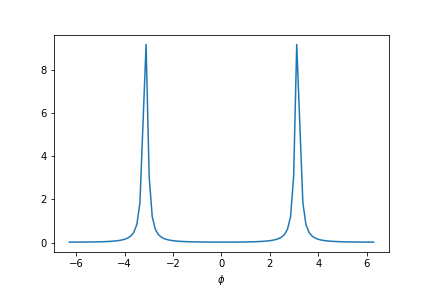
\includegraphics[width = 80mm]{./fig/ex7_15.png}
        \end{center}
    \end{figure}
\end{ex}

\begin{ex}
    \label{ex7.16}
    $m=\pm1$とする.
    \begin{align*}
        I \equiv \int Y_{l_1,m_1}^* Y_{1,m} Y_{l_2,m_2} d\Omega
         & \propto
        \int_{0}^\pi P_{l_1,m_1}(\cos \theta) \sin\theta P_{l_2,m_2}(\cos \theta) \ d\cos\theta
        \int_{0}^{2\pi} e^{i(-m_1+m+m_2)\phi}\ d\phi.
    \end{align*}
    $I$の$\phi$成分の積分に注目すると, $I \neq 0$であるためには,
    \begin{align*}
        \int_{0}^{2\pi} e^{i(-m_1+m+m_2)\phi}\ d\phi \neq 0
        \longleftrightarrow
        -m_1 + m + m_2 = 0
        \longleftrightarrow
        m_1 - m_2 = m = \pm1
    \end{align*}
    であることが必要.
    \par
    以下では$m=1$の場合だけ考えるが, $m=-1$の場合も同様である. 先の条件より,
    \begin{align*}
        m_1 = m_2 +1.
    \end{align*}
    Legendre陪多項式についての漸化式
    \begin{align*}
        \sin\theta P_{m,l}(\cos\theta)
        = \frac{1}{2l +1}\left[P_{l+1,m+1}(\cos \theta) - P_{l-1,m+1}(\cos\theta)\right]
    \end{align*}
    を用いて, $I$の$\theta$成分の積分は,
    \begin{align*}
           & \int_{0}^\pi P_{l_1,m_2 + 1}(\cos \theta) \sin\theta P_{l_2,m_2}(\cos \theta) \ d\cos\theta \\
        \  & =
        \frac{1}{2 l_2 + 1}\int_{0}^\pi P_{l_1,m_2+1}(\cos \theta)
        \left[P_{l_2+1,m_2+1}(\cos \theta) - P_{l_2-1,m_2+1}(\cos\theta)\right]
        \ d\cos\theta                                                                                    \\
    \end{align*}
    となる. よって, Legendre陪多項式の直交性より, $m=1$の時, $I$の$\theta$成分の積分が$0$にならないための必要十分条件は, $m_1 - m_2 = 1$かつ$l_1 = l_2 \pm 1$.
    \par
    以上より,
    \begin{align*}
        I \neq 0 \longleftrightarrow m_1 - m_2 = \pm 1 \mathrm{かつ} l_1 - l_2 = \pm1.
    \end{align*}
\end{ex}

\begin{ex}
    \label{ex7.17}
    $\omega = \delta = 0$のとき, Jaynes-CummingsのHamiltonian$H$は,
    \begin{align*}
        H = g \left( a^\dagger \sigma_- + a \sigma_+\right).
    \end{align*}
    よって,
    \begin{align*}
        H\ket{\chi_n}
         & =
        g \left( a^\dagger \sigma_- + a \sigma_+\right) \frac{\ket{n,1} + \ket{n+1, 0}}{\sqrt{2}}
        =
        g \frac{ \sqrt{n+1} \ket{n+1,0} + \sqrt{n+1}\ket{n, 1}}{\sqrt{2}}
        =
        g\sqrt{n+1}\ket{\chi_n}
        \\
        H\ket{\bar{\chi}_n}
         & =
        g \left( a^\dagger \sigma_- + a \sigma_+\right) \frac{\ket{n,1} - \ket{n+1, 0}}{\sqrt{2}}
        =
        g \frac{ \sqrt{n+1} \ket{n+1,0} - \sqrt{n+1}\ket{n, 1}}{\sqrt{2}}
        =
        -g\sqrt{n+1}\ket{\bar{\chi}_n}.
    \end{align*}
\end{ex}

\begin{ex}
    \label{ex7.18}
    時間発展演算子$U$は, $\Omega = \sqrt{g^2 + \delta^2}$を用いて,
    \begin{align*}
        U & =
        \exp \left[ - i H t \right]
        \\
          & =
        e^{ i \delta t } \ket{00}\bra{00}
        +
        \exp \left[
            i
            \begin{pmatrix}
                - \delta t & g t      \\
                gt         & \delta t
            \end{pmatrix}
            \right] \\
          & =
        e^{ i \delta t } \ket{00}\bra{00}+
        \exp \left[
            igt X - i\delta t Z
            \right] \\
          & =
        e^{ i \delta t } \ket{00}\bra{00}+
        I \cos \Omega t + i \frac{g}{\Omega} X \sin \Omega t - i \frac{\delta}{\Omega} Z \sin \Omega t
        \\
          & =
        e^{ i \delta t } \ket{00}\bra{00}+
        \left( \ket{01} \bra{01} + \ket{10}\bra{10}\right)\cos \Omega t
        + i \frac{g}{\Omega} \sin \Omega t  \left( \ket{01}\bra{10} + \ket{10}\ket{01}\right)
        - i \frac{\delta}{\Omega} \sin \Omega t \left( \ket{01} \bra{01} -\ket{10}\bra{10}\right)
        \\
          & =
        e^{ i \delta t } \ket{00}\bra{00}+
        \left( \cos \Omega t + i \frac{\delta}{\Omega} \sin\Omega t\right) \ket{01}\bra{01}
        +
        \left( \cos \Omega t + i \frac{\delta}{\Omega} \sin\Omega t\right) \ket{10}\bra{10}
        -
        i \frac{g}{\Omega} \sin\Omega t \left( \ket{01}\bra{10} + \ket{10}\bra{01}\right).
    \end{align*}
\end{ex}

\begin{ex}
    \label{ex7.19}
    \
    \begin{figure}[H]
        \begin{center}
            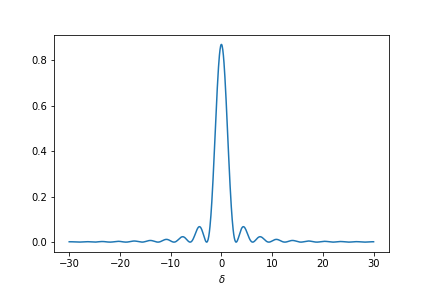
\includegraphics[width = 80mm]{./fig/ex7_19.png}
        \end{center}
    \end{figure}
\end{ex}

\begin{ex}
    \label{ex7.20}
    \
    \begin{figure}[H]
        \begin{center}
            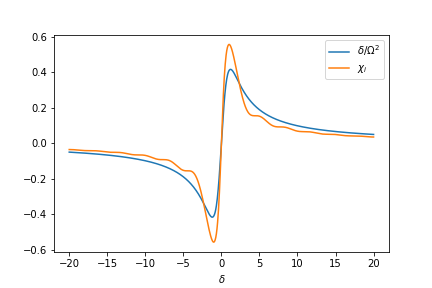
\includegraphics[width = 80mm]{./fig/ex7_20.png}
        \end{center}
    \end{figure}
\end{ex}

\begin{ex}
    \label{ex7.21}
    $\arg(\braket{110|U|110})$を求めるには, $U = \exp\left[ - i H t\right]$の$\ket{110}\bra{110}$成分だけ考えればよい. すると,
    \begin{align*}
        H_2^n
        =
        \begin{pmatrix}
            -\delta & g_a    & g_b    \\
            g_a     & \delta & 0      \\
            g_b     & 0      & \delta
        \end{pmatrix}^n
        =
        \begin{cases}
            \Omega'^{n} \ket{110}\bra{110} + ...\             & (n \mathrm{\ is\ even}) \\
            - \delta \Omega'^{n-1} \ket{110}\bra{110} + ...\  & (n \mathrm{\ is\ odd})
        \end{cases}
    \end{align*}
    なので,
    \begin{align*}
        \braket{110|U|110}
         & =
        \braket{110|\exp\left[ - i H t\right]|110}
        \\
         & =
        \braket{110|\exp\left[ - i H_2 t\right]|110}
        \\
         & =
        \braket{ 110|\sum_n \frac{1}{n!} (-i H_2 t)^n |110}
        \\
         & =
        \sum_{\mathrm{n\ is \ even}}
        \frac{(-1)^\frac{n}{2} t^n}{n!}
        \Omega'^{n}
        + i \delta
        \sum_{\mathrm{n\ is \ odd}}
        \frac{(-1)^\frac{n-1}{2} t^{n}}{n!}
        \Omega'^{n-1}
        \\
         & =
        \sum_{n}
        \frac{(-1)^n t^{2n}}{(2n)!}
        \Omega'^{2n}
        + i
        \frac{\delta}{\Omega'}
        \sum_{n}
        \frac{(-1)^n t^{2n+1}}{(2n+1)!}
        \Omega'^{2n+1}
        \\
         & =
        \cos\Omega' t + i \frac{\delta}{\Omega'} \sin\Omega't
    \end{align*}
    を得る. よって,
    \begin{align*}
        \phi_{ab} = \arg(\braket{110|U|110}) - \arg(\braket{000|U|000})
         & =\arg\left(\cos\Omega' t + i \frac{\delta}{\Omega'} \sin\Omega't \right) - \arg\left(e^{i \delta t}\right) \\
         & =
        \arg\left[\left(\cos\Omega' t + i \frac{\delta}{\Omega'} \sin\Omega't \right)e^{- i \delta t} \right].
    \end{align*}
    $\phi_a, \phi_b$については, $\Omega_i = \sqrt{g_i^2 + \delta^2}$として, 式(7.77)と全く同様の計算をして,
    \begin{align*}
        \phi_a
         & = \arg\left( \braket{100|U|100}\right) - \arg\left( \braket{000|U|000}\right)
        =  \arg\left[ \left(\cos\Omega_a t - i \frac{\delta}{\Omega_a} \sin\Omega_a t\right) e^{- i \delta t} \right]
        \\
        \phi_b
         & = \arg\left( \braket{010|U|010}\right) - \arg\left( \braket{010|U|010}\right)
        =  \arg\left[
        \left(\cos\Omega_b t - i \frac{\delta}{\Omega_b} \sin\Omega_b t \right)e^{- i \delta t} \right]
    \end{align*}
    \par
    以上より,
    \begin{align*}
        \chi_3 = \phi_{ab} - \phi_a - \phi_b
        =
        \arg\left[
            \frac{\cos\Omega' t + i \frac{\delta}{\Omega'} \sin\Omega't }
            {\left(\cos\Omega_a t - i \frac{\delta}{\Omega_a} \sin\Omega_a t\right)
                \left(\cos\Omega_b t - i \frac{\delta}{\Omega_b} \sin\Omega_b t \right)}
            e^{i \delta t}
            \right]
    \end{align*}
    $\chi_3$の$\delta$依存性を図示すると, 以下のようになる.
    \begin{figure}[H]
        \begin{center}
            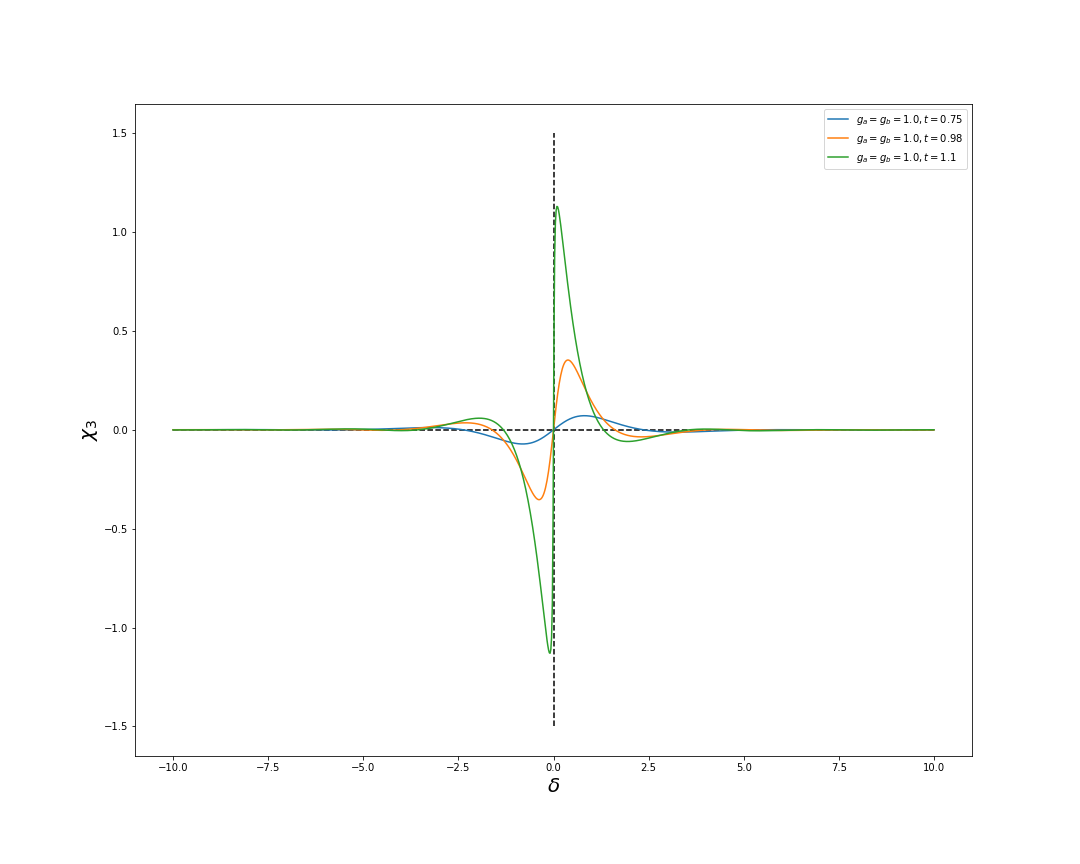
\includegraphics[width = 100mm]{./fig/ex7_21.png}
        \end{center}
    \end{figure}
\end{ex}

\begin{ex}
    \label{ex7.22}
    演習\ref{ex7.21}より, 光子が原子に吸収される確率は,
    \begin{align*}
        1 - \left| \braket{110|U|110}\right|^2
        =  1 - \left(\cos\Omega' t\right)^2 - \left(\frac{\delta}{\Omega'} \sin\Omega't \right)^2
    \end{align*}
    図示すると, 以下のようになる.
    \begin{figure}[H]
        \begin{center}
            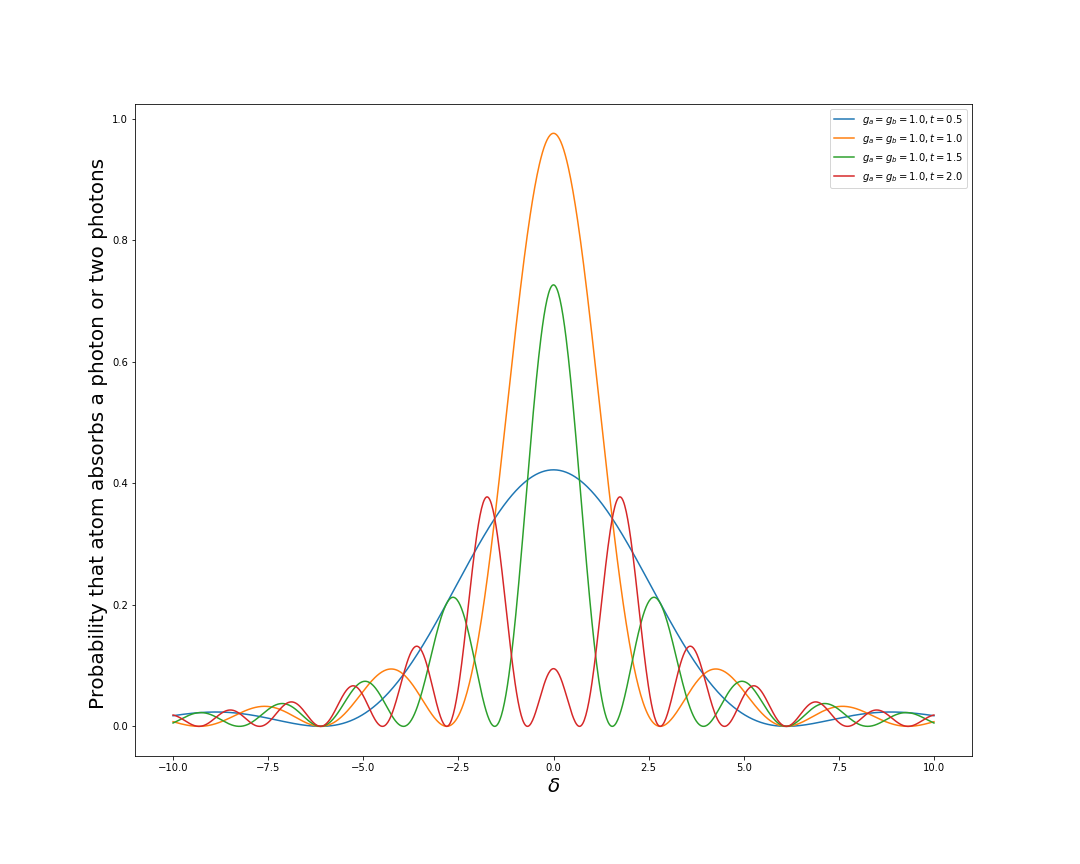
\includegraphics[width = 100mm]{./fig/ex7_22.png}
        \end{center}
    \end{figure}
\end{ex}

\begin{ex}
    \label{ex7.23}
\end{ex}
\begin{ex}
    \label{ex7.24}
    \begin{align*}
        \mu_N B \sim 5 \times 10^{-26} \ J < k_B T \sim 5 \times 10^{-21} J
    \end{align*}
\end{ex}

\begin{ex}
    \label{ex7.25}
    \begin{align*}
        \left[ j_i , j_k \right]
         & =
        \left[
            \frac{ \sigma_i \otimes I + I \otimes \sigma_i}{2},
            \frac{\sigma_k \otimes I + I \otimes \sigma_k}{2}
            \right]                                                        \\
         & =
        \frac{\left[\sigma_i \otimes I,\sigma_k \otimes I \right]
            +
            \left[I\otimes \sigma_i , I\otimes \sigma_k \right]
        }{4}                                                               \\
         & =
        i \epsilon_{ikl} \frac{\sigma_l \otimes I + I \otimes \sigma_l}{2} \\
         & =
        i \epsilon_{ikl}  j_l.
    \end{align*}
\end{ex}

\begin{ex}
    \label{ex7.26}
    \begin{align*}
        J^2 =
        \begin{pmatrix}
            0 & 0 & 0 & 0 \\
            0 & 2 & 0 & 0 \\
            0 & 0 & 2 & 0 \\
            0 & 0 & 0 & 2 \\
        \end{pmatrix},\
        j_z = \begin{pmatrix}
            0 & 0  & 0 & 0 \\
            0 & -1 & 0 & 0 \\
            0 & 0  & 0 & 0 \\
            0 & 0  & 0 & 1 \\
        \end{pmatrix}
    \end{align*}
\end{ex}

\begin{ex}
    \label{ex7.27}
\end{ex}

\begin{ex}
    \label{ex7.28}
    (1)\
    \begin{align*}
        \left[ i_k, i_l\right] = i \epsilon_{klm}i_m.
    \end{align*}
    \par
    (2)
    \begin{align*}
        \ket{2,2}, \ket{2,1}, \ket{2,0}, \ket{2,-1}, \ket{2,-2},
        \ket{1,1}, \ket{1,0}, \ket{1,-1}.
    \end{align*}
\end{ex}

\begin{ex}
    \label{ex7.29}
    \begin{align*}
        \int_0^\infty
        \frac
        {\sin^2\frac{\omega - \omega_0}{2}t}
        {\left(\omega - \omega_0\right)^2}
        \omega
        \ dw
        \sim
        \int_{-\infty}^\infty
        \frac
        {\sin^2\frac{\omega - \omega_0}{2}t}
        {\left(\omega - \omega_0\right)^2}
        \omega_0
        \ dw
        =
        \int_{-\infty}^\infty
        \frac
        {t^2\sin^2\frac{\omega - \omega_0}{2}t}
        { 4\left(\frac{\omega - \omega_0}{2}t\right)^2}
        \omega_0
        \ dw
        =
        \int_{-\infty}^\infty
        \frac
        {t\sin^2 x}
        { 2x^2}
        \omega_0
        \ dx
        =
        \frac{\pi t \omega_0}{2}.
    \end{align*}
    ここで, $\sim$では, 被積分関数の寄与が$\omega \sim \omega_0$で非常に大きいことを用いた. この結果を用いて,
    \begin{align*}
        \gamma_\mathrm{rad}
         & =
        \frac{d}{dt} \frac{1}{\left( 2 \pi c\right)^2}\frac{8 \pi}{3}
        \int_0^\infty \omega^2 p_\mathrm{decay} \ d\omega
        \\
         & =
        \frac{d}{dt}
        \frac{1}{\left( 2 \pi c\right)^2}\frac{8 \pi}{3}
        \int_0^\infty
        \frac{\omega_0^2 \left| \braket{0|\bm{\mu}|1} \right|^2}{2 \hbar \omega \epsilon_0 c^3}
        \frac{4\sin^2\frac{\omega - \omega_0}{2}t}{\left(\omega - \omega_0\right)^2}
        \omega^2
        \ d\omega                                                                                      \\
         & = \frac{\omega_0^3  \left| \braket{0|\bm{\mu}|1} \right|^2 }{3 \pi \hbar \epsilon_0 c^5}\ .
    \end{align*}
\end{ex}

\begin{ex}
    \label{ex7.30}
    \begin{align*}
        \frac{\gamma_\mathrm{rad}^\mathrm{ed} }{\gamma_\mathrm{rad}}
        =
        \frac{\left| \braket{0|\bm{\mu}_\mathrm{ed}|1} \right|^2}{\left| \braket{0|\bm{\mu}|1} \right|^2}
        \sim
        \frac{e^2 a_0^2 \omega_0^\mathrm{ed}}{\mu_B^2 \omega_0}
        \sim
        \frac{10^{-58} 10^{15}}{10^{-46} 10^{10}} = 10^{-7}.
    \end{align*}
\end{ex}

\begin{ex}
    \label{ex7.31}
    \begin{align*}
        H = e^{i \frac{\pi}{2}} R_x \left( \pi\right) R_y \left( \frac{\pi}{2}\right).
    \end{align*}
\end{ex}

\begin{ex}
    \label{ex7.32}

\end{ex}

\begin{ex}
    \label{ex7.33}
    \begin{align*}
        i \frac{\partial}{\partial t} \ket{\phi(t)}
         & =
        i \frac{\partial}{\partial t} e^{\frac{i \omega Z t}{2}} \ket{ \chi(t)} \\
         & =
        - \frac{\omega Z}{2} e^{\frac{i \omega Z t}{2}}\ket{\chi(t)}
        +
        i e^{\frac{i \omega Z}{2}} \frac{\partial}{\partial t}\ket{ \chi(t)}    \\
         & =
        - \frac{\omega Z}{2} e^{\frac{i \omega Z}{2}} \ket{\chi(t)}
        +
        e^{\frac{i \omega Z}{2}} H \ket{\chi(t)}                                \\
         & =
        \left[e^{\frac{i \omega Z}{2}} H e^{ -\frac{i \omega Z}{2}} - \frac{\omega Z}{2} e^{\frac{i \omega Z}{2}} \right] \ket{\phi(t)}.
    \end{align*}
\end{ex}

\begin{ex}
    \label{ex7.34}
\end{ex}
\begin{ex}
    \label{ex7.35}
    $H_{1,2}^D$の球面平均は, その定数項の寄与を除いて,
    \begin{align*}
         & \ \ \ \ \
        \int_0^\pi d \theta \int_0^{2 \pi} d \phi
        \ \sin\theta
        \left[
            \bm{\sigma}_1 \cdot \bm{\sigma}_2
            -
            3
            \left( \bm{\sigma}_1 \cdot \bm{n}\right)
            \left(  \bm{\sigma}_2 \cdot \bm{n}\right)
            \right]                                        \\
         & =
        \int_0^\pi d \theta \int_0^{2 \pi} d \phi \
        \sigma_{1x}\sigma_{2x}
        \left( \sin\theta - 3 \sin^3\theta \cos^2\phi\right)
        +
        \sigma_{1y}\sigma_{2y}
        \left( \sin\theta - 3 \sin^3\theta \sin^2\phi\right)
        +
        \sigma_{1z}\sigma_{2z}
        \left( \sin\theta - 3 \cos^2\theta \sin\theta\right)
        \\
         & \ \ \ \ \ \ \ \ \ \ \ \ \ \ \ \ \ \ \ \ \ \ \ \
        +\sin^3\theta \sin\phi \cos\phi
        \left( \sigma_{1x} \sigma_{2y} + \sigma_{1y}\sigma_{2x}\right)
        +
        \sin^3\theta \cos\theta \cos\phi
        \left( \sigma_{1x} \sigma_{2z} + \sigma_{1z}\sigma_{2x}\right)
        \\
         & \ \ \ \ \ \ \ \ \ \ \ \ \ \ \ \ \ \ \ \ \ \ \ \
        +
        \sin^2\theta \cos\theta \sin\phi
        \left( \sigma_{1y} \sigma_{2z} + \sigma_{1z}\sigma_{2y}\right)
        \\&=0
    \end{align*}
\end{ex}

\begin{ex}
    \label{ex7.36}
    \underline{$n=1$}\par
    考えるべきは, 2準位系で, そのエネルギーを$\frac{\hbar \omega}{2}, -\frac{\hbar \omega}{2}$とする.
    すると, 基底としてエネルギー固有状態を考えた行列表示で, $\beta \ll 1$とすると,
    \begin{align*}
        e^{- \beta H} \sim 1 - \beta H = 1 - \frac{\beta \hbar \omega}{2}
        \begin{pmatrix}
            1 & 0  \\
            0 & -1
        \end{pmatrix}
    \end{align*}
    \underline{$n=2$}\par
    2つの2準位系;
    \begin{align*}
        A: & \ - \frac{\omega_A}{4} ,\ \frac{\omega_A}{4} \\
        B: & \ - \frac{\omega_B}{4} ,\ \frac{\omega_B}{4} \\
    \end{align*}
    を考えると,
    \begin{align*}
        e^{- \beta H} \sim 1 - \beta H
        = 1 - \beta \hbar
        \begin{pmatrix}
            \omega_A + \omega_B & 0                   & 0                   & 0                    \\
            0                   & \omega_B - \omega_A & 0                   & 0                    \\
            0                   & 0                   & \omega_A - \omega_B & 0                    \\
            0                   & 0                   & 0                   & - \omega_A -\omega_B
        \end{pmatrix}
        =
        1-
        \frac{\beta \hbar \omega_A}{4}
        \begin{pmatrix}
            5 & 0 & 0  & 0  \\
            0 & 3 & 0  & 0  \\
            0 & 0 & -3 & 0  \\
            0 & 0 & 0  & -5
        \end{pmatrix}
    \end{align*}
\end{ex}

\begin{ex}
    \label{ex7.37}
    まず,
    \begin{align*}
        H = J Z_1 \otimes Z_2
    \end{align*}
    のとき,
    \begin{align*}
        e^{-iHt} = I \otimes I \cos Jt - i Z_1 \otimes Z_2 \sin Jt
        =
        \begin{pmatrix}
            e^{-i Jt} & 0       & 0       & 0        \\
            0         & e^{iJt} & 0       & 0        \\
            0         & 0       & e^{iJt} & 0        \\
            0         & 0       & 0       & e^{-iJt}
        \end{pmatrix}.
    \end{align*}
    次に,
    \begin{align*}
        \rho & =
        \exp \left[ i \pi \frac{Y_1 \otimes I}{4} \right]
        \frac{1}{4}
        \left[
            1 - \beta \hbar \omega_0 \left( Z_1 \otimes I + I \otimes Z_2\right) \right]
        \exp \left[ -i \pi \frac{Y_1 \otimes I}{4} \right]
        \\
             & =
        \frac{1}{4}
        \left[
            1 - \beta \hbar \omega_0 \left( - X_1 \otimes I + I \otimes Z_2\right) \right].
    \end{align*}
    よって,
    \begin{align*}
        e^{-iHt} \rho e^{iHt}
        =
        \frac{1}{4}
        \begin{pmatrix}
            1 - \beta \hbar \omega_0      & 0                              & \beta \hbar \omega_0 e^{-2iJt} & 0                             \\
            0                             & 1+\beta \hbar \omega_0         & 0                              & \beta \hbar \omega_0 e^{2iJt} \\
            \beta \hbar \omega_0 e^{2iJt} & 0                              & 1 - \beta \hbar \omega_0       & 0                             \\
            0                             & \beta \hbar \omega_0 e^{-2iJt} & 0                              & 1 + \beta\hbar \omega_0
        \end{pmatrix}.
    \end{align*}
    したがって,
    \begin{align*}
        V(t)
         & = V_0 \ \tr \left[  e^{-iHt} \rho e^{iHt} \left( i X_1 + Y_1\right) \otimes I \right]
        \\
         & =   \frac{i V_0 \beta \hbar \omega_0}{2} \ \tr
        \left[
            \begin{pmatrix}
                e^{2i Jt} & 0         & 0 & 0 \\
                0         & e^{-2iJt} & 0 & 0 \\
                0         & 0         & 0 & 0 \\
                0         & 0         & 0 & 0
            \end{pmatrix}
            \right]
        \\
         & = i V_0 \beta \hbar \omega_0 \cos Jt.
    \end{align*}

\end{ex}

\begin{ex}
    \label{ex7.38}
    演習\ref{ex4.7}と同様に,
    \begin{align*}
        X R_z(\theta) X = R_z(-\theta)
    \end{align*}
    であることから,
    \begin{align*}
        R_x(\pi) e^{- i a Z_1 t} R_x(\pi)
        =
        (-iX)  R_z(2at) (-iX)
        =
        - R_z(-2at)
        =
        - e^{i a Z_1 t}.
    \end{align*}
\end{ex}

\begin{ex}
    \label{ex7.39}
    $R_x = R_x\left( \frac{\pi}{2}\right), \ R_y = R_y\left( \frac{\pi}{2}\right)$とする.
    演習\ref{ex7.38}と同様に,
    \begin{align*}
        R_x^2 e^{- i c_y \sigma_y} R_x^2 =  -e^{i c_y  \sigma_y} \\
        R_x^2 e^{- i c_z \sigma_z} R_x^2 =  -e^{i c_z  \sigma_z} \\
        R_y^2 e^{- i c_x \sigma_x} R_y^2 = -e^{i c_x \sigma_x}
    \end{align*}
    である. このことを用いて,
    \begin{align*}
        H = \sum_k c_k \sigma_k
    \end{align*}
    に対して,
    \begin{align*}
        e^{-iHt} R_x^2 e^{-iHt} R_x^2             & =  -e^{-2ic_x \sigma_x t}                                   \\
        R_y^2 e^{-iHt} R_x^2 e^{-iHt} R_x^2 R_y^2 & = - R_y^2 e^{-2ic_x \sigma_x t} R_y^2 =e^{2ic_x \sigma_x t}
    \end{align*}
    となるから,
    \begin{align*}
        R_y^2 e^{-iHt} R_x^2 e^{-iHt} R_x^2 R_y^2 e^{-iHt} R_x^2 e^{-iHt} R_x^2
        = -e^{2ic_x \sigma_x t} e^{-2ic_x \sigma_x t}
        =-1
    \end{align*}
    というようなパルス列を与えると, 系の時間発展を再収束させられる.
\end{ex}

\begin{ex}
    \label{ex7.41}
\end{ex}

\begin{ex}
    \label{ex7.41}
    \begin{align*}
        H = a Z_1 + b Z_2 + c Z_1 Z_2
    \end{align*}
    のとき,
    \begin{align*}
        e^{-i H t}R_{x1}^2 e^{-i H t}R_{x1}^2 = -e^{-2ibZ_2 t}                    \\
        e^{-i H t}R_{x2}^2 e^{-i H t}R_{x2}^2 = -e^{-2iaZ_1 t}                    \\
        e^{-i H t}R_{x1}^2R_{x2}^2 e^{-i H t}R_{x1}^2R_{x2}^2 = e^{-2icZ_1 Z_2 t} \\
    \end{align*}
    であることと演習\ref{ex7.47}より,
    \begin{align*}
        e^{-i \frac{\pi}{4}} U_{CNOT}
         & = e^{i \frac{\pi}{4}Z_2}e^{-i\frac{\pi}{4}Z_1}R_{x2} e^{-i \frac{\pi}{2} Z_1 Z_2}  R_{y2} \\
         & =
        e^{i H \frac{\pi}{8b}}R_{x1}^2 e^{i H \frac{\pi}{8b}}R_{x1}^2
        e^{ - i H \frac{\pi}{8a}}R_{x2}^2 e^{ - i H \frac{\pi}{8a}}R_{x2}^2
        R_{x2} e^{-i H \frac{\pi}{8c}}R_{x1}^2R_{x2}^2 e^{-i H \frac{\pi}{8c}}R_{x1}^2R_{x2}^2 R_{y2}.
    \end{align*}
\end{ex}

\begin{ex}
    \label{ex7.42}
    $P$は,
    \begin{align*}
        \Qcircuit @C=1em @R=1em {
        \lstick{} & \targ     & \ctrl{1} & \qw \\
        \lstick{} & \ctrl{-1} & \targ    & \qw
        }
    \end{align*}
    $P^\dagger$は,
    \begin{align*}
        \Qcircuit @C=1em @R=1em {
        \lstick{} & \ctrl{1} & \targ     & \qw \\
        \lstick{} & \targ    & \ctrl{-1} & \qw
        }
    \end{align*}
\end{ex}

\begin{ex}
    \label{ex7.43}
    \begin{align*}
        \Qcircuit @C=1em @R=1em {
        \lstick{} & \qw       & \ctrl{2} & \targ     & \qw \\
        \lstick{} & \targ     & \qw      & \ctrl{-1} & \qw \\
        \lstick{} & \ctrl{-1} & \targ    & \qw       & \qw
        }
    \end{align*}
\end{ex}

\begin{ex}
    \label{ex7.44}
    簡単のため$n$を偶数とする.
    Zeemann周波数$\omega$のspinが$n$個ある系の密度行列$\rho$は,
    \begin{align*}
        Z = e^{\beta \hbar \omega} + e^{- \beta \hbar \omega}
    \end{align*}
    として,
    \begin{align*}
        \rho
        =
        \frac{1}{Z^n}
        \begin{pmatrix}
            e^{\beta \hbar \omega} & 0                        \\
            0                      & e^{- \beta \hbar \omega}
        \end{pmatrix}^{\otimes n}.
    \end{align*}
    特に$\beta \hbar \omega \ll  1$では,
    \begin{align*}
        \rho \sim
        \frac{1}{2^n}
        \left[
            I + \beta \hbar \omega
            \begin{pmatrix}
                1 & 0  \\
                0 & -1
            \end{pmatrix}
            \right]^{\otimes n}.
    \end{align*}
    以下$O(\beta \hbar \omega)$まで考えるとする. 少し頑張って考えると, $\rho$の対角成分の$0$の個数は$2^{\frac{n}{2}+1} - 2$個, $\rho$の(0,0)成分は$\frac{n\beta \hbar \omega}{2^n}$になる. したがって,
    式(7.163)から式(7.165)と全く同様の手続きを行えば,
    \begin{align*}
        \exists \tilde{P} \ \ \ \left( \tilde{P} \rho \tilde{P}^\dagger - \frac{I^{\otimes n}}{2^n} \mathrm{の上} (2^{\frac{n}{2}+1} - 2) \times (2^{\frac{n}{2}+1} - 2)\mathrm{ブロック} \right)
        = \frac{n \beta \hbar \omega }{2^n}\underbrace{\ket{00...00}}_{2^{\frac{n}{2}+1}-2 \ qubit}\bra{00...00}.
    \end{align*}
    $n$が偶数の時, $\rho$の対角成分の値に注目すると$0$が一番多いので, 上に示したものが, 論理ラベルで作れる実効的純粋状態のうち最大のqubit数を持つものである.
\end{ex}

\begin{ex}
    \label{ex7.45}
    密度行列$\rho$は$r_{ij} \in \mathbb{R} \ (i,j = 1,2,3)$を用いて,
    \begin{align*}
        \rho = \frac{1}{4} \left[ I \otimes I + \sum_{i, j} r_{ij} \sigma_i \otimes \sigma_j \right]
    \end{align*}
    かける. この$\rho$の各係数$r_{ij}$を決めるには,
    \begin{align*}
        \langle \sigma_i \otimes \sigma_j \rangle = \tr \left[ \rho \sigma_i \otimes \sigma_j \right] =r_{ij}
    \end{align*}
    より, $\sigma_i \otimes \sigma_j$を測定すれば良い. つまり9回の測定をすれば良い.
\end{ex}

\begin{ex}
    \label{ex7.46}
    27回測定すれば十分.
\end{ex}

\begin{ex}
    \label{ex7.47}
    \begin{align*}
        R_{x2} e^{-i \frac{\pi}{4} Z_1 Z_2} R_{y2}
         & =
        \frac{1}{\sqrt{2}}
        \begin{pmatrix}
            1 & -1 & 0 & 0  \\
            1 & 1  & 0 & 0  \\
            0 & 0  & 1 & -1 \\
            0 & 0  & 1 & 1
        \end{pmatrix}
        e^{-i\frac{\pi}{4}}
        \begin{pmatrix}
            1 & 0 & 0 & 0 \\
            0 & i & 0 & 0 \\
            0 & 0 & i & 0 \\
            0 & 0 & 0 & 1
        \end{pmatrix}
        \frac{1}{\sqrt{2}}
        \begin{pmatrix}
            1  & -i & 0  & 0  \\
            -i & 1  & 0  & 0  \\
            0  & 0  & 1  & -i \\
            0  & 0  & -i & 1
        \end{pmatrix}
        \\
         & =
        e^{-i \frac{\pi}{4}}
        \begin{pmatrix}
            1 & 0 & 0 & 0  \\
            0 & i & 0 & 0  \\
            0 & 0 & 0 & -i \\
            0 & 0 & 1 & 0
        \end{pmatrix}
    \end{align*}
    であり,
    \begin{align*}
        e^{i \frac{\pi}{4}Z_2}e^{-i\frac{\pi}{4}Z_1}R_{x2} e^{-i \frac{\pi}{4} Z_1 Z_2}  R_{y2}
         & =
        \begin{pmatrix}
            e^{i\frac{\pi}{4}} & 0                   & 0                  & 0                    \\
            0                  & e^{-i\frac{\pi}{4}} & 0                  & 0                    \\
            0                  & 0                   & e^{i\frac{\pi}{4}} & 0                    \\
            0                  & 0                   & 0                  & e^{ーi\frac{\pi}{4}}
        \end{pmatrix}
        \begin{pmatrix}
            e^{-i\frac{\pi}{4}} & 0                   & 0                  & 0                  \\
            0                   & e^{-i\frac{\pi}{4}} & 0                  & 0                  \\
            0                   & 0                   & e^{i\frac{\pi}{4}} & 0                  \\
            0                   & 0                   & 0                  & e^{i\frac{\pi}{4}}
        \end{pmatrix}
        e^{-i \frac{\pi}{4}}
        \begin{pmatrix}
            1 & 0 & 0 & 0  \\
            0 & i & 0 & 0  \\
            0 & 0 & 0 & -i \\
            0 & 0 & 1 & 0
        \end{pmatrix}
        \\
         & =
        e^{-i\frac{\pi}{4}}
        \begin{pmatrix}
            1 & 0 & 0 & 0 \\
            0 & 1 & 0 & 0 \\
            0 & 0 & 0 & 1 \\
            0 & 0 & 1 & 0
        \end{pmatrix}
        =
        e^{-i\frac{\pi}{4}}U_{CNOT}.
    \end{align*}
\end{ex}

\begin{ex}
    \label{ex7.48}
    \begin{align*}
        R_{x2} e^{-i \frac{\pi}{4} Z_1 Z_2} R_{y2}R_{y1}
         & =
        e^{-i\frac{\pi}{4}}
        \begin{pmatrix}
            1 & 0 & 0 & 0  \\
            0 & i & 0 & 0  \\
            0 & 0 & 0 & -i \\
            0 & 0 & 1 & 0
        \end{pmatrix}
        \frac{1}{\sqrt{2}}
        \begin{pmatrix}
            1  & 0  & -1 & 0  \\
            0  & 1  & 0  & -1 \\
            -1 & 0  & 1  & 0  \\
            0  & -1 & 0  & 1
        \end{pmatrix}
        \\
         & =
        \frac{e^{-i \frac{\pi}{4}}}{\sqrt{2}}
        \begin{pmatrix}
            1 & 0  & -1 & 0  \\
            0 & i  & 0  & -i \\
            0 & -i & 0  & -i \\
            1 & 0  & 1  & 0
        \end{pmatrix} \\
    \end{align*}
    より, $ R_{x2} e^{-i \frac{\pi}{4} Z_1 Z_2} R_{y2}R_{y1}$は,
    \begin{align*}
        \ket{00} \to \frac{\ket{00} + \ket{11}}{\sqrt{2}} \\
        \ket{01} \to \frac{\ket{01} - \ket{10}}{\sqrt{2}} \\
        \ket{10} \to \frac{\ket{00} - \ket{11}}{\sqrt{2}} \\
        \ket{00} \to \frac{\ket{01} + \ket{10}}{\sqrt{2}} \\
    \end{align*}
    というようにBell状態を作る.
\end{ex}

\begin{ex}
    \label{ex7.49}
    演習\ref{ex7.47}でCNOTがいかに作れるかを示したことを思い出して,
    \begin{align*}
        SWAP
         & = C(X_2) C(X_1) C(X_2)  \\
         & = e^{-i \frac{3\pi}{4}}
        e^{i \frac{\pi}{4}Z_2}e^{-i\frac{\pi}{4}Z_1}R_{x2} e^{-i \frac{\pi}{4} Z_1 Z_2}  R_{y2}
        e^{i \frac{\pi}{4}Z_1}e^{-i\frac{\pi}{4}Z_2}R_{x1} e^{-i \frac{\pi}{4} Z_1 Z_2}  R_{y1}
        e^{i \frac{\pi}{4}Z_2}e^{-i\frac{\pi}{4}Z_1}R_{x2} e^{-i \frac{\pi}{4} Z_1 Z_2}  R_{y2}.
    \end{align*}
\end{ex}

\begin{ex}
    \label{ex7.50}
\end{ex}

\begin{ex}
    \label{ex7.51}
    $x_0 = 3$の時だけ示す.
    $R_{?i}$と$R_{?j}$は$i \neq j$のとき可換で, $R_x^3 = \bar{R}_x, R_y^3 = \bar{R}_y$であることを用いて,
    \begin{align*}
        G
        = H^{\otimes2} P H^{\otimes2} O
         & =
        R_{x1}^2 \cancel{\bar{R}_{y1}}R_{x2}^2 \bcancel{\bar{R}_{y2}}
        \cancel{R_{y1}}R_{x1}\bar{R}_{y1} \bcancel{R_{y2}}R_{x2}\bar{R}_{y2}\tau
        R_{x1}^2 \cancel{\bar{R}_{y1}}R_{x2}^2 \bcancel{\bar{R}_{y2}}
        \cancel{R_{y1}}\bar{R}_{x1}\bar{R}_{y1}\bcancel{R_{y2}}\bar{R}_{x2}\bar{R}_{y2} \tau
        \\
         & =
        R_{x1}^2 R_{x2}^2
        R_{x1}\bar{R}_{y1}R_{x2}\bar{R}_{y2}\tau
        R_{x1}^2 R_{x2}^2
        \bar{R}_{x1}\bar{R}_{y1}\bar{R}_{x2}\bar{R}_{y2} \tau
        \\
         & =
        R_{x1}^3 R_{x2}^3
        \bar{R}_{y1}\bar{R}_{y2}\tau
        R_{x1}
        \bar{R}_{y1}\bar{R}_{y2} \tau
        \\
         & =
        \bar{R}_{x1} \bar{R}_{x2}
        \bar{R}_{y1}R_{x2}\bar{R}_{y2}\tau
        R_{x1} R_{x2}
        \bar{R}_{y1}\bar{R}_{y2} \tau.
    \end{align*}
\end{ex}




\chapter{量子雑音と量子情報}

\begin{ex}
    \label{ex8.1}
    \begin{align*}
        \qo(\rho)
        =
        U \ket{\psi} \bra{\psi} U^\dagger
        =
        U \rho U^\dagger
    \end{align*}
\end{ex}

\begin{ex}
    \label{ex8.2}
    密度行列は, スペクトル分解可能;
    \begin{align*}
        \rho = \sum_i p_i \ket{i} \bra{i}.
    \end{align*}
    測定オペレータの集合$\{ M_m\}$に対し, $\rho$の測定結果が$m$である確率は,
    \begin{align*}
        p(m) =
        \sum_i p(m|i) p_i
        =
        \sum_i \braket{i | M_m^\dagger M_m | i} p_i
        =
        \tr \left[ \sum_i \braket{i | M_m^\dagger M_m | i} p_i \right]
        =
        \tr \left[ M_m^\dagger M_m \rho\right]
        =
        \tr \left[M_m \rho  M_m^\dagger \right].
    \end{align*}
    測定後の系の状態$\rho_m$は,
    \begin{align*}
        \left\{ \ket{i^m} =
        \frac{M_m \ket{i}}{\sqrt{\braket{i|M_m^\dagger M_m | i}}},
        p(i|m)
        \right\}
    \end{align*}
    というアンサンブルで,
    \begin{align*}
        \rho_m
        =
        \sum_i p(i|m) \ket{i^m} \bra{i^m}
        =
        \sum_i
        \frac{p(m|i) p_i}{p(m)}
        \frac{M_m \ket{i} \bra{i} M_m^\dagger}
        {\braket{i|M_m^\dagger M_m | i}}
        =
        \sum_i p(i|m) \ket{i^m} \bra{i^m}
        =
        \sum_i
        \frac{p_i M_m \ket{i} \bra{i} M_m^\dagger}{p(m)}
        =
        \frac{M_m \rho M_M^\dagger}
        {\tr\left[ M_m \rho M_m^\dagger\right]}
    \end{align*}
\end{ex}

\begin{ex}
    \label{ex8.3}
    ABの初期状態$\rho_A \otimes \rho_B = \rho =
        \sum_{a,b} p_{ab} \ket{a}\bra{a} \otimes \ket{b}\bra{b}$,
    CDの初期状態$\ket{0_C}\bra{0_C} \otimes \ket{0_D}\bra{0_D}$
    として,
    \begin{align*}
        \qo\left(\rho\right)
         & =
        \tr_{A \otimes D}
        \left[
            U \rho \otimes \ket{0_C}\bra{0_C} \otimes \ket{0_D}\bra{0_D} U^\dagger
            \right]
        \\
         & =
        \sum_{a,a', b, d'}
        p_{ab}
        \bra{a'} \otimes \bra{d'}
        \left(
        U \ket{a} \bra{a} \otimes \ket{b}\bra{b} \otimes \ket{0}\bra{0} \otimes \ket{0}\bra{0} U^\dagger
        \right)
        \ket{a'} \otimes \ket{d'}
        \\
         & =
        \sum_{a,a', b, d'}
        p_{ab}
        \bra{a'} \otimes \bra{d'}
        U
        \ket{0_C} \otimes \ket{0_D}
        \ket{a}\bra{a} \otimes \ket{b}\bra{b}
        \bra{0_C} \otimes \bra{0_D}
        U^\dagger
        \ket{a'} \otimes \ket{d'}
        \\
         & =
        \sum_{a',d'}
        \bra{a'} \otimes \bra{d'}
        U
        \ket{0_C} \otimes \ket{0_D}
        \rho
        \bra{0_C} \otimes \bra{0_D}
        U^\dagger
        \ket{a'} \otimes \ket{d'} =
        \sum_{a,d}
        E_{ad}
        \rho
        E_{ad}^\dagger.
    \end{align*}
    ただし,
    \begin{align*}
        E_{ad} = \bra{a'} \otimes \bra{d'}
        U
        \ket{0_C} \otimes \ket{0_D}
    \end{align*}
    で, ADでの完全性条件より,
    \begin{align*}
        \sum_{a,d}
        E_{ad}
        E_{ad}^\dagger
         & =
        \sum_{a,d}
        \bra{a'} \otimes \bra{d'}
        U
        \ket{0_C} \otimes \ket{0_D}
        \bra{0_C} \otimes \bra{0_D}
        U^\dagger
        \ket{a'} \otimes \ket{d'}
        \\
         & =
        \sum_{a,d}
        \bra{0_C} \otimes \bra{0_D}
        U^\dagger
        \ket{a'} \otimes \ket{d'}
        \bra{a'} \otimes \bra{d'}
        U
        \ket{0_C} \otimes \ket{0_D}
        \\
         & =
        \bra{0_C} \otimes \bra{0_D}
        U^\dagger
        U
        \ket{0_C} \otimes \ket{0_D} = I_{AB}.
    \end{align*}
\end{ex}

\begin{ex}
    \label{ex8.4}
    環境の初期状態$\ket{0}$として,
    \begin{align*}
        E_k
        = \left(I \otimes \bra{k}\right)   U  \left(I \otimes \ket{0}\right)
        = 
        \left(I \otimes \bra{k}\right)  
        \left( P_0 \otimes I + P_1 \otimes X  \right)
        \left(I \otimes \ket{0}\right)
        = P_0 \braket{k|0} + P_1 \braket{k|1}.
    \end{align*}
    なので, オペレータ和表現は, 
    \begin{align*}
        \qo (\rho)
        = \sum_{k = 0, 1} E_k \rho E_k^\dagger
        = P_0 \rho P_0 + P_1 \rho P_1.
    \end{align*}
\end{ex}

\begin{ex}
    \label{ex8.5}
    環境の初期状態$\ket{0}$として,
    \begin{align*}
        E_k
        = \braket{k | U | 0}
        = \frac{X}{\sqrt{2}} \braket{k|0} + \frac{Y}{\sqrt{2}} \braket{k|1}.
    \end{align*}
    なので, 量子演算は,
    \begin{align*}
        \qo (\rho)
        = \sum_{k = 0, 1} E_k \rho E_k^\dagger
        = \frac{X \rho X + Y \rho Y}{2}.
    \end{align*}
\end{ex}

\begin{ex}
    \label{ex8.6}
    \par
    CP写像$\qo \colon \linearopset{\mathbb{C}^m} \to \linearopset{\mathbb{C}^n}$の演算要素$\left\{E_k \colon \mathbb{C}^m \to \mathbb{C}^n \right\}_{k=1}^{l_E \le nm}$, CP写像$\qof \colon \linearopset{\mathbb{C}^n} \to \linearopset{\mathbb{C}^m}$演算要素$\left\{F_k \colon \mathbb{C}^n \to \mathbb{C}^m \right\}_{k=1}^{l_F \le nm}$とする. このとき, 合成写像$\qo \circ \qof \colon \linearopset{\mathbb{C}^n} \to \linearopset{\mathbb{C}^n}$は, $A \in \linearopset{\mathbb{C}^n}$に対して,
    \begin{align*}
        \qo \circ \qof \left( A\right)
        =
        \sum_{i = 1}^{l_E}\sum_{j=1}^{l_F}
        E_i F_j A F_j^\dagger E_i^\dagger
    \end{align*}
    でかける. 演習\ref{ex8.10}より, $\qo \circ \qof \colon \linearopset{\mathbb{C}^n} \to \linearopset{\mathbb{C}^n}$の演算要素$\left\{G_i \colon \mathbb{C}^n \to \mathbb{C}^n \right\}_{i=1}^{l_G \le nm}$を作ることができる. したがって, $\qo \circ \qof \colon \linearopset{\mathbb{C}^n} \to \linearopset{\mathbb{C}^n}$もCP写像.
\end{ex}

\begin{ex}
    \label{ex8.7}
    \begin{align*}
        \qo_m \left( \rho \right)
        =
        \tr_E \left( M_m U \rho \otimes \sigma U^\dagger M_m^\dagger \right)
    \end{align*}
    として, Qの終状態は,
    \begin{align*}
        \frac{\qo_m \left( \rho \right)}{\tr \left[ \qo_m(\rho)\right]}
    \end{align*}
    で,
    \begin{align*}
        \sigma = \sum_j q_j \ket{j}\bra{j}
    \end{align*}
    ならば,
    \begin{align*}
        \qo_m \left( \rho \right)
        =
        \sum_{jk} q_j \bra{e_k} M_m U \rho \otimes \ket{j}\bra{j} U^\dagger M_m^\dagger \ket{e_k}
        =
        \sum_{j,k}E_{jk} \rho E_{jk}^\dagger.
    \end{align*}
    ここで,
    \begin{align*}
        E_{jk} = \sqrt{q_j} \braket{e_k | M_m U | j}.
    \end{align*}
\end{ex}

\begin{ex}
    \label{ex8.8}
\end{ex}

\begin{ex}
    \label{ex8.9}
    \begin{align*}
        \qo_m \left( \rho \right)
         & = \tr_{env} \left[ P_m U \left(\rho \otimes \ket{e_0} \bra{e_0} \right) U^\dagger P_m\right] \\
         & =
        \sum_{m',k'}
        \braket{
            m', k'
            |P_m U \left(\rho \otimes \ket{e_0} \bra{e_0} \right) U^\dagger P_m|
            m', k'
        }
        \\
         & =
        \sum_{m',k',l,l'}
        \braket{m', k'|m,l}
        \braket{
            m,l
            |P_m U \left(\rho \otimes \ket{e_0} \bra{e_0} \right) U^\dagger P_m|
            m', l'
        }
        \braket{m', l'|m',k'}
        \\
         & =
        \sum_{k}
        \braket{
            m,k
            |U \left(\rho \otimes \ket{e_0} \bra{e_0} \right) U^\dagger |
            m, k
        }
        \\
         & =
        \sum_{i,k}
        p_i
        \braket{
            m,k
            |U \ket{i}\bra{i} \otimes \ket{e_0}\bra{e_0} U^\dagger |
            m, k
        }
        \\
         & =
        \sum_{i,k, m', k', m'', k''}
        p_i
        \braket{
            m,k
            |
            \Big( E_{m'k'} \ket{i} \otimes \ket{m',k'} \Big)
            \Big( \bra{i} E_{m''k''}^\dagger \otimes \bra{m'',k''} \Big)
            |
            m, k
        }
        \\
         & =
        \sum_{i,k}
        p_i
        E_{mi} \ket{i}
        \bra{i} E_{mi}^\dagger
        =
        \sum_{k}
        E_{mk} \rho E_{mk}^\dagger
    \end{align*}
    なので, 測定後の状態は,
    \begin{align*}
        \frac{\qo_m \left(\rho\right)}
        {\tr\left[ \qo_m\left(\rho\right)\right]}.
    \end{align*}
\end{ex}

\begin{ex}
    \label{ex8.10}
    $d$次元ヒルベルト空間$\hilbertsp$とし, CP写像$\qo \colon \linearopset{\hilbertsp} \to \linearopset{\hilbertsp}$が有限の$M$個の演算要素$\left\{ E_i \colon \hilbertsp \to \hilbertsp \right\}_{i = 1}^{M}$を用いて,
    \begin{align*}
        \qo \left( A\right) = \sum_{i=1}^M E_i A E_i^\dagger
    \end{align*}
    で定義されてるとする.
    \par
    $d \times d$行列の集合$\{E_i\}_{i=1}^{M}$から, できるだけ多くの線形独立な$r \left(\le d^2\right)$個の演算要素を取り出して, 適当に添字を付け替えることで, 線形独立な演算要素の集合$\{E_i\}_{i=1}^{r}$を作ることができる.
    よって, 任意の$i= 1, \dots , M$に対して, ある複素数列$\left\{ c_{ij} \right\}_{j=1}^{r}$を用いて,
    \begin{align*}
        E_i = \sum_{j=1}^{r} c_{ij} E_j
    \end{align*}
    と表せる.
    したがって, 任意の$i, j = r+1 , \dots, M$に対して,
    \begin{align*}
        w_{ij} = \tr\left[E_i^\dagger E_j\right] = \sum_{k=1}^{r} c_{jk} w_{ik}
    \end{align*}
    が成立するので, $\rank W \leq r \leq d^2$.
    また, 任意の$i, j = 1 , \dots, M$に対して,
    \begin{align*}
        w_{jk} = \tr\left[ E_j^\dagger E_k\right]= \tr\left[ E_k^\dagger E_j\right]^*
        = w_{kj}^*
    \end{align*}
    が成立するので, 行列$W = \left(w_{ij}\right)_{i,j = 1, \dots , M}$はHermite.  したがって, $W$はユニタリ行列$U = \left(u_{ij}\right)_{i,j = 1, \dots , M}$で対角化可能で, 対角行列$u^\dagger W u$の対角成分の非ゼロ要素は$\mathrm{rank}W$個である.
    \par
    ここで, $\{F_i \colon \hilbertsp \to \hilbertsp \}_{i=1}^{M}$を
    \begin{align*}
        F_i = \sum_{i=1}^{M} u_{il}^{*} E_l
    \end{align*}
    で定義する. この定義は
    $E_{i}$の行列表示$\left( e^{i}_{\alpha \beta} \right)_{\alpha, \beta=1,\dots,d}$と
    $F_{i}$の行列表示$\left( f^{i}_{\alpha \beta} \right)_{\alpha, \beta=1,\dots,d}$に対して,
    \begin{align*}
        f_{\alpha \beta}^{i} = \sum_{l = 1}^M u_{il}^* e^l_{\alpha \beta}
    \end{align*}
    とも表せる.
    すると, $W$の非ゼロ固有値$\lambda_1, \dots , \lambda_{\rank W}$として,
    \begin{align*}
        \sum_{\alpha,\beta=1}^d
        \left| f_{\alpha \beta}^{i} \right|^2
        =
        \sum_{i,j,k=1}^M
        \sum_{\alpha, \beta = 1}^d
        u_{i j} e_{\alpha \beta}^{j*} e_{\alpha \beta}^k u_{ik}^*
        =
        \sum_{i,j,k=1}^M
        u_{ij} \tr\left[ E_j^\dagger E_k\right] u^\dagger_{ki}
        =
        \sum_{i,j,k=1}^M u_{ij} w_{jk} u^\dagger_{ki}
        =
        \begin{cases}
            \lambda_i & ( i = 1, \dots, \mathrm{rank} W)      \\
            0         & ( i = \mathrm{rank} W + 1, \dots , M)
        \end{cases}
    \end{align*}
    であるから, 任意の$i = \mathrm{rank} W + 1, \dots , M $に対して, $\qof_i = 0$.
    よって,
    \begin{align*}
        \qo \left( A \right)
        =
        \sum_{i=1}^M 
        E_i A E_i^{\dagger}
        =
        \sum_{i,j,k=1}^M
        u_{ki}F_k A F_j^{\dagger} u_{ji}^*
        =
        \sum_{k=1}^M
        F_k A F_j^{\dagger}
        =
        \sum_{k=1}^{\rank W}
        F_k A F_k^\dagger
    \end{align*}
    を得る.
    ゆえに, CP写像$\qo \colon \linearopset{\hilbertsp} \to \linearopset{\hilbertsp}$の演算要素としては$\{F_i \colon \hilbertsp \to \hilbertsp \}_{i=1}^{\rank W}$をとることができる.
\end{ex}

\begin{ex}
    \label{ex8.11}
    \cite{Ishizaka2012}の定理4.6.1.
\end{ex}

\begin{ex}
    \label{ex8.12}
    実行列$M$の極分解
    \begin{align*}
        M = U |M|
    \end{align*}
    に対して, $U$は直交行列なので行列式が$\pm1$に限られる. そこで,
    \begin{align*}
        \det U = 1  & \rightarrow O = U, \ S = |M|   \\
        \det U = -1 & \rightarrow O = -U, \ S = -|M|
    \end{align*}
    とすることで, 行列式が1であるように$O$を取ることができて,
    \begin{align*}
        M = OS
    \end{align*}
    と書ける.
\end{ex}

\begin{ex}
    \label{ex8.13}
    演習\ref{ex4.8}より明らか.
\end{ex}

\begin{ex}
    \label{ex8.14}
    演習\ref{ex8.12}で見たように, $\det S$は正とは限らない.
\end{ex}

\begin{ex}
    \label{ex8.15}
    \begin{align*}
        X \ket{\pm} & = \pm \ket{\pm}  \\
        Y \ket{\pm} & = \mp i\ket{\mp} \\
        Z \ket{\pm} & = \ket{\mp}
    \end{align*}
    なので,
    \begin{align*}
        \rho = \frac{I + \bm{r} \cdot \bm{\sigma}}{2}
    \end{align*}
    に対して,
    \begin{align*}
        \braket{\pm | \rho | \pm}
        =
        \frac{I + \braket{ \pm| \bm{r} \cdot \bm{\sigma} |\pm}}{2}
        =
        \frac{I \pm r_x}{2}.
    \end{align*}
    したがって,
    \begin{align*}
        \qo\left( \rho \right)
        =
        \sum_{i = \pm} \ket{i}\bra{i} \rho \ket{i}\bra{i}
        =
        \frac{1 + r_x}{2} \ket{+}\bra{+} + \frac{1 - r_x}{2} \ket{-}\bra{-}
        =
        \frac{I + r_x X}{2}
    \end{align*}
    なので, この量子演算の作用をBloch球面上で表すと,
    \begin{align*}
        \bm{r} =
        \begin{pmatrix}
            r_x \\
            r_y \\
            r_z
        \end{pmatrix}
        \longrightarrow
        \bm{r}' =
        \begin{pmatrix}
            r_x \\
            0   \\
            0
        \end{pmatrix}.
    \end{align*}
\end{ex}

\begin{ex}
    \label{ex8.16}
    $p\neq 0$として,
    \begin{align*}
        E_0 =
        \sqrt{1-p}
        \begin{pmatrix}
            0 & 1 \\
            1 & 0
        \end{pmatrix}
    \end{align*}
    とする. 演算集合$\{ E_0 \}$で定義される量子演算はトレース非保存で,
    \begin{align*}
        \qo \left( \rho\right)
        =
        E_0 \rho E_0^\dagger
        =
        (1-p)X \rho X
        =
        \frac{1-p}{2} I
        +
        \frac{1-p}{2}
        \left( r_x X - r_y Y - r_z Z\right)
    \end{align*}
    となる. これはBloch球表示できない.
\end{ex}

\begin{ex}
    \label{ex8.17}
    \begin{align*}
        \qo \left( A \right)
        =
        \frac{A + XAX + YAY + ZAZ}{4}
    \end{align*}
    として,
    \begin{align*}
        \qo(I) = I,\ \qo(X) = \qo(Y) = \qo(Z)
    \end{align*}
    なので,
    \begin{align*}
        \rho = \frac{I + \bm{r} \cdot \bm{\sigma}}{2}
    \end{align*}
    に対して,
    \begin{align*}
        \qo ( \rho) = \frac{1}{2}\qo ( I ) = \frac{I}{2}.
    \end{align*}
\end{ex}

\begin{ex}
    \label{ex8.18}
    $\rho \in \densityopset{\complex{d}}$に対して, $\tr\left[ \rho^i\right] \ge 0 \left( i=1,2,\cdots\right)$が成立. また, 分極解消チャンネルのパラメータは$0 \le p \le \frac{d^2}{d^2-1}$であることに注意して, 
    \begin{align*}
        \tr\left[ \qo \left( \rho^k\right)\right]
        =
        \tr\left[ 
            \left(
                \frac{p}{d} \mathbf{1} + \left(1-p\right)\rho 
            \right)^k
            \right]
        =
        \sum_{i=0}^k
        \comb{k}{i}
        \left( \frac{p}{d}\right)^{k-i}
        \left(1-p\right)^i
        \tr\left[\rho^i\right]
        \le
        \left(1-p\right)^k \tr\left[\rho^k\right]
        \le
        \tr\left[ \rho^k\right]
    \end{align*}
    を得る. 
\end{ex}
\begin{ex}
    \label{ex8.19}
    $d = 2^n$とする. $\linearopset{\mathbb{C}^d}$の基底として$\left\{M_{\bm{\alpha}}\right\}_{\bm{\alpha}\in\left\{0,1,2,3\right\}^n}$をとる. ここで, $M_{\bm{\alpha}}$は,
    \begin{align*}
        M_{\bm{\alpha} = \left( \alpha_1, \cdots, \alpha_n \right)} = \bigotimes_{i=1}^n \sigma_{\alpha_i},\ 
        \sigma_0 = I, \ \sigma_1 = X, \ \sigma_2 = Y,\ \sigma_3 = Z  
    \end{align*}
    とした. 
    \par
    このとき, 
    \begin{align*}
        \sum_{\bm{\alpha} \in \left\{0,1,2,3\right\}^n}
        M_{\bm{\alpha}} M_{\bm{\beta}} M_{\bm{\alpha}}^\dagger
        =
        \begin{cases}
            d^2 \mathbf{1} & \left(\bm{\beta} = \bm{0}\right) \\
            0 & \left( \text{otherwise}\right)
        \end{cases}
        \tag{$\star$}
    \end{align*}
    が成り立つ. これを示す. $\bm{\beta} = \bm{0}$のときは明らか. $\bm{\beta} \neq \bm{0}$とすると, $\beta_i \neq 0 $なる$i$が存在し, 
    \begin{align*}
        \sum_{\alpha_i = 0,1,2,3}
        \sigma_{\alpha_i} \sigma_{\beta_i}  \sigma_{\alpha_i}^\dagger
        =
        0
    \end{align*}
    であるから,
    \begin{align*}
        \sum_{\bm{\alpha} \in \left\{0,1,2,3\right\}^n}
        M_{\bm{\alpha}} M_{\bm{\beta}} M_{\bm{\alpha}}^\dagger
        =
        \left(
            \sum_{\alpha_1 = 0,1,2,3}
            \sigma_{\alpha_1} \sigma_{\beta_1}  \sigma_{\alpha_1}^\dagger
        \right)
        \otimes
        \dots
        \otimes
        \left(
            \sum_{\alpha_i = 0,1,2,3}
            \sigma_{\alpha_i} \sigma_{\beta_i}  \sigma_{\alpha_i}^\dagger
        \right)
        \otimes
        \dots
        \otimes
        \left(
            \sum_{\alpha_n = 0,1,2,3}
            \sigma_{\alpha_n} \sigma_{\beta_n}  \sigma_{\alpha_n}^\dagger
        \right)
        =
        0
    \end{align*}
    が成り立つ.
    \par
    $A \in \linearopset{\mathbb{C}^d}$は, $\left\{c_{\bm{\alpha}}\right\}_{\bm{\alpha} \in \left\{0,1,2,3\right\}^n}$を用いて,
    \begin{align*}
        A = \sum_{\bm{\alpha} \in \left\{0,1,2,3\right\}^n} c_{\bm{\alpha}} M_{\bm{\alpha}}
    \end{align*}
    と展開できる. すると, 
    \begin{align*}
        \tr\left[A\right] = \sum_{\bm{\alpha} \in \left\{0,1,2,3\right\}^n} c_{\bm{\alpha}} \tr\left[M_{\bm{\alpha}}\right]
        =
        c_{\bm{0}}d
    \end{align*}
    が成り立つ. 一方, $(\star)$より, 
    \begin{align*}
        \sum_{\bm{\alpha} \in \left\{0,1,2,3\right\}^n} 
        M_{\bm{\alpha}} A M_{\bm{\alpha}}^\dagger
        =
        \sum_{\bm{\alpha} \in \left\{0,1,2,3\right\}^n} 
        \sum_{\bm{\beta} \in \left\{0,1,2,3\right\}^n}
        c_{\bm{\beta}} 
        M_{\bm{\alpha}} M_{\bm{\beta}} M_{\bm{\alpha}}^\dagger
        =
        c_{\bm{0}}d^2 \mathbf{1}
    \end{align*}
    が成り立つ. ゆえに, 
    \begin{align*}
        \sum_{\bm{\alpha} \in \left\{0,1,2,3\right\}^n} 
        M_{\bm{\alpha}} A M_{\bm{\alpha}}^\dagger
        =
        d \tr\left[A\right]\mathbf{1}
    \end{align*}
    が成り立つ. したがって, CPTP写像
    \begin{align*}
        \qo \colon \linearopset{\mathbb{C}^{d}} \ni A \mapsto \frac{p \tr\left[ A\right]}{d}\mathbf{1} + \left(1-p\right)A \in \linearopset{\mathbb{C}^{d}}
    \end{align*}
    に対して, 
    \begin{align*}
        \qo \left(A\right)
        &=
        \frac{p \tr\left[ A\right]}{d}\mathbf{1} + \left(1-p\right)A
        \\
        &=
        \frac{p}{d^2}
        \sum_{\bm{\alpha} \in \left\{0,1,2,3\right\}^n} 
        M_{\bm{\alpha}} A M_{\bm{\alpha}}^\dagger
        +
        (1-p)
        M_{\bm{0}} A M_{\bm{0}}^\dagger
        \\
        &=
        \left( 1 - p + \frac{p}{d^2}\right)
        M_{\bm{0}} A M_{\bm{0}}^\dagger
        +
        \frac{p}{d^2}
        \sum_{\bm{\alpha} \notin \bm{0}}
        M_{\bm{\alpha}} A M_{\bm{\alpha}}^\dagger
    \end{align*}
    が成り立つ. したがって, 分極解消チャンネルの演算要素は, 
    \begin{align*}
        \left\{ 
            \sqrt{1-p+\frac{p}{d^2}} M_{\bm{0}}
        \right\}
        \cup
        \left\{
            \frac{\sqrt{p}}{d} M_{\bm{\alpha}}
        \right\}_{\bm{\alpha}\neq\bm{0}}
    \end{align*}
    となる.
\end{ex}

\begin{ex}
    \label{ex8.20}
    問題の図の回路の作用$U$として,
    \begin{align*}
        U \equiv C_1 \left[ X \right] C_2\left[ R_y(\theta)\right]
        =
        \begin{pmatrix}
            1 & 0 & 0                     & 0                       \\
            0 & 0 & \sin \frac{\theta}{2} & \cos \frac{\theta}{2}   \\
            0 & 0 & \cos \frac{\theta}{2} & - \sin \frac{\theta}{2} \\
            0 & 1 & 0                     & 0
        \end{pmatrix}.
    \end{align*}
    第1qubitの初期状態$\rho_\mathrm{in}$を
    \begin{align*}
        \rho_\mathrm{in}
        =
        \begin{pmatrix}
            a   & b \\
            b^* & c
        \end{pmatrix}
    \end{align*}
    として, 初期状態は,
    \begin{align*}
        \rho_\mathrm{in} \otimes \ket{0}\bra{0}
        =
        \begin{pmatrix}
            a   & 0 & b & 0 \\
            0   & 0 & 0 & 0 \\
            b^* & 0 & c & 0 \\
            0   & 0 & 0 & 0
        \end{pmatrix}.
    \end{align*}
    ゆえに, 終状態は,
    \begin{align*}
        U  \rho_\mathrm{in} \otimes \ket{0}\bra{0} U^\dagger
        =
        \begin{pmatrix}
            a                         & b \sin\frac{\theta}{2}                        & b \cos \frac{\theta}{2}                       & 0 \\
            b^* \sin \frac{\theta}{2} & c \sin^2 \frac{\theta}{2}                     & c \sin \frac{\theta}{2} \cos \frac{\theta}{2} & 0 \\
            b^* \cos \frac{\theta}{2} & c \sin \frac{\theta}{2} \cos \frac{\theta}{2} & c \cos^2 \frac{\theta}{2}                     & 0 \\
            0                         & 0                                             & 0                                             & 0
        \end{pmatrix}.
    \end{align*}
    したがって, 第1qubitの終状態$\rho_\mathrm{out}$は,
    \begin{align*}
        \rho_\mathrm{out}
        =
        \tr_\mathrm{2nd\ qubit} \left[U  \rho_\mathrm{in} \otimes \ket{0}\bra{0} U^\dagger\right]
        =
        \begin{pmatrix}
            a + c \sin^2 \frac{\theta}{2} & b \cos\frac{\theta}{2}   \\
            b^* \cos \frac{\theta}{2}     & c \cos^2\frac{\theta}{2}
        \end{pmatrix}.
    \end{align*}
    演習\ref{ex8.22}より,
    \begin{align*}
        \rho_\mathrm{out} = \qo_\mathrm{AD}\left( \rho_\mathrm{in} \otimes \ket{0} \bra{0}\right).
    \end{align*}
\end{ex}

\begin{ex}
    \label{ex8.21}
    (1)\ \par
    (2) \
    \begin{align*}
        \sum_{k=0}^{\infty} E_k^\dagger E_k
         & =
        \sum_{k=0}^{\infty}
        \sum_{l=k}^{\infty}
        \sum_{m=k}^{\infty}
        \sqrt{{}_l C_k}\sqrt{{}_m C_k}
        \sqrt{\left(1- \gamma\right)^{l-k}\gamma^k}
        \sqrt{\left(1- \gamma\right)^{m-k}\gamma^k}
        \ket{l}\braket{l-k|m-k}\bra{m}
        \\
         & =
        \sum_{k=0}^{\infty}
        \sum_{m=k}^{\infty}
        {}_m C_k
        \left(1- \gamma\right)^{l-k}\gamma^k
        \ket{m}\bra{m}
    \end{align*}
    なので, 全ての$\ket{n}$に対して,
    \begin{align*}
        \sum_{k=0}^{\infty} E_k^\dagger E_k \ket{n} =
        \sum_{k=0}^{\infty}
        \sum_{m=k}^{\infty}
        {}_m C_k
        \left(1- \gamma\right)^{l-k}\gamma^k
        \ket{m}\braket{m|n}
        =
        \sum_{k=0}^{\infty}
        {}_n C_k
        \left(1- \gamma\right)^{l-k}\gamma^k
        \ket{n}
        =
        \ket{n}
    \end{align*}
    だから,
    \begin{align*}
        \sum_{k=0}^{\infty} E_k^\dagger E_k = I.
    \end{align*}
\end{ex}

\begin{ex}
    \label{ex8.22}
    振幅ダンピングの演算要素;
    \begin{align*}
        E_0 =
        \begin{pmatrix}
            1 & 0                \\
            0 & \sqrt{1- \gamma}
        \end{pmatrix}
        ,
        E_1 =
        \begin{pmatrix}
            1 & \sqrt{\gamma} \\
            0 & 0
        \end{pmatrix}
    \end{align*}
    として,
    \begin{align*}
        \qo_\mathrm{AD} \left(\rho\right)
        =
        E_0 \rho E_0^\dagger + E_1 \rho E_1^\dagger
        =
        \begin{pmatrix}
            a + \left(1-a\right) \gamma & b \sqrt{1-\gamma}      \\
            b^*\sqrt{1- \gamma}         & c\left(1-\gamma\right)
        \end{pmatrix}
    \end{align*}
\end{ex}

\begin{ex}
    \label{ex8.23}
    振幅ダンピングの演算要素;
    \begin{align*}
        E_0 =
        \begin{pmatrix}
            1 & 0                \\
            0 & \sqrt{1- \gamma}
        \end{pmatrix}
        ,
        E_1 =
        \begin{pmatrix}
            1 & \sqrt{\gamma} \\
            0 & 0
        \end{pmatrix}
    \end{align*}
    とする.
    単一qubitの初期状態が2重軌道qubit;
    \begin{align*}
        \rho
        = \ket{\psi} \bra{\psi}
        =
        \left| a \right|^2 \ket{01} \bra{01}
        + a b^* \ket{01} \bra{10}
        + a^* b \ket{10} \bra{01}
        + \left| b \right|^2 \ket{10} \bra{10}
    \end{align*}
    でかけるとする. すると,
    \begin{align*}
        \left( \qo_\mathrm{AD} \otimes I \right)
        \left( \rho\right)
        =
        \left| a \right|^2 & \ket{0}\bra{0} \otimes \ket{1}\bra{1}
        + a^* b \sqrt{1 - \gamma} \ket{1}\bra{0} \otimes \ket{0}\bra{1}
        + ab^* \sqrt{1- \gamma} \ket{0}\bra{0} \otimes \ket{1}\bra{0}
        \\
                           & +  \left| b \right|^2 \left( 1 - \gamma \right)  \ket{1}\bra{1} \otimes \ket{0}\bra{0}
        + \gamma \left| b \right|^2 \ket{0}\bra{0} \otimes \ket{0} \bra{0}
    \end{align*}
    となり,
    \begin{align*}
        \left( \qo_\mathrm{AD} \otimes \qo_\mathrm{AD} \right)
        \left( \rho\right)
        =
        \left| a \right|^2 \left( 1- \gamma \right) & \ket{0}\bra{0} \otimes \ket{1}\bra{1}
        + a^* b\left( 1- \gamma\right) \ket{1}\bra{0} \otimes \ket{0}\bra{1}
        + ab^* \left( 1- \gamma\right) \ket{0}\bra{0} \otimes \ket{1}\bra{0}
        \\
                                                    & +  \left| b \right|^2 \left( 1 - \gamma \right)  \ket{1}\bra{1} \otimes \ket{0}\bra{0}
        + \gamma \left| b \right|^2 \ket{0}\bra{0} \otimes \ket{0} \bra{0}
        + \gamma \left| a \right|^2 \ket{0}\bra{0} \otimes \ket{0} \bra{0}.
    \end{align*}
    つまり,
    \begin{align*}
        \left( \qo_\mathrm{AD} \otimes \qo_\mathrm{AD} \right)
        \left( \rho\right)
        =
        \left( 1 - \gamma \right) \rho + \gamma \ket{0}\bra{0} \otimes \ket{0}\bra{0}
        =
        E_0^{\mathrm{dr}} \rho E_0^{\mathrm{dr}} + E_1^{\mathrm{dr}} \rho E_1^{\mathrm{dr}}.
    \end{align*}
\end{ex}

\begin{ex}
    \label{ex8.24}
    振幅ダンピングの演算要素
    \begin{align*}
        E_0 =
        \begin{pmatrix}
            1 & 0                \\
            0 & \sqrt{1- \gamma}
        \end{pmatrix}
        ,
        E_1 =
        \begin{pmatrix}
            1 & \sqrt{\gamma} \\
            0 & 0
        \end{pmatrix}
    \end{align*}
    とする.
    $\delta = 0$のJaynes-Cummings相互作用の時間発展$U$
    \begin{align*}
        U =
        \ket{0}\bra{0} \otimes \ket{0} \bra{0}
        +
        \cos gt \left(
        \ket{0}\bra{0} \otimes \ket{1} \bra{1} + \ket{1}\bra{1} \otimes \ket{0} \bra{0}
        \right)
        +
        -i \sin gt \left(
        \ket{0}\bra{1} \otimes \ket{1} \bra{0} + \ket{1}\bra{0} \otimes \ket{0} \bra{1}
        \right)
    \end{align*}
    で, 初期状態は $ \rho = \ket{ \mathrm{field}} \otimes \ket{\mathrm{atom}} = \ket{0} \otimes \ket{1}$
    とすると,
    \begin{align*}
        \qo \left( \rho\right)
         & =
        \tr_\mathrm{field} \left[ U \rho U^\dagger \right]   \\
         & =
        \tr_\mathrm{field} \left[
            \cos^2 gt  \ket{0}\bra{0} \otimes \ket{1} \bra{1}
            +
            \sin^2 gt  \ket{1}\bra{1} \otimes \ket{0} \bra{0}
        \right]                                              \\
         & =
        \cos^2 gt \ket{1}\bra{1} + \sin^2 gt \ket{0} \bra{0} \\
         & =E_0 \rho E_0^\dagger + E_1 \rho E_1^\dagger.
    \end{align*}
    最後の等式では, $\gamma = \sin^2 gt$とした.
\end{ex}

\begin{ex}
    \label{ex8.25}
    \begin{align*}
        p = \frac{e^{- \beta E_0}}{e^{- \beta E_0} + e^{- \beta E_1}}
    \end{align*}
    を$\beta$について解いて,
    \begin{align*}
        \beta = \frac{\log\frac{p}{1-p}}{E_1 - E_0}
    \end{align*}
\end{ex}

\begin{ex}
    \label{ex8.26}
    問題の図の回路の作用$U$として,
    \begin{align*}
        U \equiv C_1\left[ R_y(\theta)\right]
        =
        \begin{pmatrix}
            1 & 0 & 0                     & 0                       \\
            0 & 1 & 0                     & 0                       \\
            0 & 0 & \cos \frac{\theta}{2} & - \sin \frac{\theta}{2} \\
            0 & 0 & \sin \frac{\theta}{2} & \cos \frac{\theta}{2}
        \end{pmatrix}.
    \end{align*}
    第1qubitの初期状態$\rho_\mathrm{in}$を
    \begin{align*}
        \rho_\mathrm{in}
        =
        \begin{pmatrix}
            a   & b \\
            b^* & c
        \end{pmatrix}
    \end{align*}
    として, 初期状態は,
    \begin{align*}
        \rho_\mathrm{in} \otimes \ket{0}\bra{0}
        =
        \begin{pmatrix}
            a   & 0 & b & 0 \\
            0   & 0 & 0 & 0 \\
            b^* & 0 & c & 0 \\
            0   & 0 & 0 & 0
        \end{pmatrix}.
    \end{align*}
    ゆえに, 終状態は,
    \begin{align*}
        U  \rho_\mathrm{in} \otimes \ket{0}\bra{0} U^\dagger
        =
        \begin{pmatrix}
            a                         & 0 & b \cos\frac{\theta}{2}                      & b \sin \frac{\theta}{2}                     \\
            0                         & 0 & 0                                           & 0                                           \\
            b^* \cos \frac{\theta}{2} & 0 & c \cos^2 \frac{\theta}{2}                   & c \sin\frac{\theta}{2}\cos \frac{\theta}{2} \\
            b^* \sin \frac{\theta}{2} & 0 & c \sin\frac{\theta}{2}\cos \frac{\theta}{2} & c \sin^2 \frac{\theta}{2}
        \end{pmatrix}.
    \end{align*}
    したがって, 第1qubitの終状態$\rho_\mathrm{out}$は,
    \begin{align*}
        \rho_\mathrm{out}
        =
        \tr_\mathrm{2nd\ qubit} \left[U  \rho_\mathrm{in} \otimes \ket{0}\bra{0} U^\dagger\right]
        =
        \begin{pmatrix}
            a                         & b \cos\frac{\theta}{2} \\
            b^* \cos \frac{\theta}{2} & c
        \end{pmatrix}.
    \end{align*}
    \par
    一方,
    位相ダンピングの演算要素
    \begin{align*}
        E_0 =
        \begin{pmatrix}
            1 & 0                 \\
            0 & \sqrt{1- \lambda}
        \end{pmatrix}
        ,
        E_1 =
        \begin{pmatrix}
            0 & 0              \\
            0 & \sqrt{\lambda}
        \end{pmatrix}
    \end{align*}
    として,
    \begin{align*}
        E_0 \rho_\mathrm{in} E_0^\dagger + E_1 \rho_\mathrm{in} E_1^\dagger =
        \begin{pmatrix}
            a                      & b \sqrt{1 - \lambda} \\
            b^* \sqrt{1 - \lambda} & c
        \end{pmatrix}.
    \end{align*}
    \par
    ゆえに, $\lambda = \sin^2 \frac{\theta}{2}$として,
    \begin{align*}
        \rho_\mathrm{out} = E_0 \rho_\mathrm{in} E_0^\dagger + E_1 \rho_\mathrm{in} E_1^\dagger.
    \end{align*}
\end{ex}


\begin{ex}
    \label{ex8.27}
    \begin{align*}
        u =
        \begin{pmatrix}
            \sqrt{\alpha}     & \frac{\sqrt{\alpha} \left( 1 - \sqrt{1 - 1- \lambda}\right)}{\sqrt{\lambda}}       \\
            \sqrt{1 - \alpha} & - \frac{\sqrt{1 - \alpha} \left( 1 + \sqrt{1 - 1- \lambda}\right)}{\sqrt{\lambda}}
        \end{pmatrix}.
    \end{align*}
\end{ex}

\begin{ex}
    \label{ex8.28}

\end{ex}

\begin{ex}
    \label{ex8.29}
    \underline{振幅ダンピング}
    \begin{align*}
        \qo \left( I \right)
        =
        E_0 E_0^\dagger + E_1 E_1^\dagger
        =
        \begin{pmatrix}
            1 + \gamma & 0          \\
            0          & 1 - \gamma
        \end{pmatrix}
    \end{align*}
    \underline{位相ダンピング, 分極解消}
    \begin{align*}
        \qo \left( I \right)
        = I
    \end{align*}
\end{ex}

\begin{ex}
    \label{ex8.30}
    初期状態$\rho_\mathrm{init}$は,
    \begin{align*}
        \rho_\mathrm{init}
        =
        \begin{pmatrix}
            a   & b     \\
            b^* & 1 - a
        \end{pmatrix}.
    \end{align*}
    コヒーレンス劣化を考えると, 時刻$t$での状態は,
    \begin{align*}
        \rho\left(t\right)
        =
        \begin{pmatrix}
            \left(a - a_0 \right) e^{ - \frac{t}{T_1}} + a_0 & b e^{-\frac{t}{T_2}}                                   \\
            b^* e^{-\frac{t}{T_2}}                           & - \left(a - a_0 \right) e^{ - \frac{t}{T_1}} + 1 - a_0
        \end{pmatrix} \tag{$\star$} .
    \end{align*}
    \par
    \underline{振幅ダンピング(AD)によるコヒーレンス劣化} \ \par
    式(8.112)より,
    \begin{align*}
        \qo_\mathrm{AD}\left( \rho_\mathrm{init} \right)
        =
        \begin{pmatrix}
            1 - \left(1-a\right)\left(1-\gamma\right) & b \sqrt{1-\gamma}                     \\
            b^* \sqrt{1-\gamma}                       & \left(1-a\right)\left(1-\gamma\right)
        \end{pmatrix}
    \end{align*}
    で, \ $\sqrt{1-\gamma} = e^{- \frac{t}{T_2}}$とすると,
    \begin{align*}
        \qo_\mathrm{AD}\left( \rho_\mathrm{init} \right)
        =
        \begin{pmatrix}
            1 - \left(1-a\right)e^{- \frac{2t}{T_2}} & b e^{- \frac{t}{T_2}}                \\
            b^* e^{- \frac{t}{T_2} }                 & \left(1-a\right)e^{- \frac{2t}{T_2}}
        \end{pmatrix}
    \end{align*}
    この式と$(\star)$で$a_0 = 1$とした式を比べて,
    \begin{align*}
        T_1 = \frac{T_2}{2}.
    \end{align*}

    \underline{振幅ダンピング(AD)と位相ダンピング(PD)両方によるコヒーレンス劣化} \ \par
    \begin{align*}
        \qo_\mathrm{PD}
        \left(
        \qo_\mathrm{AD}\left( \rho_\mathrm{init} \right)
        \right)
        =
        \begin{pmatrix}
            1 - \left( 1 - \gamma_\mathrm{AD}\right)\left(1-a\right)        & b \sqrt{1 - \lambda_\mathrm{PD}} \sqrt{1 - \gamma_\mathrm{AD}} \\
            b^* \sqrt{1 - \lambda_\mathrm{PD}}\sqrt{1 - \gamma_\mathrm{AD}} & \left( 1 - \gamma_\mathrm{AD}\right)\left(1-a\right)           \\
        \end{pmatrix}
    \end{align*}
    で,
    \begin{align*}
        1-\gamma_\mathrm{AD} = e^{- \frac{t}{T_1}}
        , \ \sqrt{1- \lambda_\mathrm{PD}} \sqrt{1-\gamma_\mathrm{AD}} = e^{- \frac{t}{T_2}}
    \end{align*}
    とすると$(\star)$で$a_0 = 1$とした式に一致する. このとき,
    \begin{align*}
        e^{- \frac{t}{T_2}}
        = \sqrt{1- \lambda_\mathrm{PD}} \sqrt{1-\gamma_\mathrm{AD}}
        =  \sqrt{1- \lambda_\mathrm{PD}} e^{- \frac{t}{2 T_1}} \leq e^{-\frac{t}{2T_1}}
        \to
        T_1 \geq \frac{T_2}{2}.
    \end{align*}
\end{ex}

\begin{ex}
    \label{ex8.31}
    考える系のHamiltonian;
    \begin{align*}
        H = \chi a^\dagger a \left( b + b^\dagger\right)
        =  \chi N_a \left( b + b^\dagger\right)
    \end{align*}
    の時間発展演算子$U$は,
    \begin{align*}
        U = e^{ - i H t} = e^{ - i \chi t N_a \left( b + b^\dagger\right) }.
    \end{align*}
    ここで,
    \begin{align*}
        \left[ - i \chi t N_A b^\dagger,  - i \chi t N_A b\right] = \left( \chi t\right)^2 N_a
    \end{align*}
    であることと, Baker-Campbell-Hausdorfの公式;
    \begin{align*}
        \left[ A, B\right] = \mathrm{c \ number} \to e^{A+B} = e^{- \frac{c}{2}} e^A e^B
    \end{align*}
    を用いて,
    \begin{align*}
        U
        = e^{ - i \chi t N_a \left( b + b^\dagger\right) }
        = e^{ - \frac{\left( \chi t\right)^2}{2}N_a^2} e^{- i \chi t N_a b^\dagger}e^{ i \chi t N_a b}.
    \end{align*}
    系の初期状態
    $\ket{ \psi_0} = \ket{\mathrm{system}} \otimes \ket{\mathrm{environment}}$
    を
    \begin{align*}
        \ket{\psi_0} = \sum_n c_n \ket{n} \otimes \ket{0}
    \end{align*}
    とすると, 時刻$t$での系の状態は,
    \begin{align*}
        U \ket{\psi_0}
         & =
        \sum_n c_n
        e^{- \frac{\left( \chi t\right)^2}{2}N_a^2}
        e^{- i \chi t N_a b^\dagger}
        e^{ i \chi t N_a b}
        \ket{n} \otimes \ket{0} \\
         & =
        \sum_n c_n
        e^{ - \frac{\left( \chi t\right)^2}{2}N_a^2}
        e^{- i \chi t N_a b^\dagger}
        \ket{n} \otimes \ket{0} \\
         & =
        \sum_n \sum_k c_n
        e^{ - \frac{\left( \chi t\right)^2}{2}N_a^2}
        \frac{\left( - i \chi t N_a b^\dagger \right)^k}{k!}
        \ket{n} \otimes \ket{0} \\
         & =
        \sum_n \sum_k c_n
        e^{- \frac{\left( \chi t\right)^2}{2}N_a^2}
        \frac{\left( - i \chi t n \right)^k}{ \sqrt{k!}}
        \ket{n} \otimes \ket{k} \\
         & =
        \sum_n \sum_k c_n
        e^{- \frac{\left( \chi t\right)^2}{2}n^2}
        \frac{\left( - i \chi t n \right)^k}{ \sqrt{k!}}
        \ket{n} \otimes \ket{k} \\
    \end{align*}
    となる. 時刻$t$での系の状態を密度行列$\rho$でかくと,
    \begin{align*}
        \rho
        =
        U \ket{\psi_0} \bra{\psi_0} U ^\dagger
         & =
        \sum_{n,m} \sum_{k,l}
        c_n c_m^*
        e^{\frac{\left( \chi t\right)^2}{2} \left( n^2 + m^2\right)}
        \frac{\left( - i \chi t n \right)^k}{ \sqrt{k!}}
        \frac{\left(  i \chi t n \right)^l}{ \sqrt{l!}}
        \ket{n}\bra{m} \otimes \ket{k}\bra{l}.
    \end{align*}
    よって, 時刻$t$での主システムの状態は,
    \begin{align*}
        \tr_\mathrm{env} \rho
         & =
        \sum_{n,m}\sum_{k}
        c_n c_m^*
        e^{ - \frac{\left( \chi t\right)^2}{2} \left( n^2 + m^2\right)}
        \frac{\left( - i \chi t n \right)^k}{ \sqrt{k!}}
        \frac{\left(  i \chi t m \right)^k}{ \sqrt{k!}}
        \ket{n}\bra{m} \\
         & =
        \sum_{n,m}
        c_n c_m^*
        e^{ - \frac{\left( \chi t\right)^2}{2} \left( n^2 + m^2\right)}
        e^{\chi t m n}
        \ket{n}\bra{m} \\
         & =
        \sum_{n,m}
        c_n c_m^*
        e^{ - \frac{\left( \chi t\right)^2}{2} \left( n^2 + m^2\right)}
        e^{ \left( \chi t \right)^2 m n}
        \ket{n}\bra{m} \\
         & =
        \sum_{n,m}
        c_n c_m^*
        e^{ - \frac{\left( \chi t\right)^2}{2} \left( m - n \right)^2}
        \ket{n}\bra{m}.
    \end{align*}
\end{ex}
\chapter{量子情報の距離測度}

\begin{ex}
    \label{ex9.1}
    1/2, 1/4
\end{ex}

\begin{ex}
    \label{ex9.2}
    \begin{align*}
        D((p, 1-p),(q, 1-q) ) = \frac{2\left| p - q\right|}{2} = \left| p - q\right|
    \end{align*}
\end{ex}

\begin{ex}
    \label{ex9.3}
    $\frac{1}{\sqrt{2}}, \frac{4 \sqrt{6} + \sqrt{3}}{12}$
\end{ex}

\begin{ex}
    \label{ex9.4}
    \begin{align*}
        D\left(p_x , q_x\right)
        =
        \frac{1}{2} \sum_x \left| p_x - q_x \right|
         & =
        \frac{1}{2} \sum_{\{x|p_x \leq q_x\}} \left| p_x - q_x \right|
        +
        \frac{1}{2} \sum_{\{x|p_x > q_x\}} \left| p_x - q_x \right|
        \\
         & =
        \frac{1}{2} \sum_{\{x|p_x \leq q_x\}}  q_x - p_x
        +
        \frac{1}{2} \sum_{\{x|p_x > q_x\}} p_x - q_x
        \\
         & =
        \frac{1}{2} \left( 1 -\sum_{\{x|p_x > q_x\}}  q_x  \right)
        -
        \frac{1}{2} \left( 1 -\sum_{\{x|p_x > q_x\}}  p_x  \right)
        +
        \frac{1}{2} \sum_{\{x|p_x > q_x\}} p_x - q_x
        \\
         & =
        \sum_{\{x|p_x > q_x\}} p_x - q_x
        =
        \max_S
        \left(\sum_{x \in S} p_x - \sum_{x \in S} q_x \right).
    \end{align*}
    $D\left(p_x , q_x\right) = D\left(q_x , p_x\right)$なので,
    \begin{align*}
        D\left(p_x , q_x\right)
        =
        \max_S \left(\sum_{x \in S} p_x - \sum_{x \in S} q_x \right)
        =
        \max_S
        \left(\sum_{x \in S} q_x - \sum_{x \in S} p_x \right)
        =
        \max_S
        \left|\sum_{x \in S} p_x - \sum_{x \in S} q_x \right|.
    \end{align*}
\end{ex}

\begin{ex}
    \label{ex9.5}
    演習\ref{ex9.4}参照.
\end{ex}

\begin{ex}
    \label{ex9.6}
    $\frac{1}{2}, \frac{\sqrt{13}}{12}$
\end{ex}

\begin{ex}
    \label{ex9.7}
    $\rho - \sigma$はHermiteなので, 対角化可能で, 固有状態は互いに直交する. $\rho - \sigma$の固有値を$\lambda_i$とすると,
    \begin{align*}
        \rho - \sigma = \sum_i \lambda_i \ket{i}\bra{i}=
        \sum_{\{i| \lambda_i > 0\}} \lambda_i \ket{i}\bra{i}
        +
        \sum_{\{i| \lambda_i < 0\}} \lambda_i \ket{i}\bra{i}
        =
        \sum_{\{i| \lambda_i > 0\}} \lambda_i \ket{i}\bra{i}
        -
        \sum_{\{i| -\lambda_i > 0\}} -\lambda_i \ket{i}\bra{i}
        =
        Q - S.
    \end{align*}
    ここで,
    \begin{align*}
        Q = \sum_{\{i| \lambda_i > 0\}} \lambda_i \ket{i}\bra{i}, \
        S = \sum_{\{i| - \lambda_i > 0\}} -\lambda_i \ket{i}\bra{i}
    \end{align*}
    で, $Q,S$の固有空間のそれぞれの任意の元は互いに直交する.
\end{ex}

\begin{ex}
    \label{ex9.8}
    式(9.22)より, ある直交射影オペレータ$P$が存在して,
    \begin{align*}
        D \left(\sum_i p_i \rho_i, \sigma\right)
         & =
        \tr \left( P \left( \sum_i p_i \rho_i - \sigma \right)\right)
        \\
         & =
        \sum_i p_i \tr \left( P \rho_i \right)
        -
        \sum_i p_i \tr \left( P \sigma\right)
        \\
         & =
        \sum_i p_i
        \left(
        \tr \left( P \left( \rho_i - \sigma \right) \right)
        \right)
        \\
         & \leq
        \sum_i p_i D\left(\rho_i, \sigma\right)
    \end{align*}
\end{ex}

\begin{ex}
    \label{ex9.9}
\end{ex}

\begin{ex}
    \label{ex9.10}
    厳密に収縮的な$\qo$が2つの不動点を持つとすると,
    \begin{align*}
        \qo \left( \rho\right) = \rho, \ \qo \left( \sigma\right) = \sigma
    \end{align*}
    となるが,
    \begin{align*}
        D \left( \rho , \sigma\right)
        =
        D \left( \qo(\rho) , \qo(\sigma)\right)
        <
        D \left( \rho , \sigma\right)
    \end{align*}
    と矛盾.
\end{ex}

\begin{ex}
    \label{ex9.11}
    同時凸性より,
    \begin{align*}
        D \left( \qo(\rho), \qo(\sigma)\right)
         & =
        D\left( p \rho_0 + (1-p)\qo'(\rho), p \rho_0 + (1-p)\qo'(\sigma) \right)
        \\
         & \leq
        p D \left( \rho_0, \rho_0\right)
        +
        (1-p) D \left( \qo'(\rho), \qo'(\sigma)\right)
        \\
         & =
        (1-p) D \left( \qo'(\rho), \qo'(\sigma)\right)
        \\
         & \geq(1-p)D\left( \rho, \sigma\right)
        \\
         & < D \left( \rho, \sigma\right).
    \end{align*}
\end{ex}

\begin{ex}
    \label{ex9.12}
    \begin{align*}
        \rho = \frac{I + \bm{r} \cdot \bm{\sigma}}{2},
        \sigma = \frac{I + \bm{s} \cdot \bm{\sigma}}{2}
    \end{align*}
    として,
    \begin{align*}
        \qo(\rho)
        =
        \frac{I + (1-p)\bm{r}\cdot\bm{\sigma}}{2},
        \qo(\sigma)
        =
        \frac{I + (1-p)\bm{s}\cdot\bm{\sigma}}{2}
    \end{align*}
    なので,
    \begin{align*}
        D \left( \qo(\rho), \qo(\sigma)\right)
        = (1-p)\frac{\left| \bm{r}- \bm{s} \right|}{2}
        <\frac{\left| \bm{r}- \bm{s} \right|}{2}
        = D \left( \rho, \sigma\right)
    \end{align*}
\end{ex}

\begin{ex}
    \label{ex9.13}
    ビット反転チャンネルの量子演算は,
    \begin{align*}
        \rho = \frac{I + \bm{r} \cdot \bm{\sigma}}{2},
        \sigma = \frac{I + \bm{s} \cdot \bm{\sigma}}{2}
    \end{align*}
    として,
    \begin{align*}
        \qo \left( \rho\right)
         & =
        \frac{I + (1-p) X \rho X}{2}
        =
        \frac{I + r_1 X + (2p-1)r_2Y + (2p-1)r_3Z}{2} \\
        \qo \left( \sigma\right)
         & =
        \frac{I + s_1 X + (2p-1)s_2Y + (2p-1)s_3Z}{2}
    \end{align*}
    なので,
    \begin{align*}
        D \left( \qo(\rho), \qo(\sigma)\right)=
        \sqrt{(r_1 - s_1)^2 + (2p-1)^2(r_2 - s_2)^2 + (2p-1)^2(r_3 - s_3)^2}.
    \end{align*}
    よって,
    \begin{align*}
        D \left( \qo(\rho), \qo(\sigma)\right)
        \leq
        D \left(\rho, \sigma\right).
    \end{align*}
    等号は, 実数$t$として,
    \begin{align*}
        \bm{r} = \bm{s} = t
        \begin{pmatrix}
            1 \\ 0\\ 0
        \end{pmatrix}
    \end{align*}
    の時に成立する. 不動点の集合は, 実数$t$として,
    \begin{align*}
        \bm{r} = t
        \begin{pmatrix}
            1 \\ 0\\ 0
        \end{pmatrix}.
    \end{align*}
\end{ex}

\begin{ex}
    \label{ex9.14}
    正値オペレータ$A$はスペクトル分解可能で,
    \begin{align*}
        A = \sum_i \lambda_i \ket{i}\bra{i}
    \end{align*}
    とかけ, ユニタリ$U$を用いて
    \begin{align*}
        \sqrt{UAU^\dagger}
        =
        \sqrt{\sum_i \lambda_i U\ket{i}\bra{i}U^\dagger}
        =
        \sum_i\sqrt{\lambda_i} U\ket{i}\bra{i}U^\dagger
        =
        U \sqrt{A} U^\dagger
    \end{align*}
    が成立する. このことを用いて,
    \begin{align*}
        F \left( U \rho U^\dagger, U \sigma U^\dagger\right)
         & =
        \tr \sqrt{ \sqrt{U \rho U^\dagger} U \sigma U^\dagger \sqrt{U \rho U^\dagger}}
        \\
         & =
        \tr \sqrt{ U \sqrt{\rho} U^\dagger U \sigma U^\dagger U \sqrt{\rho} U^\dagger}
        \\
         & =
        \tr \sqrt{ U \sqrt{\rho} \sigma \sqrt{\rho} U^\dagger}
        \\
         & =
        \tr U  \sqrt{\sqrt{\rho} \sigma \sqrt{\rho}} U^\dagger
        \\
         & =
        \tr \sqrt{\sqrt{\rho} \sigma \sqrt{\rho}}
        \\
         & =
        F \left(\rho, \sigma\right)
    \end{align*}
\end{ex}

\begin{ex}
    \label{ex9.15}
    定理9.4と同様.
\end{ex}

\begin{ex}
    \label{ex9.16}
    \begin{align*}
        \braket{m|A \otimes B|m}
         & =
        \sum_{i,j}
        \bra{i_R} \bra{i_Q}
        A \otimes B
        \ket{j_R} \ket{j_Q}
        \\
         & =
        \sum_{i,j}
        \bra{i_R}A\ket{j_R}
        \bra{i_Q}B\ket{j_Q}
        \\
         & =
        \sum_{i,j}
        \bra{j_R}A^\dagger\ket{i_R}^{*}
        \bra{i_Q}B\ket{j_Q}
        \\
         & =
        \tr \left[ A^\top B\right]
    \end{align*}
\end{ex}


\begin{ex}
    \label{ex9.17}
    $0 \leq F\left( \rho, \sigma\right) \leq 1$なので,
    \begin{align*}
        0 \leq A(\rho, \sigma) =  \arccos F\left( \rho, \sigma\right) \leq \frac{\pi}{2}
    \end{align*}
    で, 左の等号の成立は,
    \begin{align*}
        F\left( \rho, \sigma\right) = 1
        \leftrightarrow
        \rho = \sigma
    \end{align*}
\end{ex}

\begin{ex}
    \label{ex9.18}
    定理9.6と$arccos$の単調性より示せる.
\end{ex}

\begin{ex}
    \label{ex9.19}
    定理9.7より,
    \begin{align*}
        F \left( \sum_i p_i \rho_i , \sum_i p_i \sigma_i \right)
        \geq
        \sum_i p_i F(\rho_i, \sigma_i)
    \end{align*}
\end{ex}

\begin{ex}
    \label{ex9.20}
    演習\ref{ex9.19}で, 全ての$i$に対して,
    \begin{align*}
        \sigma_i = \sigma
    \end{align*}
    とすれば,
    \begin{align*}
        F \left( \sum_i p_i \rho_i , \sigma \right)
        \geq
        \sum_i p_i F(\rho_i, \sigma).
    \end{align*}
\end{ex}

\begin{ex}
    \label{ex9.21}
    POVMとして,
    \begin{align*}
        \{E_1 = \ket{\psi}\bra{\psi}, E_2 = I - \ket{\psi}\bra{\psi}\}
    \end{align*}
    を考える. すると, 定理9.1より,
    \begin{align*}
        D \left( \ket{\psi}, \sigma\right)
         & \geq
        \frac{1}{2}
        \left|
        \tr\left( \ket{\psi}\bra{\psi}E_1\right)
        -
        \tr\left( \sigma E_1\right)
        \right|
        +
        \frac{1}{2}
        \left|
        \tr\left( \ket{\psi}\bra{\psi}E_2\right)
        -
        \tr\left( \sigma E_2\right)
        \right|
        \\
         & =
        \frac{1}{2}
        \left(
        1
        -
        \tr\left( \sigma E_1\right)
        +
        \tr\left( \sigma E_2\right)
        \right)
        =
        1 - \tr\left( \sigma E_1\right)
        =
        1 - \braket{\psi|\sigma|\psi}
        =
        1 - F\left( \ket{\psi}, \sigma\right)^2.
    \end{align*}
\end{ex}

\begin{ex}
    ある$\rho$が存在して,
    \begin{align*}
        E\left( VU, \qof \circ \qo\right)
         & =
        d\left( VU\rho U^\dagger V^\dagger, \left(\qof \circ \qo\right) \left(\rho \right)\right) \\
         & \leq
        d\left(
        VU\rho U^\dagger V^\dagger, \qof\left(U\rho U^\dagger\right)\right)
        +
        d\left(
        \qof\left(U\rho U^\dagger\right), \left( \qof \circ \qo \right)\qo\left(\rho \right)
        \right)                                                                                   \\
         & \leq
        d\left(
        VU\rho U^\dagger V^\dagger, \qof\left(U\rho U^\dagger\right)\right)
        +
        d\left(
        U\rho U^\dagger, \qo\left(\rho \right)
        \right)                                                                                   \\
         & \leq
        E \left( V, \qof\right) + E\left( U, \qo\right).
    \end{align*}
\end{ex}

\begin{ex}
    $0 \leq F \leq 1 $に注意して,
    \begin{align*}
        \bar{F} = 1 
        &\longleftrightarrow
        \sum_j p_j \left( 1 - F \left( \rho_i, \qo\left( \rho_j\right)\right)^2\right) = 0\\
        &\longleftrightarrow
        1 - F \left( \rho_i, \qo\left( \rho_j\right)\right)^2 = 0 \\
        &\longleftrightarrow
        F \left( \rho_j, \qo \left( \rho_j \right)\right) = 1 \\
        &\longleftrightarrow
        \rho_j =  \qo \left( \rho_j \right).
    \end{align*} 
\end{ex}

\chapter{量子誤り訂正}
$F_2$は集合${0,1}$に通常の2進法の加法と乗法を入れた体.
\begin{ex}
    \label{ex10.1}
    明らか.
\end{ex}


\begin{ex}
    \label{ex10.2}
    \begin{align*}
        \qo(\rho)
         & =
        \left( 1 - 2p\right) \rho + 2 p P_{+} \rho P_{+} + 2p P_{-} \rho P_{-} \\
         & =
        \left( 1 - 2p\right) \rho + p\left( \ket{0}\bra{0} + \ket{1}\bra{1} \right)\rho
        \left( \ket{0}\bra{0} + \ket{1}\bra{1} \right)
        + p \left( \ket{0}\bra{1} +  \ket{1}\bra{0} \right)\rho
        \left( \ket{0}\bra{1} + \ket{1}\bra{0}\right)                          \\
         & =
        \left( 1 - 2p\right) \rho  + P \rho + p X \rho X
        \\
         & =
        \left( 1 - p\right) \rho  + P \rho + p X \rho X.
    \end{align*}
\end{ex}

\begin{ex}
    \label{ex10.3}
    第3qubitにビット反転が生じた後の状態, $\ket{\psi}=a\ket{001}+b\ket{110}$として,
    $Z_1 Z_2$, $Z_2 Z_3$を測定すると,
    \begin{align*}
        Z_1 Z_2 \ket{\psi} = \ket{\psi} \\
        Z_2 Z_3 \ket{\psi} = - \ket{\psi}
    \end{align*}
    より, 測定値はぞれぞれ$(1, -1)$, 測定後の状態$\ket{\psi}$となる. 同様に, 第1qubit, 第2qubitにビット反転が生じた場合, $Z_1 Z_2$,$Z_2 Z_3$の測定値は, それぞれ$(-1, 1)$, $(-1, -1)$. また, どのqubitにもビット反転が起らないのならば, $Z_1 Z_2$,$Z_2 Z_3$の測定値は, それぞれ$(1, 1)$.
\end{ex}

\begin{ex}
    \label{ex10.4}
    (1)\
    $P_0, P_1$ に対応する測定結果が得られればビット反転していない, $P_{2j}, P_{2j+1}$に対応する測定結果が得られれば第$j$ビットが反転した, と診断できる.
    (2)\
    計算基底でないと, error detection により量子状態を壊してしまう.
    (3)\
    ビット反転が単一qubitに起こる確率を$p$とする. 始状態が純粋状態$\ket{\psi}$として, 誤り訂正後の状態$\rho$は, (10.11)式と同様に,
    \begin{align*}
        \rho = \left[ (1-p)^3 + 3p(1-p)^2\right]\ket{\psi}\bra{\psi} + \left(\mathrm{positive \ operetor}\right)
    \end{align*}
    であり, (9.121)より最小忠実度$F$は純粋状態について考えれば十分なことから,
    \begin{align*}
        F = \sqrt{\braket{\psi| \rho | \psi}} \geq \sqrt{(1-p)^3 + 3p(1-p)^2}.
    \end{align*}
\end{ex}

\begin{ex}
    \label{ex10.5}
    $X_{1:6} \equiv X_1 X_2 ... X_6, X_{4:9} \equiv X_4 X_5 ... X_9$として,
    \begin{itemize}
        \item 位相反転しない場合
              \begin{align*}
                  X_{1:6}\frac{(\ket{000}+\ket{111})(\ket{000}+\ket{111})(\ket{000}+\ket{111})}{2\sqrt{2}} & = \frac{(\ket{000}+\ket{111})(\ket{000}+\ket{111})(\ket{000}+\ket{111})}{2\sqrt{2}} \\
                  X_{4:9}\frac{(\ket{000}+\ket{111})(\ket{000}+\ket{111})(\ket{000}+\ket{111})}{2\sqrt{2}} & = \frac{(\ket{000}+\ket{111})(\ket{000}+\ket{111})(\ket{000}+\ket{111})}{2\sqrt{2}} \\
              \end{align*}
        \item 第1qubitが位相反転した場合
              \begin{align*}
                  X_{1:6}\frac{(\ket{000}-\ket{111})(\ket{000}+\ket{111})(\ket{000}+\ket{111})}{2\sqrt{2}} & = -\frac{(\ket{000}-\ket{111})(\ket{000}+\ket{111})(\ket{000}+\ket{111})}{2\sqrt{2}} \\
                  X_{4:9}\frac{(\ket{000}-\ket{111})(\ket{000}+\ket{111})(\ket{000}+\ket{111})}{2\sqrt{2}} & = \frac{(\ket{000}-\ket{111})(\ket{000}+\ket{111})(\ket{000}+\ket{111})}{2\sqrt{2}}  \\
              \end{align*}
        \item 第2qubitが位相反転した場合
              \begin{align*}
                  X_{1:6}\frac{(\ket{000}+\ket{111})(\ket{000}-\ket{111})(\ket{000}+\ket{111})}{2\sqrt{2}} & = -\frac{(\ket{000}+\ket{111})(\ket{000}-\ket{111})(\ket{000}+\ket{111})}{2\sqrt{2}} \\
                  X_{4:9}\frac{(\ket{000}+\ket{111})(\ket{000}-\ket{111})(\ket{000}+\ket{111})}{2\sqrt{2}} & = -\frac{(\ket{000}+\ket{111})(\ket{000}-\ket{111})(\ket{000}+\ket{111})}{2\sqrt{2}} \\
              \end{align*}
        \item 第3qubitが位相反転した場合
              \begin{align*}
                  X_{1:6}\frac{(\ket{000}+\ket{111})(\ket{000}+\ket{111})(\ket{000}-\ket{111})}{2\sqrt{2}} & = \frac{(\ket{000}+\ket{111})(\ket{000}+\ket{111})(\ket{000}-\ket{111})}{2\sqrt{2}}  \\
                  X_{4:9}\frac{(\ket{000}+\ket{111})(\ket{000}+\ket{111})(\ket{000}-\ket{111})}{2\sqrt{2}} & = -\frac{(\ket{000}+\ket{111})(\ket{000}+\ket{111})(\ket{000}-\ket{111})}{2\sqrt{2}} \\
              \end{align*}
    \end{itemize}
    となり, シンドローム測定としての役割を果たす.
\end{ex}

\begin{ex}
    \label{ex10.6}
    \begin{align*}
        Z_1 Z_2 Z_3 \frac{\ket{000}-\ket{111}}{\sqrt{2}} = \frac{\ket{000} + \ket{111}}{\sqrt{2}}.
    \end{align*}
\end{ex}

\begin{ex}
    \label{ex10.7}
    \begin{align*}
        \alpha_{00} = (1-p)^3, \alpha_{11} = \alpha_{22} = \alpha_{33} = p(1-p)^2, \alpha_{ij} = 0 \ (i \neq j)
    \end{align*}
    として,
    \begin{align*}
        P E_i^\dagger E_j P = \alpha_{ij} P
    \end{align*}
    を満たすので, 3qubitビット反転符号は, 誤り訂正可能.
\end{ex}

\begin{ex}
    \label{ex10.8}
    計算すると,
    \begin{align*}
        \alpha_{ij} = \delta_{ij}
    \end{align*}
    となり, $\alpha_{ij}$はHermiteなので, 量子誤り訂正条件を満たす.
\end{ex}

\begin{ex}
    \label{ex10.9}
    $I = E_1, P_i = E_{2i}, Q_i = E_{2i+1}$として, 計算すると,
    \begin{align*}
        \alpha_{ij} =
        \begin{pmatrix}
            1   & 1/2 & 1/2 & 1/2 & 1/2 & 1/2 & 1/2 \\
            1/2 & 1/2 & 0   & 1/4 & 1/4 & 1/4 & 1/4 \\
            1/2 & 0   & 1/2 & 1/4 & 1/4 & 1/4 & 1/4 \\
            1/2 & 1/4 & 1/4 & 1/2 & 0   & 1/4 & 1/4 \\
            1/2 & 1/4 & 1/4 & 0   & 1/2 & 1/4 & 1/4 \\
            1/2 & 1/4 & 1/4 & 1/4 & 1/4 & 1/2 & 0   \\
            1/2 & 1/4 & 1/4 & 1/4 & 1/4 & 0   & 1/2 \\
        \end{pmatrix}
    \end{align*}
    となり, $\alpha_{ij}$はHermiteなので, 量子誤り訂正条件を満たす.
\end{ex}

\begin{ex}
    \label{ex10.10}
    定理10.1の証明と全く同様にやれば良い.
\end{ex}

\begin{ex}
    \label{ex10.11}
    分極解消チャンネルで$p=1$として, その演算要素は,
    \begin{align*}
        \left\{ \frac{1}{2} I, \frac{1}{2}X, \frac{1}{2}Y, \frac{1}{2}Z\right\}.
    \end{align*}
\end{ex}

\begin{ex}
    \label{ex10.12}
    分極解消チャンネル
    \begin{align*}
        \qo\left( \rho\right) =
        \left(1-p\right) \rho
        +
        \frac{p}{3}
        \left(
        X \rho X + Y \rho Y + Z \rho Z
        \right)
    \end{align*}
    に対して, $\braket{0|X|0} = \braket{0|Y|0} = 0$, $\braket{0|Z|0} = 1$を用いて,
    \begin{align*}
        F\left( \ket{0}, \qo\left( \ket{0}\bra{0}\right)\right)
        =
        \sqrt{\braket{0 | \qo(\rho)|0}}
        =
        \sqrt{1 - \frac{2p}{3}}.
    \end{align*}
\end{ex}

\begin{ex}
    \label{ex10.13}
    規格化された純粋状態$\ket{\psi} = a \ket{0} + b \ket{1}$に対して, 演習\ref{ex8.22}より,
    \begin{align*}
        \qo_{AD}\left( \ket{\psi}\bra{\psi} \right)
        =
        \begin{pmatrix}
            1- |b|^2(1 - \gamma) & ab^* \sqrt{1-\gamma}       \\
            a^*b\sqrt{1- \gamma} & |b|^2\left(1-\gamma\right)
        \end{pmatrix}
    \end{align*}
    なので,
    \begin{align*}
        F \left( \ket{\psi}\bra{\psi},  \qo_{AD}\left( \ket{\psi}\bra{\psi} \right)\right)
         & =
        \sqrt{\braket{\psi| \qo_{AD}\left( \ket{\psi}\bra{\psi} \right) | \psi}}                                             \\
         & =
        \sqrt{
            |a|^4 - |a|^2 |b|^2 \left( 1 - \gamma\right) + 2 |a|^2 |b|^2 \sqrt{1 - \gamma} + |b|^4 \left( 1 - \gamma\right)} \\
         & =
        \sqrt{
            2\left( 1 - \gamma - \sqrt{1 - \gamma} \right) |a|^4 + \left( 1 - 3 (1 - \gamma) + 2 \sqrt{1 - \gamma}\right) |a|^2 + 1 - \gamma}.
    \end{align*}
    $\left( 1 - \gamma - \sqrt{1 - \gamma} \right) \leq 0$より, $F \left( \ket{\psi}\bra{\psi},  \qo_{AD}\left( \ket{\psi}\bra{\psi} \right)\right)$の$0 \leq |a|^2 \leq 1$における最小値の候補は, $|a|^2 = 0, 1$の時に絞られる. 実際最小値は, $|a|^2 = 0$のときの$\sqrt{1 - \gamma}$. (9.121)式にあるように, 最小忠実度を考えるのには, 純粋状態を考えれば十分なので,振幅ダンピングの最小忠実度は$\sqrt{1-\gamma}$.
\end{ex}

\begin{ex}
    \label{ex10.14}
    \begin{align*}
        G =
        \begin{pmatrix}
            I_{k \times k} \\
            I_{k \times k} \\
            \vdots         \\
            I_{k \times k}
        \end{pmatrix}.
    \end{align*}
\end{ex}

\begin{ex}
    \label{ex10.15}
    生成行列$G = \left( \bm{g}_1, \bm{g}_2, ... ,  \bm{g}_k\right), G' = \left( \bm{g}_1 +
        \bm{g}_2, \bm{g}_2, ... ,  \bm{g}_k\right)$を用いて, $\bm{x} = \left( x_1 , ..., x_k\right)^\top$を符号化することを考えると,
    \begin{align*}
        G \bm{x}  & = \sum_{i=1}^k x_i \bm{g}_i                                    \\
        G' \bm{x} & = \left(x_1 + x_2\right) \bm{g}_1 + \sum_{i=2}^k x_i \bm{g}_i.
    \end{align*}
    よって,
    \begin{align*}
        \left\{ G \bm{x} | \bm{x} \in F_2^k \right\} = \left\{ G' \bm{x} | \bm{x} \in F_2^k \right\}.
    \end{align*}
\end{ex}

\begin{ex}
    \label{ex10.16}
    パリティ検査行列
    \begin{align*}
        H =
        \begin{pmatrix}
            \bm{y}_1^\top     \\
            \bm{y}_1^\top     \\
            \vdots            \\
            \bm{y}_{n-k}^\top \\
        \end{pmatrix},\
        H' =
        \begin{pmatrix}
            \bm{y}_1^\top                 \\
            \bm{y}_1^\top + \bm{y}_2^\top \\
            \vdots                        \\
            \bm{y}_{n-k}^\top             \\
        \end{pmatrix}
    \end{align*}
    として,
    \begin{align*}
        \Ker{H} = \left\{ \bm{x} \in F_2^k | \bm{y}_i^\top \bm{x} = 0 \ \left( i = 1, 2, ... , n-k\right)\right\} = \Ker{H'}.
    \end{align*}
\end{ex}

\begin{ex}
    \label{ex10.17}
    $G$の列ベクトルに直交する線型独立なベクトル$\bm{y}_i$を4本取ってきて, $\bm{y}_i$を転置した横ベクトルたちを行ベクトルとして持つのが, パリティ検査行列$H$. 例えば次のようなものが考えられる.
    \begin{align*}
        H =
        \begin{pmatrix}
            1 & 1 & 0 & 0 & 0 & 0 \\
            0 & 1 & 1 & 0 & 0 & 0 \\
            0 & 0 & 0 & 1 & 1 & 0 \\
            0 & 0 & 0 & 0 & 1 & 1 \\
        \end{pmatrix}.
    \end{align*}
\end{ex}

\begin{ex}
    \label{ex10.18}
    $G$の各列$\bm{g}_i$, $H$の各行$\bm{h}_i$として,
    \begin{align*}
        \left( HG\right)_{ij} = \bm{h}_i^\top \bm{g}_j = 0.
    \end{align*}
\end{ex}

\begin{ex}
    \label{ex10.19}
    パリティ検査行列の標準形$H = \left( A | I_{n-k}\right)$の$A$の各列
    \begin{align*}
        \bm{a}_i =
        \begin{pmatrix}
            a_{1,i} \\
            a_{2,i} \\
            \vdots  \\
            a_{n-k, i}
        \end{pmatrix}
    \end{align*}
    は互いに線型独立である. したがって, $\Ker{H}$の基底$\left\{ \bm{g}_j \right\}_{j=1}^k$として, 第$j$成分だけが1でそれ以外の成分が0のベクトル$\bm{e}_j$を用いて,
    \begin{align*}
        \bm{g}_j
        =
        \begin{pmatrix}
            \bm{e}_j   \\
            - a_{1, j} \\
            - a_{2, j} \\
            \vdots     \\
            - a_{n-k, j}
        \end{pmatrix}
    \end{align*}
    をとることができる. よって, 生成行列は,
    \begin{align*}
        G =
        \begin{pmatrix}
            \bm{g}_1, ..., \bm{g}_k
        \end{pmatrix}
        =
        \begin{pmatrix}
            I_{k} \\
            -A
        \end{pmatrix}.
    \end{align*}
\end{ex}

\begin{ex}
    \label{ex10.20}
    パリティ検査行列$H = \left( \bm{h}_1, \bm{h}_2, ... ,  \bm{h}_k\right)$, 符号化された状態$\bm{x} = \left( x_1 , ..., x_k\right)^\top$とする.
    \par
    ある$\bm{x}$に対して, $\wt \bm{x} \le d - 1$と仮定すると, ある$l \le d - 1$なる$l$を用いて,
    \begin{align*}
        H \bm{x} = \sum_{ i = i_1, i_2 , ... , i_l} \bm{h}_i
    \end{align*}
    となるが, $\bm{h}_{i_1} , ... , \bm{h}_{i_l}$は互いに線型独立なので, $ H \bm{x} = \bm{0}$になりえず, 矛盾. よって, 全ての$\bm{x}$に対して, $\wt \bm{x} \ge d$.
    \par
    ある$(i_1, ..., i_{d-1}, i_{d})$の組に対して, $\bm{h}_{i_1} , ... , \bm{h}_{i_{d-1}}, \bm{h}_{i_d}$が線型従属になり, どの$d$本も線型独立なので,
    \begin{align*}
        \bm{h}_{i_d} = \bm{h}_{i_1} +  ... + \bm{h}_{i_{d-1}}.
    \end{align*}
    よって, 成分$i = i_1, i_2 , ..., i_d$が1になる$\bm{x}$, つまり$\wt \bm{x} = d$となる$\bm{x}$が,
    \begin{align*}
        H \bm{x} = \sum_{ i = i_1, i_2 , ... , i_d} \bm{h}_i = \bm{h}_{i_d} + \bm{h}_{i_d} = \bm{0}
    \end{align*}
    を満たす. つまり, $\wt \bm{x} = d$を満たす, $H$で定義された符号$\bm{x}$が存在.
    \par
    以上より,
    \begin{align*}
        d \left(H \right) = d.
    \end{align*}
\end{ex}

\begin{ex}
    \label{ex10.21}
    演習\ref{ex10.20}より,
    \begin{align*}
        d - 1 = ( H の任意のベクトルの組が線型独立になるときのそのベクトルの本数の最大値) \le \rank(H) = n - k.
    \end{align*}
\end{ex}

\begin{ex}
    \label{ex10.22}
    Hamming codeのどの2列を見ても線型独立だが, ある3列を見ると線形従属なので, 演習\ref{ex10.20}より,  Hamming codeの距離は3.
\end{ex}

\begin{ex}
    \label{ex10.23}
    $ n > 4t > 0 $のとき,
    \begin{align*}
        x \log \frac{2t}{n} + \left( n - x \right) \log \frac{ n - 2t}{n}
    \end{align*}
    は$x$について単調減少なので,
    \begin{align*}
        \left( \frac{2t}{n}\right)^{x} \left( \frac{ n - 2t}{n}\right)^{n - x}
    \end{align*}
    も$x$について単調減少. すると,  $ n > 4t > 0 $のとき,
    \begin{align*}
        \frac{2^{n H\left(\frac{2t}{n}\right)}}{\sum_{j=0}^t {でもない}オペレータ._n C_j}
         & =
        \frac{1}{\sum_{j=0}^t {}_n C_j \left( \frac{2t}{n}\right)^{2t} \left(\frac{n-2t}{n} \right)^{n-2t}}
        \geq
        \frac{1}{\sum_{j=0}^{2t} {}_n C_j \left( \frac{2t}{n}\right)^{2t} \left(\frac{n-2t}{n} \right)^{n-2t}}
        \geq
        \frac{1}{\sum_{j=0}^{2t} {}_n C_j \left( \frac{2t}{n}\right)^{j} \left(\frac{n-2t}{n} \right)^{n-j}}= 1
    \end{align*}
    が成立するので, 任意の$n (>4t > 0)$に対して,
    \begin{align*}
        2^{n H\left(\frac{2t}{n}\right)} \ge 2^{n-k} \ge \sum_{j=0}^t {}_n C_j
    \end{align*}
    なる$k$が存在する.
    つまり,
    \begin{align*}
        \begin{cases}
            \frac{k}{n} \ge 1 - H \left( \frac{2t}{n}\right) \\
            \sum_{j=0}^t {}_n C_j 2^k \le 2^n
        \end{cases}
        \longleftrightarrow
        \begin{cases}
            \frac{k}{n} \ge 1 - H \left( \frac{2t}{n}\right) \\
            t ビット以下の誤りから護る[n,k]符号が存在.
        \end{cases}
    \end{align*}
    を満たす$k$が存在する.
\end{ex}

\begin{ex}
    \label{ex10.24}
    \begin{align*}
        C \subseteq C^\perp
        \longleftrightarrow
        \forall_{x \in F_2^k} \ G[C]x \in C^\perp
        \longleftrightarrow
        \forall_{x \in F_2^k} \ H[C^\perp]G[C] x =  G^\top[C]G[C] x = 0
        \longleftrightarrow
        G^\top[C]G[C] = O.
    \end{align*}
\end{ex}

\begin{ex}
    \label{ex10.25}
    $x \in C^\perp$のとき,
    \begin{align*}
        \forall_{y \in C} \ x \cdot y = 0
    \end{align*}
    なので,
    \begin{align*}
        \sum_{y \in C} (-1)^{x \cdot y } = |C|.
    \end{align*}
    一方, $x \notin C^\perp$のとき, $C$の生成行列$G[C] = \left( g_1, g_2, ..., g_k\right)$として,
    $x \cdot g_i = 0$となる$g_i$が存在するので, ある$l \ge 1$が存在して,
    \begin{align*}
        x \cdot g_1     & = ... = x \cdot g_l = 1 \\
        x \cdot g_{l+1} & = ... = x \cdot g_k = 0
    \end{align*}
    と書いても, 一般性を失わない.
    任意の$C$の符号語$y$が$ y = G[C] a = \sum_i a_i g_i$とかけるので,
    \begin{align*}
        \sum_{y \in C} (-1)^{x \cdot y} = \sum_{a_1, a_2, ..., a_k = 0,1}  (-1)^{\sum_i a_i x \cdot g_i}
        = \sum_{a_1, a_2, ... , a_l = 0, 1}  (-1)^{a_1 + a_2, ... + a_l} = \prod_{i=1}^k \sum_{a_i = 0, 1} (-1)^{a_i} = 0.
    \end{align*}
\end{ex}

\begin{ex}
    \label{ex10.26}
    始状態$\ket{x}\ket{0}$の$\ket{x}$を第1レジスタ, $\ket{0}$を第2レジスタと呼ぶ.
    パリティ検査行列$H$の$(i,j)$成分が$H_{ij}$が$1$となる$(i,j)$に対に対して,
    第1レジスタの第$i$ qubitを制御ビットとして, 第2レジスタの第$j$ qubitを反転させるゲートを考えれば良い.
\end{ex}

\begin{ex}
    \label{ex10.27}
\end{ex}

\begin{ex}
    \label{ex10.28}
    \begin{align*}
        H[C_1]
        \begin{pmatrix}
            1 & 0 & 0 & 0 \\
            0 & 1 & 0 & 0 \\
            0 & 0 & 1 & 0 \\
            0 & 0 & 0 & 1 \\
            0 & 1 & 1 & 1 \\
            1 & 0 & 1 & 1 \\
            1 & 1 & 0 & 1
        \end{pmatrix}
        =
        \begin{pmatrix}
            0 & 0 & 0 & 1 & 1 & 1 & 1 \\
            0 & 1 & 1 & 0 & 0 & 1 & 1 \\
            1 & 0 & 1 & 0 & 1 & 0 & 1 \\
        \end{pmatrix}
        \begin{pmatrix}
            1 & 0 & 0 & 0 \\
            0 & 1 & 0 & 0 \\
            0 & 0 & 1 & 0 \\
            0 & 0 & 0 & 1 \\
            0 & 1 & 1 & 1 \\
            1 & 0 & 1 & 1 \\
            1 & 1 & 0 & 1
        \end{pmatrix}
        =
        O
    \end{align*}
    なので,
    \begin{align*}
        G [ C_1]
        =
        \begin{pmatrix}
            1 & 0 & 0 & 0 \\
            0 & 1 & 0 & 0 \\
            0 & 0 & 1 & 0 \\
            0 & 0 & 0 & 1 \\
            0 & 1 & 1 & 1 \\
            1 & 0 & 1 & 1 \\
            1 & 1 & 0 & 1
        \end{pmatrix}
    \end{align*}
\end{ex}

\begin{ex}
    \label{ex10.29}
    任意の$g \in S$に対して, $\ket{\psi_1}, \ket{\psi_2} \in V_S$は,
    \begin{align*}
        g \ket{\psi_1} = \ket{\psi_1}, g \ket{\psi_2} = \ket{\psi_2}
    \end{align*}
    であることと, $g$の線形性より,
    \begin{align*}
        g \left( c_1 \ket{\psi_1} + c_2 \ket{\psi_2}\right) = c_1 \ket{\psi_1} + c_2 \ket{\psi_2}.
    \end{align*}
    よって, $V_S$の任意の2つの要素の線型結合もまた$V_S$の要素. 後半の主張については明らか.
\end{ex}

\begin{ex}
    \label{ex10.30}
    \begin{align*}
        - I \notin S
        \longleftrightarrow
        (\pm i I)^2 \notin S
        \longleftrightarrow
        (\pm i I) \notin S.
    \end{align*}
\end{ex}

\begin{ex}
    \label{ex10.31}
    \ \par
    $\longleftarrow)$ 明らか.
    \par
    $\longrightarrow)$
    任意の$S$の元が, 互いに可換な$S$の生成元での積でかけるので, $S$の要素も互いに可換.
\end{ex}

\begin{ex}
    \label{ex10.32}
    計算すれば良い.
\end{ex}

\begin{ex}
    \label{ex10.33}
    $r(g)$の各成分と$g$は, ある係数$c$を用いて
    \begin{align*}
        g = c \prod_{i=1}^n X_i^{r_i} Z_i^{r_{n+i}}
    \end{align*}
    で対応づけられる. よって,
    \begin{align*}
        [g, g'] = 0
         & \longleftrightarrow
        \prod_{i = 1}^n X_i^{r_i}
        Z_i^{r_{n+i}} X_i^{r'_i} Z_i^{r'_{n+i}}
        -
        \prod_{i = 1}^n
        X_i^{r'_i} Z_i^{r'_{n+i}}X_i^{r_i} Z_i^{r_{n+i}}
        =0
        \\
         & \longleftrightarrow
        \prod_{i = 1}^n
        (-1)^{r'_i r_{n+i}} X_i^{r_i} X_i^{r'_i} Z_i^{r_{n+i}}  Z_i^{r'_{n+i}}
        -
        \prod_{i = 1}^n
        (-1)^{r_i r'_{n+i}} X_i^{r'_i} X_i^{r_i}Z_i^{r'_{n+i}} Z_i^{r_{n+i}}
        =0
        \\
         & \longleftrightarrow
        \prod_{i = 1}^n (-1)^{r'_i r_{n+i}} =
        \prod_{i = 1}^n (-1)^{r_i r'_{n+i}}
        \\
         & \longleftrightarrow
        \sum_{i=1}^n r'_i r_{n+i} + r_i r'_{n+i} = 0
        \\
         & \longleftrightarrow
        r(g) \Lambda r(g')^\top = 0.
    \end{align*}
\end{ex}

\begin{ex}
    \label{ex10.34}
    示すべきは
    \begin{align*}
        -I \in S
        \longleftrightarrow
        \exists_i \ g_i^2 = -I または g_i = -I
    \end{align*}
    \par
    $\longleftarrow)$ 明らか.
    \par
    $\longrightarrow)$
\end{ex}

\begin{ex}
    \label{ex10.35}
    $G_n$は反HermiteまたはHermiteを要素にもち,
    任意の$g \in S \subset G_n$
    に対して
    \begin{align*}
        g^2 = \pm I^{\otimes n}
    \end{align*}
    なので,
    \begin{align*}
        - I^{\otimes n} \in S \subset G_n
        \longrightarrow
        \forall g  = \bigotimes_{ i = 1, 2, ... , n} g_i \in S \subset G_n \ \
        g^2 = \bigotimes_{ i = 1, 2, ... , n} g_i^2 = I^{\otimes n} \ かつ \ g \neq  - I^{\otimes n}
    \end{align*}
    であるので, $\{g_i\}_{i=1}^n$のうちの偶数個が, 2乗すると$-I$になる反Hermiteであり, 残りが2乗すると$I$になるHermiteになることが言える. よって,
    \begin{align*}
        g  = \bigotimes_{ i = 1, 2, ... , n} g_i
    \end{align*}
    はHermite.
\end{ex}

\begin{ex}
    \label{ex10.36}
    量子回路を考えれば明らか.
\end{ex}

\begin{ex}
    \label{ex10.37}
    \begin{align*}
        UY_1 U^\dagger =
        i U X_1 U^\dagger U  Z_1 U^\dagger
        =
        i X_1 X_2 Z_1
        =
        Y_1 Z_2
    \end{align*}
\end{ex}

\begin{ex}
    \label{ex10.38}
    $\Sigma = X_1, X_2, Z_1, Z_2$
    として,
    \begin{align*}
        U \Sigma U^\dagger = V \Sigma V^\dagger
        \longleftrightarrow
        [ U^\dagger V,  \Sigma ] = 0
    \end{align*}
    とすると, $i, j = 0, 1,2,3$に対して,
    \begin{align*}
        [ U^\dagger V , \sigma_i \otimes \sigma_j ] = 0
    \end{align*}
    なので, $U^\dagger V$は任意のオペレータと可換. つまり, $U^\dagger V = I $. ゆえに$U = V$.
\end{ex}

\begin{ex}
    \label{ex10.39}
    計算すれば良い.
\end{ex}

\begin{ex}
    \label{ex10.40}
    (1)\
    グローバルな位相を考えないので, $G_1$の要素$g$として$g = X, Y, Z$だけを考えて, $UgU \in G_1$なる$U$がHadamardゲート$H$と位相ゲート$S$でかけることを言えば良い.
    たとえば$U=H$とすると,
    \begin{align*}
        HXH^\dagger = Z, HYH^\dagger = Y, HZH = X
    \end{align*}
    なので, グローバル位相を無視すれば$HG_1H \in G_1$. $U = S$としても同様.
    \par
    (2)

    \begin{align*}
        \Qcircuit @C=1em @R=1em {
         & \qw    & \qw       & \ctrl{1}  & \gate{H} & \ctrl{1} & \qw \\
         & {/}\qw & \gate{U'} & \gate{g'} & \qw      & \gate{g} & \qw
        }
    \end{align*}
    の作用を, 始状態$\ket{0}\otimes \ket{\psi} + \ket{1} \otimes \ket{\phi}$
    として考えると,
    \begin{align*}
        \ket{0}\otimes \ket{\psi} + \ket{1} \otimes \ket{\phi}
         & \to
        \ket{0}\otimes U'\ket{\psi} + \ket{1} \otimes U'\ket{\phi}                          \\
         & \to
        \ket{0}\otimes U'\ket{\psi} + \ket{1} \otimes g'U'\ket{\phi}                        \\
         & \to
        \frac{\ket{0}+\ket{1}}{\sqrt{2}}\otimes U'\ket{\psi} +
        \frac{\ket{0}-\ket{1}}{\sqrt{2}} \otimes g'U'\ket{\phi}                             \\
         & \to
        \frac{\ket{0}\otimes U'\ket{\psi}+\ket{1}\otimes gU'\ket{\psi}}{\sqrt{2}} +
        \frac{\ket{0}\otimes g'U'\ket{\phi}-\ket{1}\otimes gg'U'\ket{\phi}}{\sqrt{2}}       \\
         & \to
        \frac{ ( I + X_1 \otimes g)(\ket{0}\otimes U'\ket{\psi})}{\sqrt{2}} +
        \frac{ ( I - X_1 \otimes g)(Z_1 \otimes g')(\ket{0}\otimes U'\ket{\psi})}{\sqrt{2}} \\
         & =
        \frac{ ( I + UZ_1 U^\dagger )(\ket{0}\otimes U'\ket{\psi})}{\sqrt{2}} +
        \frac{ ( I - UZ_1 U^\dagger)UX_1U^\dagger(\ket{0}\otimes U'\ket{\psi})}{\sqrt{2}}   \\
    \end{align*}
\end{ex}

\begin{ex}
    \label{ex10.41}
    計算すれば良い.
\end{ex}

\begin{ex}
    \label{ex10.42}
    \begin{align*}
        \Qcircuit @C=1em @R=1em {
         & \lstick{\ket{\psi}} & \ctrl{1} & \gate{H} & \meter & \cw           & \control \cw  &     &                     \\
         & \lstick{}           & \targ    & \qw      & \meter & \control \cw  & \cwx          &     &                     \\
         & \lstick{}           & \qw      & \qw      & \qw    & \gate{X} \cwx & \gate{Z} \cwx & \qw & \rstick{\ket{\psi}}
        \gategroup{2}{2}{3}{3}{.7em}{\{}
        }
    \end{align*}
    AliceとBobに分け与えるEPR対を$\ket{\beta_{00}} = \frac{\ket{00} + \ket{11}}{\sqrt{2}}$とする. また, Bobに届けたい状態$\ket{\psi} = \ket{+}$とする.上記の量子回路の各ゲートの作用を固定部分群形式で追っていく.
    \par
    \begin{enumerate}
        \item 始状態$\ket{+}\ket{\beta_{00}}$ \par
              $< X \otimes X \otimes I,\  I \otimes X \otimes X,\  I \otimes Z \otimes Z>$
        \item CNOT作用後 \par
              $< X \otimes X \otimes I,\ I \otimes X \otimes X,\ Z \otimes Z \otimes Z>$
        \item $H$作用後 \par
              $< Z \otimes X \otimes I,\ I \otimes X \otimes X,\ X \otimes Z \otimes Z>$
        \item 生成元のうち1つだけ$I \otimes Z \otimes I$と反可換になるように生成元を取り替える \par
              $< Z \otimes X \otimes I,\ Z \otimes I \otimes X,\ X \otimes Z \otimes Z>$
        \item 2qubit目の測定($M_2$) \par
              if $M_2 = 0$,  $< I \otimes Z \otimes I,\ Z \otimes I \otimes X,\ X \otimes Z \otimes Z>$ \\
              if $M_2 = 1$,  $< - I \otimes Z \otimes I,\ Z \otimes I \otimes X,\ X \otimes Z \otimes Z>$
        \item $I \otimes I \otimes X^{M_2}$ 作用後 \par
              if $M_2 = 0$,  $< I \otimes Z \otimes I,\ Z \otimes I \otimes X,\ X \otimes Z \otimes Z>$ \\
              if $M_2 = 1$,  $< - I \otimes Z \otimes I,\ Z \otimes I \otimes X,\ - X \otimes Z \otimes Z>$
        \item 1qubit目の測定($M_1$)をして, $I \otimes I \otimes Z^{M_1}$ 作用後\par
              if $(M_1, M_2) = (0,0)$,  $< I \otimes Z \otimes I,\ Z \otimes I \otimes X,\ Z \otimes I \otimes I>$ \\
              if $(M_1, M_2) = (0,1)$,  $< -I \otimes Z \otimes I,\ Z \otimes I \otimes X,\ -Z \otimes I \otimes I>$ \\
              if $(M_1, M_2) = (1,0)$,  $< I \otimes Z \otimes I,\ - Z \otimes I \otimes X,\ - Z \otimes I \otimes I>$ \\
              if $(M_1, M_2) = (1,1)$,  $< -I \otimes Z \otimes I,\ -Z \otimes I \otimes X,\ - Z \otimes I \otimes I>$ \\
    \end{enumerate}
    終状態の固定部分群の生成元は$\ket{+}$を安定化させる. 
\end{ex}

\begin{ex}
    \label{ex10.43}
    $g \in S, \ket{\psi} \in V_S$とする. すると, 任意の$h \in S$に対して, 
    \begin{align*}
        h g \ket{\psi} = h \ket{\psi} = \ket{\psi} = g \ket{\psi}
        \longrightarrow
        g^{-1} h g \ket{\psi} = \ket{\psi}
        \longrightarrow
        g^{-1} h g \in S
    \end{align*}
    なので, $g \in N(S)$. つまり, $S \subset N(S)$.
\end{ex}

\begin{ex}
    \label{ex10.44}
    $\longrightarrow)$
    \begin{align*}
        g \in N(S) \longrightarrow \forall s \in S \ gs = sg \longrightarrow gS = Sg \longrightarrow g \in N(S)
    \end{align*}
    \par
    $\longleftarrow)$
    $g \in N(S)$とする. $-I \notin S$なので, $S$の要素はだから, $\forall s \in S \ gs = sg$. よって, $g \in Z(S)$.

\end{ex}

\begin{ex}
    \label{ex10.45}
    
\end{ex}



\begin{ex}
    \label{ex10.46}
    $S = <X_1 X_2, X_2 X_3>$とすると, $V_S$は$\ket{+++}$と$\ket{---}$で張られる.
\end{ex}

\begin{ex}
    \label{ex10.47}
    $i = 1, 2 ... , 8$に対して,
    $g_i \ket{0_L} = \ket{0_L}$, $g_i \ket{1_L} = \ket{1_L}$を確かめれば良い.
\end{ex}

\begin{ex}
    \label{ex10.48}
    計算すれば良い.
\end{ex}

\begin{ex}
    \label{ex10.49}
    例えば, $X_1Z_2 \notin N(S) - S$か調べる.
    \begin{align*}
        \{X_1Z_2, g2\}
        = \{ X_1 Z_2, X_2 Z_3 Z_4 X_5\}
        = \{ X_1 Z_2 , X_2\}Z_3 Z_4 X_5
        = (X_1 Z_2 X_2 + X_2 X_1 Z_2)Z_3 Z_4 X_5
        = 0
    \end{align*}
    であり, $l = 1, 2,3,4,5$に対しても同様に$\{X_1Z_2, g_l\} = 0$なので, $X_1Z_2 \in G_n - N(S)$. よって, $X_1Z_2 \notin N(S) - S$.
    \par
    同様のことを任意の1 qubit誤りの積$\sigma_j \sigma_k$について調べれば良い.
\end{ex}

\begin{ex}
    \label{ex10.50}
    \begin{align*}
        2(1+3n) \leq 2^n
    \end{align*}
    を満たす最大の自然数$n = 5$.
\end{ex}

\begin{ex}
    \label{ex10.51}
\end{ex}

\begin{ex}
    \label{ex10.52}
    計算すれば良い.
\end{ex}

\begin{ex}
    \label{ex10.53}
    $G_z =[000|A_2^\top 0 I]$より, 明らか.
\end{ex}

\begin{ex}
    \label{ex10.54}
    $G$の検査行列の標準形
    \begin{align*}
        \begin{pmatrix}
            I & A_1 & A_2 & B & 0 & C \\
            0 & 0   & 0   & D & I & E \\
        \end{pmatrix}
    \end{align*}
    とかく.
    \par
    $G$の生成元$g_i (i = 1, ..., r)$と$G_x = [0 E^\top I | C^\top 0 0 ]$の生成元$g_j^x$について.
    \begin{align*}
        r(g_i) \Lambda r(g_j^x) = ... = 2 C_{ij} = 0
    \end{align*}
    であることと, 演習\ref{ex10.33}より, $g_i (i = 1, ..., r)$と$g_j^x$は可換. 独立性は明らか.
    \par
    $G$の生成元$g_i (i = r+1, ..., n-k)$と$G_x = [0 E^\top I | C^\top 0 0 ]$の生成元$g_j^x$についても上と同様.
    \par
    $G_z = [0 0 0 | A_2^\top 0 I ]$の生成元$g_j^z$と$G_x = [0 E^\top I | C^\top 0 0 ]$の生成元$g_j^x$について.
    \begin{align*}
        r(g_i^z) \Lambda r(g_j^x) = ... = \delta_{ij}
    \end{align*}
    なので, $g_i^z$と$g_j^x$は, $i=j$のとき反可換, $i \neq j$のとき可換. 独立性は明らか.
\end{ex}

\begin{ex}
    \label{ex10.55}
    $G_x$の検査行列は,
    \begin{align*}
        \left(
        \begin{array}{c|c|c|c|c|c}
            000 & 110 & 1 & 000 & 000 & 0
        \end{array}
        \right)
    \end{align*}
    より, $\bar{X} = X_4 X_5 X_7$.
\end{ex}

\begin{ex}
    \label{ex10.56}
    $\ket{\psi}\in V_S, g \in S$として, $g$と$\bar{X}$は可換なので,
    \begin{align*}
        g \bar{X} \ket{\psi} =  \bar{X} g  \ket{\psi} = \bar{X} \ket{\psi}.
    \end{align*}
    $\bar{Z}$についても同様.
\end{ex}

\begin{ex}
    \label{ex10.57}
    \underline{5 qubit}
    \begin{align*}
        \left(
        \begin{array}{c|c}
            10001 & 11011 \\
            01001 & 00110 \\
            00101 & 11000 \\
            00011 & 10111
        \end{array}
        \right)
    \end{align*}
    \underline{9 qubit}
    \begin{align*}
        \left(
        \begin{array}{c|c}
            101111001 &           \\
            010101111 &           \\
            \hline
                      & 101000000 \\
                      & 100100000 \\
                      & 000010001 \\
                      & 000001001 \\
                      & 010000100 \\
                      & 000000010
        \end{array}
        \right)
    \end{align*}
\end{ex}

\begin{ex}
    \label{ex10.58}
    説明通りに操作することは, 演習\ref{ex4.34}に示した.
    \par
    図10.14の回路の等価性:
    \begin{align*}
        \Qcircuit @C=1em @R=1em {
        \lstick{\ket{0}}                        & \gate{H} & \ctrl{1} & \gate{H} & \meter & \raisebox{-3.0em}{=} &  &  &  &  &  &  &  & \lstick{\ket{0}}                        & \qw      & \targ     & \qw      & \meter \\
        \lstick{\alpha \ket{0} + \beta \ket{1}} & \qw      & \targ    & \qw      & \qw    &                      &  &  &  &  &  &  &  & \lstick{\alpha \ket{0} + \beta \ket{1}} & \gate{H} & \ctrl{-1} & \gate{H} & \qw
        }
    \end{align*}
    について示す.
    演習\ref{ex4.34}より, 左辺の回路の終状態は, $\ket{\psi_{in}} = \alpha \ket{0} + \beta \ket{1}$として,
    \begin{align*}
        \ket{0} \otimes \ket{+} \braket{+|\psi_{in}}
        +
        \ket{1}  \otimes \ket{-}\braket{-|\psi_{in}}
    \end{align*}
    一方, 右辺の回路の終状態は,
    \begin{align*}
        \frac{\alpha + \beta}{\sqrt{2}} \ket{0} \ket{+} + \frac{\alpha - \beta}{\sqrt{2}} \ket{1} \ket{-}
        =
        \ket{0} \otimes \ket{+} \braket{+|\psi_{in}}
        +
        \ket{1}  \otimes \ket{-}\braket{-|\psi_{in}}.
    \end{align*}
    よって, 示せた.
    図10.15の回路の等価性についても同様に示せる.
\end{ex}

\begin{ex}
    \label{ex10.59}
    明らか.
\end{ex}

\begin{ex}
    \label{ex10.60}
    演習\ref{ex10.57}で求めた, 検査行列の標準形をみて, シンドローム回路を作ると以下のようになる.
    \begin{align*}
        \Qcircuit @C=1.5em @R=1.5em {
        \lstick{\ket{0}} & \qw      & \targ     & \qw       & \qw       & \qw       & \targ     & \qw      & \targ     & \targ     & \qw       & \targ     & \targ     & \qw \\
        \lstick{\ket{0}} & \qw      & \qw       & \targ     & \qw       & \qw       & \targ     & \qw      & \qw       & \qw       & \targ     & \targ     & \qw       & \qw \\
        \lstick{\ket{0}} & \qw      & \qw       & \qw       & \targ     & \qw       & \targ     & \qw      & \targ     & \targ     & \qw       & \qw       & \qw       & \qw \\
        \lstick{\ket{0}} & \qw      & \qw       & \qw       & \qw       & \targ     & \targ     & \qw      & \targ     & \qw       & \targ     & \targ     & \targ     & \qw \\
        \lstick{}        & \gate{H} & \ctrl{-4} & \qw       & \qw       & \qw       & \qw       & \gate{H} & \ctrl{-4} & \qw       & \qw       & \qw       & \qw       & \qw \\
        \lstick{}        & \gate{H} & \qw       & \ctrl{-4} & \qw       & \qw       & \qw       & \gate{H} & \qw       & \ctrl{-5} & \qw       & \qw       & \qw       & \qw \\
        \lstick{}        & \gate{H} & \qw       & \qw       & \ctrl{-4} & \qw       & \qw       & \gate{H} & \qw       & \qw       & \ctrl{-5} & \qw       & \qw       & \qw \\
        \lstick{}        & \gate{H} & \qw       & \qw       & \qw       & \ctrl{-4} & \qw       & \gate{H} & \qw       & \qw       & \qw       & \ctrl{-7} & \qw       & \qw \\
        \lstick{}        & \gate{H} & \qw       & \qw       & \qw       & \qw       & \ctrl{-8} & \gate{H} & \qw       & \qw       & \qw       & \qw       & \ctrl{-8} & \qw
        }
    \end{align*}
\end{ex}

\begin{ex}
    \label{ex10.61}
    $E_j (j=0, ..., 21)$は単一qubit誤り.
\end{ex}

\begin{ex}
    \label{ex10.62}
\end{ex}

\begin{ex}
    \label{ex10.63}
    \begin{align*}
        \bar{U} \ket{0_L} & = \bar{U} \bar{Z} \ket{0_L} = \bar{X} \bar{U} \ket{0_L}      \\
        \bar{U} \ket{1_L} & = - \bar{U} \bar{Z} \ket{1_L} =  - \bar{X} \bar{U} \ket{1_L} \\
    \end{align*}
    より, $\bar{U} \ket{0_L}$は$\bar{X}$の固有値1の固有状態, $\bar{U} \ket{1_L}$は$\bar{X}$の固有値-1の固有状態. よって,
    \begin{align*}
        \bar{U} \ket{0_L} \propto \frac{\ket{0_L} + \ket{1_L}}{\sqrt{2}} \\
        \bar{U} \ket{1_L} \propto \frac{\ket{0_L} - \ket{1_L}}{\sqrt{2}}.
    \end{align*}
\end{ex}

\begin{ex}
    \label{ex10.64}
    \begin{align*}
        \Qcircuit @C=1em @R=1em {
        \lstick{} & \qw      & \ctrl{1} & \qw & \raisebox{-3.0em}{=} & \lstick{} & \ctrl{1} & \gate{Z} & \qw \\
        \lstick{} & \gate{Z} & \targ    & \qw &                      & \lstick{} & \targ    & \gate{Z} & \qw
        }
    \end{align*}
\end{ex}

\begin{ex}
    \label{ex10.65}
    $\ket{\psi} = \alpha \ket{0} + \beta \ket{1}$とかく.
    \begin{align*}
        \Qcircuit @C=1em @R=1em {
        \lstick{\ket{0}}    & \targ     & \qw      & \gate{Z}    & \qw & \rstick{\ket{\psi}} \\
        \lstick{\ket{\psi}} & \ctrl{-1} & \gate{H} & \meter \cwx &
        }
    \end{align*}
    上の回路の作用は,
    \begin{align*}
        \alpha \ket{0} \ket{0} + \beta \ket{0} \ket{1}
         & \longrightarrow
        \alpha \ket{0} \ket{0} + \beta \ket{1} \ket{1}                                  \\
         & \longrightarrow
        \frac{\alpha}{\sqrt{2}}\ket{0} \ket{0} + \frac{\alpha}{\sqrt{2}}\ket{0} \ket{1}
        + \frac{\beta}{\sqrt{2}}\ket{1} \ket{0} - \frac{\beta}{\sqrt{2}}\ket{1} \ket{1} \\
         & \longrightarrow
        Z (\alpha \ket{0} - \beta \ket{1}) = \alpha \ket{0} + \beta \ket{1} = \ket{\psi}
    \end{align*}
\end{ex}

\begin{ex}
    \label{ex10.66}
    明らか.
\end{ex}

\begin{ex}
    \label{ex10.67}
    明らか.
\end{ex}
\chapter{エントロピーと情報}

\begin{ex}
    \label{ex11.1}
    2値エントロピー$H(p,1-p)$とすると,
    \begin{align*}
        H\left(p,1-p\right) \leq H\left(\frac{1}{2}, \frac{1}{2}\right)
    \end{align*}
\end{ex}

\begin{ex}
    \label{ex11.2}
    まず, 関数方程式
    \begin{align*}
        f(x+y) = f(x) + f(y)
    \end{align*}
    を満たす連続関数が, 定数$a$を用いて, $f(x) = ax$であることを言う. 関数方程式より,
    \begin{align*}
        f(x) & = - f(-x)                     \\
        f(n) & = nf(1) \  (n \in \mathbb{N})
    \end{align*}
    なので, 任意の整数$m$に対して,
    \begin{align*}
        f(m) = f(1) m.
    \end{align*}
    また, 任意の自然数$n$, 任意の整数$m$に対して,
    \begin{align*}
        f\left( \frac{m}{n}\right) =  \frac{1}{n} f(m) = \frac{m}{n} f(1)
    \end{align*}
    つまり, 任意の有理数$x$に対して,
    \begin{align*}
        f(x) = f(1)x.
    \end{align*}
    $f$は連続なので, 任意の実数$x$に対して,
    \begin{align*}
        f(x) = f(1) x.
    \end{align*}
    \par
    $a >1, x,y < 0$に対して, $I$が,
    \begin{align*}
        I ( a^{x+y}) = I(a^x) + I(a^y)
    \end{align*}
    を満たすとすると, 上に示したことから,
    \begin{align*}
        I(a^x) = I(a) x
    \end{align*}
    が言えるので, $0 < p = a^x \leq 1$として,
    \begin{align*}
        I(p) = I(a) \log_a p.
    \end{align*}
\end{ex}

\begin{ex}
    \label{ex11.3}
    演習\ref{ex11.4}で示す, $H_{bin}(p)$の凹性と,
    \begin{align*}
        0 = \frac{d H_{bin}(p)}{dp} = \log \frac{1-p}{p}
        \longrightarrow p = \frac{1}{2}
    \end{align*}
    より, $H_{bin}(p)$の最大値は,
    \begin{align*}
        H_{bin} \left( \frac{1}{2}\right) = 1.
    \end{align*}
\end{ex}

\begin{ex}
    \label{ex11.4}
    \begin{align*}
        \frac{d^2 H_{bin}(p)}{d^2p} = - \frac{1}{p(1-p)} < 0.
    \end{align*}
\end{ex}

\begin{ex}
    \label{ex11.5}
    \begin{align*}
        H \left( p_{X,Y}(x,y) || p_X(x)p_Y(y) \right)
         & =
        - H\left(p_{X,Y}(x,y) \right) - \sum_{x,y} p_{X,Y}(x,y) \log \left[ p_X(x) p_Y(y)\right] \\
         & =
        - H\left(p_{X,Y}(x,y) \right)
        - \sum_{x,y} p_{X,Y}(x,y) \log p_X(x)
        - \sum_{x,y} p_{X,Y}(x,y) \log p_Y(y)
        \\
         & =
        - H\left(p_{X,Y}(x,y) \right)
        - \sum_{x} p_{Y}(y) \log p_X(x)
        - \sum_{y} p_{Y}(y) \log p_Y(y)
        \\
         & =
        - H(X,Y) + H(X) + H(Y)
    \end{align*}
    であることと定理11.1より,
    \begin{align*}
        H(X,Y) \leq H(X) + H(Y)
    \end{align*}
    が成立し, 等号成立は,
    \begin{align*}
        p_{X,Y}(x,y) = p_X(x) p_Y(y).
    \end{align*}
\end{ex}

\begin{ex}
    \label{ex11.6}
    (11.23)式より,
    \begin{align*}
        H(X, Y) = H(Y) - \sum_{x,y}p_{X,Y}(x,y) \log p_{X|Y}(x|y).
    \end{align*}
    また,
    \begin{align*}
        H(X,Y,Z)
         & = - \sum_{x,y,z} p_{X,Y,Z}(x,y,z)\log  p_{X,Y,Z}(x,y,z)                           \\
         & = - \sum_{x,y,z} p_{X,Y,Z}(x,y,z)\log \left[ p_{X|Y,Z}(x|y,z) p_{Y,Z}(y,z)\right] \\
         & = H(Y,Z) - \sum_{x,y,z} p_{X,Y,Z}(x,y,z)\log p_{X|Y,Z}(x|y,z).
    \end{align*}
    ゆえに,
    \begin{align*}
         & H(X,Y,Z) - H(Y,Z) - H(X,Y) + H(Y)                                       \\
         & =
        - \sum_{x,y,z} p_{X,Y,Z}(x,y,z)\log p_{X|Y,Z}(x|y,z)
        + \sum_{x,y}p_{X,Y}(x,y) \log p_{X|Y}(x|y)                                 \\
         & =
        \sum_{x, y, z}  p_{X,Y,Z}(x,y,z)\log \frac{p_{X|Y}(x|y)}{p_{X|Y,Z}(x|y,z)} \\
         & \leq
        \frac{1}{\ln2}\sum_{x, y, z}  p_{X,Y,Z}(x,y,z)
        \left( \frac{p_{X|Y}(x|y)}{p_{X|Y,Z}(x|y,z)} - 1 \right)                   \\
         & =
        \frac{1}{\ln2} \left( \sum_{x, y, z} p_{Y,Z}(y,z) p_{X|Y}(x|y) - 1 \right) \\
         & =
        \frac{1}{\ln2} \left( \sum_{x, y} p_{Y}(y) p_{X|Y}(x|y) - 1 \right)        \\
         & =
        \frac{1}{\ln2} \left( \sum_{x} p_{X}(x) - 1 \right) = 0.
    \end{align*}
    等号成立は,
    \begin{align*}
        p_{X|Y}(x|y) = p_{X|Y,Z}(x|y,z)
    \end{align*}
    つまり, $Z \to Y \to X$がMarkov chainをなすとき.
\end{ex}

\begin{ex}
    \label{ex11.7}
\end{ex}

\begin{ex}
    \label{ex11.8}
    \begin{align*}
        H(X, Y : Z) = 1, H(X:Z) = H(Y:Z) = 0.
    \end{align*}
\end{ex}

\begin{ex}
    \label{ex11.9}
    \begin{align*}
        H(X_1 : Y_1) = H(X_2 : Y_2) =  H(X_1, X_2 : Y_1, Y_2) = 1.
    \end{align*}
\end{ex}

\begin{ex}
    \label{ex11.10}
    \begin{align*}
        X \to Y \to Z \mathrm{がMarkov\ chainをなす}
         & \longrightarrow
        P_{Z|X,Y}(z|x,y) = p_{Z|Y}(z|y)                                       \\
         & \longrightarrow
        \frac{p_{X,Y,Z}(x,y,z)}{p_{X,Y}(x,y)} = \frac{p_{Y,Z}(y,z)}{p_{Y}(y)} \\
         & \longrightarrow
        \frac{p_{X,Y,Z}(x,y,z)}{p_{Y,Z}(y,z)} = \frac{p_{X,Y}(x,y)}{p_{Y}(y)} \\
         & \longrightarrow
        P_{X|Y,Z}(z|x,y) = p_{X|Y}(x|y)                                       \\
         & \longrightarrow
        Z \to Y \to X \mathrm{がMarkov\ chainをなす}
    \end{align*}
\end{ex}

\begin{ex}
    \label{ex11.11}
    \begin{align*}
        0,\ 0, \ H_{bin}\left( \frac{3 + \sqrt{5}}{6}\right).
    \end{align*}
\end{ex}

\begin{ex}
    \label{ex11.12}
    \begin{align*}
        D = \sqrt{1-2p(1-p)}
    \end{align*}
    として,
    \begin{align*}
        S\left( \rho\right) = H\left( \frac{1 + \sqrt{D}}{2}, \frac{1 - \sqrt{D}}{2}\right) \leq H(p,1-p).
    \end{align*}
    \begin{figure}[H]
        \begin{center}
            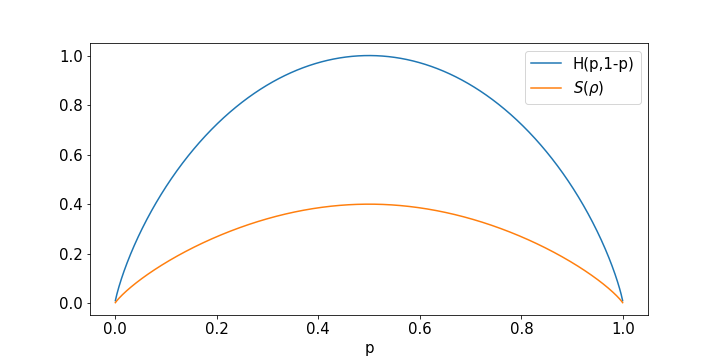
\includegraphics[width = 80mm]{./fig/ex11_12.png}
        \end{center}
    \end{figure}
\end{ex}

\begin{ex}
    \label{ex11.13}
    定理11.8(5)において,
    \begin{align*}
        \rho = \sum_i p_i \ket{i}\bra{i}, \rho_i = \sigma
    \end{align*}
    とすると,
    \begin{align*}
        S\left( \rho \otimes \sigma \right) = S(\rho) + S(\sigma).
    \end{align*}
    \par
    また,
    \begin{align*}
        \rho = \sum_i p_i \ket{i}\bra{i} \\
        \sigma = \sum_j q_j \ket{\tilde{j}}\bra{\tilde{j}}
    \end{align*}
    とすると,
    \begin{align*}
        \rho \otimes \sigma =
        \sum_{i,j} p_i q_j
        \left( \ket{i} \otimes \ket{\tilde{j}} \right)
        \left( \bra{i} \otimes \bra{\tilde{j}} \right)
    \end{align*}
    なので,
    \begin{align*}
        S\left( \rho \otimes \sigma \right) =
        -\sum_{ij} p_i q_j \log \left[ p_i q_j \right]
        =
        -\sum_{i} p_i \log p_i
        -\sum_{j} qol,_j \log q_j
        =
        S(\rho) + S(\sigma).
    \end{align*}
\end{ex}


\begin{ex}
    \label{ex11.14}
    \begin{align*}
        \ket{AB}\mathrm{が純粋状態}, S(B|A)<0
        \longleftrightarrow
        S(A) > 0
        \longleftrightarrow
        A \mathrm{が純粋状態でない}
    \end{align*}
\end{ex}

\begin{ex}
    \label{ex11.15}
    測定後の状態$\rho'$は,
    \begin{align*}
        \rho'
        = M_1 \rho M_1^\dagger + M_2 \rho M_2^\dagger
        = \tr [\rho] \ket{0}\bra{0} = \ket{0}\bra{0}
    \end{align*}
    より, $S(\rho') = 0$であるから, $S(\rho) \geq S(\rho')$.
\end{ex}

\begin{ex}
    \label{ex11.16}
    $\rho^{AB}$は混合状態として.
    \begin{align*}
        \rho^{AB} = \sum \lambda_i \ket{i^{AB}} \bra{i^AB}
    \end{align*}
    とかくと,
    \begin{align*}
        \rho^A = \sum \lambda_i \rho^A_i,
        \rho^B = \sum \lambda_i \rho^B_i
    \end{align*}
    となる. また, $AB$の純粋化$ABR$は, $R$の正規直交基底$\{ \ket{i^R} \}$として,
    \begin{align*}
        \ket{ABR}  & = \sum_i \sqrt{\lambda_i} \ket{i^{AB}} \ket{i^R} \\
        \rho^{ABR} & =  \sum_{ij} \sqrt{\lambda_i \lambda_j}
        \ket{i^{AB}} \bra{j^{AB}} \otimes \ket{i^{R}} \bra{j^{R}}     \\
    \end{align*}
    とかけるので,
    \begin{align*}
        \rho^{AR} & =  \sum_{ij} \sqrt{\lambda_i \lambda_j}
        \tr_B \left[\ket{i^{AB}} \bra{j^{AB}} \right] \otimes \ket{i^{R}} \bra{j^{R}} \\
        \rho^{R}  & =  \sum_{i} \lambda_i \ket{i^{R}} \bra{i^{R}}
    \end{align*}
    を得る.
    \par
    以上より,
    \begin{align*}
         & \ \ \ \ \ \ \  S(A,B) = S(B) - S(A)
        \\
         & \longleftrightarrow
        \rho^{AR} = \rho^A \otimes \rho^R
        \\
         & \longleftrightarrow
        \sum_{ij} \lambda_i \lambda_j \rho_i^A \otimes \ket{j^R}\bra{j^R}
        =
        \sum_{ij} \sqrt{\lambda_i \lambda_j}
        \tr_B \left[\ket{i^{AB}} \bra{j^{AB}} \right] \otimes \ket{i^{R}} \bra{j^{R}}
        \\
         & \longleftrightarrow
        \tr_B \left[\ket{i^{AB}} \bra{j^{AB}} \right] = \delta_{ij} \rho_i^A
        \mathrm{\ \ \ かつ\ \ \ }
        \sum_{ij} \lambda_i \lambda_j \rho_i^A \otimes \ket{j^R} \bra{j^R}
        = \sum_i \lambda_i \rho_i^A \otimes \ket{i^R} \bra{i^R}
        \\
         & \longleftrightarrow
        \tr_B \left[\ket{i^{AB}} \bra{j^{AB}} \right] = \delta_{ij} \tr_B \left[ \ket{i^{AB}} \bra{i^{AB}} \right]
        \mathrm{\ \ \ かつ\ \ \ }
        \sum_{ij} \lambda_i \lambda_j \rho_i^A \otimes \ket{j^R} \bra{j^R}
        = \sum_{ij} \lambda_i \lambda_j \rho_j^A \otimes \ket{j^R} \bra{j^R}
        \\
         & \longleftrightarrow
        \{ \rho_i^B \} \mathrm{が互いに直交する台を持つ}
        \mathrm{\ \ \ かつ\ \ \ }
        \exists \rho \ \forall i \in \{ i \ |\  \lambda_i > 0 \} \ \rho_i = \rho
    \end{align*}
    最後の行の2つ目の主張については, 演習\ref{ex11.18}で示す.
\end{ex}

\begin{ex}
    \label{ex11.17}
\end{ex}

\begin{ex}
    \label{ex11.18}
    示すべきは,
    \begin{align*}
        \sum_{ij} p_i p_j \rho_i \otimes \ket{j}\bra{j}
        =
        \sum_{j} p_j \rho_j \otimes \ket{j}\bra{j}
        \longleftrightarrow
        \exists \rho \ \forall i \in \{ i \ |\  p_i > 0 \} \ \rho_i = \rho
    \end{align*}
    \par
    $\longrightarrow)$
    \begin{align*}
        \sum_{ij} p_i p_j \rho_i \otimes \ket{j}\bra{j}
        =
        \sum_{j} p_j \rho_j \otimes \ket{j}\bra{j}
        =
        \sum_{ij} p_i p_j \rho_j \otimes \ket{j}\bra{j}
    \end{align*}
    であり, 両辺の系Bに対する部分とレースを取ると,
    \begin{align*}
        \sum_{ij} p_i p_j (\rho_i - \rho_j) = 0
    \end{align*}
    なので, $p_i > 0$なる任意の$i$の状態$\rho_i$は全て等しい.
    \par
    $\longleftarrow)$
    明らか.
\end{ex}


\begin{ex}
    \label{ex11.19}
    \begin{align*}
        S \left( \frac{I}{d}\right)
        =
        S \left( \sum_i p_i U_i \rho U_i^\dagger \right)
        \geq
        \sum_i p_i S \left( U_i \rho U_i^\dagger \right)
        =
        \sum_i p_i S\left( \rho \right)
        =
        S\left( \rho \right)
    \end{align*}
    で等号は,
    \begin{align*}
        \rho = \frac{I}{d}
    \end{align*}
    で成立. ここで, ユニタリ$U$に対して,
    \begin{align*}
        S \left( U \rho U^\dagger \right)
        =
        - \tr \left[ U \rho U^\dagger \log U \rho U^\dagger\right]
        =
        - \tr \left[ U \rho U^\dagger U (\log \rho) U^\dagger\right]
        =
        - \tr \left[ \rho \log \rho\right]
        =
        S \left( \rho\right)
    \end{align*}
    が成り立つことを用いた.
\end{ex}

\begin{ex}
    \label{ex11.20}
\end{ex}

\begin{ex}
    \label{ex11.21}
    $[ \rho , \sigma] = 0$とすると, これらは同時対角化可能で,
    \begin{align*}
        \rho = \sum_i p_i \ket{i} \bra{i},
        \sigma = \sum_i q_i \ket{i} \bra{i}
    \end{align*}
    とすると, von Neumannエントロピーの凹性より, $0 \le \lambda \le 1$に対して,
    \begin{align*}
        H( \{ \lambda p_i + (1 - \lambda) q_i\})
         & =
        - \sum_{i} \left( \lambda p_i + (1 - \lambda) q_i \right) \log \left( \lambda p_i + (1 - \lambda) q_i \right)
        \\
         & =S( \lambda \rho + (1 - \lambda) \sigma)
        \\
         & \geq
        \lambda S (\rho) + (1- \lambda) S(\sigma)
        \\
         & =
        \lambda H (\{ p_i \}) + (1- \lambda) H(\{ q_i\})
    \end{align*}
    と, Shannonエントロピーの凹性を示せた.
\end{ex}

\begin{ex}
    \label{ex11.22}
    $[ \rho , \sigma] = 0$とすると, これらは同時対角化可能で,
    \begin{align*}
        \rho = \sum_i p_i \ket{i} \bra{i},
        \sigma = \sum_i q_i \ket{i} \bra{i}
    \end{align*}
    とすると,
    \begin{align*}
        f(p)
        = S(p \rho + (1-p)\sigma)
        = - \sum_i
        \left[ \left( p_i - q_i \right) p + q_i \right]
        \log \left[  \left( p_i - q_i \right) p + q_i \right]
    \end{align*}
    なので,
    \begin{align*}
        f''(p) = - \sum_i \frac{ (p_i - q_i)^2 }{p_i p + (1-p)q_i} \leq 0.
    \end{align*}
\end{ex}

\begin{ex}
    \label{ex11.23}
    (11.96)式で$B_1 = B_2 = B$とすれば良い.
\end{ex}

\begin{ex}
    \label{ex11.24}
    $ABC$の純粋化$ABCR$として,
    \begin{align*}
        S(A,B) = S(C,R) , \ S(A,B,C) = S(R)
    \end{align*}
    なので, (11.108)式より,
    \begin{align*}
        S(R) + S(B) \le S(C,R) + S(B,C).
    \end{align*}
\end{ex}

\begin{ex}
    \label{ex11.25}
\end{ex}

\begin{ex}
    \label{ex11.26}
    強い劣加法性から,
    \begin{align*}
        S(A) + S(B) - S(A,B) +
        S(A) + S(C) - S(A,C)
        =
        S(A:B) + S(A:C)
        \le
        2S(A).
    \end{align*}
    \par
    たとえば, $\ket{AB}$として, EPR状態
    \begin{align*}
        \ket{AB} = \frac{\ket{00} + \ket{11}}{\sqrt{2}}
    \end{align*} 
    を取ると, 
    \begin{align*}
        S(A:B) = 2 > S(A) = 1.
    \end{align*}
\end{ex}
\chapter{量子情報理論}

\begin{ex}
    \label{ex12.1}
    $\braket{\psi|\phi} = 0$であれば,
    \begin{align*}
        U\ket{0} = \ket{\psi}, U\ket{1} = \ket{\phi}
    \end{align*}
    なるユニタリ$U$が存在して,
    \begin{align*}
        \Qcircuit @C=1em @R=1em {
        \lstick{}        & \gate{U^\dagger} & \ctrl{1} & \gate{U} & \qw \\
        \lstick{\ket{0}} & \qw              & \targ    & \gate{U} & \qw \\
        }
    \end{align*}
    という回路を用いれば, $\ket{\psi}\ket{\psi}, \ket{\phi}\ket{\phi}$という状態を作り出せる.
\end{ex}

\begin{ex}
    \label{ex12.2}
    \begin{align*}
        \tr \left[
            \sum_y
            \left(\sqrt{E_y} \otimes U_y \right)\left( \sigma \otimes \ket{0}\bra{0} \right)\left(\sqrt{E_y} \otimes U_y^\dagger\right)
            \right]
         & =
        \tr \left[
            \sum_y
            \left(\sqrt{E_y} \sigma \sqrt{E_y} \right) \otimes \ket{y}\bra{y}
            \right]
        \\
         & =
        \sum_y\tr \left[\sqrt{E_y} \sigma \sqrt{E_y} \otimes \ket{y}\bra{y}
            \right]
        \\
         & =
        \sum_y\tr \left[\sigma E_y\right] =
        \tr \sigma = \tr \left[
            \sigma \otimes \ket{0}\bra{0}
            \right].
    \end{align*}
\end{ex}

\begin{ex}
    \label{ex12.3}

\end{ex}

\begin{ex}
    \label{ex12.4}
\end{ex}

\begin{ex}
    \label{ex12.5}
    定理12.2(1)より, ある$\epsilon$を固定して,
    \begin{align*}
        \forall \delta > 0 \ \exists n_0 \in \mathbb{N} \ \forall n \ge n_0 \ \ P\left( X \in T(n, \epsilon) \right) \ge 1 - \delta
    \end{align*}
    である. 1情報記号のデータ圧縮に必要なビット数$A(n, \epsilon)$として,
    \begin{align*}
        A(n,\epsilon) & =
        H(X) P \left(X \in T(n,\epsilon) \right) + \frac{\log d^n}{n} P \left(X \notin T(n,\epsilon) \right)
        \\
                      & \le
        R  P \left(X \in T(n,\epsilon) \right) + \log d \left(1 - P \left(X \in T(n,\epsilon) \right)\right)
        \\
                      & \le
        R + \delta \log d
    \end{align*}
    なので,
    \begin{align*}
        \forall \delta > 0 \ \exists n_0 \in \mathbb{N} \ \forall n \ge n_0 \ \ |A(n,\epsilon)-R| \le \delta \log d.
    \end{align*}
\end{ex}

\begin{ex}
    \label{ex12.6}
    \begin{align*}
        C_X = p^{4 - \wt{X}} (1-p)^{\wt{X}}
    \end{align*}
\end{ex}

\begin{ex}
    \label{ex12.7}
    コラム12.4で, $V=I$とすれば良い.
\end{ex}

\begin{ex}
    \label{ex12.8}
    定理12.6の証明の式(12.51)で式(9.141)を用いて,
    \begin{align*}
        \bar{F} \ge F\left( \rho^{\otimes n}, D^n \circ C^n\right)
    \end{align*}
    すれば良い.
\end{ex}

\begin{ex}
    \label{ex12.9}
    (1)\
    $X$の確率分布関数を
    \begin{align*}
        p_X(0) = q, \ p_X(1) = 1 - q
    \end{align*}
    とすると$Y$の確率分布関数は
    \begin{align*}
        p_Y(0) = q(1-p), \ p_Y(1) = (1-q)(1-p),\  p_Y(e) = p
    \end{align*}
    となるので,
    \begin{align*}
        H(X:Y)
         & = H(Y) - H(Y|X)                                                                        \\
         & = H(Y) - \sum_x p_X(x) H(Y|X=x)                                                        \\
         & = H(Y) - H_{bin}(p)                                                                    \\
         & = -q(1-p)\log q(1-p) - (1-q)(1-p)\log(1-p)(1-q) - p \log p + p \log p + (1-p)\log(1-p) \\
         & =(1-p) H_{bin}(q) \le (1-p) H_{bin}(1/2) = 1 - p
    \end{align*}
    を得るので, 消去チャンネルの容量は$1-p$.
    \par
    (2)\
    \begin{align*}
        p = H_{bin}(p)
    \end{align*}
    を満たす非ゼロの$p$を$p_0$とする. $p\le p_0$であれば, $p \le H_{bin}(p)$なので, $1 - H_{bin}(p) \le 1 - p$.
    \begin{figure}[H]
        \begin{center}
            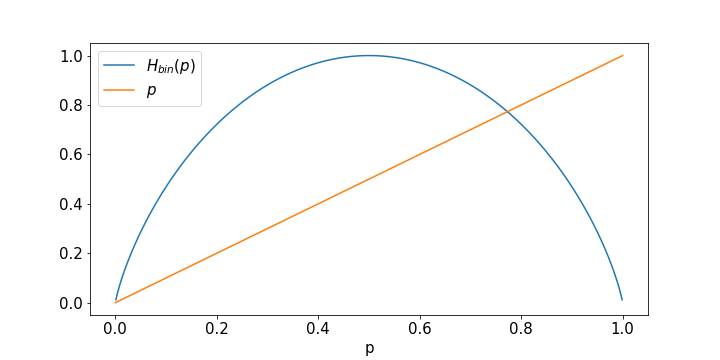
\includegraphics[width = 80mm]{./fig/ex12_9.png}
        \end{center}
    \end{figure}
\end{ex}

\begin{ex}
    \label{ex12.10}
    \begin{align*}
        X \xrightarrow{\mathscr{N}_1} Y \xrightarrow{\mathscr{N}_2} Z
    \end{align*}
    として,
    \begin{align*}
        C \left( \mathscr{N}_1 \circ \mathscr{N}_2 \right) = \max_{p_X(x)} H(X:Z) \\
        C \left( \mathscr{N}_1 \right) = \max_{p_X(x)} H(X:Y)                     \\
        C \left( \mathscr{N}_2 \right) = \max_{p_Y(y)} H(Y:Z)
    \end{align*}
    であることと, 定理11.5より,
    \begin{align*}
        C \left( \mathscr{N}_1 \circ \mathscr{N}_2 \right)
        \le \min \left(C \left( \mathscr{N}_1 \right), C \left( \mathscr{N}_2 \right)\right)
    \end{align*}
    を得る.
\end{ex}

\begin{ex}
    \label{ex12.11}
    \begin{align*}
        \chi \left( \qo \right) = \max_\rho \max_{\left\{ p_j,
            \rho_j \right\} \mathrm{ \ subject \ to} \ \rho = \sum_j p_j \rho_j }
        \left[ S\left( \qo(\rho)\right) - \sum_j p_j S\left( \qo(\rho_j) \right) \right]
    \end{align*}
    とかけることに注目する.
    \par
    まず, $\rho$を固定する.
    \begin{align*}
        \rho_j = \sum_k q_j^k \ket{\psi_j^k}\bra{\psi_j^k}
    \end{align*}
    とすると, エントロピーの凹性と$\qo$の線型性より,
    \begin{align*}
        S \left( \qo(\rho_j)\right) \ge
        \sum_k q_j^k S \left( \qo(\ket{\psi_j^k}\bra{\psi_j^k}) \right)
    \end{align*}
    を得る. 式(11.79)より, この等号成立条件が$\rho_j$が純粋状態の時であることから,
    \begin{align*}
        \max_{\left\{ p_j,
            \rho_j \right\} \mathrm{ \ subject \ to} \ \rho = \sum_j p_j \rho_j }
        \left[ S\left( \qo(\rho)\right) - \sum_j p_j S\left( \qo(\rho_j) \right) \right]
    \end{align*}
    を実現するアンサンブル$\{p_j, \rho_j \}$は純粋状態だけからなることがわかる.
    \par
    次に, $\rho = \sum_j p_j \rho_j$を動かす. 任意の$\rho$は, 独立な純粋状態$\rho_1,\ \rho_2 , ..., \rho_{d^2}$の線形和でかけることから, $\max$を取るべきアンサンブルとしては, 高々$d^2$個の純粋状態だけからなるアンサンブルを考えれば十分.
\end{ex}

\begin{ex}
    \label{ex12.12}
\end{ex}

\begin{ex}
    \label{ex12.13}
    $\qo$が$\qo_1, \qo_2$を用いて,
    \begin{align*}
        \qo = p \qo_1 + ( 1 - p) \qo_2
    \end{align*}
    とかけるとする. 入力$\rho$に対する$\qo, \qo_1, \qo_2$のw行列を$W, W_1, W_2$とすると,
    \begin{align*}
        W = p W_1 + (1-p) W_2
    \end{align*}
    を得る.よって, エントロピーの凹性より,
    \begin{align*}
        S \left( \rho, p \qo_1 + (1-p)\qo_2 \right)
        =
        S(pW_1 + (1-p)W_2 )
        \ge
        p S(W_1) + (1-p) S(W_2)
        =
        p S \left( \rho, \qo_1\right) + (1-p) S \left( \rho, \qo_2\right).
    \end{align*}
\end{ex}

\begin{ex}
    \label{ex12.14}
\end{ex}

\begin{ex}
    \label{ex12.15}
    1つの例として, 強い劣加法性
    \begin{align*}
        S\left( \rho^{R'' E_1'' E_2''}\right) + S\left( \rho^{E_1''}\right)
        \le S\left( \rho^{R'' E_1''}\right) + S\left( \rho^{E_1'' E_2''}\right)
    \end{align*}
    から関係式を導いてみる.
    上の強い劣加法性から, 定理12.10の第2不等号が導かれたことを思い出すと,
    \begin{align*}
        S\left(\rho''\right) - S\left(\rho'\right)
        \le
        S\left( \rho, \qo_2 \circ \qo_1\right)
        -
        S\left( \rho, \qo_1\right)
        =
        S\left( \rho^{E_1'' E_2''} \right) - S\left( \rho^{E_1''}\right).
    \end{align*}
    ここで, $\rho^{E_1'' E_2''}$,$\rho^{E_1''}$を$\qo_1, \qo_2$の演算要素$\{ E_i \}, \{ F_i\}$で書くことを考える. 量子演算を作用させる前の$QE_1'' E_2''$の状態$\rho^Q \otimes \ket{0}\bra{0} \otimes \ket{0}\bra{0}$とすると,
    \begin{align*}
        \rho^{Q E_1'' E_2''}
        =
        \sum_{i,j,k,l}  F_i E_j \rho^Q E_k^\dagger F_l^\dagger \otimes \ket{j} \bra{k} \otimes \ket{i}\bra{l}
    \end{align*}
    なので,
    \begin{align*}
        \rho^{E_1'' E_2''}
         & = \tr_Q \rho^{Q E_1'' E_2''}
        = \sum_{i,j,k,l}  \tr_Q \left[ F_i E_j \rho^Q E_k^\dagger F_l^\dagger \right] \ket{j} \bra{k} \otimes \ket{i}\bra{l}
        \\
        \rho^{E_1'' }
         & = \tr_{Q E_2} \rho^{Q E_1'' E_2''}
        =\sum_{i,j,k}  \tr_Q \left[ F_i E_j \rho^Q E_k^\dagger F_i^\dagger \right] \ket{j} \bra{k}
    \end{align*}
    \par
    他の組み合わせについては, arXiv:quant-ph/0011036に示してある.
    \par
\end{ex}

\begin{ex}
    \label{ex12.16}
    定理12.10の第1等号の成立条件で示した.
\end{ex}

\begin{ex}
    \label{ex12.17}
    示すべきは,
    \begin{align*}
        \forall t \in \mathbb{R} \ \
        \sum_{j=1}^d \max\left( x_j - t, 0\right)
        \le
        \sum_{j=1}^d \max\left( y_j - t, 0\right)
        \longleftrightarrow
        \forall k \in \{1, 2, ..., d \} \ \
        \sum_{j=1}^k x_j^\downarrow
        \le
        \sum_{j=1}^k y_j^\downarrow
    \end{align*}
    \par
    $\longrightarrow)$
    $k = 1,2, ..., d$ に対して$t = y_k^\downarrow$とすれば,
    \begin{align*}
        \sum_{j=1}^k \left( y_j^\downarrow -  y_k^\downarrow\right)
        =
        \sum_{j=1}^d \max\left( y_j^\downarrow  -  y_k^\downarrow, 0\right)
        \ge
        \sum_{j=1}^d \max\left( x_j^\downarrow -  y_k^\downarrow, 0\right)
        \ge
        \sum_{j=1}^k \max\left( x_j^\downarrow -  y_k^\downarrow, 0\right)
        \ge
        \sum_{j=1}^k \left(x_j^\downarrow  - y_k^\downarrow \right)
    \end{align*}
    より
    \begin{align*}
        \sum_{j=1}^k y_j^\downarrow
        \ge
        \sum_{j=1}^k x_j^\downarrow
    \end{align*}
    を得る.
    \par
    $\longleftarrow)$
    任意の実数$t$をとってくると,
    \begin{enumerate}
        \item $\exists i \in \{ 1,2, ..., d-1\} \ \  x_i^\downarrow \ge t \ge x_{i+1}^\downarrow$
        \item $t \ge x^\downarrow_1$
        \item $x^\downarrow_d \ge t$
    \end{enumerate}
    のいずれかを満たし, いずれの場合でも
    \begin{enumerate}
        \item $ \sum_{j=1}^d \max(x_j - t, 0)
                  =
                  \sum_{j=1}^i (x_j^\downarrow - t)
                  \le
                  \sum_{j=1}^i (y_j^\downarrow - t)
                  \le
                  \sum_{j=1}^i \max(y_j^\downarrow - t,0)
                  \le
                  \sum_{j=1}^d \max(y_j - t,0)$
        \item $\sum_{j=1}^d \max(x_j - t, 0) = 0 \le \sum_{j=1}^d \max(y_j - t,0)$
        \item $ \sum_{j=1}^d \max(x_j - t, 0)
                  =
                  \sum_{j=1}^d (x_j^\downarrow - t)
                  \le
                  \sum_{j=1}^d (y_j^\downarrow - t)
                  \le
                  \sum_{j=1}^d \max(y_j - t,0)$
    \end{enumerate}
    のように,
    \begin{align*}
        \sum_{j=1}^d \max\left( x_j - t, 0\right)
        \le
        \sum_{j=1}^d \max\left( y_j - t, 0\right)
    \end{align*}
    が示せた.
\end{ex}

\begin{ex}
    \label{ex12.18}
    $x^1 , x^2 \prec y$, $ 0 \le \lambda \le 1$とすると,
    $k = 1, 2, ..., d$に対して,
    \begin{align*}
        \sum_{j=1}^k \lambda x_j^{1 \downarrow} + (1-\lambda) x_j^{2 \downarrow}
        \le
        \sum_{j=1}^k y_j^\downarrow
    \end{align*}
    であり,
    \begin{align*}
        \sum_{j=1}^d \lambda x_j^{1 \downarrow} + (1-\lambda) x_j^{2 \downarrow}\le
        \sum_{j=1}^d y_j^\downarrow
    \end{align*}
    であるので, $\lambda x_j^{1} + (1-\lambda) x_j^{2} \prec y$なので, $\{x | x \prec y\}$は凸集合.
\end{ex}

\begin{ex}
    \label{ex12.19}
    示すべきは, $x \prec y$ならば$x' \prec y'$, つまり$l = 1,2, ..., d-1$に対して,
    \begin{align*}
        \sum_{i=1}^l x_i'^\downarrow
        \le
        \sum_{i=1}^l y_i'^\downarrow
    \end{align*}
    が成立し, $l = d-1$で等号が成立すること.
    \par
    次のような$k$を定める;
    \begin{align*}
        y_1^\downarrow \le y_2^\downarrow \le ... \le y_k^\downarrow \le (1-t) y_1^\downarrow + t y_j^\downarrow \le y_{k+1}^\downarrow \le y_{k+2}^\downarrow \le ... \le y_{j}^\downarrow
        \le ... \le y_d^\downarrow
    \end{align*}
    また, $l = 1,2, ..., d-1$として,
    \begin{align*}
        \sum_{i=1}^l x_i'^\downarrow
        =
        \sum_{i=1}^{l+1} x_i^\downarrow - x_1^\downarrow
        \le
        \sum_{i=1}^{l+1} y_i^\downarrow - t y_1^\downarrow - (1-t)y_j^\downarrow
    \end{align*}
    が成立.
    \par
    \underline{$l \le k -1 $のとき}\
    \begin{align*}
        \sum_{i=1}^l y_i'^\downarrow = \sum_{i=2}^{l+1} y_i^\downarrow
    \end{align*}
    なので,
    \begin{align*}
        \sum_{i=1}^l x_i'^\downarrow
        \le
        \sum_{i=1}^{l+1} y_i^\downarrow - t y_1^\downarrow - (1-t)y_j^\downarrow
        =
        \sum_{i=1}^l y_i'^\downarrow + (1-t)y_1^\downarrow - (1-t)y_j^\downarrow
        \le
        \sum_{i=1}^l y_i'^\downarrow +  y_{k+1}^\downarrow - y_j^\downarrow
        \le
        \sum_{i=1}^l y_i'^\downarrow.
    \end{align*}
    \par
    \underline{$k \le l \le j - 1 $のとき}\
    \begin{align*}
        \sum_{i=1}^l y_i'^\downarrow = \sum_{i=2}^{l} y_i^\downarrow + (1-t) y_1^\downarrow + t y_j^\downarrow
    \end{align*}
    なので,
    \begin{align*}
        \sum_{i=1}^l x_i'^\downarrow
        \le
        \sum_{i=1}^{l+1} y_i^\downarrow - t y_1^\downarrow - (1-t)y_j^\downarrow
        =
        \sum_{i=1}^l y_i'^\downarrow - y_j^\downarrow + y_{l+1}^\downarrow
        \le
        \sum_{i=1}^l y_i'^\downarrow
    \end{align*}
    \par
    \underline{$j \le l $のとき}\
    \begin{align*}
        \sum_{i=1}^l y_i'^\downarrow = \sum_{i=2}^{j-1} y_i^\downarrow + \sum_{i=j+1}^{l+1} y_i^\downarrow + (1-t) y_1^\downarrow + t y_j^\downarrow
        =
        \sum_{i=2}^{l+1} y_i^\downarrow + (1-t) y_1^\downarrow - (1- t)  y_j^\downarrow
    \end{align*}
    なので,
    \begin{align*}
        \sum_{i=1}^l x_i'^\downarrow
        \le
        \sum_{i=1}^{l+1} y_i^\downarrow - t y_1^\downarrow - (1-t)y_j^\downarrow
        =
        \sum_{i=1}^l y_i'^\downarrow
    \end{align*}
    \par
    \underline{$l = d - 1 $のとき}\
    \begin{align*}
        \sum_{i=1}^{d-1} x_i'^\downarrow
        =
        \sum_{i=1}^{d} y_i^\downarrow - t y_1^\downarrow - (1-t)y_j^\downarrow
        =
        \sum_{i=1}^l y_i'^\downarrow
    \end{align*}
\end{ex}

\begin{ex}
    \label{ex12.20}
    $\rho_\psi$の台をAliceの状態空間とすれば良い.
\end{ex}

\begin{ex}
    \label{ex12.21}
    \begin{align*}
        \tr_B \ket{\psi}\bra{\psi}
         & = 0.4 \ket{0}\bra{0} + 0.4 \ket{1}\bra{1} + 0.1 \ket{2}\bra{2} + 0.1 \ket{3}\bra{3}
        \\
        \tr_B \ket{\phi}\bra{\phi}
         & = 0.5 \ket{0}\bra{0} + 0.25 \ket{1}\bra{1} + 0.25 \ket{2}\bra{2}
    \end{align*}
    より, $\tr_B \ket{\psi}\bra{\psi} \nprec \tr_B \ket{\phi}\bra{\phi}$
    なので, 定理12.25より$\ket{\psi}$から$\ket{\phi}$への変換はLOCCではできない.
\end{ex}

\begin{ex}
    \label{ex12.22}

\end{ex}

\begin{ex}
    \label{ex12.23}
    教科書の議論より, LOCCにより, $\ket{\psi} = \sum_x \sqrt{x} \ket{x_A}\ket{x_B}$から$S(\rho_\psi)$個のBell状態が作れることがわかっている. ここで, $\rho_\psi = \tr_A \ket{\psi}\bra{\psi}$.
    LOCCによって$S (< S(\rho_\psi))$のBell状態から$\ket{\psi}$が作れるとすると, $S(\rho_\psi)$個のBell状態が作れる. つまり, LOCCによって, $S (< S(\rho_\psi))$のBell状態から $S(\rho_\psi)$個のBell状態が作れる事になるが, これは演習\ref{ex12.24}より矛盾. したがって, 教科書にあるもつれの希釈手続きが最適である.
\end{ex}

\begin{ex}
    \label{ex12.24}
    純粋状態$\ket{\psi}, \ket{\phi}$は,
    \begin{align*}
        \ket{\psi} = \sum_{i=1}^{\mathrm{Sch}(\lambda_\psi)} \sqrt{\lambda_{\psi i}}\ket{i}_A \ket{i}_B , \
        \ket{\phi} = \sum_{i=1}^{\mathrm{Sch}(\lambda_\phi)} \sqrt{\lambda_{\phi i}}\ket{\tilde{i}}_A \ket{\tilde{i}}_B
    \end{align*}
    とかける. ここで,
    \begin{align*}
        \sum_{i=1}^{\mathrm{Sch}(\lambda_\psi)} \lambda_{\psi i}^\downarrow
        = \sum_{i=1}^{\mathrm{Sch}(\lambda_\phi)} \lambda_{\phi i}^\downarrow= 1                     \\
        \forall i \in \{ 1,2, ..., \mathrm{Sch}(\lambda_\psi) \} \ \ \lambda_{\psi i}^\downarrow > 0 \\
        \forall i \in \{ 1,2, ..., \mathrm{Sch}(\lambda_\phi) \} \ \ \lambda_{\phi i}^\downarrow > 0
    \end{align*}
    である.
    定理12.25より, LOCCにより$\ket{\psi} \to \ket{\phi}$という変換が可能であるとすると, $\lambda_\psi \prec \lambda_\phi$. もし, $\mathrm{Sch}(\lambda_\psi) < \mathrm{Sch}({\lambda_\phi})$とすると,
    \begin{align*}
        0 =
        \sum_{i=1}^{\mathrm{Sch}(\lambda_{\psi})} \lambda_{\psi i}^\downarrow
        -
        \sum_{i=1}^{\mathrm{Sch}(\lambda_{\phi})} \lambda_{\phi i}^\downarrow
        =
        \sum_{i=1}^{\mathrm{Sch}(\lambda_{\psi})} ( \lambda_{\psi i}^\downarrow - \lambda_{\phi i}^\downarrow)
        +
        \sum_{i=\mathrm{Sch}(\lambda_{\psi})+1}^{\mathrm{Sch}(\lambda_{\phi})} \lambda_{\phi i}
        > 0
    \end{align*}
    と矛盾. したがって, LOCCによる$\ket{\psi} \to \ket{\phi}$という変換によって, Schmidt数は増加しない.
    \par
    $d$次元状態空間上の純粋状態$\ket{\psi}, \ket{\phi}$が,
    \begin{align*}
        \ket{\psi} & = \left( \frac{\ket{00} + \ket{11}}{\sqrt{2}}\right)^{\otimes k} \ket{\mathrm{ABがもつれてない2qubit状態}}^{\otimes{d-k}}  \\
        \ket{\phi} & =  \left( \frac{\ket{00} + \ket{11}}{\sqrt{2}}\right)^{\otimes l} \ket{\mathrm{ABがもつれてない2qubit状態}}^{\otimes{d-l}}
    \end{align*}
    とする. $\ket{\psi}, \ket{\phi}$はそれぞれAliceとBobが$k, l$個のBell状態を共有している. ここで, $k < l$とすると, $\mathrm{Sch}(\lambda_\psi) = 2^k < \mathrm{Sch}(\lambda_\phi) = 2^l$なので, $\ket{\psi} \to\ket{\phi}$という変換はLOCCによってできない. つまり, AliceとBobの共有するBell状態の数は,LOCCで増加しない.
\end{ex}

\begin{ex}
    \label{ex12.25}
    秘密鍵$n!/2$, 公開鍵$2n$.
\end{ex}

\begin{ex}
    \label{ex12.26}
    $(b_k,b_k') = (0,0)$のとき, Bobは$\ket{\psi_{{a_k}0}} = \ket{a_k}$を$Z$の固有状態を基底とした測定を行い, 測定値$a_k'$は確率1で$a_k$と等しくなる. $(b_k,b_k') = (1,0)$のとき, Bobは$\ket{\psi_{{a_k}1}} = \ket{a_k}$を$Z$の固有状態を基底とした測定を行い, 測定値$a_k'$は確率1/2で$a_k$, 確率1/2で$\bar{a}_k$というようにランダムに得られる. $(b_k,b_k') = (0,1),(b_k,b_k') = (1,1)$のときも同様.
\end{ex}

\begin{ex}
    \label{ex12.27}
    (1) \
    \begin{align*}
        \epsilon = \mu - 2 \delta \ge 0
    \end{align*}
    とする. 2nビットのうち$\mu n$ビットが誤ってるとする. $2n$ビットから$n$ビットの検査ビットを選んだ時に, 検査ビット中の誤りが$\delta n$より小さくなる確率$p$は,
    \begin{align*}
        p = \sum_{i=0}^{\delta n - 1} \frac{{}_{\mu n} C _{i} \times {}_{2n - \mu n} C _{n - i}}{{}_{2n} C_n}.
    \end{align*}
    ここで,
    \begin{align*}
        a_i \equiv {}_{\mu n} C _{i} \times {}_{2n - \mu n} C _{n - i}
    \end{align*}
    とすると, $i = 0, 1, ..., \delta n - 2$に対して,
    \begin{align*}
        \frac{a_{i+1}}{a_i} = \frac{
            \frac{n+1}{i+1} - 1
        }{
            \frac{n+1}{\mu n - i } - 1
        }
        > 1
    \end{align*}
    より, $a_i$は単調増加なので,
    \begin{align*}
        p =
        \sum_{i=0}^{\delta n - 1} \frac{a_i}{{}_{2n} C_n} <
        \delta n \frac{a_{\delta n}}{{}_{2n} C_n} <
        \delta n
        \frac{{}_{\mu n} C _{\delta n} \times {}_{2n - \mu n} C _{n - \delta n}}{{}_{2n} C_n}
    \end{align*}
    を得る.
    \par
    (2)\
    \begin{align*}
        \frac{b}{a} = t, an = s
    \end{align*}
    とすると,
    \begin{align*}
        2^{an H \left( \frac{b}{a}\right)} & = \left[ t^{t} (1-t)^{1-t}\right]^{-s} \\
        {}_{an} C_{bn}                     & = {}_s C_{st}
    \end{align*}
    とかける.
    スターリングの公式より,
    \begin{align*}
        \frac{\sqrt{2 \pi}}{e^2} \frac{s^{s + \frac{1}{2}}}{(st)^{st + \frac{1}{2}} (s(1-t))^{s(1-t) + \frac{1}{2}}}
        \le
        \frac{s!}{(st)! (s - st)!}={}_s C_{st}
        \le
        \frac{e}{2 \pi} \frac{s^{s + \frac{1}{2}}}{(st)^{st + \frac{1}{2}} (s(1-t))^{s(1-t)+ \frac{1}{2}}}.
    \end{align*}
    よって,
    \begin{align*}
        \frac{2^{an H \left( \frac{b}{a}\right)}}{{}_{an} C_{bn}}
         & =
        \frac{\left[ t^{t} (1-t)^{(1-t)}\right]^{-s}}{{}_s C_{st}}
        \\
         & \ge
        \frac{2 \pi}{e}
        \frac{(st)^{st + \frac{1}{2}} (s(1-t))^{s(1-t)+ \frac{1}{2}}}{s^{s + \frac{1}{2}} \left[ t^{t} (1-t)^{1-t}\right]^s}
        \\
         & =
        \frac{2 \pi}{e}
        \left(
        \frac{st \cdot s(1-t)}{s}
        \right)^{\frac{1}{2}}
        \left(
        \frac{(st)^t (s(1-t))^{1-t}}{s t^t (1-t)^{1-t}}
        \right)^{s}
        =
        \frac{2 \pi}{e}
        \sqrt{st(1-t)}
    \end{align*}
    よって, 任意の$t$に対して,
    \begin{align*}
        s > \frac{e^2}{4 \pi^2 t(1-t)}
    \end{align*}
    を満たす程十分大きな$s$を取れば,
    \begin{align*}
        \frac{2^{an H \left( \frac{b}{a}\right)}}{{}_{an} C_{bn}} \ge 1.
    \end{align*}
    もう一方の不等号についても同様に示せる.
    \par
    (3)\
    問題文で与えられた不等式と(2)で示した不等式より,
    \begin{align*}
        p
         & <
        \delta n
        \frac{{}_{\mu n} C _{\delta n} \times {}_{2n - \mu n} C _{n - \delta n}}{{}_{2n} C_n}
        \\
         & <
        \delta n (2n+1) \frac{
            2^{\mu n \left( 1 - 2 \left(  \frac{\mu}{\delta} - \frac{1}{2}\right)^2\right)}
            2^{(2 - \mu )n \left( 1 - 2 \left(  \frac{2 - \mu}{ 1 - \delta} - \frac{1}{2}\right)^2\right)}
        }
        {
            2^{\frac{n}{2}}
        }
        \\
         & =
        \delta n (2n+1) 2^{\frac{3n}{2}}
        2^{-2 n \left( \mu \left(\frac{\mu}{\delta} - \frac{1}{2}\right)^2
                + (2 - \mu) \left(\frac{2 - \mu}{ 1 - \delta} - \frac{1}{2}\right)^2 \right)}
        \\
         & =
        \delta n (2n+1) 2^{\frac{3n}{2}}
        2^{
                -\frac{n}{2}
                \left[
                    \mu \frac{\epsilon^2}{\delta^2}
                    +  (2 - \mu)\frac{(2\epsilon + 3 (1 - \delta))^2}{ (1 - \delta)^2}
                    \right]
            }
        \\
         & <
        \delta n (2n+1) 2^{\frac{3n}{2}}
        2^{
                -\frac{n}{2}
                \left[
                    \mu \frac{\epsilon^2}{\delta^2}
                    +  (2 - \mu)\frac{4 \epsilon^2}{ (1 - \delta)^2}
                    \right]
            }
        \\
         & <
        \delta n (2n+1) 2^{\frac{3n}{2}}
        2^{
                -\frac{n}{2}
                \left[
                    \mu {\epsilon^2}
                    +  (2 - \mu){4 \epsilon^2}
                    \right]
            }
        \\
         & <
        \delta n (2n+1)
        2^{
                -\frac{n}{2}
                \left[
                    3 + (8 - 3 \mu) \epsilon^2
                    \right]
            }
        = 2^{- O (\epsilon^2 n)}.
    \end{align*}
\end{ex}

\begin{ex}
    \label{ex12.28}
    $(a', b) = (0, 1)$のとき, Bobが状態$\ket{\psi}$を$Z$基底で測定して, 固有値$+1$の方を得る. このとき$\ket{\psi} = \ket{0}$つまり$a = a' = 0$. \ $(a', b) = (1, 1)$のときも同様に示せる
\end{ex}

\begin{ex}
    \label{ex12.29}
\end{ex}

\begin{ex}
    \label{ex12.30}
    $\ln(1-x)$のTaylor展開
    \begin{align*}
        \ln(1-x) = -x + O(x^2)
    \end{align*}
    を用いて, 
    \begin{align*}
        S(\rho_\mathrm{max})
        &=
        -(1-2^{-s}) \log(1 - 2^{-s}) - 2^{-s} \log \frac{2^{-s-2n}}{1 - 2^{-2n}}
        \\
        &=
        \frac{1 - 2^{-s}}{\ln 2} \left( 2^{-s} + O(2^{-2s})\right)
        +
        2^{-s}\left( s + 2n\right) + 2^{-s}\left( - 2^{-n} + O(2^{-2n})\right)
        \\
        &=
         \left(2n + s + \frac{1}{\ln2} \right)2^{-s} + O(2^{-2s}).
    \end{align*}
    最後の等号では$s<n$を用いた.
\end{ex}

\begin{ex}
    \label{ex12.31}
    Eveがチャンネル全ての制御ができるとすると, AliceがBobに送信した情報を, 
    \begin{align*}
        F\left( \rho, \ket{\beta_{00}}^{\otimes n} \right) > 1 - 2^{-s}
    \end{align*}
    を満たすように
    \begin{align*}
        \rho = \sum_x p_x \rho_x
    \end{align*}
    と書き換えることができてしまう. $\rho$をAliceとBobがPOVM$\{ E_y\}$によって測定して得た結果$Y$とEveが持っている$\rho$に関する情報$X$の相互情報量は, Holevo限界, エントロピーの非負性, 演習\ref{ex12.30}より, 
    \begin{align*}
        H(X:Y) \le S(\rho) - \sum_x p_x S \left(\rho_x \right) \le S(\rho) 
        < \left(2n + s + \frac{1}{\ln2} \right)2^{-s} + O(2^{-2s}).
    \end{align*}
\end{ex}

\begin{ex}
    \label{ex12.32}
    例えば, ビット反転については, 
    \begin{align*}
        \Pi_{bf} = \frac{I \otimes I - Z \otimes Z}{2}, I - \Pi_{bf} = \frac{I \otimes I + Z \otimes Z}{2}
    \end{align*}
    とかけるので.
\end{ex}

\begin{ex}
    \label{ex12.33}
\end{ex}

\begin{ex}
    \label{ex12.34}
\end{ex}

\begin{ex}
    \label{ex12.35}
\end{ex}

\begin{ex}
    \label{ex12.36}
    明らか.
\end{ex}
\renewcommand\thechapter{\Alph{chapter}}
\setcounter{chapter}{3}
\chapter{整数論}

\begin{ex}
\end{ex}


\begin{ex}
\end{ex}


\begin{ex}
\end{ex}

\begin{ex}
\end{ex}

\begin{ex}
\end{ex}

\begin{ex}
\end{ex}


\begin{ex}
\end{ex}

\begin{ex}
\end{ex}

\begin{ex}
\end{ex}

\begin{ex}
\end{ex}

\begin{ex}
\end{ex}


\begin{ex}
\end{ex}

\begin{ex}
\end{ex}

\begin{ex}
\end{ex}

\begin{ex}
\end{ex}

\begin{ex}
\end{ex}

\begin{ex}
\end{ex}

\begin{ex}
\end{ex}




\begin{ex}
    \begin{align*}
        q_1 p_0 - p_1 q_0 & = -1
        \\
        q_n p_{n-1} - p_n q_{n-1}
                          & =
        (a_n q_{n-1} + q_{n-2}) p_{n-1} - (a_n p_{n-1} + p_{n-2}) q_{n-1}
        =
        (-1)(q_{n-1} p_{n-2} - p_{n-1} q_{n-2})
    \end{align*}
    なので, 帰納法より,
    \begin{align*}
        q_n p_{n-1} - p_n q_{n-1}  = (-1)^n.
    \end{align*}
    \par
    $p_n, q_n$の最大公約数$g_n$として, $p_n = g_n p_n'$などと書くと,
    \begin{align*}
        g_n g_{n-1} \left(q_n' p_{n-1}' - p_n' q_{n-1}' \right) = (-1)^n.
    \end{align*}
    ここで,
    \begin{align*}
         & \frac{q_n' p_{n-1}' - p_n' q_{n-1}'}{p_n' p_{n-1}'}
        =
        \frac{q_n'}{p_n'} - \frac{q_{n-1}'}{p_{n-1}'}
        =
        \frac{q_n}{p_n} - \frac{q_{n-1}}{p_{n-1}}
        \begin{cases}
            > 0 & (n : \mathrm{even}) \\
            < 0 & (n: \mathrm{odd})
        \end{cases}
        \\ &\to
        q_n' p_{n-1}' - p_n' q_{n-1}'
        \begin{cases}
            > 0 & (n : \mathrm{even}) \\
            < 0 & (n: \mathrm{odd})
        \end{cases}
    \end{align*}
    であるから,
    \begin{align*}
        g_n g_{n-1} = 1
    \end{align*}
    となり, $g_n, g_{n-1}$は正の整数なので,
    \begin{align*}
        g_n = g_{n-1} = 1
    \end{align*}
    を得る.
\end{ex}
\renewcommand\thechapter{\Alph{chapter}}
\setcounter{chapter}{5}
\chapter{Liebの定理の証明}

\begin{ex}
    \label{exf.1}
    $A \le B$とすると, 任意の状態$\ket{\psi}$に対して,
    \begin{align*}
        \braket{ \psi | X^\dagger (B - A) X | \psi} \ge 0
    \end{align*}
    なので,
    \begin{align*}
        X^\dagger B X \ge X^\dagger A X.
    \end{align*}
\end{ex}

\begin{ex}
    \label{exf.2}
    明らか.
\end{ex}

\begin{ex}
    \label{exf.3}
    明らか.
\end{ex}

\begin{ex}
    \label{exf.4}
    (1) \par
    (2)\
    $A$はHermiteなので,
    \begin{align*}
        A = \sum_i \lambda_i \ket{i} \bra{i}
    \end{align*}
    として,
    \begin{align*}
        || A ||
         & = \max | \braket{u | A | u} | \ \mathrm{subject \ to } \braket{u|u} = 1                      \\
         & = \max \left|\sum_i \lambda_i |c_i|^2 \right| \ \mathrm{subject \ to \ } {\sum_i}|c_i|^2 = 1 \\
         & = | \lambda |
    \end{align*}
\end{ex}

\begin{ex}
    \label{exf.5}
    $AB, BA$の固有多項式$f_{AB}(x), f_{BA}(x)$とかく.
    \par
    $A$が正則ならば,
    \begin{align*}
        f_{AB}(x) =
        \det\left( xI - AB\right)
        = \det\left( A^{-1} x I A - A^{-1} ABA\right)
        = \det\left( xI - BA \right)
        = f_{BA}(x).
    \end{align*}
    \par
    $A$が非正則とする.
    上に示した通り, $A(y) = A + yI$として, $\det A(y) \neq 0$なる$y$に対して,
    \begin{align*}
        f_{A(y)B}(x) = f_{BA(y)}(x)
    \end{align*}
    である. ここで,
    $\det A(y)$は$y$に関する$n$次なので, $\det A(y) = 0$なる$y$は高々$n$個であることと固有多項式の連続性より,
    上式で $\det A(y) = 0$なる$y$を避けるように, $y \to 0$として,
    \begin{align*}
        f_{AB}(x) = f_{BA}(x).
    \end{align*}
\end{ex}

\begin{ex}
    \label{exf.6}
    演習\ref{exf.4},\ \ref{exf.5}より, $AB$がHermiteならば, $AB$の絶対値最大の固有値$\lambda$として,
    \begin{align*}
        \lambda = || AB || \le || BA ||.
    \end{align*}
\end{ex}

\begin{ex}
    \label{exf.7}
    $A$が正オペレータのとき, 
    \begin{align*}
        A \le I
         & \longleftrightarrow
        \forall \ket{\psi} \ \braket{\psi| I - A | \psi} | \ge 0 \\
         & \longleftrightarrow
         \forall \ket{\psi} \ 0 \le \braket{\psi| A | \psi}  \le \braket{\psi|\psi} \\
         & \longleftrightarrow
         \forall \ket{u}:\mathrm{単位ベクトル}  \ 0 \le \braket{u| A | u}  \le 1 \\
         & \longleftrightarrow
         || A || \le 1. \\
    \end{align*}
\end{ex}

\begin{ex}
    \label{exf.8}
    $A,B$が正オペレータのとき, $\tr AB \ge 0$なので, 
    \begin{align*}
        \tr X^\dagger A X = \tr A X X^\dagger \ge 0.
    \end{align*}
\end{ex}
\bibliographystyle{abbrv}
\bibliography{main.bib}
\end{document}